\documentclass[twoside]{book}

% Packages required by doxygen
\usepackage{fixltx2e}
\usepackage{calc}
\usepackage{doxygen}
\usepackage[export]{adjustbox} % also loads graphicx
\usepackage{graphicx}
\usepackage[utf8]{inputenc}
\usepackage{makeidx}
\usepackage{multicol}
\usepackage{multirow}
\PassOptionsToPackage{warn}{textcomp}
\usepackage{textcomp}
\usepackage[nointegrals]{wasysym}
\usepackage[table]{xcolor}

% Font selection
\usepackage[T1]{fontenc}
\usepackage[scaled=.90]{helvet}
\usepackage{courier}
\usepackage{amssymb}
\usepackage{sectsty}
\renewcommand{\familydefault}{\sfdefault}
\allsectionsfont{%
  \fontseries{bc}\selectfont%
  \color{darkgray}%
}
\renewcommand{\DoxyLabelFont}{%
  \fontseries{bc}\selectfont%
  \color{darkgray}%
}
\newcommand{\+}{\discretionary{\mbox{\scriptsize$\hookleftarrow$}}{}{}}

% Page & text layout
\usepackage{geometry}
\geometry{%
  a4paper,%
  top=2.5cm,%
  bottom=2.5cm,%
  left=2.5cm,%
  right=2.5cm%
}
\tolerance=750
\hfuzz=15pt
\hbadness=750
\setlength{\emergencystretch}{15pt}
\setlength{\parindent}{0cm}
\setlength{\parskip}{3ex plus 2ex minus 2ex}
\makeatletter
\renewcommand{\paragraph}{%
  \@startsection{paragraph}{4}{0ex}{-1.0ex}{1.0ex}{%
    \normalfont\normalsize\bfseries\SS@parafont%
  }%
}
\renewcommand{\subparagraph}{%
  \@startsection{subparagraph}{5}{0ex}{-1.0ex}{1.0ex}{%
    \normalfont\normalsize\bfseries\SS@subparafont%
  }%
}
\makeatother

% Headers & footers
\usepackage{fancyhdr}
\pagestyle{fancyplain}
\fancyhead[LE]{\fancyplain{}{\bfseries\thepage}}
\fancyhead[CE]{\fancyplain{}{}}
\fancyhead[RE]{\fancyplain{}{\bfseries\leftmark}}
\fancyhead[LO]{\fancyplain{}{\bfseries\rightmark}}
\fancyhead[CO]{\fancyplain{}{}}
\fancyhead[RO]{\fancyplain{}{\bfseries\thepage}}
\fancyfoot[LE]{\fancyplain{}{}}
\fancyfoot[CE]{\fancyplain{}{}}
\fancyfoot[RE]{\fancyplain{}{\bfseries\scriptsize Generated by Doxygen }}
\fancyfoot[LO]{\fancyplain{}{\bfseries\scriptsize Generated by Doxygen }}
\fancyfoot[CO]{\fancyplain{}{}}
\fancyfoot[RO]{\fancyplain{}{}}
\renewcommand{\footrulewidth}{0.4pt}
\renewcommand{\chaptermark}[1]{%
  \markboth{#1}{}%
}
\renewcommand{\sectionmark}[1]{%
  \markright{\thesection\ #1}%
}

% Indices & bibliography
\usepackage{natbib}
\usepackage[titles]{tocloft}
\setcounter{tocdepth}{3}
\setcounter{secnumdepth}{5}
\makeindex

% Hyperlinks (required, but should be loaded last)
\usepackage{ifpdf}
\ifpdf
  \usepackage[pdftex,pagebackref=true]{hyperref}
\else
  \usepackage[ps2pdf,pagebackref=true]{hyperref}
\fi
\hypersetup{%
  colorlinks=true,%
  linkcolor=blue,%
  citecolor=blue,%
  unicode%
}

% Custom commands
\newcommand{\clearemptydoublepage}{%
  \newpage{\pagestyle{empty}\cleardoublepage}%
}

\usepackage{caption}
\captionsetup{labelsep=space,justification=centering,font={bf},singlelinecheck=off,skip=4pt,position=top}

%===== C O N T E N T S =====

\begin{document}

% Titlepage & ToC
\hypersetup{pageanchor=false,
             bookmarksnumbered=true,
             pdfencoding=unicode
            }
\pagenumbering{alph}
\begin{titlepage}
\vspace*{7cm}
\begin{center}%
{\Large Roadfighter }\\
\vspace*{1cm}
{\large Generated by Doxygen 1.8.13}\\
\end{center}
\end{titlepage}
\clearemptydoublepage
\pagenumbering{roman}
\tableofcontents
\clearemptydoublepage
\pagenumbering{arabic}
\hypersetup{pageanchor=true}

%--- Begin generated contents ---
\chapter{Hierarchical Index}
\section{Class Hierarchy}
This inheritance list is sorted roughly, but not completely, alphabetically\+:\begin{DoxyCompactList}
\item \contentsline{section}{Config\+Data}{\pageref{classConfigData}}{}
\item enable\+\_\+shared\+\_\+from\+\_\+this\begin{DoxyCompactList}
\item \contentsline{section}{Observer}{\pageref{classObserver}}{}
\begin{DoxyCompactList}
\item \contentsline{section}{Observer\+Score}{\pageref{classObserverScore}}{}
\item \contentsline{section}{Observer\+Start\+Race}{\pageref{classObserverStartRace}}{}
\end{DoxyCompactList}
\item \contentsline{section}{roadfighter\+:\+:Entity}{\pageref{classroadfighter_1_1Entity}}{}
\begin{DoxyCompactList}
\item \contentsline{section}{roadfighter\+:\+:A\+I\+Racer}{\pageref{classroadfighter_1_1AIRacer}}{}
\begin{DoxyCompactList}
\item \contentsline{section}{roadfighter\+S\+F\+ML\+:\+:A\+I\+Racer}{\pageref{classroadfighterSFML_1_1AIRacer}}{}
\end{DoxyCompactList}
\item \contentsline{section}{roadfighter\+:\+:Background}{\pageref{classroadfighter_1_1Background}}{}
\begin{DoxyCompactList}
\item \contentsline{section}{roadfighter\+S\+F\+ML\+:\+:Background}{\pageref{classroadfighterSFML_1_1Background}}{}
\end{DoxyCompactList}
\item \contentsline{section}{roadfighter\+:\+:Boss}{\pageref{classroadfighter_1_1Boss}}{}
\begin{DoxyCompactList}
\item \contentsline{section}{roadfighter\+S\+F\+ML\+:\+:Boss}{\pageref{classroadfighterSFML_1_1Boss}}{}
\end{DoxyCompactList}
\item \contentsline{section}{roadfighter\+:\+:Bullet}{\pageref{classroadfighter_1_1Bullet}}{}
\begin{DoxyCompactList}
\item \contentsline{section}{roadfighter\+S\+F\+ML\+:\+:Bullet}{\pageref{classroadfighterSFML_1_1Bullet}}{}
\end{DoxyCompactList}
\item \contentsline{section}{roadfighter\+:\+:Moving\+Car}{\pageref{classroadfighter_1_1MovingCar}}{}
\begin{DoxyCompactList}
\item \contentsline{section}{roadfighter\+S\+F\+ML\+:\+:Moving\+Car}{\pageref{classroadfighterSFML_1_1MovingCar}}{}
\end{DoxyCompactList}
\item \contentsline{section}{roadfighter\+:\+:Passing\+Car}{\pageref{classroadfighter_1_1PassingCar}}{}
\begin{DoxyCompactList}
\item \contentsline{section}{roadfighter\+S\+F\+ML\+:\+:Passing\+Car}{\pageref{classroadfighterSFML_1_1PassingCar}}{}
\end{DoxyCompactList}
\item \contentsline{section}{roadfighter\+:\+:Player\+Car}{\pageref{classroadfighter_1_1PlayerCar}}{}
\begin{DoxyCompactList}
\item \contentsline{section}{roadfighter\+S\+F\+ML\+:\+:Player\+Car}{\pageref{classroadfighterSFML_1_1PlayerCar}}{}
\end{DoxyCompactList}
\item \contentsline{section}{roadfighter\+:\+:Rock}{\pageref{classroadfighter_1_1Rock}}{}
\begin{DoxyCompactList}
\item \contentsline{section}{roadfighter\+S\+F\+ML\+:\+:Rock}{\pageref{classroadfighterSFML_1_1Rock}}{}
\end{DoxyCompactList}
\item \contentsline{section}{roadfighter\+:\+:World}{\pageref{classroadfighter_1_1World}}{}
\end{DoxyCompactList}
\end{DoxyCompactList}
\item \contentsline{section}{roadfighter\+:\+:Entity\+Factory}{\pageref{classroadfighter_1_1EntityFactory}}{}
\begin{DoxyCompactList}
\item \contentsline{section}{roadfighter\+S\+F\+ML\+:\+:S\+F\+M\+L\+Factory}{\pageref{classroadfighterSFML_1_1SFMLFactory}}{}
\end{DoxyCompactList}
\item exception\begin{DoxyCompactList}
\item \contentsline{section}{Game\+Error}{\pageref{classGameError}}{}
\begin{DoxyCompactList}
\item \contentsline{section}{File\+Error}{\pageref{classFileError}}{}
\begin{DoxyCompactList}
\item \contentsline{section}{Font\+Load\+Error}{\pageref{classFontLoadError}}{}
\item \contentsline{section}{J\+S\+O\+N\+Parse\+Error}{\pageref{classJSONParseError}}{}
\item \contentsline{section}{Sprite\+Load\+Error}{\pageref{classSpriteLoadError}}{}
\end{DoxyCompactList}
\item \contentsline{section}{Score\+Error}{\pageref{classScoreError}}{}
\end{DoxyCompactList}
\end{DoxyCompactList}
\item \contentsline{section}{Game}{\pageref{classGame}}{}
\item \contentsline{section}{Menu}{\pageref{classMenu}}{}
\item \contentsline{section}{Obj\+Box}{\pageref{structObjBox}}{}
\item \contentsline{section}{Observer\+Background\+End}{\pageref{classObserverBackgroundEnd}}{}
\item \contentsline{section}{Random}{\pageref{classRandom}}{}
\item \contentsline{section}{Scoreboard}{\pageref{classScoreboard}}{}
\item \contentsline{section}{Subject}{\pageref{classSubject}}{}
\begin{DoxyCompactList}
\item \contentsline{section}{roadfighter\+:\+:World}{\pageref{classroadfighter_1_1World}}{}
\end{DoxyCompactList}
\item \contentsline{section}{Transformation}{\pageref{classTransformation}}{}
\end{DoxyCompactList}

\chapter{Class Index}
\section{Class List}
Here are the classes, structs, unions and interfaces with brief descriptions\+:\begin{DoxyCompactList}
\item\contentsline{section}{\hyperlink{classroadfighter_1_1AIRacer}{roadfighter\+::\+A\+I\+Racer} }{\pageref{classroadfighter_1_1AIRacer}}{}
\item\contentsline{section}{\hyperlink{classroadfighterSFML_1_1AIRacer}{roadfighter\+S\+F\+M\+L\+::\+A\+I\+Racer} }{\pageref{classroadfighterSFML_1_1AIRacer}}{}
\item\contentsline{section}{\hyperlink{classroadfighter_1_1Background}{roadfighter\+::\+Background} }{\pageref{classroadfighter_1_1Background}}{}
\item\contentsline{section}{\hyperlink{classroadfighterSFML_1_1Background}{roadfighter\+S\+F\+M\+L\+::\+Background} }{\pageref{classroadfighterSFML_1_1Background}}{}
\item\contentsline{section}{\hyperlink{classroadfighter_1_1Boss}{roadfighter\+::\+Boss} }{\pageref{classroadfighter_1_1Boss}}{}
\item\contentsline{section}{\hyperlink{classroadfighterSFML_1_1Boss}{roadfighter\+S\+F\+M\+L\+::\+Boss} }{\pageref{classroadfighterSFML_1_1Boss}}{}
\item\contentsline{section}{\hyperlink{classroadfighter_1_1Bullet}{roadfighter\+::\+Bullet} }{\pageref{classroadfighter_1_1Bullet}}{}
\item\contentsline{section}{\hyperlink{classroadfighterSFML_1_1Bullet}{roadfighter\+S\+F\+M\+L\+::\+Bullet} }{\pageref{classroadfighterSFML_1_1Bullet}}{}
\item\contentsline{section}{\hyperlink{classConfigData}{Config\+Data} }{\pageref{classConfigData}}{}
\item\contentsline{section}{\hyperlink{classroadfighter_1_1Entity}{roadfighter\+::\+Entity} }{\pageref{classroadfighter_1_1Entity}}{}
\item\contentsline{section}{\hyperlink{classroadfighter_1_1EntityFactory}{roadfighter\+::\+Entity\+Factory} }{\pageref{classroadfighter_1_1EntityFactory}}{}
\item\contentsline{section}{\hyperlink{classFileError}{File\+Error} }{\pageref{classFileError}}{}
\item\contentsline{section}{\hyperlink{classFontLoadError}{Font\+Load\+Error} }{\pageref{classFontLoadError}}{}
\item\contentsline{section}{\hyperlink{classGame}{Game} }{\pageref{classGame}}{}
\item\contentsline{section}{\hyperlink{classGameError}{Game\+Error} }{\pageref{classGameError}}{}
\item\contentsline{section}{\hyperlink{classJSONParseError}{J\+S\+O\+N\+Parse\+Error} }{\pageref{classJSONParseError}}{}
\item\contentsline{section}{\hyperlink{classMenu}{Menu} }{\pageref{classMenu}}{}
\item\contentsline{section}{\hyperlink{classroadfighter_1_1MovingCar}{roadfighter\+::\+Moving\+Car} }{\pageref{classroadfighter_1_1MovingCar}}{}
\item\contentsline{section}{\hyperlink{classroadfighterSFML_1_1MovingCar}{roadfighter\+S\+F\+M\+L\+::\+Moving\+Car} }{\pageref{classroadfighterSFML_1_1MovingCar}}{}
\item\contentsline{section}{\hyperlink{structObjBox}{Obj\+Box} }{\pageref{structObjBox}}{}
\item\contentsline{section}{\hyperlink{classObserver}{Observer} }{\pageref{classObserver}}{}
\item\contentsline{section}{\hyperlink{classObserverBackgroundEnd}{Observer\+Background\+End} }{\pageref{classObserverBackgroundEnd}}{}
\item\contentsline{section}{\hyperlink{classObserverScore}{Observer\+Score} }{\pageref{classObserverScore}}{}
\item\contentsline{section}{\hyperlink{classObserverStartRace}{Observer\+Start\+Race} }{\pageref{classObserverStartRace}}{}
\item\contentsline{section}{\hyperlink{classroadfighter_1_1PassingCar}{roadfighter\+::\+Passing\+Car} }{\pageref{classroadfighter_1_1PassingCar}}{}
\item\contentsline{section}{\hyperlink{classroadfighterSFML_1_1PassingCar}{roadfighter\+S\+F\+M\+L\+::\+Passing\+Car} }{\pageref{classroadfighterSFML_1_1PassingCar}}{}
\item\contentsline{section}{\hyperlink{classroadfighterSFML_1_1PlayerCar}{roadfighter\+S\+F\+M\+L\+::\+Player\+Car} }{\pageref{classroadfighterSFML_1_1PlayerCar}}{}
\item\contentsline{section}{\hyperlink{classroadfighter_1_1PlayerCar}{roadfighter\+::\+Player\+Car} }{\pageref{classroadfighter_1_1PlayerCar}}{}
\item\contentsline{section}{\hyperlink{classRandom}{Random} }{\pageref{classRandom}}{}
\item\contentsline{section}{\hyperlink{classroadfighterSFML_1_1Rock}{roadfighter\+S\+F\+M\+L\+::\+Rock} }{\pageref{classroadfighterSFML_1_1Rock}}{}
\item\contentsline{section}{\hyperlink{classroadfighter_1_1Rock}{roadfighter\+::\+Rock} }{\pageref{classroadfighter_1_1Rock}}{}
\item\contentsline{section}{\hyperlink{classScoreboard}{Scoreboard} }{\pageref{classScoreboard}}{}
\item\contentsline{section}{\hyperlink{classScoreError}{Score\+Error} }{\pageref{classScoreError}}{}
\item\contentsline{section}{\hyperlink{classroadfighterSFML_1_1SFMLFactory}{roadfighter\+S\+F\+M\+L\+::\+S\+F\+M\+L\+Factory} }{\pageref{classroadfighterSFML_1_1SFMLFactory}}{}
\item\contentsline{section}{\hyperlink{classSpriteLoadError}{Sprite\+Load\+Error} }{\pageref{classSpriteLoadError}}{}
\item\contentsline{section}{\hyperlink{classSubject}{Subject} }{\pageref{classSubject}}{}
\item\contentsline{section}{\hyperlink{classTransformation}{Transformation} }{\pageref{classTransformation}}{}
\item\contentsline{section}{\hyperlink{classroadfighter_1_1World}{roadfighter\+::\+World} }{\pageref{classroadfighter_1_1World}}{}
\end{DoxyCompactList}

\chapter{Class Documentation}
\hypertarget{classroadfighter_1_1AIRacer}{}\section{roadfighter\+:\+:A\+I\+Racer Class Reference}
\label{classroadfighter_1_1AIRacer}\index{roadfighter\+::\+A\+I\+Racer@{roadfighter\+::\+A\+I\+Racer}}


{\ttfamily \#include $<$A\+I\+Racer.\+h$>$}



Inheritance diagram for roadfighter\+:\+:A\+I\+Racer\+:\nopagebreak
\begin{figure}[H]
\begin{center}
\leavevmode
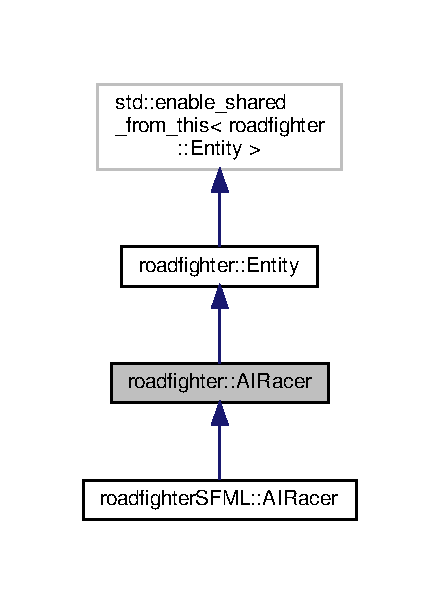
\includegraphics[width=211pt]{classroadfighter_1_1AIRacer__inherit__graph}
\end{center}
\end{figure}


Collaboration diagram for roadfighter\+:\+:A\+I\+Racer\+:\nopagebreak
\begin{figure}[H]
\begin{center}
\leavevmode
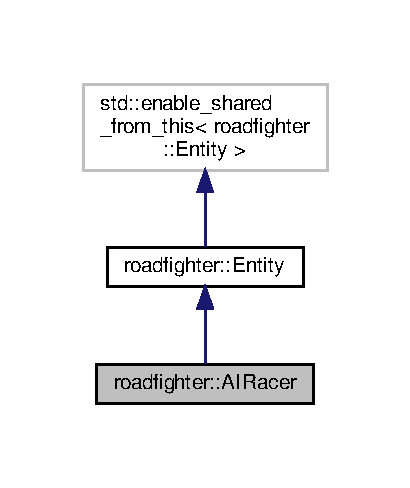
\includegraphics[width=197pt]{classroadfighter_1_1AIRacer__coll__graph}
\end{center}
\end{figure}
\subsection*{Public Member Functions}
\begin{DoxyCompactItemize}
\item 
\hyperlink{classroadfighter_1_1AIRacer_a81234077ec46f9824600f3aeb853d4d1}{A\+I\+Racer} (std\+::shared\+\_\+ptr$<$ \hyperlink{classConfigData}{Config\+Data} $>$ config)
\item 
void \hyperlink{classroadfighter_1_1AIRacer_ab6156385195b3d40d44360d40aafa3a6}{update} (int \hyperlink{classroadfighter_1_1AIRacer_a37f6706ba77522ae4efe782da0125062}{speed}, std\+::shared\+\_\+ptr$<$ \hyperlink{classroadfighter_1_1Entity}{roadfighter\+::\+Entity} $>$ Player) override
\item 
int \hyperlink{classroadfighter_1_1AIRacer_a4fa90fd500b2e790fb50cc6f1505688f}{get\+Speed} () override
\item 
int \hyperlink{classroadfighter_1_1AIRacer_af6fe47885c72aeddd02d13e136f4790f}{Delete} () override
\item 
void \hyperlink{classroadfighter_1_1AIRacer_a10823d4a02dbdad6d760020f8cee7afe}{set\+Delete} (int del) override
\item 
bool \hyperlink{classroadfighter_1_1AIRacer_a9e1ce152093bd4f7deb676c443a7851a}{Shoot} () override
\item 
std\+::shared\+\_\+ptr$<$ \hyperlink{structObjBox}{Obj\+Box} $>$ \hyperlink{classroadfighter_1_1AIRacer_a597fa189f88db3ca1534ddf24bb51c22}{get\+Objbox} () override
\item 
void \hyperlink{classroadfighter_1_1AIRacer_a92afd3d1bfcd290d3b012cbfe44d5a77}{update} () override
\item 
void \hyperlink{classroadfighter_1_1AIRacer_a9f80e1203fb9b718d1bd26ffbb562810}{update\+Movement} (std\+::vector$<$ std\+::shared\+\_\+ptr$<$ \hyperlink{classroadfighter_1_1Entity}{roadfighter\+::\+Entity} $>$$>$ passing\+Cars, std\+::vector$<$ std\+::shared\+\_\+ptr$<$ \hyperlink{classroadfighter_1_1Entity}{roadfighter\+::\+Entity} $>$$>$ Moving\+Cars, std\+::vector$<$ std\+::shared\+\_\+ptr$<$ \hyperlink{classroadfighter_1_1Entity}{roadfighter\+::\+Entity} $>$$>$ Rocks, std\+::shared\+\_\+ptr$<$ \hyperlink{classroadfighter_1_1Entity}{roadfighter\+::\+Entity} $>$ player)
\item 
int \hyperlink{classroadfighter_1_1AIRacer_a74314c736ef3c26fb695a2bdf75bcd31}{get\+Car\+Travelled\+Distance} () const
\end{DoxyCompactItemize}
\subsection*{Protected Attributes}
\begin{DoxyCompactItemize}
\item 
double \hyperlink{classroadfighter_1_1AIRacer_ae05aeeb75376978119b8dacb3a1416a9}{height}
\item 
double \hyperlink{classroadfighter_1_1AIRacer_afb07abbbb10e4d80202390fd940155b1}{width}
\item 
std\+::pair$<$ double, double $>$ \hyperlink{classroadfighter_1_1AIRacer_a3acb0b4859882716e2d1f2732b21a76e}{centralpos} = \{-\/1.\+3, -\/2\}
\item 
int \hyperlink{classroadfighter_1_1AIRacer_a37f6706ba77522ae4efe782da0125062}{speed} = 0
\item 
int \hyperlink{classroadfighter_1_1AIRacer_a7cfbfadf56859ab7865dd080376471c0}{to\+Del} = 0
\item 
int \hyperlink{classroadfighter_1_1AIRacer_a789b1e673e527b791854fe63dce6a963}{Car\+Travelled\+Distance} = 0
\item 
int \hyperlink{classroadfighter_1_1AIRacer_a6b68bb16afb117fce192974c3c044493}{respawntimer}
\item 
int \hyperlink{classroadfighter_1_1AIRacer_af072697ba6c72e186fe67a197caf2783}{respawntime\+Val}
\item 
bool \hyperlink{classroadfighter_1_1AIRacer_a5e5286d19035bc286ef10615bb512dd2}{disable\+Actions} = false
\item 
bool \hyperlink{classroadfighter_1_1AIRacer_a67ebabb7866c75cd75568e1e416c53c9}{finished} = false
\item 
int \hyperlink{classroadfighter_1_1AIRacer_ac997e50a6d864a1bbd4c513748f92836}{maxspeed}
\item 
int \hyperlink{classroadfighter_1_1AIRacer_a2e427cf40da5bde2d5aa30406bb649e1}{acceleration}
\item 
double \hyperlink{classroadfighter_1_1AIRacer_a79095fd3559c3930d6433ea2d92c35b9}{sidemovement} = 0
\end{DoxyCompactItemize}


\subsection{Detailed Description}
Class that handles the AI that moves based on other obstacles and races against the player 

\subsection{Constructor \& Destructor Documentation}
\mbox{\Hypertarget{classroadfighter_1_1AIRacer_a81234077ec46f9824600f3aeb853d4d1}\label{classroadfighter_1_1AIRacer_a81234077ec46f9824600f3aeb853d4d1}} 
\index{roadfighter\+::\+A\+I\+Racer@{roadfighter\+::\+A\+I\+Racer}!A\+I\+Racer@{A\+I\+Racer}}
\index{A\+I\+Racer@{A\+I\+Racer}!roadfighter\+::\+A\+I\+Racer@{roadfighter\+::\+A\+I\+Racer}}
\subsubsection{\texorpdfstring{A\+I\+Racer()}{AIRacer()}}
{\footnotesize\ttfamily roadfighter\+::\+A\+I\+Racer\+::\+A\+I\+Racer (\begin{DoxyParamCaption}\item[{std\+::shared\+\_\+ptr$<$ \hyperlink{classConfigData}{Config\+Data} $>$}]{config }\end{DoxyParamCaption})}

Constructor with the configuration data 
\begin{DoxyParams}{Parameters}
{\em config} & \\
\hline
\end{DoxyParams}


\subsection{Member Function Documentation}
\mbox{\Hypertarget{classroadfighter_1_1AIRacer_af6fe47885c72aeddd02d13e136f4790f}\label{classroadfighter_1_1AIRacer_af6fe47885c72aeddd02d13e136f4790f}} 
\index{roadfighter\+::\+A\+I\+Racer@{roadfighter\+::\+A\+I\+Racer}!Delete@{Delete}}
\index{Delete@{Delete}!roadfighter\+::\+A\+I\+Racer@{roadfighter\+::\+A\+I\+Racer}}
\subsubsection{\texorpdfstring{Delete()}{Delete()}}
{\footnotesize\ttfamily int roadfighter\+::\+A\+I\+Racer\+::\+Delete (\begin{DoxyParamCaption}{ }\end{DoxyParamCaption})\hspace{0.3cm}{\ttfamily [override]}, {\ttfamily [virtual]}}

Returns a certain value to determine the delete status 0 = nothing, 1 = delete, 2 = respawn \begin{DoxyReturn}{Returns}

\end{DoxyReturn}


Implements \hyperlink{classroadfighter_1_1Entity_a08190b0b8e6a3fcdb42273d6096152ac}{roadfighter\+::\+Entity}.

\mbox{\Hypertarget{classroadfighter_1_1AIRacer_a74314c736ef3c26fb695a2bdf75bcd31}\label{classroadfighter_1_1AIRacer_a74314c736ef3c26fb695a2bdf75bcd31}} 
\index{roadfighter\+::\+A\+I\+Racer@{roadfighter\+::\+A\+I\+Racer}!get\+Car\+Travelled\+Distance@{get\+Car\+Travelled\+Distance}}
\index{get\+Car\+Travelled\+Distance@{get\+Car\+Travelled\+Distance}!roadfighter\+::\+A\+I\+Racer@{roadfighter\+::\+A\+I\+Racer}}
\subsubsection{\texorpdfstring{get\+Car\+Travelled\+Distance()}{getCarTravelledDistance()}}
{\footnotesize\ttfamily int roadfighter\+::\+A\+I\+Racer\+::get\+Car\+Travelled\+Distance (\begin{DoxyParamCaption}{ }\end{DoxyParamCaption}) const}

Return the distance the AI has travelled \begin{DoxyReturn}{Returns}

\end{DoxyReturn}
\mbox{\Hypertarget{classroadfighter_1_1AIRacer_a597fa189f88db3ca1534ddf24bb51c22}\label{classroadfighter_1_1AIRacer_a597fa189f88db3ca1534ddf24bb51c22}} 
\index{roadfighter\+::\+A\+I\+Racer@{roadfighter\+::\+A\+I\+Racer}!get\+Objbox@{get\+Objbox}}
\index{get\+Objbox@{get\+Objbox}!roadfighter\+::\+A\+I\+Racer@{roadfighter\+::\+A\+I\+Racer}}
\subsubsection{\texorpdfstring{get\+Objbox()}{getObjbox()}}
{\footnotesize\ttfamily std\+::shared\+\_\+ptr$<$ \hyperlink{structObjBox}{Obj\+Box} $>$ roadfighter\+::\+A\+I\+Racer\+::get\+Objbox (\begin{DoxyParamCaption}{ }\end{DoxyParamCaption})\hspace{0.3cm}{\ttfamily [override]}, {\ttfamily [virtual]}}

Return the object box of the object \begin{DoxyReturn}{Returns}

\end{DoxyReturn}


Implements \hyperlink{classroadfighter_1_1Entity_af14340d04a725175a6d221f23c35fa0c}{roadfighter\+::\+Entity}.

\mbox{\Hypertarget{classroadfighter_1_1AIRacer_a4fa90fd500b2e790fb50cc6f1505688f}\label{classroadfighter_1_1AIRacer_a4fa90fd500b2e790fb50cc6f1505688f}} 
\index{roadfighter\+::\+A\+I\+Racer@{roadfighter\+::\+A\+I\+Racer}!get\+Speed@{get\+Speed}}
\index{get\+Speed@{get\+Speed}!roadfighter\+::\+A\+I\+Racer@{roadfighter\+::\+A\+I\+Racer}}
\subsubsection{\texorpdfstring{get\+Speed()}{getSpeed()}}
{\footnotesize\ttfamily int roadfighter\+::\+A\+I\+Racer\+::get\+Speed (\begin{DoxyParamCaption}{ }\end{DoxyParamCaption})\hspace{0.3cm}{\ttfamily [override]}, {\ttfamily [virtual]}}

Returns the speed of the object \begin{DoxyReturn}{Returns}
speed 
\end{DoxyReturn}


Implements \hyperlink{classroadfighter_1_1Entity_ad3760184d764a61922e1db7d98501ee4}{roadfighter\+::\+Entity}.

\mbox{\Hypertarget{classroadfighter_1_1AIRacer_a10823d4a02dbdad6d760020f8cee7afe}\label{classroadfighter_1_1AIRacer_a10823d4a02dbdad6d760020f8cee7afe}} 
\index{roadfighter\+::\+A\+I\+Racer@{roadfighter\+::\+A\+I\+Racer}!set\+Delete@{set\+Delete}}
\index{set\+Delete@{set\+Delete}!roadfighter\+::\+A\+I\+Racer@{roadfighter\+::\+A\+I\+Racer}}
\subsubsection{\texorpdfstring{set\+Delete()}{setDelete()}}
{\footnotesize\ttfamily void roadfighter\+::\+A\+I\+Racer\+::set\+Delete (\begin{DoxyParamCaption}\item[{int}]{del }\end{DoxyParamCaption})\hspace{0.3cm}{\ttfamily [override]}, {\ttfamily [virtual]}}

Set the delete variable to a certain value 
\begin{DoxyParams}{Parameters}
{\em del} & \\
\hline
\end{DoxyParams}


Implements \hyperlink{classroadfighter_1_1Entity_a07e973f0fa941a69e749629716877692}{roadfighter\+::\+Entity}.

\mbox{\Hypertarget{classroadfighter_1_1AIRacer_a9e1ce152093bd4f7deb676c443a7851a}\label{classroadfighter_1_1AIRacer_a9e1ce152093bd4f7deb676c443a7851a}} 
\index{roadfighter\+::\+A\+I\+Racer@{roadfighter\+::\+A\+I\+Racer}!Shoot@{Shoot}}
\index{Shoot@{Shoot}!roadfighter\+::\+A\+I\+Racer@{roadfighter\+::\+A\+I\+Racer}}
\subsubsection{\texorpdfstring{Shoot()}{Shoot()}}
{\footnotesize\ttfamily bool roadfighter\+::\+A\+I\+Racer\+::\+Shoot (\begin{DoxyParamCaption}{ }\end{DoxyParamCaption})\hspace{0.3cm}{\ttfamily [override]}, {\ttfamily [virtual]}}

Returns if we need to shoot but this function is only used for the player so returns false \begin{DoxyReturn}{Returns}

\end{DoxyReturn}


Implements \hyperlink{classroadfighter_1_1Entity_ad0ecaa0539db252e591da83814251509}{roadfighter\+::\+Entity}.

\mbox{\Hypertarget{classroadfighter_1_1AIRacer_ab6156385195b3d40d44360d40aafa3a6}\label{classroadfighter_1_1AIRacer_ab6156385195b3d40d44360d40aafa3a6}} 
\index{roadfighter\+::\+A\+I\+Racer@{roadfighter\+::\+A\+I\+Racer}!update@{update}}
\index{update@{update}!roadfighter\+::\+A\+I\+Racer@{roadfighter\+::\+A\+I\+Racer}}
\subsubsection{\texorpdfstring{update()}{update()}\hspace{0.1cm}{\footnotesize\ttfamily [1/2]}}
{\footnotesize\ttfamily void roadfighter\+::\+A\+I\+Racer\+::update (\begin{DoxyParamCaption}\item[{int}]{speed,  }\item[{std\+::shared\+\_\+ptr$<$ \hyperlink{classroadfighter_1_1Entity}{roadfighter\+::\+Entity} $>$}]{Player }\end{DoxyParamCaption})\hspace{0.3cm}{\ttfamily [override]}, {\ttfamily [virtual]}}

Update function from the entity with parameters which is not used in this class but has to be specified because it is pure virtual in entity 
\begin{DoxyParams}{Parameters}
{\em speed} & \\
\hline
{\em Player} & \\
\hline
\end{DoxyParams}


Implements \hyperlink{classroadfighter_1_1Entity_a611ba56595dd2137d308876ba820cc09}{roadfighter\+::\+Entity}.

\mbox{\Hypertarget{classroadfighter_1_1AIRacer_a92afd3d1bfcd290d3b012cbfe44d5a77}\label{classroadfighter_1_1AIRacer_a92afd3d1bfcd290d3b012cbfe44d5a77}} 
\index{roadfighter\+::\+A\+I\+Racer@{roadfighter\+::\+A\+I\+Racer}!update@{update}}
\index{update@{update}!roadfighter\+::\+A\+I\+Racer@{roadfighter\+::\+A\+I\+Racer}}
\subsubsection{\texorpdfstring{update()}{update()}\hspace{0.1cm}{\footnotesize\ttfamily [2/2]}}
{\footnotesize\ttfamily void roadfighter\+::\+A\+I\+Racer\+::update (\begin{DoxyParamCaption}{ }\end{DoxyParamCaption})\hspace{0.3cm}{\ttfamily [override]}, {\ttfamily [virtual]}}

Updates the object without parameters Checks when the ai has passed the finish and also controls the respawn timer 

Implements \hyperlink{classroadfighter_1_1Entity_a19cd353f12a3e8432acd6d5609137561}{roadfighter\+::\+Entity}.



Reimplemented in \hyperlink{classroadfighterSFML_1_1AIRacer_aaecd91860a2ac61ef671000e311b7860}{roadfighter\+S\+F\+M\+L\+::\+A\+I\+Racer}.

\mbox{\Hypertarget{classroadfighter_1_1AIRacer_a9f80e1203fb9b718d1bd26ffbb562810}\label{classroadfighter_1_1AIRacer_a9f80e1203fb9b718d1bd26ffbb562810}} 
\index{roadfighter\+::\+A\+I\+Racer@{roadfighter\+::\+A\+I\+Racer}!update\+Movement@{update\+Movement}}
\index{update\+Movement@{update\+Movement}!roadfighter\+::\+A\+I\+Racer@{roadfighter\+::\+A\+I\+Racer}}
\subsubsection{\texorpdfstring{update\+Movement()}{updateMovement()}}
{\footnotesize\ttfamily void roadfighter\+::\+A\+I\+Racer\+::update\+Movement (\begin{DoxyParamCaption}\item[{std\+::vector$<$ std\+::shared\+\_\+ptr$<$ \hyperlink{classroadfighter_1_1Entity}{roadfighter\+::\+Entity} $>$$>$}]{passing\+Cars,  }\item[{std\+::vector$<$ std\+::shared\+\_\+ptr$<$ \hyperlink{classroadfighter_1_1Entity}{roadfighter\+::\+Entity} $>$$>$}]{Moving\+Cars,  }\item[{std\+::vector$<$ std\+::shared\+\_\+ptr$<$ \hyperlink{classroadfighter_1_1Entity}{roadfighter\+::\+Entity} $>$$>$}]{Rocks,  }\item[{std\+::shared\+\_\+ptr$<$ \hyperlink{classroadfighter_1_1Entity}{roadfighter\+::\+Entity} $>$}]{player }\end{DoxyParamCaption})}

Updates the movement of the ai based on the other obstacles in the game it takes the object closest to the front of the car and then moves accordingly Also updates the speed of the AI 
\begin{DoxyParams}{Parameters}
{\em passing\+Cars} & \\
\hline
{\em Moving\+Cars} & \\
\hline
{\em Rocks} & \\
\hline
{\em player} & \\
\hline
\end{DoxyParams}


\subsection{Member Data Documentation}
\mbox{\Hypertarget{classroadfighter_1_1AIRacer_a2e427cf40da5bde2d5aa30406bb649e1}\label{classroadfighter_1_1AIRacer_a2e427cf40da5bde2d5aa30406bb649e1}} 
\index{roadfighter\+::\+A\+I\+Racer@{roadfighter\+::\+A\+I\+Racer}!acceleration@{acceleration}}
\index{acceleration@{acceleration}!roadfighter\+::\+A\+I\+Racer@{roadfighter\+::\+A\+I\+Racer}}
\subsubsection{\texorpdfstring{acceleration}{acceleration}}
{\footnotesize\ttfamily int roadfighter\+::\+A\+I\+Racer\+::acceleration\hspace{0.3cm}{\ttfamily [protected]}}

Maximum speed of the object \mbox{\Hypertarget{classroadfighter_1_1AIRacer_a789b1e673e527b791854fe63dce6a963}\label{classroadfighter_1_1AIRacer_a789b1e673e527b791854fe63dce6a963}} 
\index{roadfighter\+::\+A\+I\+Racer@{roadfighter\+::\+A\+I\+Racer}!Car\+Travelled\+Distance@{Car\+Travelled\+Distance}}
\index{Car\+Travelled\+Distance@{Car\+Travelled\+Distance}!roadfighter\+::\+A\+I\+Racer@{roadfighter\+::\+A\+I\+Racer}}
\subsubsection{\texorpdfstring{Car\+Travelled\+Distance}{CarTravelledDistance}}
{\footnotesize\ttfamily int roadfighter\+::\+A\+I\+Racer\+::\+Car\+Travelled\+Distance = 0\hspace{0.3cm}{\ttfamily [protected]}}

Distance that has been travelled by the player \mbox{\Hypertarget{classroadfighter_1_1AIRacer_a3acb0b4859882716e2d1f2732b21a76e}\label{classroadfighter_1_1AIRacer_a3acb0b4859882716e2d1f2732b21a76e}} 
\index{roadfighter\+::\+A\+I\+Racer@{roadfighter\+::\+A\+I\+Racer}!centralpos@{centralpos}}
\index{centralpos@{centralpos}!roadfighter\+::\+A\+I\+Racer@{roadfighter\+::\+A\+I\+Racer}}
\subsubsection{\texorpdfstring{centralpos}{centralpos}}
{\footnotesize\ttfamily std\+::pair$<$double, double$>$ roadfighter\+::\+A\+I\+Racer\+::centralpos = \{-\/1.\+3, -\/2\}\hspace{0.3cm}{\ttfamily [protected]}}

Pair of the doubles that contains the x and y position of the center of the object \mbox{\Hypertarget{classroadfighter_1_1AIRacer_a5e5286d19035bc286ef10615bb512dd2}\label{classroadfighter_1_1AIRacer_a5e5286d19035bc286ef10615bb512dd2}} 
\index{roadfighter\+::\+A\+I\+Racer@{roadfighter\+::\+A\+I\+Racer}!disable\+Actions@{disable\+Actions}}
\index{disable\+Actions@{disable\+Actions}!roadfighter\+::\+A\+I\+Racer@{roadfighter\+::\+A\+I\+Racer}}
\subsubsection{\texorpdfstring{disable\+Actions}{disableActions}}
{\footnotesize\ttfamily bool roadfighter\+::\+A\+I\+Racer\+::disable\+Actions = false\hspace{0.3cm}{\ttfamily [protected]}}

Boolean that is true when all the action for the ai are disabled \mbox{\Hypertarget{classroadfighter_1_1AIRacer_a67ebabb7866c75cd75568e1e416c53c9}\label{classroadfighter_1_1AIRacer_a67ebabb7866c75cd75568e1e416c53c9}} 
\index{roadfighter\+::\+A\+I\+Racer@{roadfighter\+::\+A\+I\+Racer}!finished@{finished}}
\index{finished@{finished}!roadfighter\+::\+A\+I\+Racer@{roadfighter\+::\+A\+I\+Racer}}
\subsubsection{\texorpdfstring{finished}{finished}}
{\footnotesize\ttfamily bool roadfighter\+::\+A\+I\+Racer\+::finished = false\hspace{0.3cm}{\ttfamily [protected]}}

Boolean that is true when the AI is finished \mbox{\Hypertarget{classroadfighter_1_1AIRacer_ae05aeeb75376978119b8dacb3a1416a9}\label{classroadfighter_1_1AIRacer_ae05aeeb75376978119b8dacb3a1416a9}} 
\index{roadfighter\+::\+A\+I\+Racer@{roadfighter\+::\+A\+I\+Racer}!height@{height}}
\index{height@{height}!roadfighter\+::\+A\+I\+Racer@{roadfighter\+::\+A\+I\+Racer}}
\subsubsection{\texorpdfstring{height}{height}}
{\footnotesize\ttfamily double roadfighter\+::\+A\+I\+Racer\+::height\hspace{0.3cm}{\ttfamily [protected]}}

Height of the object \mbox{\Hypertarget{classroadfighter_1_1AIRacer_ac997e50a6d864a1bbd4c513748f92836}\label{classroadfighter_1_1AIRacer_ac997e50a6d864a1bbd4c513748f92836}} 
\index{roadfighter\+::\+A\+I\+Racer@{roadfighter\+::\+A\+I\+Racer}!maxspeed@{maxspeed}}
\index{maxspeed@{maxspeed}!roadfighter\+::\+A\+I\+Racer@{roadfighter\+::\+A\+I\+Racer}}
\subsubsection{\texorpdfstring{maxspeed}{maxspeed}}
{\footnotesize\ttfamily int roadfighter\+::\+A\+I\+Racer\+::maxspeed\hspace{0.3cm}{\ttfamily [protected]}}

Maximum speed of the object \mbox{\Hypertarget{classroadfighter_1_1AIRacer_a6b68bb16afb117fce192974c3c044493}\label{classroadfighter_1_1AIRacer_a6b68bb16afb117fce192974c3c044493}} 
\index{roadfighter\+::\+A\+I\+Racer@{roadfighter\+::\+A\+I\+Racer}!respawntimer@{respawntimer}}
\index{respawntimer@{respawntimer}!roadfighter\+::\+A\+I\+Racer@{roadfighter\+::\+A\+I\+Racer}}
\subsubsection{\texorpdfstring{respawntimer}{respawntimer}}
{\footnotesize\ttfamily int roadfighter\+::\+A\+I\+Racer\+::respawntimer\hspace{0.3cm}{\ttfamily [protected]}}

Timer for respawning \mbox{\Hypertarget{classroadfighter_1_1AIRacer_af072697ba6c72e186fe67a197caf2783}\label{classroadfighter_1_1AIRacer_af072697ba6c72e186fe67a197caf2783}} 
\index{roadfighter\+::\+A\+I\+Racer@{roadfighter\+::\+A\+I\+Racer}!respawntime\+Val@{respawntime\+Val}}
\index{respawntime\+Val@{respawntime\+Val}!roadfighter\+::\+A\+I\+Racer@{roadfighter\+::\+A\+I\+Racer}}
\subsubsection{\texorpdfstring{respawntime\+Val}{respawntimeVal}}
{\footnotesize\ttfamily int roadfighter\+::\+A\+I\+Racer\+::respawntime\+Val\hspace{0.3cm}{\ttfamily [protected]}}

Value the respawn timer starts at \mbox{\Hypertarget{classroadfighter_1_1AIRacer_a79095fd3559c3930d6433ea2d92c35b9}\label{classroadfighter_1_1AIRacer_a79095fd3559c3930d6433ea2d92c35b9}} 
\index{roadfighter\+::\+A\+I\+Racer@{roadfighter\+::\+A\+I\+Racer}!sidemovement@{sidemovement}}
\index{sidemovement@{sidemovement}!roadfighter\+::\+A\+I\+Racer@{roadfighter\+::\+A\+I\+Racer}}
\subsubsection{\texorpdfstring{sidemovement}{sidemovement}}
{\footnotesize\ttfamily double roadfighter\+::\+A\+I\+Racer\+::sidemovement = 0\hspace{0.3cm}{\ttfamily [protected]}}

Movement the AI has done sideways to control it doesn\textquotesingle{}t keep moving in one direction \mbox{\Hypertarget{classroadfighter_1_1AIRacer_a37f6706ba77522ae4efe782da0125062}\label{classroadfighter_1_1AIRacer_a37f6706ba77522ae4efe782da0125062}} 
\index{roadfighter\+::\+A\+I\+Racer@{roadfighter\+::\+A\+I\+Racer}!speed@{speed}}
\index{speed@{speed}!roadfighter\+::\+A\+I\+Racer@{roadfighter\+::\+A\+I\+Racer}}
\subsubsection{\texorpdfstring{speed}{speed}}
{\footnotesize\ttfamily int roadfighter\+::\+A\+I\+Racer\+::speed = 0\hspace{0.3cm}{\ttfamily [protected]}}

Speed of the object \mbox{\Hypertarget{classroadfighter_1_1AIRacer_a7cfbfadf56859ab7865dd080376471c0}\label{classroadfighter_1_1AIRacer_a7cfbfadf56859ab7865dd080376471c0}} 
\index{roadfighter\+::\+A\+I\+Racer@{roadfighter\+::\+A\+I\+Racer}!to\+Del@{to\+Del}}
\index{to\+Del@{to\+Del}!roadfighter\+::\+A\+I\+Racer@{roadfighter\+::\+A\+I\+Racer}}
\subsubsection{\texorpdfstring{to\+Del}{toDel}}
{\footnotesize\ttfamily int roadfighter\+::\+A\+I\+Racer\+::to\+Del = 0\hspace{0.3cm}{\ttfamily [protected]}}

Object deletion status ( 0 = nothing, 1 = delete, 2 = respawn ) \mbox{\Hypertarget{classroadfighter_1_1AIRacer_afb07abbbb10e4d80202390fd940155b1}\label{classroadfighter_1_1AIRacer_afb07abbbb10e4d80202390fd940155b1}} 
\index{roadfighter\+::\+A\+I\+Racer@{roadfighter\+::\+A\+I\+Racer}!width@{width}}
\index{width@{width}!roadfighter\+::\+A\+I\+Racer@{roadfighter\+::\+A\+I\+Racer}}
\subsubsection{\texorpdfstring{width}{width}}
{\footnotesize\ttfamily double roadfighter\+::\+A\+I\+Racer\+::width\hspace{0.3cm}{\ttfamily [protected]}}

Width of the object 

The documentation for this class was generated from the following files\+:\begin{DoxyCompactItemize}
\item 
roadfighter/A\+I\+Racer.\+h\item 
roadfighter/A\+I\+Racer.\+cpp\end{DoxyCompactItemize}

\hypertarget{classroadfighterSFML_1_1AIRacer}{}\section{roadfighter\+S\+F\+ML\+:\+:A\+I\+Racer Class Reference}
\label{classroadfighterSFML_1_1AIRacer}\index{roadfighter\+S\+F\+M\+L\+::\+A\+I\+Racer@{roadfighter\+S\+F\+M\+L\+::\+A\+I\+Racer}}


{\ttfamily \#include $<$A\+I\+Racer.\+h$>$}



Inheritance diagram for roadfighter\+S\+F\+ML\+:\+:A\+I\+Racer\+:\nopagebreak
\begin{figure}[H]
\begin{center}
\leavevmode
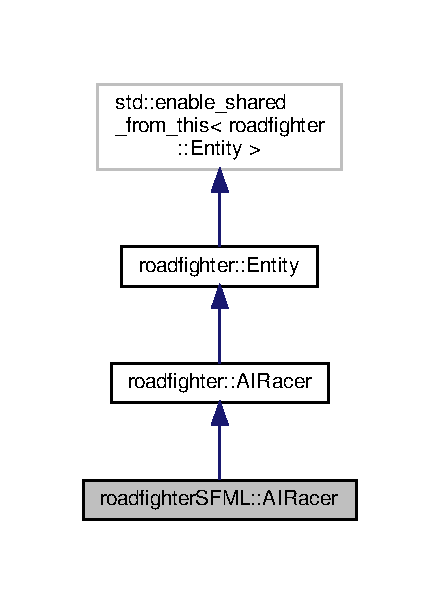
\includegraphics[width=211pt]{classroadfighterSFML_1_1AIRacer__inherit__graph}
\end{center}
\end{figure}


Collaboration diagram for roadfighter\+S\+F\+ML\+:\+:A\+I\+Racer\+:\nopagebreak
\begin{figure}[H]
\begin{center}
\leavevmode
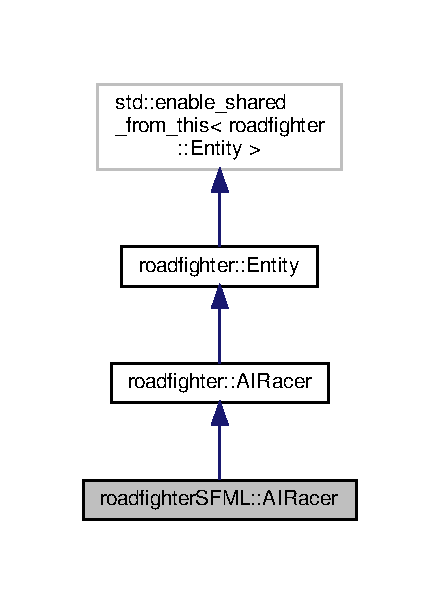
\includegraphics[width=211pt]{classroadfighterSFML_1_1AIRacer__coll__graph}
\end{center}
\end{figure}
\subsection*{Public Member Functions}
\begin{DoxyCompactItemize}
\item 
\hyperlink{classroadfighterSFML_1_1AIRacer_a357c65d57f1560a4c0d00da98820578b}{A\+I\+Racer} (const std\+::shared\+\_\+ptr$<$ sf\+::\+Render\+Window $>$ window, std\+::shared\+\_\+ptr$<$ \hyperlink{classConfigData}{Config\+Data} $>$ config)
\item 
void \hyperlink{classroadfighterSFML_1_1AIRacer_a50d966c9d59e09a155d69e2c2296fb4e}{draw} () override
\item 
void \hyperlink{classroadfighterSFML_1_1AIRacer_aaecd91860a2ac61ef671000e311b7860}{update} () override
\end{DoxyCompactItemize}
\subsection*{Additional Inherited Members}


\subsection{Detailed Description}
Graphic side of the AI 

\subsection{Constructor \& Destructor Documentation}
\mbox{\Hypertarget{classroadfighterSFML_1_1AIRacer_a357c65d57f1560a4c0d00da98820578b}\label{classroadfighterSFML_1_1AIRacer_a357c65d57f1560a4c0d00da98820578b}} 
\index{roadfighter\+S\+F\+M\+L\+::\+A\+I\+Racer@{roadfighter\+S\+F\+M\+L\+::\+A\+I\+Racer}!A\+I\+Racer@{A\+I\+Racer}}
\index{A\+I\+Racer@{A\+I\+Racer}!roadfighter\+S\+F\+M\+L\+::\+A\+I\+Racer@{roadfighter\+S\+F\+M\+L\+::\+A\+I\+Racer}}
\subsubsection{\texorpdfstring{A\+I\+Racer()}{AIRacer()}}
{\footnotesize\ttfamily roadfighter\+S\+F\+M\+L\+::\+A\+I\+Racer\+::\+A\+I\+Racer (\begin{DoxyParamCaption}\item[{const std\+::shared\+\_\+ptr$<$ sf\+::\+Render\+Window $>$}]{window,  }\item[{std\+::shared\+\_\+ptr$<$ \hyperlink{classConfigData}{Config\+Data} $>$}]{config }\end{DoxyParamCaption})}

Constructor with sfml window and configuration data 
\begin{DoxyParams}{Parameters}
{\em window} & \\
\hline
{\em config} & \\
\hline
\end{DoxyParams}


\subsection{Member Function Documentation}
\mbox{\Hypertarget{classroadfighterSFML_1_1AIRacer_a50d966c9d59e09a155d69e2c2296fb4e}\label{classroadfighterSFML_1_1AIRacer_a50d966c9d59e09a155d69e2c2296fb4e}} 
\index{roadfighter\+S\+F\+M\+L\+::\+A\+I\+Racer@{roadfighter\+S\+F\+M\+L\+::\+A\+I\+Racer}!draw@{draw}}
\index{draw@{draw}!roadfighter\+S\+F\+M\+L\+::\+A\+I\+Racer@{roadfighter\+S\+F\+M\+L\+::\+A\+I\+Racer}}
\subsubsection{\texorpdfstring{draw()}{draw()}}
{\footnotesize\ttfamily void roadfighter\+S\+F\+M\+L\+::\+A\+I\+Racer\+::draw (\begin{DoxyParamCaption}{ }\end{DoxyParamCaption})\hspace{0.3cm}{\ttfamily [override]}, {\ttfamily [virtual]}}

Draws the player 

Implements \hyperlink{classroadfighter_1_1Entity_ac516f8005f969ad5a86c252e5a3640ee}{roadfighter\+::\+Entity}.

\mbox{\Hypertarget{classroadfighterSFML_1_1AIRacer_aaecd91860a2ac61ef671000e311b7860}\label{classroadfighterSFML_1_1AIRacer_aaecd91860a2ac61ef671000e311b7860}} 
\index{roadfighter\+S\+F\+M\+L\+::\+A\+I\+Racer@{roadfighter\+S\+F\+M\+L\+::\+A\+I\+Racer}!update@{update}}
\index{update@{update}!roadfighter\+S\+F\+M\+L\+::\+A\+I\+Racer@{roadfighter\+S\+F\+M\+L\+::\+A\+I\+Racer}}
\subsubsection{\texorpdfstring{update()}{update()}}
{\footnotesize\ttfamily void roadfighter\+S\+F\+M\+L\+::\+A\+I\+Racer\+::update (\begin{DoxyParamCaption}{ }\end{DoxyParamCaption})\hspace{0.3cm}{\ttfamily [override]}, {\ttfamily [virtual]}}

Updates the player 

Reimplemented from \hyperlink{classroadfighter_1_1AIRacer_a92afd3d1bfcd290d3b012cbfe44d5a77}{roadfighter\+::\+A\+I\+Racer}.



The documentation for this class was generated from the following files\+:\begin{DoxyCompactItemize}
\item 
roadfighter\+S\+F\+M\+L/A\+I\+Racer.\+h\item 
roadfighter\+S\+F\+M\+L/A\+I\+Racer.\+cpp\end{DoxyCompactItemize}

\hypertarget{classroadfighter_1_1Background}{}\section{roadfighter\+:\+:Background Class Reference}
\label{classroadfighter_1_1Background}\index{roadfighter\+::\+Background@{roadfighter\+::\+Background}}


{\ttfamily \#include $<$Background.\+h$>$}



Inheritance diagram for roadfighter\+:\+:Background\+:\nopagebreak
\begin{figure}[H]
\begin{center}
\leavevmode
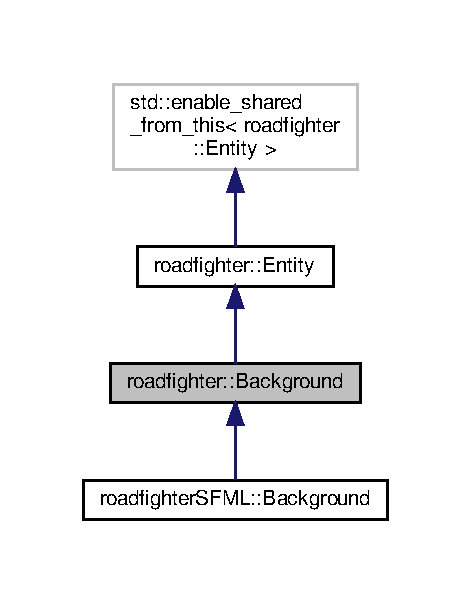
\includegraphics[width=226pt]{classroadfighter_1_1Background__inherit__graph}
\end{center}
\end{figure}


Collaboration diagram for roadfighter\+:\+:Background\+:\nopagebreak
\begin{figure}[H]
\begin{center}
\leavevmode
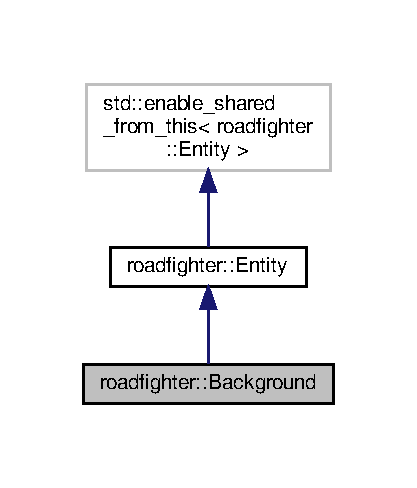
\includegraphics[width=200pt]{classroadfighter_1_1Background__coll__graph}
\end{center}
\end{figure}
\subsection*{Public Member Functions}
\begin{DoxyCompactItemize}
\item 
\hyperlink{classroadfighter_1_1Background_a7b01984ecdbd0ec7e2d2d9962463f663}{Background} (std\+::shared\+\_\+ptr$<$ \hyperlink{classConfigData}{Config\+Data} $>$ config)
\item 
void \hyperlink{classroadfighter_1_1Background_a6fa762ca6aa2f18918c1b715ae94395f}{update} () override
\item 
void \hyperlink{classroadfighter_1_1Background_a881ed4d9e98e86ce7128c0fd18f82160}{update} (int speed, std\+::shared\+\_\+ptr$<$ \hyperlink{classroadfighter_1_1Entity}{roadfighter\+::\+Entity} $>$ Player) override
\item 
int \hyperlink{classroadfighter_1_1Background_acbeaa8438617d67f8069347000e185a1}{get\+Speed} () override
\item 
int \hyperlink{classroadfighter_1_1Background_a6541d509079dfa940d9f7ec2ab706963}{Delete} () override
\item 
std\+::shared\+\_\+ptr$<$ \hyperlink{structObjBox}{Obj\+Box} $>$ \hyperlink{classroadfighter_1_1Background_af25322839a52bc232266cceb2a85dd7d}{get\+Objbox} () override
\item 
void \hyperlink{classroadfighter_1_1Background_acb4cdc56872d164b297b5655124df54d}{set\+Delete} (int del) override
\item 
bool \hyperlink{classroadfighter_1_1Background_a1482152bca4207b44f1ce1c2c5af5847}{Shoot} () override
\end{DoxyCompactItemize}
\subsection*{Protected Attributes}
\begin{DoxyCompactItemize}
\item 
std\+::pair$<$ double, double $>$ \hyperlink{classroadfighter_1_1Background_a490223cc4c2fe332df45506a26bc48ba}{centralpos1} = \{-\/1, -\/3\}
\item 
std\+::pair$<$ double, double $>$ \hyperlink{classroadfighter_1_1Background_a5acc0e95972469cf195057e862e88b1a}{centralpos2} = \{-\/1, 3\}
\item 
std\+::pair$<$ double, double $>$ \hyperlink{classroadfighter_1_1Background_a756bfd2a4af29498e9796b73cde5cbf3}{centralpos3} = \{-\/1, 9\}
\item 
std\+::pair$<$ double, double $>$ \hyperlink{classroadfighter_1_1Background_a63c941e322b2f9113c61c1d5f07d5912}{centralposfin} = \{-\/1, 3\}
\item 
bool \hyperlink{classroadfighter_1_1Background_a7e8171af25b6b6aadc8a256bf360b351}{move\+Finish} = false
\item 
int \hyperlink{classroadfighter_1_1Background_a90c142a5d66d6e261bf33f6037b4f77d}{to\+Del} = 0
\item 
int \hyperlink{classroadfighter_1_1Background_a084a46a73deb42183773dfd29adbc106}{Car\+Travelled\+Distance} = 0
\end{DoxyCompactItemize}


\subsection{Detailed Description}
Class that moves the background and makes sure it appears infinite 

\subsection{Constructor \& Destructor Documentation}
\mbox{\Hypertarget{classroadfighter_1_1Background_a7b01984ecdbd0ec7e2d2d9962463f663}\label{classroadfighter_1_1Background_a7b01984ecdbd0ec7e2d2d9962463f663}} 
\index{roadfighter\+::\+Background@{roadfighter\+::\+Background}!Background@{Background}}
\index{Background@{Background}!roadfighter\+::\+Background@{roadfighter\+::\+Background}}
\subsubsection{\texorpdfstring{Background()}{Background()}}
{\footnotesize\ttfamily roadfighter\+::\+Background\+::\+Background (\begin{DoxyParamCaption}\item[{std\+::shared\+\_\+ptr$<$ \hyperlink{classConfigData}{Config\+Data} $>$}]{config }\end{DoxyParamCaption})}

Constructor with configuration data 
\begin{DoxyParams}{Parameters}
{\em config} & \\
\hline
\end{DoxyParams}


\subsection{Member Function Documentation}
\mbox{\Hypertarget{classroadfighter_1_1Background_a6541d509079dfa940d9f7ec2ab706963}\label{classroadfighter_1_1Background_a6541d509079dfa940d9f7ec2ab706963}} 
\index{roadfighter\+::\+Background@{roadfighter\+::\+Background}!Delete@{Delete}}
\index{Delete@{Delete}!roadfighter\+::\+Background@{roadfighter\+::\+Background}}
\subsubsection{\texorpdfstring{Delete()}{Delete()}}
{\footnotesize\ttfamily int roadfighter\+::\+Background\+::\+Delete (\begin{DoxyParamCaption}{ }\end{DoxyParamCaption})\hspace{0.3cm}{\ttfamily [override]}, {\ttfamily [virtual]}}

Returns a certain value to determine the delete status 0 = nothing, 1 = delete, 2 = respawn \begin{DoxyReturn}{Returns}

\end{DoxyReturn}


Implements \hyperlink{classroadfighter_1_1Entity_a08190b0b8e6a3fcdb42273d6096152ac}{roadfighter\+::\+Entity}.

\mbox{\Hypertarget{classroadfighter_1_1Background_af25322839a52bc232266cceb2a85dd7d}\label{classroadfighter_1_1Background_af25322839a52bc232266cceb2a85dd7d}} 
\index{roadfighter\+::\+Background@{roadfighter\+::\+Background}!get\+Objbox@{get\+Objbox}}
\index{get\+Objbox@{get\+Objbox}!roadfighter\+::\+Background@{roadfighter\+::\+Background}}
\subsubsection{\texorpdfstring{get\+Objbox()}{getObjbox()}}
{\footnotesize\ttfamily std\+::shared\+\_\+ptr$<$ \hyperlink{structObjBox}{Obj\+Box} $>$ roadfighter\+::\+Background\+::get\+Objbox (\begin{DoxyParamCaption}{ }\end{DoxyParamCaption})\hspace{0.3cm}{\ttfamily [override]}, {\ttfamily [virtual]}}

Return the object box of the object \begin{DoxyReturn}{Returns}

\end{DoxyReturn}


Implements \hyperlink{classroadfighter_1_1Entity_af14340d04a725175a6d221f23c35fa0c}{roadfighter\+::\+Entity}.

\mbox{\Hypertarget{classroadfighter_1_1Background_acbeaa8438617d67f8069347000e185a1}\label{classroadfighter_1_1Background_acbeaa8438617d67f8069347000e185a1}} 
\index{roadfighter\+::\+Background@{roadfighter\+::\+Background}!get\+Speed@{get\+Speed}}
\index{get\+Speed@{get\+Speed}!roadfighter\+::\+Background@{roadfighter\+::\+Background}}
\subsubsection{\texorpdfstring{get\+Speed()}{getSpeed()}}
{\footnotesize\ttfamily int roadfighter\+::\+Background\+::get\+Speed (\begin{DoxyParamCaption}{ }\end{DoxyParamCaption})\hspace{0.3cm}{\ttfamily [override]}, {\ttfamily [virtual]}}

Returns the speed of the object \begin{DoxyReturn}{Returns}
speed 
\end{DoxyReturn}


Implements \hyperlink{classroadfighter_1_1Entity_ad3760184d764a61922e1db7d98501ee4}{roadfighter\+::\+Entity}.

\mbox{\Hypertarget{classroadfighter_1_1Background_acb4cdc56872d164b297b5655124df54d}\label{classroadfighter_1_1Background_acb4cdc56872d164b297b5655124df54d}} 
\index{roadfighter\+::\+Background@{roadfighter\+::\+Background}!set\+Delete@{set\+Delete}}
\index{set\+Delete@{set\+Delete}!roadfighter\+::\+Background@{roadfighter\+::\+Background}}
\subsubsection{\texorpdfstring{set\+Delete()}{setDelete()}}
{\footnotesize\ttfamily void roadfighter\+::\+Background\+::set\+Delete (\begin{DoxyParamCaption}\item[{int}]{del }\end{DoxyParamCaption})\hspace{0.3cm}{\ttfamily [override]}, {\ttfamily [virtual]}}

Sets if the object must be deleted 
\begin{DoxyParams}{Parameters}
{\em del} & \\
\hline
\end{DoxyParams}


Implements \hyperlink{classroadfighter_1_1Entity_a07e973f0fa941a69e749629716877692}{roadfighter\+::\+Entity}.

\mbox{\Hypertarget{classroadfighter_1_1Background_a1482152bca4207b44f1ce1c2c5af5847}\label{classroadfighter_1_1Background_a1482152bca4207b44f1ce1c2c5af5847}} 
\index{roadfighter\+::\+Background@{roadfighter\+::\+Background}!Shoot@{Shoot}}
\index{Shoot@{Shoot}!roadfighter\+::\+Background@{roadfighter\+::\+Background}}
\subsubsection{\texorpdfstring{Shoot()}{Shoot()}}
{\footnotesize\ttfamily bool roadfighter\+::\+Background\+::\+Shoot (\begin{DoxyParamCaption}{ }\end{DoxyParamCaption})\hspace{0.3cm}{\ttfamily [override]}, {\ttfamily [virtual]}}

Return if the object shoots \begin{DoxyReturn}{Returns}

\end{DoxyReturn}


Implements \hyperlink{classroadfighter_1_1Entity_ad0ecaa0539db252e591da83814251509}{roadfighter\+::\+Entity}.

\mbox{\Hypertarget{classroadfighter_1_1Background_a6fa762ca6aa2f18918c1b715ae94395f}\label{classroadfighter_1_1Background_a6fa762ca6aa2f18918c1b715ae94395f}} 
\index{roadfighter\+::\+Background@{roadfighter\+::\+Background}!update@{update}}
\index{update@{update}!roadfighter\+::\+Background@{roadfighter\+::\+Background}}
\subsubsection{\texorpdfstring{update()}{update()}\hspace{0.1cm}{\footnotesize\ttfamily [1/2]}}
{\footnotesize\ttfamily void roadfighter\+::\+Background\+::update (\begin{DoxyParamCaption}{ }\end{DoxyParamCaption})\hspace{0.3cm}{\ttfamily [override]}, {\ttfamily [virtual]}}

Updates the object 

Implements \hyperlink{classroadfighter_1_1Entity_a19cd353f12a3e8432acd6d5609137561}{roadfighter\+::\+Entity}.

\mbox{\Hypertarget{classroadfighter_1_1Background_a881ed4d9e98e86ce7128c0fd18f82160}\label{classroadfighter_1_1Background_a881ed4d9e98e86ce7128c0fd18f82160}} 
\index{roadfighter\+::\+Background@{roadfighter\+::\+Background}!update@{update}}
\index{update@{update}!roadfighter\+::\+Background@{roadfighter\+::\+Background}}
\subsubsection{\texorpdfstring{update()}{update()}\hspace{0.1cm}{\footnotesize\ttfamily [2/2]}}
{\footnotesize\ttfamily void roadfighter\+::\+Background\+::update (\begin{DoxyParamCaption}\item[{int}]{speed,  }\item[{std\+::shared\+\_\+ptr$<$ \hyperlink{classroadfighter_1_1Entity}{roadfighter\+::\+Entity} $>$}]{Player }\end{DoxyParamCaption})\hspace{0.3cm}{\ttfamily [override]}, {\ttfamily [virtual]}}

Updates the object with extra parameters The speed is used to see how much we need to move the backgrounds 
\begin{DoxyParams}{Parameters}
{\em speed} & \\
\hline
{\em Player} & \\
\hline
\end{DoxyParams}


Implements \hyperlink{classroadfighter_1_1Entity_a611ba56595dd2137d308876ba820cc09}{roadfighter\+::\+Entity}.



\subsection{Member Data Documentation}
\mbox{\Hypertarget{classroadfighter_1_1Background_a084a46a73deb42183773dfd29adbc106}\label{classroadfighter_1_1Background_a084a46a73deb42183773dfd29adbc106}} 
\index{roadfighter\+::\+Background@{roadfighter\+::\+Background}!Car\+Travelled\+Distance@{Car\+Travelled\+Distance}}
\index{Car\+Travelled\+Distance@{Car\+Travelled\+Distance}!roadfighter\+::\+Background@{roadfighter\+::\+Background}}
\subsubsection{\texorpdfstring{Car\+Travelled\+Distance}{CarTravelledDistance}}
{\footnotesize\ttfamily int roadfighter\+::\+Background\+::\+Car\+Travelled\+Distance = 0\hspace{0.3cm}{\ttfamily [protected]}}

Distance the car has travelled (to know when to show finish) \mbox{\Hypertarget{classroadfighter_1_1Background_a490223cc4c2fe332df45506a26bc48ba}\label{classroadfighter_1_1Background_a490223cc4c2fe332df45506a26bc48ba}} 
\index{roadfighter\+::\+Background@{roadfighter\+::\+Background}!centralpos1@{centralpos1}}
\index{centralpos1@{centralpos1}!roadfighter\+::\+Background@{roadfighter\+::\+Background}}
\subsubsection{\texorpdfstring{centralpos1}{centralpos1}}
{\footnotesize\ttfamily std\+::pair$<$double, double$>$ roadfighter\+::\+Background\+::centralpos1 = \{-\/1, -\/3\}\hspace{0.3cm}{\ttfamily [protected]}}

X and Y positions of the first background sprite \mbox{\Hypertarget{classroadfighter_1_1Background_a5acc0e95972469cf195057e862e88b1a}\label{classroadfighter_1_1Background_a5acc0e95972469cf195057e862e88b1a}} 
\index{roadfighter\+::\+Background@{roadfighter\+::\+Background}!centralpos2@{centralpos2}}
\index{centralpos2@{centralpos2}!roadfighter\+::\+Background@{roadfighter\+::\+Background}}
\subsubsection{\texorpdfstring{centralpos2}{centralpos2}}
{\footnotesize\ttfamily std\+::pair$<$double, double$>$ roadfighter\+::\+Background\+::centralpos2 = \{-\/1, 3\}\hspace{0.3cm}{\ttfamily [protected]}}

X and Y positions of the second background sprite \mbox{\Hypertarget{classroadfighter_1_1Background_a756bfd2a4af29498e9796b73cde5cbf3}\label{classroadfighter_1_1Background_a756bfd2a4af29498e9796b73cde5cbf3}} 
\index{roadfighter\+::\+Background@{roadfighter\+::\+Background}!centralpos3@{centralpos3}}
\index{centralpos3@{centralpos3}!roadfighter\+::\+Background@{roadfighter\+::\+Background}}
\subsubsection{\texorpdfstring{centralpos3}{centralpos3}}
{\footnotesize\ttfamily std\+::pair$<$double, double$>$ roadfighter\+::\+Background\+::centralpos3 = \{-\/1, 9\}\hspace{0.3cm}{\ttfamily [protected]}}

X and Y positions of the third background sprite \mbox{\Hypertarget{classroadfighter_1_1Background_a63c941e322b2f9113c61c1d5f07d5912}\label{classroadfighter_1_1Background_a63c941e322b2f9113c61c1d5f07d5912}} 
\index{roadfighter\+::\+Background@{roadfighter\+::\+Background}!centralposfin@{centralposfin}}
\index{centralposfin@{centralposfin}!roadfighter\+::\+Background@{roadfighter\+::\+Background}}
\subsubsection{\texorpdfstring{centralposfin}{centralposfin}}
{\footnotesize\ttfamily std\+::pair$<$double, double$>$ roadfighter\+::\+Background\+::centralposfin = \{-\/1, 3\}\hspace{0.3cm}{\ttfamily [protected]}}

X and Y positions of the finish background sprite \mbox{\Hypertarget{classroadfighter_1_1Background_a7e8171af25b6b6aadc8a256bf360b351}\label{classroadfighter_1_1Background_a7e8171af25b6b6aadc8a256bf360b351}} 
\index{roadfighter\+::\+Background@{roadfighter\+::\+Background}!move\+Finish@{move\+Finish}}
\index{move\+Finish@{move\+Finish}!roadfighter\+::\+Background@{roadfighter\+::\+Background}}
\subsubsection{\texorpdfstring{move\+Finish}{moveFinish}}
{\footnotesize\ttfamily bool roadfighter\+::\+Background\+::move\+Finish = false\hspace{0.3cm}{\ttfamily [protected]}}

Boolean that is true if we need to move the finish \mbox{\Hypertarget{classroadfighter_1_1Background_a90c142a5d66d6e261bf33f6037b4f77d}\label{classroadfighter_1_1Background_a90c142a5d66d6e261bf33f6037b4f77d}} 
\index{roadfighter\+::\+Background@{roadfighter\+::\+Background}!to\+Del@{to\+Del}}
\index{to\+Del@{to\+Del}!roadfighter\+::\+Background@{roadfighter\+::\+Background}}
\subsubsection{\texorpdfstring{to\+Del}{toDel}}
{\footnotesize\ttfamily int roadfighter\+::\+Background\+::to\+Del = 0\hspace{0.3cm}{\ttfamily [protected]}}

Object deletion status ( 0 = nothing, 1 = delete, 2 = respawn ) 

The documentation for this class was generated from the following files\+:\begin{DoxyCompactItemize}
\item 
roadfighter/Background.\+h\item 
roadfighter/Background.\+cpp\end{DoxyCompactItemize}

\hypertarget{classroadfighterSFML_1_1Background}{}\section{roadfighter\+S\+F\+ML\+:\+:Background Class Reference}
\label{classroadfighterSFML_1_1Background}\index{roadfighter\+S\+F\+M\+L\+::\+Background@{roadfighter\+S\+F\+M\+L\+::\+Background}}


{\ttfamily \#include $<$Background.\+h$>$}



Inheritance diagram for roadfighter\+S\+F\+ML\+:\+:Background\+:\nopagebreak
\begin{figure}[H]
\begin{center}
\leavevmode
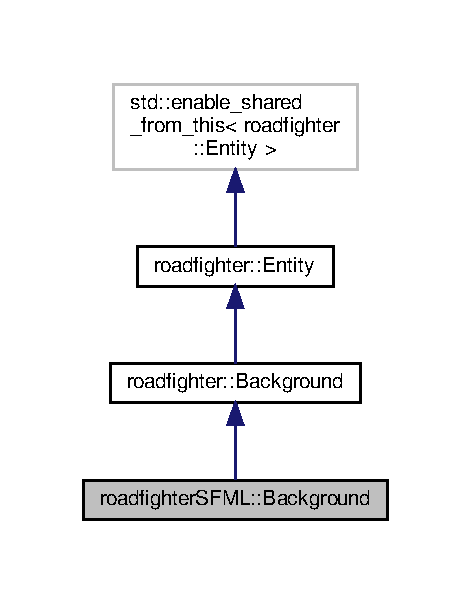
\includegraphics[width=226pt]{classroadfighterSFML_1_1Background__inherit__graph}
\end{center}
\end{figure}


Collaboration diagram for roadfighter\+S\+F\+ML\+:\+:Background\+:\nopagebreak
\begin{figure}[H]
\begin{center}
\leavevmode
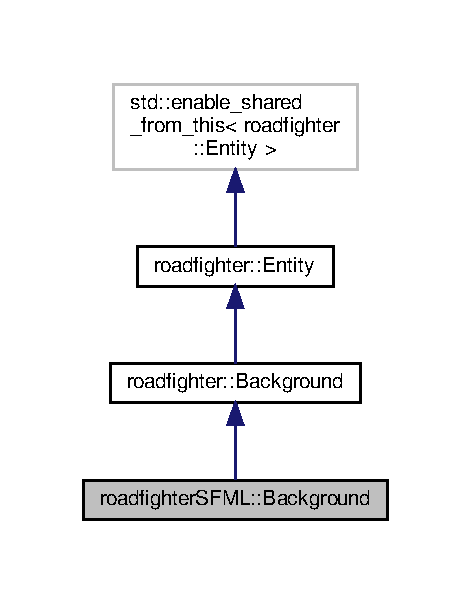
\includegraphics[width=226pt]{classroadfighterSFML_1_1Background__coll__graph}
\end{center}
\end{figure}
\subsection*{Public Member Functions}
\begin{DoxyCompactItemize}
\item 
\hyperlink{classroadfighterSFML_1_1Background_ade9e620ebf8ae9a92012a85c356788b1}{Background} (const std\+::shared\+\_\+ptr$<$ sf\+::\+Render\+Window $>$ \&window, int type, std\+::shared\+\_\+ptr$<$ \hyperlink{classConfigData}{Config\+Data} $>$ config)
\item 
void \hyperlink{classroadfighterSFML_1_1Background_a02b49875cfb5d0c77d30c2ddbc05c46f}{draw} () override
\end{DoxyCompactItemize}
\subsection*{Additional Inherited Members}


\subsection{Detailed Description}
Graphic side of the background 

\subsection{Constructor \& Destructor Documentation}
\mbox{\Hypertarget{classroadfighterSFML_1_1Background_ade9e620ebf8ae9a92012a85c356788b1}\label{classroadfighterSFML_1_1Background_ade9e620ebf8ae9a92012a85c356788b1}} 
\index{roadfighter\+S\+F\+M\+L\+::\+Background@{roadfighter\+S\+F\+M\+L\+::\+Background}!Background@{Background}}
\index{Background@{Background}!roadfighter\+S\+F\+M\+L\+::\+Background@{roadfighter\+S\+F\+M\+L\+::\+Background}}
\subsubsection{\texorpdfstring{Background()}{Background()}}
{\footnotesize\ttfamily roadfighter\+S\+F\+M\+L\+::\+Background\+::\+Background (\begin{DoxyParamCaption}\item[{const std\+::shared\+\_\+ptr$<$ sf\+::\+Render\+Window $>$ \&}]{window,  }\item[{int}]{type,  }\item[{std\+::shared\+\_\+ptr$<$ \hyperlink{classConfigData}{Config\+Data} $>$}]{config }\end{DoxyParamCaption})}

Constructor with sfml level what the level is and configuration data 
\begin{DoxyParams}{Parameters}
{\em window} & \\
\hline
{\em type} & \\
\hline
{\em config} & \\
\hline
\end{DoxyParams}


\subsection{Member Function Documentation}
\mbox{\Hypertarget{classroadfighterSFML_1_1Background_a02b49875cfb5d0c77d30c2ddbc05c46f}\label{classroadfighterSFML_1_1Background_a02b49875cfb5d0c77d30c2ddbc05c46f}} 
\index{roadfighter\+S\+F\+M\+L\+::\+Background@{roadfighter\+S\+F\+M\+L\+::\+Background}!draw@{draw}}
\index{draw@{draw}!roadfighter\+S\+F\+M\+L\+::\+Background@{roadfighter\+S\+F\+M\+L\+::\+Background}}
\subsubsection{\texorpdfstring{draw()}{draw()}}
{\footnotesize\ttfamily void roadfighter\+S\+F\+M\+L\+::\+Background\+::draw (\begin{DoxyParamCaption}{ }\end{DoxyParamCaption})\hspace{0.3cm}{\ttfamily [override]}, {\ttfamily [virtual]}}

Draws the background 

Implements \hyperlink{classroadfighter_1_1Entity_ac516f8005f969ad5a86c252e5a3640ee}{roadfighter\+::\+Entity}.



The documentation for this class was generated from the following files\+:\begin{DoxyCompactItemize}
\item 
roadfighter\+S\+F\+M\+L/Background.\+h\item 
roadfighter\+S\+F\+M\+L/Background.\+cpp\end{DoxyCompactItemize}

\hypertarget{classroadfighter_1_1Boss}{}\section{roadfighter\+:\+:Boss Class Reference}
\label{classroadfighter_1_1Boss}\index{roadfighter\+::\+Boss@{roadfighter\+::\+Boss}}


{\ttfamily \#include $<$Boss.\+h$>$}



Inheritance diagram for roadfighter\+:\+:Boss\+:\nopagebreak
\begin{figure}[H]
\begin{center}
\leavevmode
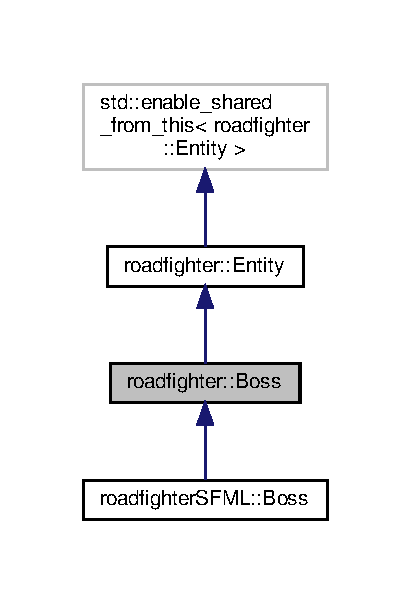
\includegraphics[width=197pt]{classroadfighter_1_1Boss__inherit__graph}
\end{center}
\end{figure}


Collaboration diagram for roadfighter\+:\+:Boss\+:\nopagebreak
\begin{figure}[H]
\begin{center}
\leavevmode
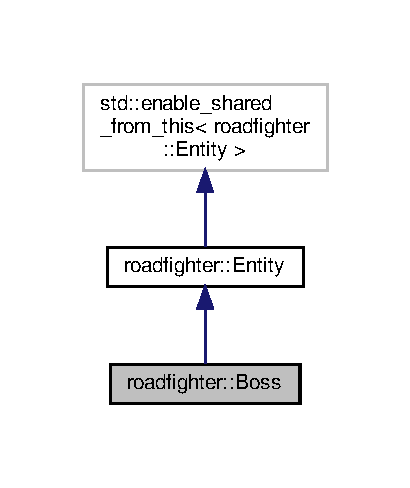
\includegraphics[width=197pt]{classroadfighter_1_1Boss__coll__graph}
\end{center}
\end{figure}
\subsection*{Public Member Functions}
\begin{DoxyCompactItemize}
\item 
\hyperlink{classroadfighter_1_1Boss_ae71359243be30ff532283b15be66bb70}{Boss} (std\+::shared\+\_\+ptr$<$ \hyperlink{classConfigData}{Config\+Data} $>$ config)
\item 
void \hyperlink{classroadfighter_1_1Boss_aa097f1f2e3fe76645233a4ba75ee6256}{update} () override
\item 
void \hyperlink{classroadfighter_1_1Boss_a1754fba639f122f50e3eeb55980008b2}{update} (int speed, std\+::shared\+\_\+ptr$<$ \hyperlink{classroadfighter_1_1Entity}{roadfighter\+::\+Entity} $>$ Player) override
\item 
int \hyperlink{classroadfighter_1_1Boss_a348151aa9aabb3baabf9a8cc0b6955cb}{get\+Speed} () override
\item 
int \hyperlink{classroadfighter_1_1Boss_a8ffadaa85b61447da023c043d3d2dcc9}{Delete} () override
\item 
void \hyperlink{classroadfighter_1_1Boss_a8e2d5737afc0df4bc8b8ad0ddc03f5b8}{set\+Delete} (int del) override
\item 
bool \hyperlink{classroadfighter_1_1Boss_a794027599b17398ae72c65aa1837d864}{Shoot} () override
\item 
std\+::shared\+\_\+ptr$<$ \hyperlink{structObjBox}{Obj\+Box} $>$ \hyperlink{classroadfighter_1_1Boss_a3cf68c683f4352908eab55fc6ee29e9e}{get\+Objbox} () override
\item 
bool \hyperlink{classroadfighter_1_1Boss_a87c3a59c31b8babf464711a69c74622d}{is\+Get\+Rocks} () const
\item 
void \hyperlink{classroadfighter_1_1Boss_a86ef044739f08440f8b63a17f3e60d01}{set\+Get\+Rocks} (bool \hyperlink{classroadfighter_1_1Boss_a276f3388ae889d5b9e32e4e68ecd8e55}{get\+Rocks})
\item 
const std\+::vector$<$ double $>$ \& \hyperlink{classroadfighter_1_1Boss_a9be5ed79ba9419881bb972ea9582b110}{get\+Rock\+Pos} () const
\item 
int \hyperlink{classroadfighter_1_1Boss_a06a715dad575e6e51f78be8c8c0836f7}{get\+Life} () const
\item 
void \hyperlink{classroadfighter_1_1Boss_a170c46fc7f03d6e59633c370c6fd478c}{set\+Life} (int \hyperlink{classroadfighter_1_1Boss_a176c004f982a1c1f75d18e980373bf61}{life})
\end{DoxyCompactItemize}
\subsection*{Protected Attributes}
\begin{DoxyCompactItemize}
\item 
double \hyperlink{classroadfighter_1_1Boss_a6062969541b2838a1e9a1f6425bccac2}{height}
\item 
double \hyperlink{classroadfighter_1_1Boss_a963dd4050bb246ed954d5b7e46e8ce0b}{width}
\item 
std\+::pair$<$ double, double $>$ \hyperlink{classroadfighter_1_1Boss_af4e26d92a22d3a5234b873226d6d58f1}{centralpos} = \{-\/0.\+9, 3.\+2\}
\item 
int \hyperlink{classroadfighter_1_1Boss_a2bf87a5fced53d631fb868466f8ecdc1}{Startspeed} = 90
\item 
int \hyperlink{classroadfighter_1_1Boss_a2ef927f59e984885871c60a954619bee}{end\+Speed} = 100
\item 
int \hyperlink{classroadfighter_1_1Boss_a028d0056530ced9a5a3ff76ea9a0d363}{currentspeed}
\item 
int \hyperlink{classroadfighter_1_1Boss_ac9f5ce0c9c356d6096357d48cb14bb5b}{to\+Del} = 0
\item 
bool \hyperlink{classroadfighter_1_1Boss_aa2897b0adae7882c58cce5f9c5e2081d}{finished} = false
\item 
std\+::string \hyperlink{classroadfighter_1_1Boss_af9b6459f0d385ca91da6f5d7141c2bff}{move} = \char`\"{}left\char`\"{}
\item 
int \hyperlink{classroadfighter_1_1Boss_ae8987be96a3b9f697f56e9c0a6552179}{attack\+Timer}
\item 
int \hyperlink{classroadfighter_1_1Boss_a7a6935ff79f30b83aaafbec647cb062f}{attack\+Timer\+Val}
\item 
std\+::vector$<$ double $>$ \hyperlink{classroadfighter_1_1Boss_abd5f1aee76cbfc0798a716c1f69b75d2}{rock\+Pos}
\item 
bool \hyperlink{classroadfighter_1_1Boss_a276f3388ae889d5b9e32e4e68ecd8e55}{get\+Rocks} = false
\item 
int \hyperlink{classroadfighter_1_1Boss_a176c004f982a1c1f75d18e980373bf61}{life} = 5
\end{DoxyCompactItemize}


\subsection{Detailed Description}
The boss that attacks the player on an certain interval and appears at the end of level 3 

\subsection{Constructor \& Destructor Documentation}
\mbox{\Hypertarget{classroadfighter_1_1Boss_ae71359243be30ff532283b15be66bb70}\label{classroadfighter_1_1Boss_ae71359243be30ff532283b15be66bb70}} 
\index{roadfighter\+::\+Boss@{roadfighter\+::\+Boss}!Boss@{Boss}}
\index{Boss@{Boss}!roadfighter\+::\+Boss@{roadfighter\+::\+Boss}}
\subsubsection{\texorpdfstring{Boss()}{Boss()}}
{\footnotesize\ttfamily roadfighter\+::\+Boss\+::\+Boss (\begin{DoxyParamCaption}\item[{std\+::shared\+\_\+ptr$<$ \hyperlink{classConfigData}{Config\+Data} $>$}]{config }\end{DoxyParamCaption})}

Constructor with the configuration data 
\begin{DoxyParams}{Parameters}
{\em config} & \\
\hline
\end{DoxyParams}


\subsection{Member Function Documentation}
\mbox{\Hypertarget{classroadfighter_1_1Boss_a8ffadaa85b61447da023c043d3d2dcc9}\label{classroadfighter_1_1Boss_a8ffadaa85b61447da023c043d3d2dcc9}} 
\index{roadfighter\+::\+Boss@{roadfighter\+::\+Boss}!Delete@{Delete}}
\index{Delete@{Delete}!roadfighter\+::\+Boss@{roadfighter\+::\+Boss}}
\subsubsection{\texorpdfstring{Delete()}{Delete()}}
{\footnotesize\ttfamily int roadfighter\+::\+Boss\+::\+Delete (\begin{DoxyParamCaption}{ }\end{DoxyParamCaption})\hspace{0.3cm}{\ttfamily [override]}, {\ttfamily [virtual]}}

Returns a certain value to determine the delete status 0 = nothing, 1 = delete, 2 = respawn \begin{DoxyReturn}{Returns}

\end{DoxyReturn}


Implements \hyperlink{classroadfighter_1_1Entity_a08190b0b8e6a3fcdb42273d6096152ac}{roadfighter\+::\+Entity}.

\mbox{\Hypertarget{classroadfighter_1_1Boss_a06a715dad575e6e51f78be8c8c0836f7}\label{classroadfighter_1_1Boss_a06a715dad575e6e51f78be8c8c0836f7}} 
\index{roadfighter\+::\+Boss@{roadfighter\+::\+Boss}!get\+Life@{get\+Life}}
\index{get\+Life@{get\+Life}!roadfighter\+::\+Boss@{roadfighter\+::\+Boss}}
\subsubsection{\texorpdfstring{get\+Life()}{getLife()}}
{\footnotesize\ttfamily int roadfighter\+::\+Boss\+::get\+Life (\begin{DoxyParamCaption}{ }\end{DoxyParamCaption}) const}

Return the amount of lifes \begin{DoxyReturn}{Returns}

\end{DoxyReturn}
\mbox{\Hypertarget{classroadfighter_1_1Boss_a3cf68c683f4352908eab55fc6ee29e9e}\label{classroadfighter_1_1Boss_a3cf68c683f4352908eab55fc6ee29e9e}} 
\index{roadfighter\+::\+Boss@{roadfighter\+::\+Boss}!get\+Objbox@{get\+Objbox}}
\index{get\+Objbox@{get\+Objbox}!roadfighter\+::\+Boss@{roadfighter\+::\+Boss}}
\subsubsection{\texorpdfstring{get\+Objbox()}{getObjbox()}}
{\footnotesize\ttfamily std\+::shared\+\_\+ptr$<$ \hyperlink{structObjBox}{Obj\+Box} $>$ roadfighter\+::\+Boss\+::get\+Objbox (\begin{DoxyParamCaption}{ }\end{DoxyParamCaption})\hspace{0.3cm}{\ttfamily [override]}, {\ttfamily [virtual]}}

Return the object box of the object \begin{DoxyReturn}{Returns}

\end{DoxyReturn}


Implements \hyperlink{classroadfighter_1_1Entity_af14340d04a725175a6d221f23c35fa0c}{roadfighter\+::\+Entity}.

\mbox{\Hypertarget{classroadfighter_1_1Boss_a9be5ed79ba9419881bb972ea9582b110}\label{classroadfighter_1_1Boss_a9be5ed79ba9419881bb972ea9582b110}} 
\index{roadfighter\+::\+Boss@{roadfighter\+::\+Boss}!get\+Rock\+Pos@{get\+Rock\+Pos}}
\index{get\+Rock\+Pos@{get\+Rock\+Pos}!roadfighter\+::\+Boss@{roadfighter\+::\+Boss}}
\subsubsection{\texorpdfstring{get\+Rock\+Pos()}{getRockPos()}}
{\footnotesize\ttfamily const std\+::vector$<$ double $>$ \& roadfighter\+::\+Boss\+::get\+Rock\+Pos (\begin{DoxyParamCaption}{ }\end{DoxyParamCaption}) const}

Returns the position of rocks to spawn \begin{DoxyReturn}{Returns}

\end{DoxyReturn}
\mbox{\Hypertarget{classroadfighter_1_1Boss_a348151aa9aabb3baabf9a8cc0b6955cb}\label{classroadfighter_1_1Boss_a348151aa9aabb3baabf9a8cc0b6955cb}} 
\index{roadfighter\+::\+Boss@{roadfighter\+::\+Boss}!get\+Speed@{get\+Speed}}
\index{get\+Speed@{get\+Speed}!roadfighter\+::\+Boss@{roadfighter\+::\+Boss}}
\subsubsection{\texorpdfstring{get\+Speed()}{getSpeed()}}
{\footnotesize\ttfamily int roadfighter\+::\+Boss\+::get\+Speed (\begin{DoxyParamCaption}{ }\end{DoxyParamCaption})\hspace{0.3cm}{\ttfamily [override]}, {\ttfamily [virtual]}}

Returns the speed of the object \begin{DoxyReturn}{Returns}
speed 
\end{DoxyReturn}


Implements \hyperlink{classroadfighter_1_1Entity_ad3760184d764a61922e1db7d98501ee4}{roadfighter\+::\+Entity}.

\mbox{\Hypertarget{classroadfighter_1_1Boss_a87c3a59c31b8babf464711a69c74622d}\label{classroadfighter_1_1Boss_a87c3a59c31b8babf464711a69c74622d}} 
\index{roadfighter\+::\+Boss@{roadfighter\+::\+Boss}!is\+Get\+Rocks@{is\+Get\+Rocks}}
\index{is\+Get\+Rocks@{is\+Get\+Rocks}!roadfighter\+::\+Boss@{roadfighter\+::\+Boss}}
\subsubsection{\texorpdfstring{is\+Get\+Rocks()}{isGetRocks()}}
{\footnotesize\ttfamily bool roadfighter\+::\+Boss\+::is\+Get\+Rocks (\begin{DoxyParamCaption}{ }\end{DoxyParamCaption}) const}

Returns if rocks have to be created by a factory \begin{DoxyReturn}{Returns}

\end{DoxyReturn}
\mbox{\Hypertarget{classroadfighter_1_1Boss_a8e2d5737afc0df4bc8b8ad0ddc03f5b8}\label{classroadfighter_1_1Boss_a8e2d5737afc0df4bc8b8ad0ddc03f5b8}} 
\index{roadfighter\+::\+Boss@{roadfighter\+::\+Boss}!set\+Delete@{set\+Delete}}
\index{set\+Delete@{set\+Delete}!roadfighter\+::\+Boss@{roadfighter\+::\+Boss}}
\subsubsection{\texorpdfstring{set\+Delete()}{setDelete()}}
{\footnotesize\ttfamily void roadfighter\+::\+Boss\+::set\+Delete (\begin{DoxyParamCaption}\item[{int}]{del }\end{DoxyParamCaption})\hspace{0.3cm}{\ttfamily [override]}, {\ttfamily [virtual]}}

Set the delete variable to a certain value 
\begin{DoxyParams}{Parameters}
{\em del} & \\
\hline
\end{DoxyParams}


Implements \hyperlink{classroadfighter_1_1Entity_a07e973f0fa941a69e749629716877692}{roadfighter\+::\+Entity}.

\mbox{\Hypertarget{classroadfighter_1_1Boss_a86ef044739f08440f8b63a17f3e60d01}\label{classroadfighter_1_1Boss_a86ef044739f08440f8b63a17f3e60d01}} 
\index{roadfighter\+::\+Boss@{roadfighter\+::\+Boss}!set\+Get\+Rocks@{set\+Get\+Rocks}}
\index{set\+Get\+Rocks@{set\+Get\+Rocks}!roadfighter\+::\+Boss@{roadfighter\+::\+Boss}}
\subsubsection{\texorpdfstring{set\+Get\+Rocks()}{setGetRocks()}}
{\footnotesize\ttfamily void roadfighter\+::\+Boss\+::set\+Get\+Rocks (\begin{DoxyParamCaption}\item[{bool}]{get\+Rocks }\end{DoxyParamCaption})}

Sets the rock variable to true or false 
\begin{DoxyParams}{Parameters}
{\em get\+Rocks} & \\
\hline
\end{DoxyParams}
\mbox{\Hypertarget{classroadfighter_1_1Boss_a170c46fc7f03d6e59633c370c6fd478c}\label{classroadfighter_1_1Boss_a170c46fc7f03d6e59633c370c6fd478c}} 
\index{roadfighter\+::\+Boss@{roadfighter\+::\+Boss}!set\+Life@{set\+Life}}
\index{set\+Life@{set\+Life}!roadfighter\+::\+Boss@{roadfighter\+::\+Boss}}
\subsubsection{\texorpdfstring{set\+Life()}{setLife()}}
{\footnotesize\ttfamily void roadfighter\+::\+Boss\+::set\+Life (\begin{DoxyParamCaption}\item[{int}]{life }\end{DoxyParamCaption})}

Set the amount of lifes 
\begin{DoxyParams}{Parameters}
{\em life} & \\
\hline
\end{DoxyParams}
\mbox{\Hypertarget{classroadfighter_1_1Boss_a794027599b17398ae72c65aa1837d864}\label{classroadfighter_1_1Boss_a794027599b17398ae72c65aa1837d864}} 
\index{roadfighter\+::\+Boss@{roadfighter\+::\+Boss}!Shoot@{Shoot}}
\index{Shoot@{Shoot}!roadfighter\+::\+Boss@{roadfighter\+::\+Boss}}
\subsubsection{\texorpdfstring{Shoot()}{Shoot()}}
{\footnotesize\ttfamily bool roadfighter\+::\+Boss\+::\+Shoot (\begin{DoxyParamCaption}{ }\end{DoxyParamCaption})\hspace{0.3cm}{\ttfamily [override]}, {\ttfamily [virtual]}}

Return if an object must shoot \begin{DoxyReturn}{Returns}

\end{DoxyReturn}


Implements \hyperlink{classroadfighter_1_1Entity_ad0ecaa0539db252e591da83814251509}{roadfighter\+::\+Entity}.

\mbox{\Hypertarget{classroadfighter_1_1Boss_aa097f1f2e3fe76645233a4ba75ee6256}\label{classroadfighter_1_1Boss_aa097f1f2e3fe76645233a4ba75ee6256}} 
\index{roadfighter\+::\+Boss@{roadfighter\+::\+Boss}!update@{update}}
\index{update@{update}!roadfighter\+::\+Boss@{roadfighter\+::\+Boss}}
\subsubsection{\texorpdfstring{update()}{update()}\hspace{0.1cm}{\footnotesize\ttfamily [1/2]}}
{\footnotesize\ttfamily void roadfighter\+::\+Boss\+::update (\begin{DoxyParamCaption}{ }\end{DoxyParamCaption})\hspace{0.3cm}{\ttfamily [override]}, {\ttfamily [virtual]}}

Updates the object makes the boss move left and right and chooses positions to spawn his attacks 

Implements \hyperlink{classroadfighter_1_1Entity_a19cd353f12a3e8432acd6d5609137561}{roadfighter\+::\+Entity}.

\mbox{\Hypertarget{classroadfighter_1_1Boss_a1754fba639f122f50e3eeb55980008b2}\label{classroadfighter_1_1Boss_a1754fba639f122f50e3eeb55980008b2}} 
\index{roadfighter\+::\+Boss@{roadfighter\+::\+Boss}!update@{update}}
\index{update@{update}!roadfighter\+::\+Boss@{roadfighter\+::\+Boss}}
\subsubsection{\texorpdfstring{update()}{update()}\hspace{0.1cm}{\footnotesize\ttfamily [2/2]}}
{\footnotesize\ttfamily void roadfighter\+::\+Boss\+::update (\begin{DoxyParamCaption}\item[{int}]{speed,  }\item[{std\+::shared\+\_\+ptr$<$ \hyperlink{classroadfighter_1_1Entity}{roadfighter\+::\+Entity} $>$}]{Player }\end{DoxyParamCaption})\hspace{0.3cm}{\ttfamily [override]}, {\ttfamily [virtual]}}

Updates the object with extra parameters but is not used in this case since we don\textquotesingle{}t parameters to upate is specified because it is pure virtual 
\begin{DoxyParams}{Parameters}
{\em speed} & \\
\hline
{\em Player} & \\
\hline
\end{DoxyParams}


Implements \hyperlink{classroadfighter_1_1Entity_a611ba56595dd2137d308876ba820cc09}{roadfighter\+::\+Entity}.



\subsection{Member Data Documentation}
\mbox{\Hypertarget{classroadfighter_1_1Boss_ae8987be96a3b9f697f56e9c0a6552179}\label{classroadfighter_1_1Boss_ae8987be96a3b9f697f56e9c0a6552179}} 
\index{roadfighter\+::\+Boss@{roadfighter\+::\+Boss}!attack\+Timer@{attack\+Timer}}
\index{attack\+Timer@{attack\+Timer}!roadfighter\+::\+Boss@{roadfighter\+::\+Boss}}
\subsubsection{\texorpdfstring{attack\+Timer}{attackTimer}}
{\footnotesize\ttfamily int roadfighter\+::\+Boss\+::attack\+Timer\hspace{0.3cm}{\ttfamily [protected]}}

Timer between attacks \mbox{\Hypertarget{classroadfighter_1_1Boss_a7a6935ff79f30b83aaafbec647cb062f}\label{classroadfighter_1_1Boss_a7a6935ff79f30b83aaafbec647cb062f}} 
\index{roadfighter\+::\+Boss@{roadfighter\+::\+Boss}!attack\+Timer\+Val@{attack\+Timer\+Val}}
\index{attack\+Timer\+Val@{attack\+Timer\+Val}!roadfighter\+::\+Boss@{roadfighter\+::\+Boss}}
\subsubsection{\texorpdfstring{attack\+Timer\+Val}{attackTimerVal}}
{\footnotesize\ttfamily int roadfighter\+::\+Boss\+::attack\+Timer\+Val\hspace{0.3cm}{\ttfamily [protected]}}

Value the timer between attacks starts at \mbox{\Hypertarget{classroadfighter_1_1Boss_af4e26d92a22d3a5234b873226d6d58f1}\label{classroadfighter_1_1Boss_af4e26d92a22d3a5234b873226d6d58f1}} 
\index{roadfighter\+::\+Boss@{roadfighter\+::\+Boss}!centralpos@{centralpos}}
\index{centralpos@{centralpos}!roadfighter\+::\+Boss@{roadfighter\+::\+Boss}}
\subsubsection{\texorpdfstring{centralpos}{centralpos}}
{\footnotesize\ttfamily std\+::pair$<$double, double$>$ roadfighter\+::\+Boss\+::centralpos = \{-\/0.\+9, 3.\+2\}\hspace{0.3cm}{\ttfamily [protected]}}

Pair of the doubles that contains the x and y position of the center of the object \mbox{\Hypertarget{classroadfighter_1_1Boss_a028d0056530ced9a5a3ff76ea9a0d363}\label{classroadfighter_1_1Boss_a028d0056530ced9a5a3ff76ea9a0d363}} 
\index{roadfighter\+::\+Boss@{roadfighter\+::\+Boss}!currentspeed@{currentspeed}}
\index{currentspeed@{currentspeed}!roadfighter\+::\+Boss@{roadfighter\+::\+Boss}}
\subsubsection{\texorpdfstring{currentspeed}{currentspeed}}
{\footnotesize\ttfamily int roadfighter\+::\+Boss\+::currentspeed\hspace{0.3cm}{\ttfamily [protected]}}

Current speed of the boss \mbox{\Hypertarget{classroadfighter_1_1Boss_a2ef927f59e984885871c60a954619bee}\label{classroadfighter_1_1Boss_a2ef927f59e984885871c60a954619bee}} 
\index{roadfighter\+::\+Boss@{roadfighter\+::\+Boss}!end\+Speed@{end\+Speed}}
\index{end\+Speed@{end\+Speed}!roadfighter\+::\+Boss@{roadfighter\+::\+Boss}}
\subsubsection{\texorpdfstring{end\+Speed}{endSpeed}}
{\footnotesize\ttfamily int roadfighter\+::\+Boss\+::end\+Speed = 100\hspace{0.3cm}{\ttfamily [protected]}}

Final speed of the boss \mbox{\Hypertarget{classroadfighter_1_1Boss_aa2897b0adae7882c58cce5f9c5e2081d}\label{classroadfighter_1_1Boss_aa2897b0adae7882c58cce5f9c5e2081d}} 
\index{roadfighter\+::\+Boss@{roadfighter\+::\+Boss}!finished@{finished}}
\index{finished@{finished}!roadfighter\+::\+Boss@{roadfighter\+::\+Boss}}
\subsubsection{\texorpdfstring{finished}{finished}}
{\footnotesize\ttfamily bool roadfighter\+::\+Boss\+::finished = false\hspace{0.3cm}{\ttfamily [protected]}}

Boolean that is true if the game is finished \mbox{\Hypertarget{classroadfighter_1_1Boss_a276f3388ae889d5b9e32e4e68ecd8e55}\label{classroadfighter_1_1Boss_a276f3388ae889d5b9e32e4e68ecd8e55}} 
\index{roadfighter\+::\+Boss@{roadfighter\+::\+Boss}!get\+Rocks@{get\+Rocks}}
\index{get\+Rocks@{get\+Rocks}!roadfighter\+::\+Boss@{roadfighter\+::\+Boss}}
\subsubsection{\texorpdfstring{get\+Rocks}{getRocks}}
{\footnotesize\ttfamily bool roadfighter\+::\+Boss\+::get\+Rocks = false\hspace{0.3cm}{\ttfamily [protected]}}

Boolean that is true if rocks have been spawned and the game needs to create them \mbox{\Hypertarget{classroadfighter_1_1Boss_a6062969541b2838a1e9a1f6425bccac2}\label{classroadfighter_1_1Boss_a6062969541b2838a1e9a1f6425bccac2}} 
\index{roadfighter\+::\+Boss@{roadfighter\+::\+Boss}!height@{height}}
\index{height@{height}!roadfighter\+::\+Boss@{roadfighter\+::\+Boss}}
\subsubsection{\texorpdfstring{height}{height}}
{\footnotesize\ttfamily double roadfighter\+::\+Boss\+::height\hspace{0.3cm}{\ttfamily [protected]}}

Height of the object \mbox{\Hypertarget{classroadfighter_1_1Boss_a176c004f982a1c1f75d18e980373bf61}\label{classroadfighter_1_1Boss_a176c004f982a1c1f75d18e980373bf61}} 
\index{roadfighter\+::\+Boss@{roadfighter\+::\+Boss}!life@{life}}
\index{life@{life}!roadfighter\+::\+Boss@{roadfighter\+::\+Boss}}
\subsubsection{\texorpdfstring{life}{life}}
{\footnotesize\ttfamily int roadfighter\+::\+Boss\+::life = 5\hspace{0.3cm}{\ttfamily [protected]}}

Lifes of the boss \mbox{\Hypertarget{classroadfighter_1_1Boss_af9b6459f0d385ca91da6f5d7141c2bff}\label{classroadfighter_1_1Boss_af9b6459f0d385ca91da6f5d7141c2bff}} 
\index{roadfighter\+::\+Boss@{roadfighter\+::\+Boss}!move@{move}}
\index{move@{move}!roadfighter\+::\+Boss@{roadfighter\+::\+Boss}}
\subsubsection{\texorpdfstring{move}{move}}
{\footnotesize\ttfamily std\+::string roadfighter\+::\+Boss\+::move = \char`\"{}left\char`\"{}\hspace{0.3cm}{\ttfamily [protected]}}

String for left and right movement \mbox{\Hypertarget{classroadfighter_1_1Boss_abd5f1aee76cbfc0798a716c1f69b75d2}\label{classroadfighter_1_1Boss_abd5f1aee76cbfc0798a716c1f69b75d2}} 
\index{roadfighter\+::\+Boss@{roadfighter\+::\+Boss}!rock\+Pos@{rock\+Pos}}
\index{rock\+Pos@{rock\+Pos}!roadfighter\+::\+Boss@{roadfighter\+::\+Boss}}
\subsubsection{\texorpdfstring{rock\+Pos}{rockPos}}
{\footnotesize\ttfamily std\+::vector$<$double$>$ roadfighter\+::\+Boss\+::rock\+Pos\hspace{0.3cm}{\ttfamily [protected]}}

Positions of the spawned rocks \mbox{\Hypertarget{classroadfighter_1_1Boss_a2bf87a5fced53d631fb868466f8ecdc1}\label{classroadfighter_1_1Boss_a2bf87a5fced53d631fb868466f8ecdc1}} 
\index{roadfighter\+::\+Boss@{roadfighter\+::\+Boss}!Startspeed@{Startspeed}}
\index{Startspeed@{Startspeed}!roadfighter\+::\+Boss@{roadfighter\+::\+Boss}}
\subsubsection{\texorpdfstring{Startspeed}{Startspeed}}
{\footnotesize\ttfamily int roadfighter\+::\+Boss\+::\+Startspeed = 90\hspace{0.3cm}{\ttfamily [protected]}}

Starting speed of the boss (so he moves from above the screen to in the screen) \mbox{\Hypertarget{classroadfighter_1_1Boss_ac9f5ce0c9c356d6096357d48cb14bb5b}\label{classroadfighter_1_1Boss_ac9f5ce0c9c356d6096357d48cb14bb5b}} 
\index{roadfighter\+::\+Boss@{roadfighter\+::\+Boss}!to\+Del@{to\+Del}}
\index{to\+Del@{to\+Del}!roadfighter\+::\+Boss@{roadfighter\+::\+Boss}}
\subsubsection{\texorpdfstring{to\+Del}{toDel}}
{\footnotesize\ttfamily int roadfighter\+::\+Boss\+::to\+Del = 0\hspace{0.3cm}{\ttfamily [protected]}}

Object deletion status ( 0 = nothing, 1 = delete, 2 = respawn ) \mbox{\Hypertarget{classroadfighter_1_1Boss_a963dd4050bb246ed954d5b7e46e8ce0b}\label{classroadfighter_1_1Boss_a963dd4050bb246ed954d5b7e46e8ce0b}} 
\index{roadfighter\+::\+Boss@{roadfighter\+::\+Boss}!width@{width}}
\index{width@{width}!roadfighter\+::\+Boss@{roadfighter\+::\+Boss}}
\subsubsection{\texorpdfstring{width}{width}}
{\footnotesize\ttfamily double roadfighter\+::\+Boss\+::width\hspace{0.3cm}{\ttfamily [protected]}}

Width of the object 

The documentation for this class was generated from the following files\+:\begin{DoxyCompactItemize}
\item 
roadfighter/Boss.\+h\item 
roadfighter/Boss.\+cpp\end{DoxyCompactItemize}

\hypertarget{classroadfighterSFML_1_1Boss}{}\section{roadfighter\+S\+F\+ML\+:\+:Boss Class Reference}
\label{classroadfighterSFML_1_1Boss}\index{roadfighter\+S\+F\+M\+L\+::\+Boss@{roadfighter\+S\+F\+M\+L\+::\+Boss}}


{\ttfamily \#include $<$Boss.\+h$>$}



Inheritance diagram for roadfighter\+S\+F\+ML\+:\+:Boss\+:\nopagebreak
\begin{figure}[H]
\begin{center}
\leavevmode
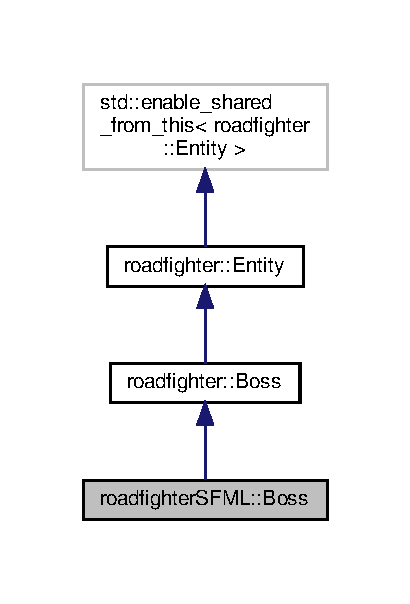
\includegraphics[width=197pt]{classroadfighterSFML_1_1Boss__inherit__graph}
\end{center}
\end{figure}


Collaboration diagram for roadfighter\+S\+F\+ML\+:\+:Boss\+:\nopagebreak
\begin{figure}[H]
\begin{center}
\leavevmode
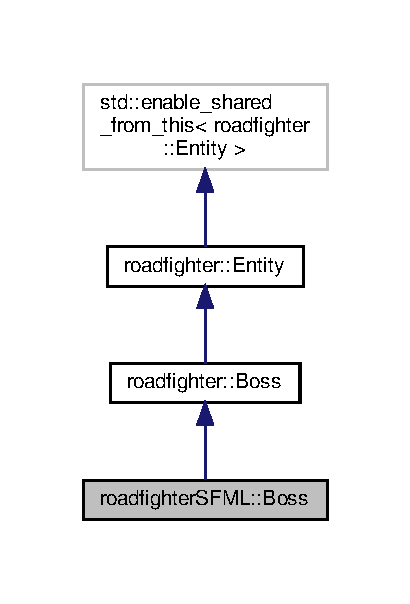
\includegraphics[width=197pt]{classroadfighterSFML_1_1Boss__coll__graph}
\end{center}
\end{figure}
\subsection*{Public Member Functions}
\begin{DoxyCompactItemize}
\item 
void \hyperlink{classroadfighterSFML_1_1Boss_a73041bc4cc4446fcf4605abe1052aa03}{draw} () override
\item 
\hyperlink{classroadfighterSFML_1_1Boss_ab56271ba9dfb9c945ee22cf7e5237d3d}{Boss} (const std\+::shared\+\_\+ptr$<$ sf\+::\+Render\+Window $>$ window, std\+::shared\+\_\+ptr$<$ \hyperlink{classConfigData}{Config\+Data} $>$ config)
\end{DoxyCompactItemize}
\subsection*{Additional Inherited Members}


\subsection{Detailed Description}
Graphic side of the boss 

\subsection{Constructor \& Destructor Documentation}
\mbox{\Hypertarget{classroadfighterSFML_1_1Boss_ab56271ba9dfb9c945ee22cf7e5237d3d}\label{classroadfighterSFML_1_1Boss_ab56271ba9dfb9c945ee22cf7e5237d3d}} 
\index{roadfighter\+S\+F\+M\+L\+::\+Boss@{roadfighter\+S\+F\+M\+L\+::\+Boss}!Boss@{Boss}}
\index{Boss@{Boss}!roadfighter\+S\+F\+M\+L\+::\+Boss@{roadfighter\+S\+F\+M\+L\+::\+Boss}}
\subsubsection{\texorpdfstring{Boss()}{Boss()}}
{\footnotesize\ttfamily roadfighter\+S\+F\+M\+L\+::\+Boss\+::\+Boss (\begin{DoxyParamCaption}\item[{const std\+::shared\+\_\+ptr$<$ sf\+::\+Render\+Window $>$}]{window,  }\item[{std\+::shared\+\_\+ptr$<$ \hyperlink{classConfigData}{Config\+Data} $>$}]{config }\end{DoxyParamCaption})}

Constructor with sfml window and configuration data 
\begin{DoxyParams}{Parameters}
{\em window} & \\
\hline
{\em config} & \\
\hline
\end{DoxyParams}


\subsection{Member Function Documentation}
\mbox{\Hypertarget{classroadfighterSFML_1_1Boss_a73041bc4cc4446fcf4605abe1052aa03}\label{classroadfighterSFML_1_1Boss_a73041bc4cc4446fcf4605abe1052aa03}} 
\index{roadfighter\+S\+F\+M\+L\+::\+Boss@{roadfighter\+S\+F\+M\+L\+::\+Boss}!draw@{draw}}
\index{draw@{draw}!roadfighter\+S\+F\+M\+L\+::\+Boss@{roadfighter\+S\+F\+M\+L\+::\+Boss}}
\subsubsection{\texorpdfstring{draw()}{draw()}}
{\footnotesize\ttfamily void roadfighter\+S\+F\+M\+L\+::\+Boss\+::draw (\begin{DoxyParamCaption}{ }\end{DoxyParamCaption})\hspace{0.3cm}{\ttfamily [override]}, {\ttfamily [virtual]}}

Draws the object 

Implements \hyperlink{classroadfighter_1_1Entity_ac516f8005f969ad5a86c252e5a3640ee}{roadfighter\+::\+Entity}.



The documentation for this class was generated from the following files\+:\begin{DoxyCompactItemize}
\item 
roadfighter\+S\+F\+M\+L/Boss.\+h\item 
roadfighter\+S\+F\+M\+L/Boss.\+cpp\end{DoxyCompactItemize}

\hypertarget{classroadfighter_1_1Bullet}{}\section{roadfighter\+:\+:Bullet Class Reference}
\label{classroadfighter_1_1Bullet}\index{roadfighter\+::\+Bullet@{roadfighter\+::\+Bullet}}


{\ttfamily \#include $<$Bullet.\+h$>$}



Inheritance diagram for roadfighter\+:\+:Bullet\+:\nopagebreak
\begin{figure}[H]
\begin{center}
\leavevmode
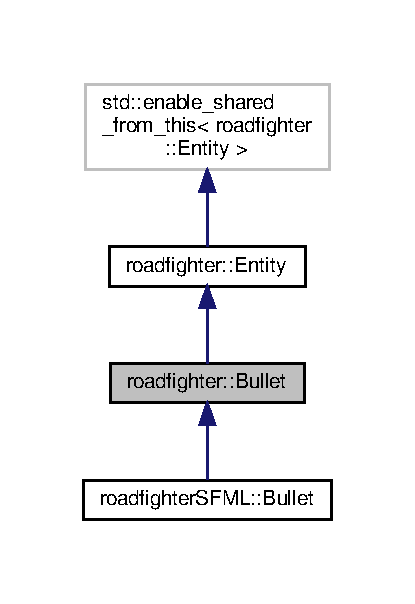
\includegraphics[width=199pt]{classroadfighter_1_1Bullet__inherit__graph}
\end{center}
\end{figure}


Collaboration diagram for roadfighter\+:\+:Bullet\+:\nopagebreak
\begin{figure}[H]
\begin{center}
\leavevmode
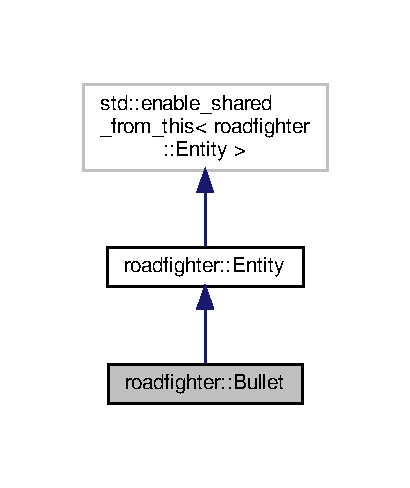
\includegraphics[width=197pt]{classroadfighter_1_1Bullet__coll__graph}
\end{center}
\end{figure}
\subsection*{Public Member Functions}
\begin{DoxyCompactItemize}
\item 
\hyperlink{classroadfighter_1_1Bullet_abcbb5d8fd968f182994fdbca0aab9f6d}{Bullet} (std\+::shared\+\_\+ptr$<$ \hyperlink{classConfigData}{Config\+Data} $>$ config)
\item 
void \hyperlink{classroadfighter_1_1Bullet_a9027c832dce3cd2839192255e0dbf301}{update} (int \hyperlink{classroadfighter_1_1Bullet_a88e3752878d08ceeaaaf307158f20d41}{speed}, std\+::shared\+\_\+ptr$<$ \hyperlink{classroadfighter_1_1Entity}{roadfighter\+::\+Entity} $>$ Player) override
\item 
void \hyperlink{classroadfighter_1_1Bullet_aab45c1cb9088b11c17e7a238543d8006}{update} () override
\item 
int \hyperlink{classroadfighter_1_1Bullet_ad05d66d01f1f839e1f38c6f12a0b091b}{get\+Speed} () override
\item 
int \hyperlink{classroadfighter_1_1Bullet_a011f2271222e0fa9bcf25193c2b94932}{Delete} () override
\item 
void \hyperlink{classroadfighter_1_1Bullet_ac3be16d9ff7da992fc6c5bd641f6d8dc}{set\+Delete} (int del) override
\item 
std\+::shared\+\_\+ptr$<$ \hyperlink{structObjBox}{Obj\+Box} $>$ \hyperlink{classroadfighter_1_1Bullet_a3e410865547614ec0470eb6ad18cc2c4}{get\+Objbox} () override
\item 
bool \hyperlink{classroadfighter_1_1Bullet_a0c093704ce5b9c2f4237d6b5dd1cbd36}{Shoot} () override
\end{DoxyCompactItemize}
\subsection*{Protected Attributes}
\begin{DoxyCompactItemize}
\item 
int \hyperlink{classroadfighter_1_1Bullet_a88e3752878d08ceeaaaf307158f20d41}{speed}
\item 
std\+::pair$<$ double, double $>$ \hyperlink{classroadfighter_1_1Bullet_a55d144151e85951e815d396a45701c8e}{pos}
\item 
int \hyperlink{classroadfighter_1_1Bullet_a400c93d89107eed04fff90f22dd37247}{to\+Del} = 0
\end{DoxyCompactItemize}


\subsection{Detailed Description}
\hyperlink{classroadfighter_1_1Bullet}{Bullet} class that gets used when the player shoohts 

\subsection{Constructor \& Destructor Documentation}
\mbox{\Hypertarget{classroadfighter_1_1Bullet_abcbb5d8fd968f182994fdbca0aab9f6d}\label{classroadfighter_1_1Bullet_abcbb5d8fd968f182994fdbca0aab9f6d}} 
\index{roadfighter\+::\+Bullet@{roadfighter\+::\+Bullet}!Bullet@{Bullet}}
\index{Bullet@{Bullet}!roadfighter\+::\+Bullet@{roadfighter\+::\+Bullet}}
\subsubsection{\texorpdfstring{Bullet()}{Bullet()}}
{\footnotesize\ttfamily roadfighter\+::\+Bullet\+::\+Bullet (\begin{DoxyParamCaption}\item[{std\+::shared\+\_\+ptr$<$ \hyperlink{classConfigData}{Config\+Data} $>$}]{config }\end{DoxyParamCaption})}

Constructor with configuration data 
\begin{DoxyParams}{Parameters}
{\em config} & \\
\hline
\end{DoxyParams}


\subsection{Member Function Documentation}
\mbox{\Hypertarget{classroadfighter_1_1Bullet_a011f2271222e0fa9bcf25193c2b94932}\label{classroadfighter_1_1Bullet_a011f2271222e0fa9bcf25193c2b94932}} 
\index{roadfighter\+::\+Bullet@{roadfighter\+::\+Bullet}!Delete@{Delete}}
\index{Delete@{Delete}!roadfighter\+::\+Bullet@{roadfighter\+::\+Bullet}}
\subsubsection{\texorpdfstring{Delete()}{Delete()}}
{\footnotesize\ttfamily int roadfighter\+::\+Bullet\+::\+Delete (\begin{DoxyParamCaption}{ }\end{DoxyParamCaption})\hspace{0.3cm}{\ttfamily [override]}, {\ttfamily [virtual]}}

Returns a certain value to determine the delete status 0 = nothing, 1 = delete, 2 = respawn \begin{DoxyReturn}{Returns}

\end{DoxyReturn}


Implements \hyperlink{classroadfighter_1_1Entity_a08190b0b8e6a3fcdb42273d6096152ac}{roadfighter\+::\+Entity}.

\mbox{\Hypertarget{classroadfighter_1_1Bullet_a3e410865547614ec0470eb6ad18cc2c4}\label{classroadfighter_1_1Bullet_a3e410865547614ec0470eb6ad18cc2c4}} 
\index{roadfighter\+::\+Bullet@{roadfighter\+::\+Bullet}!get\+Objbox@{get\+Objbox}}
\index{get\+Objbox@{get\+Objbox}!roadfighter\+::\+Bullet@{roadfighter\+::\+Bullet}}
\subsubsection{\texorpdfstring{get\+Objbox()}{getObjbox()}}
{\footnotesize\ttfamily std\+::shared\+\_\+ptr$<$ \hyperlink{structObjBox}{Obj\+Box} $>$ roadfighter\+::\+Bullet\+::get\+Objbox (\begin{DoxyParamCaption}{ }\end{DoxyParamCaption})\hspace{0.3cm}{\ttfamily [override]}, {\ttfamily [virtual]}}

Return the object box of an object \begin{DoxyReturn}{Returns}

\end{DoxyReturn}


Implements \hyperlink{classroadfighter_1_1Entity_af14340d04a725175a6d221f23c35fa0c}{roadfighter\+::\+Entity}.

\mbox{\Hypertarget{classroadfighter_1_1Bullet_ad05d66d01f1f839e1f38c6f12a0b091b}\label{classroadfighter_1_1Bullet_ad05d66d01f1f839e1f38c6f12a0b091b}} 
\index{roadfighter\+::\+Bullet@{roadfighter\+::\+Bullet}!get\+Speed@{get\+Speed}}
\index{get\+Speed@{get\+Speed}!roadfighter\+::\+Bullet@{roadfighter\+::\+Bullet}}
\subsubsection{\texorpdfstring{get\+Speed()}{getSpeed()}}
{\footnotesize\ttfamily int roadfighter\+::\+Bullet\+::get\+Speed (\begin{DoxyParamCaption}{ }\end{DoxyParamCaption})\hspace{0.3cm}{\ttfamily [override]}, {\ttfamily [virtual]}}

Returns the speed of the object \begin{DoxyReturn}{Returns}
speed 
\end{DoxyReturn}


Implements \hyperlink{classroadfighter_1_1Entity_ad3760184d764a61922e1db7d98501ee4}{roadfighter\+::\+Entity}.

\mbox{\Hypertarget{classroadfighter_1_1Bullet_ac3be16d9ff7da992fc6c5bd641f6d8dc}\label{classroadfighter_1_1Bullet_ac3be16d9ff7da992fc6c5bd641f6d8dc}} 
\index{roadfighter\+::\+Bullet@{roadfighter\+::\+Bullet}!set\+Delete@{set\+Delete}}
\index{set\+Delete@{set\+Delete}!roadfighter\+::\+Bullet@{roadfighter\+::\+Bullet}}
\subsubsection{\texorpdfstring{set\+Delete()}{setDelete()}}
{\footnotesize\ttfamily void roadfighter\+::\+Bullet\+::set\+Delete (\begin{DoxyParamCaption}\item[{int}]{del }\end{DoxyParamCaption})\hspace{0.3cm}{\ttfamily [override]}, {\ttfamily [virtual]}}

Set if an object must be deleted 
\begin{DoxyParams}{Parameters}
{\em del} & \\
\hline
\end{DoxyParams}


Implements \hyperlink{classroadfighter_1_1Entity_a07e973f0fa941a69e749629716877692}{roadfighter\+::\+Entity}.

\mbox{\Hypertarget{classroadfighter_1_1Bullet_a0c093704ce5b9c2f4237d6b5dd1cbd36}\label{classroadfighter_1_1Bullet_a0c093704ce5b9c2f4237d6b5dd1cbd36}} 
\index{roadfighter\+::\+Bullet@{roadfighter\+::\+Bullet}!Shoot@{Shoot}}
\index{Shoot@{Shoot}!roadfighter\+::\+Bullet@{roadfighter\+::\+Bullet}}
\subsubsection{\texorpdfstring{Shoot()}{Shoot()}}
{\footnotesize\ttfamily bool roadfighter\+::\+Bullet\+::\+Shoot (\begin{DoxyParamCaption}{ }\end{DoxyParamCaption})\hspace{0.3cm}{\ttfamily [override]}, {\ttfamily [virtual]}}

Return if an object must shoot; \begin{DoxyReturn}{Returns}

\end{DoxyReturn}


Implements \hyperlink{classroadfighter_1_1Entity_ad0ecaa0539db252e591da83814251509}{roadfighter\+::\+Entity}.

\mbox{\Hypertarget{classroadfighter_1_1Bullet_a9027c832dce3cd2839192255e0dbf301}\label{classroadfighter_1_1Bullet_a9027c832dce3cd2839192255e0dbf301}} 
\index{roadfighter\+::\+Bullet@{roadfighter\+::\+Bullet}!update@{update}}
\index{update@{update}!roadfighter\+::\+Bullet@{roadfighter\+::\+Bullet}}
\subsubsection{\texorpdfstring{update()}{update()}\hspace{0.1cm}{\footnotesize\ttfamily [1/2]}}
{\footnotesize\ttfamily void roadfighter\+::\+Bullet\+::update (\begin{DoxyParamCaption}\item[{int}]{speed,  }\item[{std\+::shared\+\_\+ptr$<$ \hyperlink{classroadfighter_1_1Entity}{roadfighter\+::\+Entity} $>$}]{Player }\end{DoxyParamCaption})\hspace{0.3cm}{\ttfamily [override]}, {\ttfamily [virtual]}}

Updates the object with extra parameters 
\begin{DoxyParams}{Parameters}
{\em speed} & \\
\hline
{\em Player} & \\
\hline
\end{DoxyParams}


Implements \hyperlink{classroadfighter_1_1Entity_a611ba56595dd2137d308876ba820cc09}{roadfighter\+::\+Entity}.

\mbox{\Hypertarget{classroadfighter_1_1Bullet_aab45c1cb9088b11c17e7a238543d8006}\label{classroadfighter_1_1Bullet_aab45c1cb9088b11c17e7a238543d8006}} 
\index{roadfighter\+::\+Bullet@{roadfighter\+::\+Bullet}!update@{update}}
\index{update@{update}!roadfighter\+::\+Bullet@{roadfighter\+::\+Bullet}}
\subsubsection{\texorpdfstring{update()}{update()}\hspace{0.1cm}{\footnotesize\ttfamily [2/2]}}
{\footnotesize\ttfamily void roadfighter\+::\+Bullet\+::update (\begin{DoxyParamCaption}{ }\end{DoxyParamCaption})\hspace{0.3cm}{\ttfamily [override]}, {\ttfamily [virtual]}}

Update the object 

Implements \hyperlink{classroadfighter_1_1Entity_a19cd353f12a3e8432acd6d5609137561}{roadfighter\+::\+Entity}.



\subsection{Member Data Documentation}
\mbox{\Hypertarget{classroadfighter_1_1Bullet_a55d144151e85951e815d396a45701c8e}\label{classroadfighter_1_1Bullet_a55d144151e85951e815d396a45701c8e}} 
\index{roadfighter\+::\+Bullet@{roadfighter\+::\+Bullet}!pos@{pos}}
\index{pos@{pos}!roadfighter\+::\+Bullet@{roadfighter\+::\+Bullet}}
\subsubsection{\texorpdfstring{pos}{pos}}
{\footnotesize\ttfamily std\+::pair$<$double, double$>$ roadfighter\+::\+Bullet\+::pos\hspace{0.3cm}{\ttfamily [protected]}}

Pair of the doubles that contains the x and y position of the center of the object \mbox{\Hypertarget{classroadfighter_1_1Bullet_a88e3752878d08ceeaaaf307158f20d41}\label{classroadfighter_1_1Bullet_a88e3752878d08ceeaaaf307158f20d41}} 
\index{roadfighter\+::\+Bullet@{roadfighter\+::\+Bullet}!speed@{speed}}
\index{speed@{speed}!roadfighter\+::\+Bullet@{roadfighter\+::\+Bullet}}
\subsubsection{\texorpdfstring{speed}{speed}}
{\footnotesize\ttfamily int roadfighter\+::\+Bullet\+::speed\hspace{0.3cm}{\ttfamily [protected]}}

Speed of the object \mbox{\Hypertarget{classroadfighter_1_1Bullet_a400c93d89107eed04fff90f22dd37247}\label{classroadfighter_1_1Bullet_a400c93d89107eed04fff90f22dd37247}} 
\index{roadfighter\+::\+Bullet@{roadfighter\+::\+Bullet}!to\+Del@{to\+Del}}
\index{to\+Del@{to\+Del}!roadfighter\+::\+Bullet@{roadfighter\+::\+Bullet}}
\subsubsection{\texorpdfstring{to\+Del}{toDel}}
{\footnotesize\ttfamily int roadfighter\+::\+Bullet\+::to\+Del = 0\hspace{0.3cm}{\ttfamily [protected]}}

Object deletion status ( 0 = nothing, 1 = delete, 2 = respawn ) 

The documentation for this class was generated from the following files\+:\begin{DoxyCompactItemize}
\item 
roadfighter/Bullet.\+h\item 
roadfighter/Bullet.\+cpp\end{DoxyCompactItemize}

\hypertarget{classroadfighterSFML_1_1Bullet}{}\section{roadfighter\+S\+F\+ML\+:\+:Bullet Class Reference}
\label{classroadfighterSFML_1_1Bullet}\index{roadfighter\+S\+F\+M\+L\+::\+Bullet@{roadfighter\+S\+F\+M\+L\+::\+Bullet}}


{\ttfamily \#include $<$Bullet.\+h$>$}



Inheritance diagram for roadfighter\+S\+F\+ML\+:\+:Bullet\+:\nopagebreak
\begin{figure}[H]
\begin{center}
\leavevmode
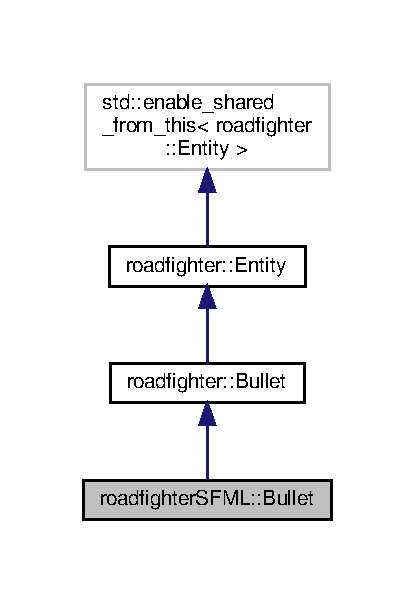
\includegraphics[width=199pt]{classroadfighterSFML_1_1Bullet__inherit__graph}
\end{center}
\end{figure}


Collaboration diagram for roadfighter\+S\+F\+ML\+:\+:Bullet\+:\nopagebreak
\begin{figure}[H]
\begin{center}
\leavevmode
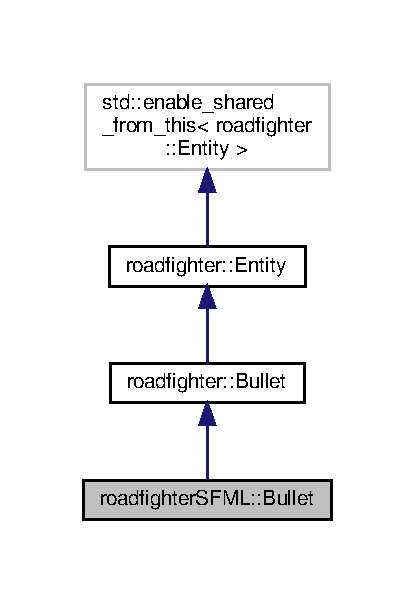
\includegraphics[width=199pt]{classroadfighterSFML_1_1Bullet__coll__graph}
\end{center}
\end{figure}
\subsection*{Public Member Functions}
\begin{DoxyCompactItemize}
\item 
void \hyperlink{classroadfighterSFML_1_1Bullet_a37d6977eace695d237c8859a0bcd413c}{draw} () override
\item 
\hyperlink{classroadfighterSFML_1_1Bullet_a396d4a5f8143e8c50d41d1ee0ae4c4fb}{Bullet} (const std\+::shared\+\_\+ptr$<$ sf\+::\+Render\+Window $>$ window, double first, double second, std\+::shared\+\_\+ptr$<$ \hyperlink{classConfigData}{Config\+Data} $>$ config)
\end{DoxyCompactItemize}
\subsection*{Additional Inherited Members}


\subsection{Detailed Description}
Graphic side of the bullet class 

\subsection{Constructor \& Destructor Documentation}
\mbox{\Hypertarget{classroadfighterSFML_1_1Bullet_a396d4a5f8143e8c50d41d1ee0ae4c4fb}\label{classroadfighterSFML_1_1Bullet_a396d4a5f8143e8c50d41d1ee0ae4c4fb}} 
\index{roadfighter\+S\+F\+M\+L\+::\+Bullet@{roadfighter\+S\+F\+M\+L\+::\+Bullet}!Bullet@{Bullet}}
\index{Bullet@{Bullet}!roadfighter\+S\+F\+M\+L\+::\+Bullet@{roadfighter\+S\+F\+M\+L\+::\+Bullet}}
\subsubsection{\texorpdfstring{Bullet()}{Bullet()}}
{\footnotesize\ttfamily roadfighter\+S\+F\+M\+L\+::\+Bullet\+::\+Bullet (\begin{DoxyParamCaption}\item[{const std\+::shared\+\_\+ptr$<$ sf\+::\+Render\+Window $>$}]{window,  }\item[{double}]{first,  }\item[{double}]{second,  }\item[{std\+::shared\+\_\+ptr$<$ \hyperlink{classConfigData}{Config\+Data} $>$}]{config }\end{DoxyParamCaption})}

Constructor with a window and the position and configuration data 
\begin{DoxyParams}{Parameters}
{\em window} & \\
\hline
{\em first} & \\
\hline
{\em second} & \\
\hline
{\em config} & \\
\hline
\end{DoxyParams}


\subsection{Member Function Documentation}
\mbox{\Hypertarget{classroadfighterSFML_1_1Bullet_a37d6977eace695d237c8859a0bcd413c}\label{classroadfighterSFML_1_1Bullet_a37d6977eace695d237c8859a0bcd413c}} 
\index{roadfighter\+S\+F\+M\+L\+::\+Bullet@{roadfighter\+S\+F\+M\+L\+::\+Bullet}!draw@{draw}}
\index{draw@{draw}!roadfighter\+S\+F\+M\+L\+::\+Bullet@{roadfighter\+S\+F\+M\+L\+::\+Bullet}}
\subsubsection{\texorpdfstring{draw()}{draw()}}
{\footnotesize\ttfamily void roadfighter\+S\+F\+M\+L\+::\+Bullet\+::draw (\begin{DoxyParamCaption}{ }\end{DoxyParamCaption})\hspace{0.3cm}{\ttfamily [override]}, {\ttfamily [virtual]}}

Draws the bullet 

Implements \hyperlink{classroadfighter_1_1Entity_ac516f8005f969ad5a86c252e5a3640ee}{roadfighter\+::\+Entity}.



The documentation for this class was generated from the following files\+:\begin{DoxyCompactItemize}
\item 
roadfighter\+S\+F\+M\+L/Bullet.\+h\item 
roadfighter\+S\+F\+M\+L/Bullet.\+cpp\end{DoxyCompactItemize}

\hypertarget{classConfigData}{}\section{Config\+Data Class Reference}
\label{classConfigData}\index{Config\+Data@{Config\+Data}}


{\ttfamily \#include $<$Config\+Data.\+h$>$}

\subsection*{Public Member Functions}
\begin{DoxyCompactItemize}
\item 
\hyperlink{classConfigData_ab5aa8113ed01a5d906c11cc722a34bf1}{Config\+Data} (std\+::string filename)
\item 
const std\+::string \& \hyperlink{classConfigData_a2ebc3e9c59f5d799cc241c528a2a90b1}{get\+Font} () const
\item 
const std\+::string \& \hyperlink{classConfigData_a2e2c571c1dc23cc301a0dba85de97357}{get\+Level1} () const
\item 
const std\+::string \& \hyperlink{classConfigData_a073531011ba29efe96cb682801b778e7}{get\+Level2} () const
\item 
const std\+::string \& \hyperlink{classConfigData_a995d48538315ad108eed0cbd0eaaae69}{get\+Level3} () const
\item 
const std\+::string \& \hyperlink{classConfigData_a8b91e6a3dfe7cb880e9c5d43b6f0e00b}{get\+Highscore} () const
\item 
const std\+::string \& \hyperlink{classConfigData_a3c4ea1cdbbc1635fce4efec4b4aa1abd}{get\+Ai} () const
\item 
const std\+::string \& \hyperlink{classConfigData_a14b80899285714c7d72330fef05d643d}{get\+Background1} () const
\item 
const std\+::string \& \hyperlink{classConfigData_abaf686c98923cbd5b25d1135988499e7}{get\+Background2} () const
\item 
const std\+::string \& \hyperlink{classConfigData_a374fdf7f1d3275a86b08880133fa0e16}{get\+Background3} () const
\item 
const std\+::string \& \hyperlink{classConfigData_a73f750c44eee20c091b2a3984b42f5ec}{get\+Background1\+Fin} () const
\item 
const std\+::string \& \hyperlink{classConfigData_ab4a6bf95cb21298a472a17763d56c35d}{get\+Background2\+Fin} () const
\item 
const std\+::string \& \hyperlink{classConfigData_aedb142fd1f37b67f0c6136ce0d7f2399}{get\+Background3\+Fin} () const
\item 
const std\+::string \& \hyperlink{classConfigData_a241de31080d870efdde3046d7d9a96b8}{get\+Boss} () const
\item 
const std\+::string \& \hyperlink{classConfigData_a087b7790faec74ef110bd2d810338858}{get\+Bullet} () const
\item 
const std\+::string \& \hyperlink{classConfigData_a79e097cdf1cc394818bb399cc4662176}{get\+Moving\+Car} () const
\item 
const std\+::string \& \hyperlink{classConfigData_a5bc69646f744c91350126a83fe3a8199}{get\+Passing\+Car} () const
\item 
const std\+::string \& \hyperlink{classConfigData_a457424b879afddb0c95273e5ac16badd}{get\+Player} () const
\item 
const std\+::string \& \hyperlink{classConfigData_a9990a42f4759f46479488e1fb912f7b6}{get\+Rock} () const
\item 
int \hyperlink{classConfigData_a6ddf5ff9a004d3b236622e900a652922}{get\+Respawn\+Timer\+Ai} () const
\item 
int \hyperlink{classConfigData_ad9c86352ac8cabb3817eadf52dee0605}{get\+Max\+Speed\+Ai} () const
\item 
int \hyperlink{classConfigData_a8ac967cae90e657e68fbd0d1e163f0ec}{get\+Acceleration\+Ai} () const
\item 
int \hyperlink{classConfigData_ad815c66b9580b9a8bc4eda6ce2cb0e80}{get\+Distance} () const
\item 
int \hyperlink{classConfigData_a115ef1483345c4b89e9984f370dabbcc}{get\+Respawn\+Timer\+Player} () const
\item 
int \hyperlink{classConfigData_ab791ddf310f5dd0f0ed12752dcae18bc}{get\+Max\+Speed\+Player} () const
\item 
int \hyperlink{classConfigData_a7889ad0ddf98c026ef9996a8d09f7337}{get\+Acceleration\+Player} () const
\item 
int \hyperlink{classConfigData_ae74cc34be85fd4265e491c2717ab9638}{get\+Bossfight\+Speed} () const
\item 
int \hyperlink{classConfigData_a3081c0e98b204b3f05fb06c98f7d216e}{get\+Reload\+Speed} () const
\item 
int \hyperlink{classConfigData_acc83f639f36dd93dee1f4bf2cf3cb374}{get\+Max\+Speed\+Passing\+Car} () const
\item 
int \hyperlink{classConfigData_a0251ca808c712d27def8a6d164934a30}{get\+Bullet\+Speed} () const
\item 
int \hyperlink{classConfigData_a90fb727b6f5583b2388a1c0bd853bc1a}{get\+Lifes} () const
\item 
int \hyperlink{classConfigData_ae73ba005cb7df3b2e9c38cb216324b05}{get\+Attack\+Timer} () const
\item 
int \hyperlink{classConfigData_a732dfa16f1cc3a38c734e7cef107300a}{get\+Game\+Ending\+Timer} () const
\item 
int \hyperlink{classConfigData_a482dbfc0bae40a9b690bdcafc9de1e9a}{get\+Car\+Spawn\+Timer} () const
\item 
int \hyperlink{classConfigData_a7decc7f3a25937fd169f2908b27c3565}{get\+Rock\+Spawn\+Timer} () const
\item 
void \hyperlink{classConfigData_a43959934e2e3a927e142203e637e327a}{set\+Background1} (const std\+::string \&background1)
\item 
void \hyperlink{classConfigData_a8502ce728edf1a3d835c5fcafe6d4e30}{set\+Background2} (const std\+::string \&background2)
\item 
void \hyperlink{classConfigData_a339eecd0d675c97642969024a2ab4ff5}{set\+Background3} (const std\+::string \&background3)
\item 
void \hyperlink{classConfigData_a9f242df86492feeae19aed291af32bd3}{set\+Background1\+Fin} (const std\+::string \&background1\+Fin)
\item 
void \hyperlink{classConfigData_aba02fb9632f972bd7359e8deca226b26}{set\+Background2\+Fin} (const std\+::string \&background2\+Fin)
\item 
void \hyperlink{classConfigData_ad2b64a90240c5f3d3b84f398c339a6b7}{set\+Background3\+Fin} (const std\+::string \&background3\+Fin)
\end{DoxyCompactItemize}


\subsection{Detailed Description}
Holds all the data given by the configuration file 

\subsection{Constructor \& Destructor Documentation}
\mbox{\Hypertarget{classConfigData_ab5aa8113ed01a5d906c11cc722a34bf1}\label{classConfigData_ab5aa8113ed01a5d906c11cc722a34bf1}} 
\index{Config\+Data@{Config\+Data}!Config\+Data@{Config\+Data}}
\index{Config\+Data@{Config\+Data}!Config\+Data@{Config\+Data}}
\subsubsection{\texorpdfstring{Config\+Data()}{ConfigData()}}
{\footnotesize\ttfamily Config\+Data\+::\+Config\+Data (\begin{DoxyParamCaption}\item[{std\+::string}]{filename }\end{DoxyParamCaption})}

Constructor that parses the config file 
\begin{DoxyParams}{Parameters}
{\em filename} & \\
\hline
\end{DoxyParams}


\subsection{Member Function Documentation}
\mbox{\Hypertarget{classConfigData_a8ac967cae90e657e68fbd0d1e163f0ec}\label{classConfigData_a8ac967cae90e657e68fbd0d1e163f0ec}} 
\index{Config\+Data@{Config\+Data}!get\+Acceleration\+Ai@{get\+Acceleration\+Ai}}
\index{get\+Acceleration\+Ai@{get\+Acceleration\+Ai}!Config\+Data@{Config\+Data}}
\subsubsection{\texorpdfstring{get\+Acceleration\+Ai()}{getAccelerationAi()}}
{\footnotesize\ttfamily int Config\+Data\+::get\+Acceleration\+Ai (\begin{DoxyParamCaption}{ }\end{DoxyParamCaption}) const}

Getter for the acceleration of the AI \begin{DoxyReturn}{Returns}

\end{DoxyReturn}
\mbox{\Hypertarget{classConfigData_a7889ad0ddf98c026ef9996a8d09f7337}\label{classConfigData_a7889ad0ddf98c026ef9996a8d09f7337}} 
\index{Config\+Data@{Config\+Data}!get\+Acceleration\+Player@{get\+Acceleration\+Player}}
\index{get\+Acceleration\+Player@{get\+Acceleration\+Player}!Config\+Data@{Config\+Data}}
\subsubsection{\texorpdfstring{get\+Acceleration\+Player()}{getAccelerationPlayer()}}
{\footnotesize\ttfamily int Config\+Data\+::get\+Acceleration\+Player (\begin{DoxyParamCaption}{ }\end{DoxyParamCaption}) const}

Getter for the acceleration of the player \begin{DoxyReturn}{Returns}

\end{DoxyReturn}
\mbox{\Hypertarget{classConfigData_a3c4ea1cdbbc1635fce4efec4b4aa1abd}\label{classConfigData_a3c4ea1cdbbc1635fce4efec4b4aa1abd}} 
\index{Config\+Data@{Config\+Data}!get\+Ai@{get\+Ai}}
\index{get\+Ai@{get\+Ai}!Config\+Data@{Config\+Data}}
\subsubsection{\texorpdfstring{get\+Ai()}{getAi()}}
{\footnotesize\ttfamily const std\+::string \& Config\+Data\+::get\+Ai (\begin{DoxyParamCaption}{ }\end{DoxyParamCaption}) const}

Getter for the AI sprite \begin{DoxyReturn}{Returns}

\end{DoxyReturn}
\mbox{\Hypertarget{classConfigData_ae73ba005cb7df3b2e9c38cb216324b05}\label{classConfigData_ae73ba005cb7df3b2e9c38cb216324b05}} 
\index{Config\+Data@{Config\+Data}!get\+Attack\+Timer@{get\+Attack\+Timer}}
\index{get\+Attack\+Timer@{get\+Attack\+Timer}!Config\+Data@{Config\+Data}}
\subsubsection{\texorpdfstring{get\+Attack\+Timer()}{getAttackTimer()}}
{\footnotesize\ttfamily int Config\+Data\+::get\+Attack\+Timer (\begin{DoxyParamCaption}{ }\end{DoxyParamCaption}) const}

Getter for the attack timer of the boss (time between attacks) \begin{DoxyReturn}{Returns}

\end{DoxyReturn}
\mbox{\Hypertarget{classConfigData_a14b80899285714c7d72330fef05d643d}\label{classConfigData_a14b80899285714c7d72330fef05d643d}} 
\index{Config\+Data@{Config\+Data}!get\+Background1@{get\+Background1}}
\index{get\+Background1@{get\+Background1}!Config\+Data@{Config\+Data}}
\subsubsection{\texorpdfstring{get\+Background1()}{getBackground1()}}
{\footnotesize\ttfamily const std\+::string \& Config\+Data\+::get\+Background1 (\begin{DoxyParamCaption}{ }\end{DoxyParamCaption}) const}

Getter for the level 1 background sprite \begin{DoxyReturn}{Returns}

\end{DoxyReturn}
\mbox{\Hypertarget{classConfigData_a73f750c44eee20c091b2a3984b42f5ec}\label{classConfigData_a73f750c44eee20c091b2a3984b42f5ec}} 
\index{Config\+Data@{Config\+Data}!get\+Background1\+Fin@{get\+Background1\+Fin}}
\index{get\+Background1\+Fin@{get\+Background1\+Fin}!Config\+Data@{Config\+Data}}
\subsubsection{\texorpdfstring{get\+Background1\+Fin()}{getBackground1Fin()}}
{\footnotesize\ttfamily const std\+::string \& Config\+Data\+::get\+Background1\+Fin (\begin{DoxyParamCaption}{ }\end{DoxyParamCaption}) const}

Getter for the level 1 background finish sprite \begin{DoxyReturn}{Returns}

\end{DoxyReturn}
\mbox{\Hypertarget{classConfigData_abaf686c98923cbd5b25d1135988499e7}\label{classConfigData_abaf686c98923cbd5b25d1135988499e7}} 
\index{Config\+Data@{Config\+Data}!get\+Background2@{get\+Background2}}
\index{get\+Background2@{get\+Background2}!Config\+Data@{Config\+Data}}
\subsubsection{\texorpdfstring{get\+Background2()}{getBackground2()}}
{\footnotesize\ttfamily const std\+::string \& Config\+Data\+::get\+Background2 (\begin{DoxyParamCaption}{ }\end{DoxyParamCaption}) const}

Getter for the level 2 background sprite \begin{DoxyReturn}{Returns}

\end{DoxyReturn}
\mbox{\Hypertarget{classConfigData_ab4a6bf95cb21298a472a17763d56c35d}\label{classConfigData_ab4a6bf95cb21298a472a17763d56c35d}} 
\index{Config\+Data@{Config\+Data}!get\+Background2\+Fin@{get\+Background2\+Fin}}
\index{get\+Background2\+Fin@{get\+Background2\+Fin}!Config\+Data@{Config\+Data}}
\subsubsection{\texorpdfstring{get\+Background2\+Fin()}{getBackground2Fin()}}
{\footnotesize\ttfamily const std\+::string \& Config\+Data\+::get\+Background2\+Fin (\begin{DoxyParamCaption}{ }\end{DoxyParamCaption}) const}

Getter for the level 2 background finish sprite \begin{DoxyReturn}{Returns}

\end{DoxyReturn}
\mbox{\Hypertarget{classConfigData_a374fdf7f1d3275a86b08880133fa0e16}\label{classConfigData_a374fdf7f1d3275a86b08880133fa0e16}} 
\index{Config\+Data@{Config\+Data}!get\+Background3@{get\+Background3}}
\index{get\+Background3@{get\+Background3}!Config\+Data@{Config\+Data}}
\subsubsection{\texorpdfstring{get\+Background3()}{getBackground3()}}
{\footnotesize\ttfamily const std\+::string \& Config\+Data\+::get\+Background3 (\begin{DoxyParamCaption}{ }\end{DoxyParamCaption}) const}

Getter for the level 3 background sprite \begin{DoxyReturn}{Returns}

\end{DoxyReturn}
\mbox{\Hypertarget{classConfigData_aedb142fd1f37b67f0c6136ce0d7f2399}\label{classConfigData_aedb142fd1f37b67f0c6136ce0d7f2399}} 
\index{Config\+Data@{Config\+Data}!get\+Background3\+Fin@{get\+Background3\+Fin}}
\index{get\+Background3\+Fin@{get\+Background3\+Fin}!Config\+Data@{Config\+Data}}
\subsubsection{\texorpdfstring{get\+Background3\+Fin()}{getBackground3Fin()}}
{\footnotesize\ttfamily const std\+::string \& Config\+Data\+::get\+Background3\+Fin (\begin{DoxyParamCaption}{ }\end{DoxyParamCaption}) const}

Getter for the level 3 background finish sprite \begin{DoxyReturn}{Returns}

\end{DoxyReturn}
\mbox{\Hypertarget{classConfigData_a241de31080d870efdde3046d7d9a96b8}\label{classConfigData_a241de31080d870efdde3046d7d9a96b8}} 
\index{Config\+Data@{Config\+Data}!get\+Boss@{get\+Boss}}
\index{get\+Boss@{get\+Boss}!Config\+Data@{Config\+Data}}
\subsubsection{\texorpdfstring{get\+Boss()}{getBoss()}}
{\footnotesize\ttfamily const std\+::string \& Config\+Data\+::get\+Boss (\begin{DoxyParamCaption}{ }\end{DoxyParamCaption}) const}

Getter for the boss sprite \begin{DoxyReturn}{Returns}

\end{DoxyReturn}
\mbox{\Hypertarget{classConfigData_ae74cc34be85fd4265e491c2717ab9638}\label{classConfigData_ae74cc34be85fd4265e491c2717ab9638}} 
\index{Config\+Data@{Config\+Data}!get\+Bossfight\+Speed@{get\+Bossfight\+Speed}}
\index{get\+Bossfight\+Speed@{get\+Bossfight\+Speed}!Config\+Data@{Config\+Data}}
\subsubsection{\texorpdfstring{get\+Bossfight\+Speed()}{getBossfightSpeed()}}
{\footnotesize\ttfamily int Config\+Data\+::get\+Bossfight\+Speed (\begin{DoxyParamCaption}{ }\end{DoxyParamCaption}) const}

Getter for the static speed during the bossfight \begin{DoxyReturn}{Returns}

\end{DoxyReturn}
\mbox{\Hypertarget{classConfigData_a087b7790faec74ef110bd2d810338858}\label{classConfigData_a087b7790faec74ef110bd2d810338858}} 
\index{Config\+Data@{Config\+Data}!get\+Bullet@{get\+Bullet}}
\index{get\+Bullet@{get\+Bullet}!Config\+Data@{Config\+Data}}
\subsubsection{\texorpdfstring{get\+Bullet()}{getBullet()}}
{\footnotesize\ttfamily const std\+::string \& Config\+Data\+::get\+Bullet (\begin{DoxyParamCaption}{ }\end{DoxyParamCaption}) const}

Getter for the bullet sprite \begin{DoxyReturn}{Returns}

\end{DoxyReturn}
\mbox{\Hypertarget{classConfigData_a0251ca808c712d27def8a6d164934a30}\label{classConfigData_a0251ca808c712d27def8a6d164934a30}} 
\index{Config\+Data@{Config\+Data}!get\+Bullet\+Speed@{get\+Bullet\+Speed}}
\index{get\+Bullet\+Speed@{get\+Bullet\+Speed}!Config\+Data@{Config\+Data}}
\subsubsection{\texorpdfstring{get\+Bullet\+Speed()}{getBulletSpeed()}}
{\footnotesize\ttfamily int Config\+Data\+::get\+Bullet\+Speed (\begin{DoxyParamCaption}{ }\end{DoxyParamCaption}) const}

Getter for the bullet speed \begin{DoxyReturn}{Returns}

\end{DoxyReturn}
\mbox{\Hypertarget{classConfigData_a482dbfc0bae40a9b690bdcafc9de1e9a}\label{classConfigData_a482dbfc0bae40a9b690bdcafc9de1e9a}} 
\index{Config\+Data@{Config\+Data}!get\+Car\+Spawn\+Timer@{get\+Car\+Spawn\+Timer}}
\index{get\+Car\+Spawn\+Timer@{get\+Car\+Spawn\+Timer}!Config\+Data@{Config\+Data}}
\subsubsection{\texorpdfstring{get\+Car\+Spawn\+Timer()}{getCarSpawnTimer()}}
{\footnotesize\ttfamily int Config\+Data\+::get\+Car\+Spawn\+Timer (\begin{DoxyParamCaption}{ }\end{DoxyParamCaption}) const}

Getter for the timer to spawn cars (time between cars that spawn) \begin{DoxyReturn}{Returns}

\end{DoxyReturn}
\mbox{\Hypertarget{classConfigData_ad815c66b9580b9a8bc4eda6ce2cb0e80}\label{classConfigData_ad815c66b9580b9a8bc4eda6ce2cb0e80}} 
\index{Config\+Data@{Config\+Data}!get\+Distance@{get\+Distance}}
\index{get\+Distance@{get\+Distance}!Config\+Data@{Config\+Data}}
\subsubsection{\texorpdfstring{get\+Distance()}{getDistance()}}
{\footnotesize\ttfamily int Config\+Data\+::get\+Distance (\begin{DoxyParamCaption}{ }\end{DoxyParamCaption}) const}

Getter for the travel distance \begin{DoxyReturn}{Returns}

\end{DoxyReturn}
\mbox{\Hypertarget{classConfigData_a2ebc3e9c59f5d799cc241c528a2a90b1}\label{classConfigData_a2ebc3e9c59f5d799cc241c528a2a90b1}} 
\index{Config\+Data@{Config\+Data}!get\+Font@{get\+Font}}
\index{get\+Font@{get\+Font}!Config\+Data@{Config\+Data}}
\subsubsection{\texorpdfstring{get\+Font()}{getFont()}}
{\footnotesize\ttfamily const std\+::string \& Config\+Data\+::get\+Font (\begin{DoxyParamCaption}{ }\end{DoxyParamCaption}) const}

Getter for the font \begin{DoxyReturn}{Returns}

\end{DoxyReturn}
\mbox{\Hypertarget{classConfigData_a732dfa16f1cc3a38c734e7cef107300a}\label{classConfigData_a732dfa16f1cc3a38c734e7cef107300a}} 
\index{Config\+Data@{Config\+Data}!get\+Game\+Ending\+Timer@{get\+Game\+Ending\+Timer}}
\index{get\+Game\+Ending\+Timer@{get\+Game\+Ending\+Timer}!Config\+Data@{Config\+Data}}
\subsubsection{\texorpdfstring{get\+Game\+Ending\+Timer()}{getGameEndingTimer()}}
{\footnotesize\ttfamily int Config\+Data\+::get\+Game\+Ending\+Timer (\begin{DoxyParamCaption}{ }\end{DoxyParamCaption}) const}

Getter for the ending timer of the game \begin{DoxyReturn}{Returns}

\end{DoxyReturn}
\mbox{\Hypertarget{classConfigData_a8b91e6a3dfe7cb880e9c5d43b6f0e00b}\label{classConfigData_a8b91e6a3dfe7cb880e9c5d43b6f0e00b}} 
\index{Config\+Data@{Config\+Data}!get\+Highscore@{get\+Highscore}}
\index{get\+Highscore@{get\+Highscore}!Config\+Data@{Config\+Data}}
\subsubsection{\texorpdfstring{get\+Highscore()}{getHighscore()}}
{\footnotesize\ttfamily const std\+::string \& Config\+Data\+::get\+Highscore (\begin{DoxyParamCaption}{ }\end{DoxyParamCaption}) const}

Getter for the high-\/score file \begin{DoxyReturn}{Returns}

\end{DoxyReturn}
\mbox{\Hypertarget{classConfigData_a2e2c571c1dc23cc301a0dba85de97357}\label{classConfigData_a2e2c571c1dc23cc301a0dba85de97357}} 
\index{Config\+Data@{Config\+Data}!get\+Level1@{get\+Level1}}
\index{get\+Level1@{get\+Level1}!Config\+Data@{Config\+Data}}
\subsubsection{\texorpdfstring{get\+Level1()}{getLevel1()}}
{\footnotesize\ttfamily const std\+::string \& Config\+Data\+::get\+Level1 (\begin{DoxyParamCaption}{ }\end{DoxyParamCaption}) const}

Getter for the first level file \begin{DoxyReturn}{Returns}

\end{DoxyReturn}
\mbox{\Hypertarget{classConfigData_a073531011ba29efe96cb682801b778e7}\label{classConfigData_a073531011ba29efe96cb682801b778e7}} 
\index{Config\+Data@{Config\+Data}!get\+Level2@{get\+Level2}}
\index{get\+Level2@{get\+Level2}!Config\+Data@{Config\+Data}}
\subsubsection{\texorpdfstring{get\+Level2()}{getLevel2()}}
{\footnotesize\ttfamily const std\+::string \& Config\+Data\+::get\+Level2 (\begin{DoxyParamCaption}{ }\end{DoxyParamCaption}) const}

Getter for the second level file \begin{DoxyReturn}{Returns}

\end{DoxyReturn}
\mbox{\Hypertarget{classConfigData_a995d48538315ad108eed0cbd0eaaae69}\label{classConfigData_a995d48538315ad108eed0cbd0eaaae69}} 
\index{Config\+Data@{Config\+Data}!get\+Level3@{get\+Level3}}
\index{get\+Level3@{get\+Level3}!Config\+Data@{Config\+Data}}
\subsubsection{\texorpdfstring{get\+Level3()}{getLevel3()}}
{\footnotesize\ttfamily const std\+::string \& Config\+Data\+::get\+Level3 (\begin{DoxyParamCaption}{ }\end{DoxyParamCaption}) const}

Getter for the third level file \begin{DoxyReturn}{Returns}

\end{DoxyReturn}
\mbox{\Hypertarget{classConfigData_a90fb727b6f5583b2388a1c0bd853bc1a}\label{classConfigData_a90fb727b6f5583b2388a1c0bd853bc1a}} 
\index{Config\+Data@{Config\+Data}!get\+Lifes@{get\+Lifes}}
\index{get\+Lifes@{get\+Lifes}!Config\+Data@{Config\+Data}}
\subsubsection{\texorpdfstring{get\+Lifes()}{getLifes()}}
{\footnotesize\ttfamily int Config\+Data\+::get\+Lifes (\begin{DoxyParamCaption}{ }\end{DoxyParamCaption}) const}

Getter for the lifes of the boss \begin{DoxyReturn}{Returns}

\end{DoxyReturn}
\mbox{\Hypertarget{classConfigData_ad9c86352ac8cabb3817eadf52dee0605}\label{classConfigData_ad9c86352ac8cabb3817eadf52dee0605}} 
\index{Config\+Data@{Config\+Data}!get\+Max\+Speed\+Ai@{get\+Max\+Speed\+Ai}}
\index{get\+Max\+Speed\+Ai@{get\+Max\+Speed\+Ai}!Config\+Data@{Config\+Data}}
\subsubsection{\texorpdfstring{get\+Max\+Speed\+Ai()}{getMaxSpeedAi()}}
{\footnotesize\ttfamily int Config\+Data\+::get\+Max\+Speed\+Ai (\begin{DoxyParamCaption}{ }\end{DoxyParamCaption}) const}

Getter for the max speed of the AI \begin{DoxyReturn}{Returns}

\end{DoxyReturn}
\mbox{\Hypertarget{classConfigData_acc83f639f36dd93dee1f4bf2cf3cb374}\label{classConfigData_acc83f639f36dd93dee1f4bf2cf3cb374}} 
\index{Config\+Data@{Config\+Data}!get\+Max\+Speed\+Passing\+Car@{get\+Max\+Speed\+Passing\+Car}}
\index{get\+Max\+Speed\+Passing\+Car@{get\+Max\+Speed\+Passing\+Car}!Config\+Data@{Config\+Data}}
\subsubsection{\texorpdfstring{get\+Max\+Speed\+Passing\+Car()}{getMaxSpeedPassingCar()}}
{\footnotesize\ttfamily int Config\+Data\+::get\+Max\+Speed\+Passing\+Car (\begin{DoxyParamCaption}{ }\end{DoxyParamCaption}) const}

Getter for the max speed of the passingcar \begin{DoxyReturn}{Returns}

\end{DoxyReturn}
\mbox{\Hypertarget{classConfigData_ab791ddf310f5dd0f0ed12752dcae18bc}\label{classConfigData_ab791ddf310f5dd0f0ed12752dcae18bc}} 
\index{Config\+Data@{Config\+Data}!get\+Max\+Speed\+Player@{get\+Max\+Speed\+Player}}
\index{get\+Max\+Speed\+Player@{get\+Max\+Speed\+Player}!Config\+Data@{Config\+Data}}
\subsubsection{\texorpdfstring{get\+Max\+Speed\+Player()}{getMaxSpeedPlayer()}}
{\footnotesize\ttfamily int Config\+Data\+::get\+Max\+Speed\+Player (\begin{DoxyParamCaption}{ }\end{DoxyParamCaption}) const}

Getter for the max speed of the player \begin{DoxyReturn}{Returns}

\end{DoxyReturn}
\mbox{\Hypertarget{classConfigData_a79e097cdf1cc394818bb399cc4662176}\label{classConfigData_a79e097cdf1cc394818bb399cc4662176}} 
\index{Config\+Data@{Config\+Data}!get\+Moving\+Car@{get\+Moving\+Car}}
\index{get\+Moving\+Car@{get\+Moving\+Car}!Config\+Data@{Config\+Data}}
\subsubsection{\texorpdfstring{get\+Moving\+Car()}{getMovingCar()}}
{\footnotesize\ttfamily const std\+::string \& Config\+Data\+::get\+Moving\+Car (\begin{DoxyParamCaption}{ }\end{DoxyParamCaption}) const}

Getter for the movingcar sprite \begin{DoxyReturn}{Returns}

\end{DoxyReturn}
\mbox{\Hypertarget{classConfigData_a5bc69646f744c91350126a83fe3a8199}\label{classConfigData_a5bc69646f744c91350126a83fe3a8199}} 
\index{Config\+Data@{Config\+Data}!get\+Passing\+Car@{get\+Passing\+Car}}
\index{get\+Passing\+Car@{get\+Passing\+Car}!Config\+Data@{Config\+Data}}
\subsubsection{\texorpdfstring{get\+Passing\+Car()}{getPassingCar()}}
{\footnotesize\ttfamily const std\+::string \& Config\+Data\+::get\+Passing\+Car (\begin{DoxyParamCaption}{ }\end{DoxyParamCaption}) const}

Getter for passingcar sprite \begin{DoxyReturn}{Returns}

\end{DoxyReturn}
\mbox{\Hypertarget{classConfigData_a457424b879afddb0c95273e5ac16badd}\label{classConfigData_a457424b879afddb0c95273e5ac16badd}} 
\index{Config\+Data@{Config\+Data}!get\+Player@{get\+Player}}
\index{get\+Player@{get\+Player}!Config\+Data@{Config\+Data}}
\subsubsection{\texorpdfstring{get\+Player()}{getPlayer()}}
{\footnotesize\ttfamily const std\+::string \& Config\+Data\+::get\+Player (\begin{DoxyParamCaption}{ }\end{DoxyParamCaption}) const}

Getter for the player sprite \begin{DoxyReturn}{Returns}

\end{DoxyReturn}
\mbox{\Hypertarget{classConfigData_a3081c0e98b204b3f05fb06c98f7d216e}\label{classConfigData_a3081c0e98b204b3f05fb06c98f7d216e}} 
\index{Config\+Data@{Config\+Data}!get\+Reload\+Speed@{get\+Reload\+Speed}}
\index{get\+Reload\+Speed@{get\+Reload\+Speed}!Config\+Data@{Config\+Data}}
\subsubsection{\texorpdfstring{get\+Reload\+Speed()}{getReloadSpeed()}}
{\footnotesize\ttfamily int Config\+Data\+::get\+Reload\+Speed (\begin{DoxyParamCaption}{ }\end{DoxyParamCaption}) const}

Get the reload speed \begin{DoxyReturn}{Returns}

\end{DoxyReturn}
\mbox{\Hypertarget{classConfigData_a6ddf5ff9a004d3b236622e900a652922}\label{classConfigData_a6ddf5ff9a004d3b236622e900a652922}} 
\index{Config\+Data@{Config\+Data}!get\+Respawn\+Timer\+Ai@{get\+Respawn\+Timer\+Ai}}
\index{get\+Respawn\+Timer\+Ai@{get\+Respawn\+Timer\+Ai}!Config\+Data@{Config\+Data}}
\subsubsection{\texorpdfstring{get\+Respawn\+Timer\+Ai()}{getRespawnTimerAi()}}
{\footnotesize\ttfamily int Config\+Data\+::get\+Respawn\+Timer\+Ai (\begin{DoxyParamCaption}{ }\end{DoxyParamCaption}) const}

Getter for the respawntimer for the AI \begin{DoxyReturn}{Returns}

\end{DoxyReturn}
\mbox{\Hypertarget{classConfigData_a115ef1483345c4b89e9984f370dabbcc}\label{classConfigData_a115ef1483345c4b89e9984f370dabbcc}} 
\index{Config\+Data@{Config\+Data}!get\+Respawn\+Timer\+Player@{get\+Respawn\+Timer\+Player}}
\index{get\+Respawn\+Timer\+Player@{get\+Respawn\+Timer\+Player}!Config\+Data@{Config\+Data}}
\subsubsection{\texorpdfstring{get\+Respawn\+Timer\+Player()}{getRespawnTimerPlayer()}}
{\footnotesize\ttfamily int Config\+Data\+::get\+Respawn\+Timer\+Player (\begin{DoxyParamCaption}{ }\end{DoxyParamCaption}) const}

Getter for the respawn timer of the player \begin{DoxyReturn}{Returns}

\end{DoxyReturn}
\mbox{\Hypertarget{classConfigData_a9990a42f4759f46479488e1fb912f7b6}\label{classConfigData_a9990a42f4759f46479488e1fb912f7b6}} 
\index{Config\+Data@{Config\+Data}!get\+Rock@{get\+Rock}}
\index{get\+Rock@{get\+Rock}!Config\+Data@{Config\+Data}}
\subsubsection{\texorpdfstring{get\+Rock()}{getRock()}}
{\footnotesize\ttfamily const std\+::string \& Config\+Data\+::get\+Rock (\begin{DoxyParamCaption}{ }\end{DoxyParamCaption}) const}

Getter for the rock sprite \begin{DoxyReturn}{Returns}

\end{DoxyReturn}
\mbox{\Hypertarget{classConfigData_a7decc7f3a25937fd169f2908b27c3565}\label{classConfigData_a7decc7f3a25937fd169f2908b27c3565}} 
\index{Config\+Data@{Config\+Data}!get\+Rock\+Spawn\+Timer@{get\+Rock\+Spawn\+Timer}}
\index{get\+Rock\+Spawn\+Timer@{get\+Rock\+Spawn\+Timer}!Config\+Data@{Config\+Data}}
\subsubsection{\texorpdfstring{get\+Rock\+Spawn\+Timer()}{getRockSpawnTimer()}}
{\footnotesize\ttfamily int Config\+Data\+::get\+Rock\+Spawn\+Timer (\begin{DoxyParamCaption}{ }\end{DoxyParamCaption}) const}

Getter for the timer to spawn rocks (time between rocks that spawn) \begin{DoxyReturn}{Returns}

\end{DoxyReturn}
\mbox{\Hypertarget{classConfigData_a43959934e2e3a927e142203e637e327a}\label{classConfigData_a43959934e2e3a927e142203e637e327a}} 
\index{Config\+Data@{Config\+Data}!set\+Background1@{set\+Background1}}
\index{set\+Background1@{set\+Background1}!Config\+Data@{Config\+Data}}
\subsubsection{\texorpdfstring{set\+Background1()}{setBackground1()}}
{\footnotesize\ttfamily void Config\+Data\+::set\+Background1 (\begin{DoxyParamCaption}\item[{const std\+::string \&}]{background1 }\end{DoxyParamCaption})}

Set the background sprite of level 1 
\begin{DoxyParams}{Parameters}
{\em background1} & \\
\hline
\end{DoxyParams}
\mbox{\Hypertarget{classConfigData_a9f242df86492feeae19aed291af32bd3}\label{classConfigData_a9f242df86492feeae19aed291af32bd3}} 
\index{Config\+Data@{Config\+Data}!set\+Background1\+Fin@{set\+Background1\+Fin}}
\index{set\+Background1\+Fin@{set\+Background1\+Fin}!Config\+Data@{Config\+Data}}
\subsubsection{\texorpdfstring{set\+Background1\+Fin()}{setBackground1Fin()}}
{\footnotesize\ttfamily void Config\+Data\+::set\+Background1\+Fin (\begin{DoxyParamCaption}\item[{const std\+::string \&}]{background1\+Fin }\end{DoxyParamCaption})}

Set the finish sprite of level 1 
\begin{DoxyParams}{Parameters}
{\em background1\+Fin} & \\
\hline
\end{DoxyParams}
\mbox{\Hypertarget{classConfigData_a8502ce728edf1a3d835c5fcafe6d4e30}\label{classConfigData_a8502ce728edf1a3d835c5fcafe6d4e30}} 
\index{Config\+Data@{Config\+Data}!set\+Background2@{set\+Background2}}
\index{set\+Background2@{set\+Background2}!Config\+Data@{Config\+Data}}
\subsubsection{\texorpdfstring{set\+Background2()}{setBackground2()}}
{\footnotesize\ttfamily void Config\+Data\+::set\+Background2 (\begin{DoxyParamCaption}\item[{const std\+::string \&}]{background2 }\end{DoxyParamCaption})}

Set the background sprite of level 2 
\begin{DoxyParams}{Parameters}
{\em background2} & \\
\hline
\end{DoxyParams}
\mbox{\Hypertarget{classConfigData_aba02fb9632f972bd7359e8deca226b26}\label{classConfigData_aba02fb9632f972bd7359e8deca226b26}} 
\index{Config\+Data@{Config\+Data}!set\+Background2\+Fin@{set\+Background2\+Fin}}
\index{set\+Background2\+Fin@{set\+Background2\+Fin}!Config\+Data@{Config\+Data}}
\subsubsection{\texorpdfstring{set\+Background2\+Fin()}{setBackground2Fin()}}
{\footnotesize\ttfamily void Config\+Data\+::set\+Background2\+Fin (\begin{DoxyParamCaption}\item[{const std\+::string \&}]{background2\+Fin }\end{DoxyParamCaption})}

Set the finish sprite of level 2 
\begin{DoxyParams}{Parameters}
{\em background2\+Fin} & \\
\hline
\end{DoxyParams}
\mbox{\Hypertarget{classConfigData_a339eecd0d675c97642969024a2ab4ff5}\label{classConfigData_a339eecd0d675c97642969024a2ab4ff5}} 
\index{Config\+Data@{Config\+Data}!set\+Background3@{set\+Background3}}
\index{set\+Background3@{set\+Background3}!Config\+Data@{Config\+Data}}
\subsubsection{\texorpdfstring{set\+Background3()}{setBackground3()}}
{\footnotesize\ttfamily void Config\+Data\+::set\+Background3 (\begin{DoxyParamCaption}\item[{const std\+::string \&}]{background3 }\end{DoxyParamCaption})}

Set the background sprite of level 3 
\begin{DoxyParams}{Parameters}
{\em background3} & \\
\hline
\end{DoxyParams}
\mbox{\Hypertarget{classConfigData_ad2b64a90240c5f3d3b84f398c339a6b7}\label{classConfigData_ad2b64a90240c5f3d3b84f398c339a6b7}} 
\index{Config\+Data@{Config\+Data}!set\+Background3\+Fin@{set\+Background3\+Fin}}
\index{set\+Background3\+Fin@{set\+Background3\+Fin}!Config\+Data@{Config\+Data}}
\subsubsection{\texorpdfstring{set\+Background3\+Fin()}{setBackground3Fin()}}
{\footnotesize\ttfamily void Config\+Data\+::set\+Background3\+Fin (\begin{DoxyParamCaption}\item[{const std\+::string \&}]{background3\+Fin }\end{DoxyParamCaption})}

Set the finish sprite of level 3 
\begin{DoxyParams}{Parameters}
{\em background3\+Fin} & \\
\hline
\end{DoxyParams}


The documentation for this class was generated from the following files\+:\begin{DoxyCompactItemize}
\item 
Config\+Data.\+h\item 
Config\+Data.\+cpp\end{DoxyCompactItemize}

\hypertarget{classroadfighter_1_1Entity}{}\section{roadfighter\+:\+:Entity Class Reference}
\label{classroadfighter_1_1Entity}\index{roadfighter\+::\+Entity@{roadfighter\+::\+Entity}}


{\ttfamily \#include $<$Entity.\+h$>$}



Inheritance diagram for roadfighter\+:\+:Entity\+:\nopagebreak
\begin{figure}[H]
\begin{center}
\leavevmode
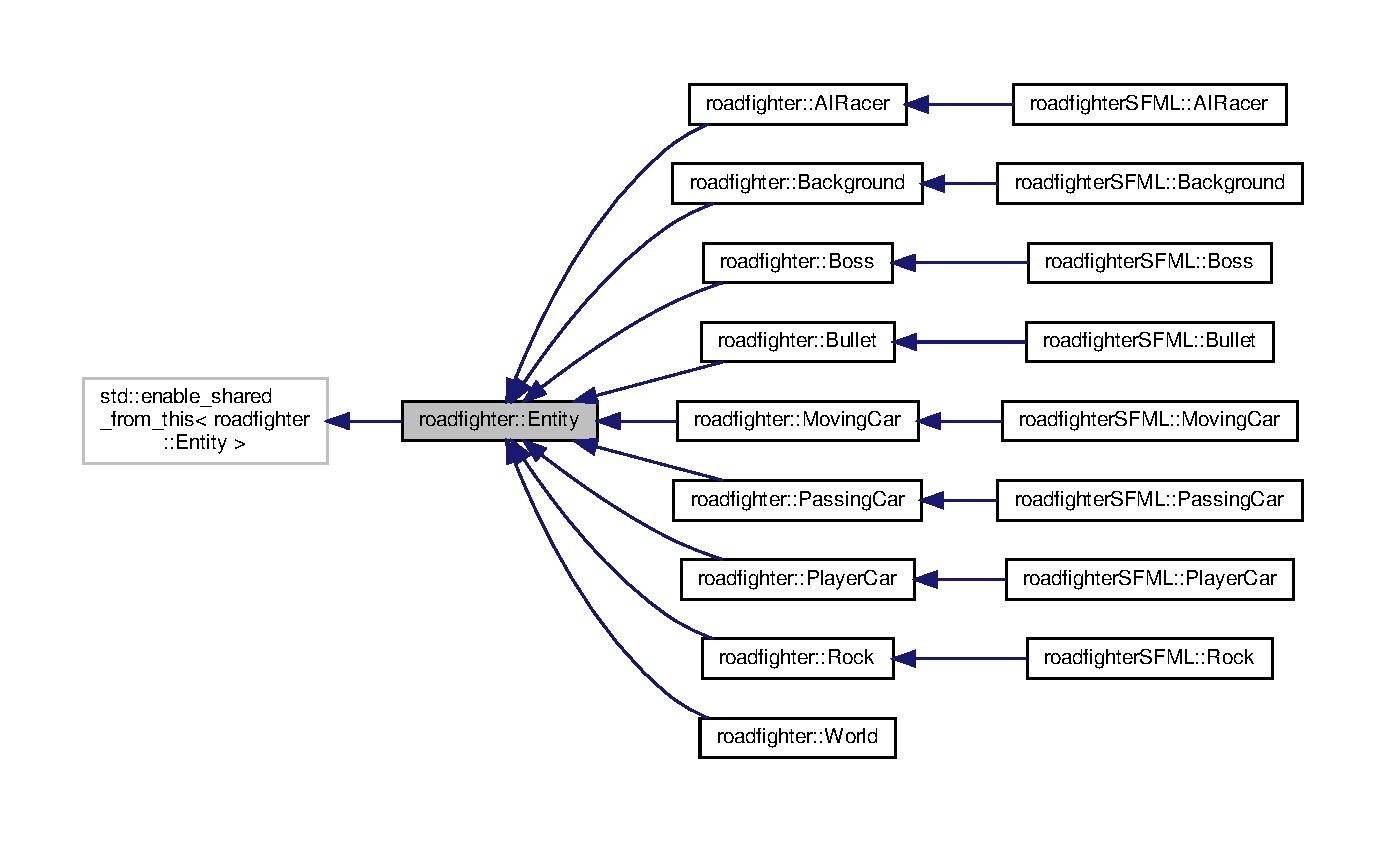
\includegraphics[width=350pt]{classroadfighter_1_1Entity__inherit__graph}
\end{center}
\end{figure}


Collaboration diagram for roadfighter\+:\+:Entity\+:\nopagebreak
\begin{figure}[H]
\begin{center}
\leavevmode
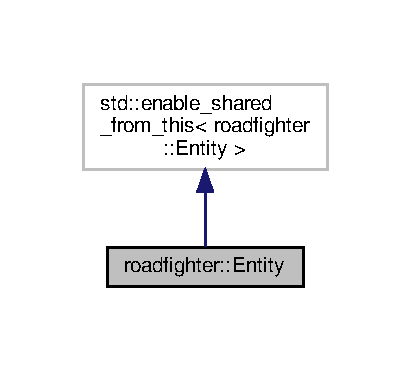
\includegraphics[width=197pt]{classroadfighter_1_1Entity__coll__graph}
\end{center}
\end{figure}
\subsection*{Public Member Functions}
\begin{DoxyCompactItemize}
\item 
virtual void \hyperlink{classroadfighter_1_1Entity_ac516f8005f969ad5a86c252e5a3640ee}{draw} ()=0
\item 
virtual void \hyperlink{classroadfighter_1_1Entity_a19cd353f12a3e8432acd6d5609137561}{update} ()=0
\item 
virtual void \hyperlink{classroadfighter_1_1Entity_a611ba56595dd2137d308876ba820cc09}{update} (int speed, std\+::shared\+\_\+ptr$<$ \hyperlink{classroadfighter_1_1Entity}{roadfighter\+::\+Entity} $>$ Player)=0
\item 
virtual int \hyperlink{classroadfighter_1_1Entity_ad3760184d764a61922e1db7d98501ee4}{get\+Speed} ()=0
\item 
virtual int \hyperlink{classroadfighter_1_1Entity_a08190b0b8e6a3fcdb42273d6096152ac}{Delete} ()=0
\item 
virtual void \hyperlink{classroadfighter_1_1Entity_a07e973f0fa941a69e749629716877692}{set\+Delete} (int del)=0
\item 
virtual bool \hyperlink{classroadfighter_1_1Entity_ad0ecaa0539db252e591da83814251509}{Shoot} ()=0
\item 
virtual std\+::shared\+\_\+ptr$<$ \hyperlink{structObjBox}{Obj\+Box} $>$ \hyperlink{classroadfighter_1_1Entity_af14340d04a725175a6d221f23c35fa0c}{get\+Objbox} ()=0
\end{DoxyCompactItemize}
\subsection*{Protected Attributes}
\begin{DoxyCompactItemize}
\item 
std\+::shared\+\_\+ptr$<$ \hyperlink{classConfigData}{Config\+Data} $>$ \hyperlink{classroadfighter_1_1Entity_ab69d36ac1aea7450bf4f443a17af58c7}{Config}
\end{DoxyCompactItemize}


\subsection{Detailed Description}
Holds all the entities that can exist in the game most are splitted in a logic and S\+F\+ML part except for the world 

\subsection{Member Function Documentation}
\mbox{\Hypertarget{classroadfighter_1_1Entity_a08190b0b8e6a3fcdb42273d6096152ac}\label{classroadfighter_1_1Entity_a08190b0b8e6a3fcdb42273d6096152ac}} 
\index{roadfighter\+::\+Entity@{roadfighter\+::\+Entity}!Delete@{Delete}}
\index{Delete@{Delete}!roadfighter\+::\+Entity@{roadfighter\+::\+Entity}}
\subsubsection{\texorpdfstring{Delete()}{Delete()}}
{\footnotesize\ttfamily virtual int roadfighter\+::\+Entity\+::\+Delete (\begin{DoxyParamCaption}{ }\end{DoxyParamCaption})\hspace{0.3cm}{\ttfamily [pure virtual]}}

Returns a certain value to determine the delete status 0 = nothing, 1 = delete, 2 = respawn \begin{DoxyReturn}{Returns}

\end{DoxyReturn}


Implemented in \hyperlink{classroadfighter_1_1World_a2db677b750afc0bf4f706f4cd930cb02}{roadfighter\+::\+World}, \hyperlink{classroadfighter_1_1PlayerCar_a1c4a181eee7a89315680eca4892ebc32}{roadfighter\+::\+Player\+Car}, \hyperlink{classroadfighter_1_1Boss_a8ffadaa85b61447da023c043d3d2dcc9}{roadfighter\+::\+Boss}, \hyperlink{classroadfighter_1_1AIRacer_af6fe47885c72aeddd02d13e136f4790f}{roadfighter\+::\+A\+I\+Racer}, \hyperlink{classroadfighter_1_1Background_a6541d509079dfa940d9f7ec2ab706963}{roadfighter\+::\+Background}, \hyperlink{classroadfighter_1_1MovingCar_a97196aa72de773ac88d1df99c47a5367}{roadfighter\+::\+Moving\+Car}, \hyperlink{classroadfighter_1_1PassingCar_a1a2838de0992a6e46793d0fe0f128b36}{roadfighter\+::\+Passing\+Car}, \hyperlink{classroadfighter_1_1Rock_a7ac4934b909f1f988b64ac8afc84ea85}{roadfighter\+::\+Rock}, and \hyperlink{classroadfighter_1_1Bullet_a011f2271222e0fa9bcf25193c2b94932}{roadfighter\+::\+Bullet}.

\mbox{\Hypertarget{classroadfighter_1_1Entity_ac516f8005f969ad5a86c252e5a3640ee}\label{classroadfighter_1_1Entity_ac516f8005f969ad5a86c252e5a3640ee}} 
\index{roadfighter\+::\+Entity@{roadfighter\+::\+Entity}!draw@{draw}}
\index{draw@{draw}!roadfighter\+::\+Entity@{roadfighter\+::\+Entity}}
\subsubsection{\texorpdfstring{draw()}{draw()}}
{\footnotesize\ttfamily virtual void roadfighter\+::\+Entity\+::draw (\begin{DoxyParamCaption}{ }\end{DoxyParamCaption})\hspace{0.3cm}{\ttfamily [pure virtual]}}

Draw an object 

Implemented in \hyperlink{classroadfighter_1_1World_a90534263a154d6d7c1e8aef4e0138881}{roadfighter\+::\+World}, \hyperlink{classroadfighterSFML_1_1Background_a02b49875cfb5d0c77d30c2ddbc05c46f}{roadfighter\+S\+F\+M\+L\+::\+Background}, \hyperlink{classroadfighterSFML_1_1PassingCar_ae8d3cff5198ad85dde5ab864b0528337}{roadfighter\+S\+F\+M\+L\+::\+Passing\+Car}, \hyperlink{classroadfighterSFML_1_1MovingCar_afff9b85787e5af092cce59be3370a683}{roadfighter\+S\+F\+M\+L\+::\+Moving\+Car}, \hyperlink{classroadfighterSFML_1_1PlayerCar_a9676cb8164bbc20f2ddedccf73ec5ef8}{roadfighter\+S\+F\+M\+L\+::\+Player\+Car}, \hyperlink{classroadfighterSFML_1_1AIRacer_a50d966c9d59e09a155d69e2c2296fb4e}{roadfighter\+S\+F\+M\+L\+::\+A\+I\+Racer}, \hyperlink{classroadfighterSFML_1_1Boss_a73041bc4cc4446fcf4605abe1052aa03}{roadfighter\+S\+F\+M\+L\+::\+Boss}, \hyperlink{classroadfighterSFML_1_1Bullet_a37d6977eace695d237c8859a0bcd413c}{roadfighter\+S\+F\+M\+L\+::\+Bullet}, and \hyperlink{classroadfighterSFML_1_1Rock_a7416f3e77114d38994d0de4d78e9f403}{roadfighter\+S\+F\+M\+L\+::\+Rock}.

\mbox{\Hypertarget{classroadfighter_1_1Entity_af14340d04a725175a6d221f23c35fa0c}\label{classroadfighter_1_1Entity_af14340d04a725175a6d221f23c35fa0c}} 
\index{roadfighter\+::\+Entity@{roadfighter\+::\+Entity}!get\+Objbox@{get\+Objbox}}
\index{get\+Objbox@{get\+Objbox}!roadfighter\+::\+Entity@{roadfighter\+::\+Entity}}
\subsubsection{\texorpdfstring{get\+Objbox()}{getObjbox()}}
{\footnotesize\ttfamily virtual std\+::shared\+\_\+ptr$<$\hyperlink{structObjBox}{Obj\+Box}$>$ roadfighter\+::\+Entity\+::get\+Objbox (\begin{DoxyParamCaption}{ }\end{DoxyParamCaption})\hspace{0.3cm}{\ttfamily [pure virtual]}}

Return the object box of an object \begin{DoxyReturn}{Returns}

\end{DoxyReturn}


Implemented in \hyperlink{classroadfighter_1_1World_a8825a89883229773abb09bb05ee89714}{roadfighter\+::\+World}, \hyperlink{classroadfighter_1_1PlayerCar_ac0b95a6ef2829905ad4717a52b7cb5eb}{roadfighter\+::\+Player\+Car}, \hyperlink{classroadfighter_1_1Boss_a3cf68c683f4352908eab55fc6ee29e9e}{roadfighter\+::\+Boss}, \hyperlink{classroadfighter_1_1AIRacer_a597fa189f88db3ca1534ddf24bb51c22}{roadfighter\+::\+A\+I\+Racer}, \hyperlink{classroadfighter_1_1Background_af25322839a52bc232266cceb2a85dd7d}{roadfighter\+::\+Background}, \hyperlink{classroadfighter_1_1MovingCar_a8b744958eaba45078e98fad4ac6821c3}{roadfighter\+::\+Moving\+Car}, \hyperlink{classroadfighter_1_1PassingCar_aeee1f7e16dcef7adc0a4bea629b0d42b}{roadfighter\+::\+Passing\+Car}, \hyperlink{classroadfighter_1_1Rock_a286656165c7dd3cdf66945e47f6fa4c7}{roadfighter\+::\+Rock}, and \hyperlink{classroadfighter_1_1Bullet_a3e410865547614ec0470eb6ad18cc2c4}{roadfighter\+::\+Bullet}.

\mbox{\Hypertarget{classroadfighter_1_1Entity_ad3760184d764a61922e1db7d98501ee4}\label{classroadfighter_1_1Entity_ad3760184d764a61922e1db7d98501ee4}} 
\index{roadfighter\+::\+Entity@{roadfighter\+::\+Entity}!get\+Speed@{get\+Speed}}
\index{get\+Speed@{get\+Speed}!roadfighter\+::\+Entity@{roadfighter\+::\+Entity}}
\subsubsection{\texorpdfstring{get\+Speed()}{getSpeed()}}
{\footnotesize\ttfamily virtual int roadfighter\+::\+Entity\+::get\+Speed (\begin{DoxyParamCaption}{ }\end{DoxyParamCaption})\hspace{0.3cm}{\ttfamily [pure virtual]}}

Return the speed of an object \begin{DoxyReturn}{Returns}

\end{DoxyReturn}


Implemented in \hyperlink{classroadfighter_1_1PlayerCar_a642a825b604a407ae4711bdafd054b22}{roadfighter\+::\+Player\+Car}, \hyperlink{classroadfighter_1_1World_a0ec7ca6d1df344ec56cf55d6d436b24c}{roadfighter\+::\+World}, \hyperlink{classroadfighter_1_1Boss_a348151aa9aabb3baabf9a8cc0b6955cb}{roadfighter\+::\+Boss}, \hyperlink{classroadfighter_1_1AIRacer_a4fa90fd500b2e790fb50cc6f1505688f}{roadfighter\+::\+A\+I\+Racer}, \hyperlink{classroadfighter_1_1Background_acbeaa8438617d67f8069347000e185a1}{roadfighter\+::\+Background}, \hyperlink{classroadfighter_1_1MovingCar_a42bdd9382e7234ae79d6f5e582adee92}{roadfighter\+::\+Moving\+Car}, \hyperlink{classroadfighter_1_1PassingCar_afae62d9c6037d5ce8f74bb2e2ed363ac}{roadfighter\+::\+Passing\+Car}, \hyperlink{classroadfighter_1_1Rock_ab3f596c927c49ab4b159391dc7287192}{roadfighter\+::\+Rock}, and \hyperlink{classroadfighter_1_1Bullet_ad05d66d01f1f839e1f38c6f12a0b091b}{roadfighter\+::\+Bullet}.

\mbox{\Hypertarget{classroadfighter_1_1Entity_a07e973f0fa941a69e749629716877692}\label{classroadfighter_1_1Entity_a07e973f0fa941a69e749629716877692}} 
\index{roadfighter\+::\+Entity@{roadfighter\+::\+Entity}!set\+Delete@{set\+Delete}}
\index{set\+Delete@{set\+Delete}!roadfighter\+::\+Entity@{roadfighter\+::\+Entity}}
\subsubsection{\texorpdfstring{set\+Delete()}{setDelete()}}
{\footnotesize\ttfamily virtual void roadfighter\+::\+Entity\+::set\+Delete (\begin{DoxyParamCaption}\item[{int}]{del }\end{DoxyParamCaption})\hspace{0.3cm}{\ttfamily [pure virtual]}}

Set if an object must be deleted 
\begin{DoxyParams}{Parameters}
{\em del} & \\
\hline
\end{DoxyParams}


Implemented in \hyperlink{classroadfighter_1_1World_a78c860f6700cd7f8e47994c02e7fd181}{roadfighter\+::\+World}, \hyperlink{classroadfighter_1_1PlayerCar_a24401332a8585b0fcfbfd33df93021e0}{roadfighter\+::\+Player\+Car}, \hyperlink{classroadfighter_1_1Boss_a8e2d5737afc0df4bc8b8ad0ddc03f5b8}{roadfighter\+::\+Boss}, \hyperlink{classroadfighter_1_1AIRacer_a10823d4a02dbdad6d760020f8cee7afe}{roadfighter\+::\+A\+I\+Racer}, \hyperlink{classroadfighter_1_1Background_acb4cdc56872d164b297b5655124df54d}{roadfighter\+::\+Background}, \hyperlink{classroadfighter_1_1MovingCar_a2fd9123a7ee59d4796672ad79656e1b5}{roadfighter\+::\+Moving\+Car}, \hyperlink{classroadfighter_1_1PassingCar_aad1905fcb427945c3300840deedffb1d}{roadfighter\+::\+Passing\+Car}, \hyperlink{classroadfighter_1_1Rock_ae2cef1d49610edd8b0438b6c84fdabfd}{roadfighter\+::\+Rock}, and \hyperlink{classroadfighter_1_1Bullet_ac3be16d9ff7da992fc6c5bd641f6d8dc}{roadfighter\+::\+Bullet}.

\mbox{\Hypertarget{classroadfighter_1_1Entity_ad0ecaa0539db252e591da83814251509}\label{classroadfighter_1_1Entity_ad0ecaa0539db252e591da83814251509}} 
\index{roadfighter\+::\+Entity@{roadfighter\+::\+Entity}!Shoot@{Shoot}}
\index{Shoot@{Shoot}!roadfighter\+::\+Entity@{roadfighter\+::\+Entity}}
\subsubsection{\texorpdfstring{Shoot()}{Shoot()}}
{\footnotesize\ttfamily virtual bool roadfighter\+::\+Entity\+::\+Shoot (\begin{DoxyParamCaption}{ }\end{DoxyParamCaption})\hspace{0.3cm}{\ttfamily [pure virtual]}}

Return if an object must shoot \begin{DoxyReturn}{Returns}

\end{DoxyReturn}


Implemented in \hyperlink{classroadfighter_1_1World_ab168eec31ad01a882254c5522b354d22}{roadfighter\+::\+World}, \hyperlink{classroadfighter_1_1PlayerCar_af9e034824497fb287085be08c3995733}{roadfighter\+::\+Player\+Car}, \hyperlink{classroadfighter_1_1Boss_a794027599b17398ae72c65aa1837d864}{roadfighter\+::\+Boss}, \hyperlink{classroadfighter_1_1AIRacer_a9e1ce152093bd4f7deb676c443a7851a}{roadfighter\+::\+A\+I\+Racer}, \hyperlink{classroadfighter_1_1Background_a1482152bca4207b44f1ce1c2c5af5847}{roadfighter\+::\+Background}, \hyperlink{classroadfighter_1_1MovingCar_a5b7a6cf114fe26016434b2fcf3434d37}{roadfighter\+::\+Moving\+Car}, \hyperlink{classroadfighter_1_1PassingCar_a16df11cb6ac5ce29b733d1063490c95c}{roadfighter\+::\+Passing\+Car}, \hyperlink{classroadfighter_1_1Rock_a1bcf89f9c386a3b248033ba3f0329e9c}{roadfighter\+::\+Rock}, and \hyperlink{classroadfighter_1_1Bullet_a0c093704ce5b9c2f4237d6b5dd1cbd36}{roadfighter\+::\+Bullet}.

\mbox{\Hypertarget{classroadfighter_1_1Entity_a19cd353f12a3e8432acd6d5609137561}\label{classroadfighter_1_1Entity_a19cd353f12a3e8432acd6d5609137561}} 
\index{roadfighter\+::\+Entity@{roadfighter\+::\+Entity}!update@{update}}
\index{update@{update}!roadfighter\+::\+Entity@{roadfighter\+::\+Entity}}
\subsubsection{\texorpdfstring{update()}{update()}\hspace{0.1cm}{\footnotesize\ttfamily [1/2]}}
{\footnotesize\ttfamily virtual void roadfighter\+::\+Entity\+::update (\begin{DoxyParamCaption}{ }\end{DoxyParamCaption})\hspace{0.3cm}{\ttfamily [pure virtual]}}

Update an object 

Implemented in \hyperlink{classroadfighter_1_1PlayerCar_a47772fa1d9fcdba69f288112d5359acd}{roadfighter\+::\+Player\+Car}, \hyperlink{classroadfighter_1_1AIRacer_a92afd3d1bfcd290d3b012cbfe44d5a77}{roadfighter\+::\+A\+I\+Racer}, \hyperlink{classroadfighter_1_1World_af4988cdad9b54a049de1a29ff87679ec}{roadfighter\+::\+World}, \hyperlink{classroadfighter_1_1Boss_aa097f1f2e3fe76645233a4ba75ee6256}{roadfighter\+::\+Boss}, \hyperlink{classroadfighter_1_1Background_a6fa762ca6aa2f18918c1b715ae94395f}{roadfighter\+::\+Background}, \hyperlink{classroadfighter_1_1MovingCar_a06c6e2e0510707bdd7e4570b8f65241c}{roadfighter\+::\+Moving\+Car}, \hyperlink{classroadfighter_1_1PassingCar_a45276fb9270a145fed9a7827a9ab7a46}{roadfighter\+::\+Passing\+Car}, \hyperlink{classroadfighter_1_1Rock_a28d9c3334f54db88785696076a8b6c9c}{roadfighter\+::\+Rock}, \hyperlink{classroadfighter_1_1Bullet_aab45c1cb9088b11c17e7a238543d8006}{roadfighter\+::\+Bullet}, \hyperlink{classroadfighterSFML_1_1PlayerCar_a1fb9b80b068e689bef90cad28c53869c}{roadfighter\+S\+F\+M\+L\+::\+Player\+Car}, and \hyperlink{classroadfighterSFML_1_1AIRacer_aaecd91860a2ac61ef671000e311b7860}{roadfighter\+S\+F\+M\+L\+::\+A\+I\+Racer}.

\mbox{\Hypertarget{classroadfighter_1_1Entity_a611ba56595dd2137d308876ba820cc09}\label{classroadfighter_1_1Entity_a611ba56595dd2137d308876ba820cc09}} 
\index{roadfighter\+::\+Entity@{roadfighter\+::\+Entity}!update@{update}}
\index{update@{update}!roadfighter\+::\+Entity@{roadfighter\+::\+Entity}}
\subsubsection{\texorpdfstring{update()}{update()}\hspace{0.1cm}{\footnotesize\ttfamily [2/2]}}
{\footnotesize\ttfamily virtual void roadfighter\+::\+Entity\+::update (\begin{DoxyParamCaption}\item[{int}]{speed,  }\item[{std\+::shared\+\_\+ptr$<$ \hyperlink{classroadfighter_1_1Entity}{roadfighter\+::\+Entity} $>$}]{Player }\end{DoxyParamCaption})\hspace{0.3cm}{\ttfamily [pure virtual]}}

Updates the entity with the speed of the player and the player 
\begin{DoxyParams}{Parameters}
{\em speed} & \\
\hline
{\em Player} & \\
\hline
\end{DoxyParams}


Implemented in \hyperlink{classroadfighter_1_1PlayerCar_a65daed6d30d8b65f368779eaa43714e2}{roadfighter\+::\+Player\+Car}, \hyperlink{classroadfighter_1_1World_a8c26e9cb031b250cdc263623615c1891}{roadfighter\+::\+World}, \hyperlink{classroadfighter_1_1Boss_a1754fba639f122f50e3eeb55980008b2}{roadfighter\+::\+Boss}, \hyperlink{classroadfighter_1_1AIRacer_ab6156385195b3d40d44360d40aafa3a6}{roadfighter\+::\+A\+I\+Racer}, \hyperlink{classroadfighter_1_1Background_a881ed4d9e98e86ce7128c0fd18f82160}{roadfighter\+::\+Background}, \hyperlink{classroadfighter_1_1MovingCar_a62fbe61c5a1c1a1c0d376047ec1edcf2}{roadfighter\+::\+Moving\+Car}, \hyperlink{classroadfighter_1_1PassingCar_af0667cf430382117beb4669777905cc7}{roadfighter\+::\+Passing\+Car}, \hyperlink{classroadfighter_1_1Rock_af9817c01175d300ca7be67e2b5e3952e}{roadfighter\+::\+Rock}, and \hyperlink{classroadfighter_1_1Bullet_a9027c832dce3cd2839192255e0dbf301}{roadfighter\+::\+Bullet}.



\subsection{Member Data Documentation}
\mbox{\Hypertarget{classroadfighter_1_1Entity_ab69d36ac1aea7450bf4f443a17af58c7}\label{classroadfighter_1_1Entity_ab69d36ac1aea7450bf4f443a17af58c7}} 
\index{roadfighter\+::\+Entity@{roadfighter\+::\+Entity}!Config@{Config}}
\index{Config@{Config}!roadfighter\+::\+Entity@{roadfighter\+::\+Entity}}
\subsubsection{\texorpdfstring{Config}{Config}}
{\footnotesize\ttfamily std\+::shared\+\_\+ptr$<$\hyperlink{classConfigData}{Config\+Data}$>$ roadfighter\+::\+Entity\+::\+Config\hspace{0.3cm}{\ttfamily [protected]}}

Configuration data 

The documentation for this class was generated from the following file\+:\begin{DoxyCompactItemize}
\item 
roadfighter/Entity.\+h\end{DoxyCompactItemize}

\hypertarget{classroadfighter_1_1EntityFactory}{}\section{roadfighter\+:\+:Entity\+Factory Class Reference}
\label{classroadfighter_1_1EntityFactory}\index{roadfighter\+::\+Entity\+Factory@{roadfighter\+::\+Entity\+Factory}}


{\ttfamily \#include $<$Entity\+Factory.\+h$>$}



Inheritance diagram for roadfighter\+:\+:Entity\+Factory\+:\nopagebreak
\begin{figure}[H]
\begin{center}
\leavevmode
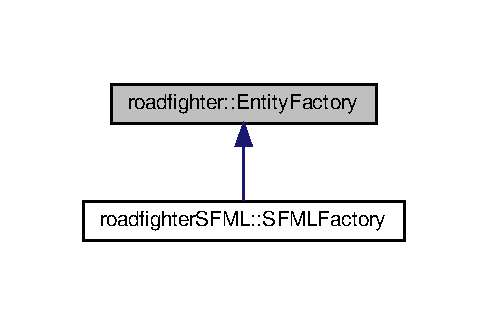
\includegraphics[width=234pt]{classroadfighter_1_1EntityFactory__inherit__graph}
\end{center}
\end{figure}
\subsection*{Public Member Functions}
\begin{DoxyCompactItemize}
\item 
virtual std\+::shared\+\_\+ptr$<$ \hyperlink{classroadfighter_1_1Entity}{roadfighter\+::\+Entity} $>$ \hyperlink{classroadfighter_1_1EntityFactory_a8fefd94a197c87544805461761fc111c}{create\+Player\+Car} (int level)=0
\item 
virtual std\+::shared\+\_\+ptr$<$ \hyperlink{classroadfighter_1_1Entity}{roadfighter\+::\+Entity} $>$ \hyperlink{classroadfighter_1_1EntityFactory_ab3586917a6ef9d3a92b825f908132e02}{create\+Background} (int i)=0
\item 
virtual std\+::shared\+\_\+ptr$<$ \hyperlink{classroadfighter_1_1Entity}{roadfighter\+::\+Entity} $>$ \hyperlink{classroadfighter_1_1EntityFactory_ab318794f4effc0c2195fae5da267d900}{create\+Passing\+Car} (double i)=0
\item 
virtual std\+::shared\+\_\+ptr$<$ \hyperlink{classroadfighter_1_1Entity}{roadfighter\+::\+Entity} $>$ \hyperlink{classroadfighter_1_1EntityFactory_a2d4319aef20024f83e7c3189e92c89e1}{create\+Bullet} (double first, double second)=0
\item 
virtual std\+::shared\+\_\+ptr$<$ \hyperlink{classroadfighter_1_1Entity}{roadfighter\+::\+Entity} $>$ \hyperlink{classroadfighter_1_1EntityFactory_a3bcb7e8b8ca62628c842962cfbba50be}{create\+Rock} (double i)=0
\item 
virtual std\+::shared\+\_\+ptr$<$ \hyperlink{classroadfighter_1_1Entity}{roadfighter\+::\+Entity} $>$ \hyperlink{classroadfighter_1_1EntityFactory_a53cc68cc3f7365e4ded258ea9b281b45}{create\+Moving\+Car} (double i)=0
\item 
virtual std\+::shared\+\_\+ptr$<$ \hyperlink{classroadfighter_1_1AIRacer}{roadfighter\+::\+A\+I\+Racer} $>$ \hyperlink{classroadfighter_1_1EntityFactory_ae50d1b8cbf0b63dfbedca775781fbda0}{create\+AI} ()=0
\item 
virtual std\+::shared\+\_\+ptr$<$ \hyperlink{classroadfighter_1_1Boss}{roadfighter\+::\+Boss} $>$ \hyperlink{classroadfighter_1_1EntityFactory_ae7a09423660432e744ed35f5f04b0931}{create\+Boss} ()=0
\end{DoxyCompactItemize}


\subsection{Detailed Description}
Factory for creating entities 

\subsection{Member Function Documentation}
\mbox{\Hypertarget{classroadfighter_1_1EntityFactory_ae50d1b8cbf0b63dfbedca775781fbda0}\label{classroadfighter_1_1EntityFactory_ae50d1b8cbf0b63dfbedca775781fbda0}} 
\index{roadfighter\+::\+Entity\+Factory@{roadfighter\+::\+Entity\+Factory}!create\+AI@{create\+AI}}
\index{create\+AI@{create\+AI}!roadfighter\+::\+Entity\+Factory@{roadfighter\+::\+Entity\+Factory}}
\subsubsection{\texorpdfstring{create\+A\+I()}{createAI()}}
{\footnotesize\ttfamily virtual std\+::shared\+\_\+ptr$<$\hyperlink{classroadfighter_1_1AIRacer}{roadfighter\+::\+A\+I\+Racer}$>$ roadfighter\+::\+Entity\+Factory\+::create\+AI (\begin{DoxyParamCaption}{ }\end{DoxyParamCaption})\hspace{0.3cm}{\ttfamily [pure virtual]}}

Create an ai racer \begin{DoxyReturn}{Returns}

\end{DoxyReturn}


Implemented in \hyperlink{classroadfighterSFML_1_1SFMLFactory_a977a002d878172e485bea8679c136d76}{roadfighter\+S\+F\+M\+L\+::\+S\+F\+M\+L\+Factory}.

\mbox{\Hypertarget{classroadfighter_1_1EntityFactory_ab3586917a6ef9d3a92b825f908132e02}\label{classroadfighter_1_1EntityFactory_ab3586917a6ef9d3a92b825f908132e02}} 
\index{roadfighter\+::\+Entity\+Factory@{roadfighter\+::\+Entity\+Factory}!create\+Background@{create\+Background}}
\index{create\+Background@{create\+Background}!roadfighter\+::\+Entity\+Factory@{roadfighter\+::\+Entity\+Factory}}
\subsubsection{\texorpdfstring{create\+Background()}{createBackground()}}
{\footnotesize\ttfamily virtual std\+::shared\+\_\+ptr$<$\hyperlink{classroadfighter_1_1Entity}{roadfighter\+::\+Entity}$>$ roadfighter\+::\+Entity\+Factory\+::create\+Background (\begin{DoxyParamCaption}\item[{int}]{i }\end{DoxyParamCaption})\hspace{0.3cm}{\ttfamily [pure virtual]}}

Create a background \begin{DoxyReturn}{Returns}

\end{DoxyReturn}


Implemented in \hyperlink{classroadfighterSFML_1_1SFMLFactory_a18a78a7113edf49647f727105329f605}{roadfighter\+S\+F\+M\+L\+::\+S\+F\+M\+L\+Factory}.

\mbox{\Hypertarget{classroadfighter_1_1EntityFactory_ae7a09423660432e744ed35f5f04b0931}\label{classroadfighter_1_1EntityFactory_ae7a09423660432e744ed35f5f04b0931}} 
\index{roadfighter\+::\+Entity\+Factory@{roadfighter\+::\+Entity\+Factory}!create\+Boss@{create\+Boss}}
\index{create\+Boss@{create\+Boss}!roadfighter\+::\+Entity\+Factory@{roadfighter\+::\+Entity\+Factory}}
\subsubsection{\texorpdfstring{create\+Boss()}{createBoss()}}
{\footnotesize\ttfamily virtual std\+::shared\+\_\+ptr$<$\hyperlink{classroadfighter_1_1Boss}{roadfighter\+::\+Boss}$>$ roadfighter\+::\+Entity\+Factory\+::create\+Boss (\begin{DoxyParamCaption}{ }\end{DoxyParamCaption})\hspace{0.3cm}{\ttfamily [pure virtual]}}

Create the boss \begin{DoxyReturn}{Returns}

\end{DoxyReturn}


Implemented in \hyperlink{classroadfighterSFML_1_1SFMLFactory_a86f4fed282eebc1556ed1134e7ad7e13}{roadfighter\+S\+F\+M\+L\+::\+S\+F\+M\+L\+Factory}.

\mbox{\Hypertarget{classroadfighter_1_1EntityFactory_a2d4319aef20024f83e7c3189e92c89e1}\label{classroadfighter_1_1EntityFactory_a2d4319aef20024f83e7c3189e92c89e1}} 
\index{roadfighter\+::\+Entity\+Factory@{roadfighter\+::\+Entity\+Factory}!create\+Bullet@{create\+Bullet}}
\index{create\+Bullet@{create\+Bullet}!roadfighter\+::\+Entity\+Factory@{roadfighter\+::\+Entity\+Factory}}
\subsubsection{\texorpdfstring{create\+Bullet()}{createBullet()}}
{\footnotesize\ttfamily virtual std\+::shared\+\_\+ptr$<$\hyperlink{classroadfighter_1_1Entity}{roadfighter\+::\+Entity}$>$ roadfighter\+::\+Entity\+Factory\+::create\+Bullet (\begin{DoxyParamCaption}\item[{double}]{first,  }\item[{double}]{second }\end{DoxyParamCaption})\hspace{0.3cm}{\ttfamily [pure virtual]}}

Create a bullet 
\begin{DoxyParams}{Parameters}
{\em first} & = x position of car \\
\hline
{\em second} & = y position of car \\
\hline
\end{DoxyParams}
\begin{DoxyReturn}{Returns}

\end{DoxyReturn}


Implemented in \hyperlink{classroadfighterSFML_1_1SFMLFactory_aac2ed62453b201da7d124947b6cd475b}{roadfighter\+S\+F\+M\+L\+::\+S\+F\+M\+L\+Factory}.

\mbox{\Hypertarget{classroadfighter_1_1EntityFactory_a53cc68cc3f7365e4ded258ea9b281b45}\label{classroadfighter_1_1EntityFactory_a53cc68cc3f7365e4ded258ea9b281b45}} 
\index{roadfighter\+::\+Entity\+Factory@{roadfighter\+::\+Entity\+Factory}!create\+Moving\+Car@{create\+Moving\+Car}}
\index{create\+Moving\+Car@{create\+Moving\+Car}!roadfighter\+::\+Entity\+Factory@{roadfighter\+::\+Entity\+Factory}}
\subsubsection{\texorpdfstring{create\+Moving\+Car()}{createMovingCar()}}
{\footnotesize\ttfamily virtual std\+::shared\+\_\+ptr$<$\hyperlink{classroadfighter_1_1Entity}{roadfighter\+::\+Entity}$>$ roadfighter\+::\+Entity\+Factory\+::create\+Moving\+Car (\begin{DoxyParamCaption}\item[{double}]{i }\end{DoxyParamCaption})\hspace{0.3cm}{\ttfamily [pure virtual]}}

create a moving car 
\begin{DoxyParams}{Parameters}
{\em i} & = random position \\
\hline
\end{DoxyParams}
\begin{DoxyReturn}{Returns}

\end{DoxyReturn}


Implemented in \hyperlink{classroadfighterSFML_1_1SFMLFactory_aa1aeba2d2613b784d9da5f6fd3109154}{roadfighter\+S\+F\+M\+L\+::\+S\+F\+M\+L\+Factory}.

\mbox{\Hypertarget{classroadfighter_1_1EntityFactory_ab318794f4effc0c2195fae5da267d900}\label{classroadfighter_1_1EntityFactory_ab318794f4effc0c2195fae5da267d900}} 
\index{roadfighter\+::\+Entity\+Factory@{roadfighter\+::\+Entity\+Factory}!create\+Passing\+Car@{create\+Passing\+Car}}
\index{create\+Passing\+Car@{create\+Passing\+Car}!roadfighter\+::\+Entity\+Factory@{roadfighter\+::\+Entity\+Factory}}
\subsubsection{\texorpdfstring{create\+Passing\+Car()}{createPassingCar()}}
{\footnotesize\ttfamily virtual std\+::shared\+\_\+ptr$<$\hyperlink{classroadfighter_1_1Entity}{roadfighter\+::\+Entity}$>$ roadfighter\+::\+Entity\+Factory\+::create\+Passing\+Car (\begin{DoxyParamCaption}\item[{double}]{i }\end{DoxyParamCaption})\hspace{0.3cm}{\ttfamily [pure virtual]}}

Create a passing car 
\begin{DoxyParams}{Parameters}
{\em i} & = random position \\
\hline
\end{DoxyParams}
\begin{DoxyReturn}{Returns}

\end{DoxyReturn}


Implemented in \hyperlink{classroadfighterSFML_1_1SFMLFactory_a9960aec21f58babf83857cc400dad8fe}{roadfighter\+S\+F\+M\+L\+::\+S\+F\+M\+L\+Factory}.

\mbox{\Hypertarget{classroadfighter_1_1EntityFactory_a8fefd94a197c87544805461761fc111c}\label{classroadfighter_1_1EntityFactory_a8fefd94a197c87544805461761fc111c}} 
\index{roadfighter\+::\+Entity\+Factory@{roadfighter\+::\+Entity\+Factory}!create\+Player\+Car@{create\+Player\+Car}}
\index{create\+Player\+Car@{create\+Player\+Car}!roadfighter\+::\+Entity\+Factory@{roadfighter\+::\+Entity\+Factory}}
\subsubsection{\texorpdfstring{create\+Player\+Car()}{createPlayerCar()}}
{\footnotesize\ttfamily virtual std\+::shared\+\_\+ptr$<$\hyperlink{classroadfighter_1_1Entity}{roadfighter\+::\+Entity}$>$ roadfighter\+::\+Entity\+Factory\+::create\+Player\+Car (\begin{DoxyParamCaption}\item[{int}]{level }\end{DoxyParamCaption})\hspace{0.3cm}{\ttfamily [pure virtual]}}

Create a playercar \begin{DoxyReturn}{Returns}

\end{DoxyReturn}


Implemented in \hyperlink{classroadfighterSFML_1_1SFMLFactory_acb966ae41ef0a928c4adc34b4c97cedb}{roadfighter\+S\+F\+M\+L\+::\+S\+F\+M\+L\+Factory}.

\mbox{\Hypertarget{classroadfighter_1_1EntityFactory_a3bcb7e8b8ca62628c842962cfbba50be}\label{classroadfighter_1_1EntityFactory_a3bcb7e8b8ca62628c842962cfbba50be}} 
\index{roadfighter\+::\+Entity\+Factory@{roadfighter\+::\+Entity\+Factory}!create\+Rock@{create\+Rock}}
\index{create\+Rock@{create\+Rock}!roadfighter\+::\+Entity\+Factory@{roadfighter\+::\+Entity\+Factory}}
\subsubsection{\texorpdfstring{create\+Rock()}{createRock()}}
{\footnotesize\ttfamily virtual std\+::shared\+\_\+ptr$<$\hyperlink{classroadfighter_1_1Entity}{roadfighter\+::\+Entity}$>$ roadfighter\+::\+Entity\+Factory\+::create\+Rock (\begin{DoxyParamCaption}\item[{double}]{i }\end{DoxyParamCaption})\hspace{0.3cm}{\ttfamily [pure virtual]}}

create a rock 
\begin{DoxyParams}{Parameters}
{\em i} & = position \\
\hline
\end{DoxyParams}
\begin{DoxyReturn}{Returns}

\end{DoxyReturn}


Implemented in \hyperlink{classroadfighterSFML_1_1SFMLFactory_ace05bdfcf9fc4f1ca7b9fc6f840b7a12}{roadfighter\+S\+F\+M\+L\+::\+S\+F\+M\+L\+Factory}.



The documentation for this class was generated from the following file\+:\begin{DoxyCompactItemize}
\item 
roadfighter/Entity\+Factory.\+h\end{DoxyCompactItemize}

\hypertarget{classFileError}{}\section{File\+Error Class Reference}
\label{classFileError}\index{File\+Error@{File\+Error}}


{\ttfamily \#include $<$File\+Error.\+h$>$}



Inheritance diagram for File\+Error\+:\nopagebreak
\begin{figure}[H]
\begin{center}
\leavevmode
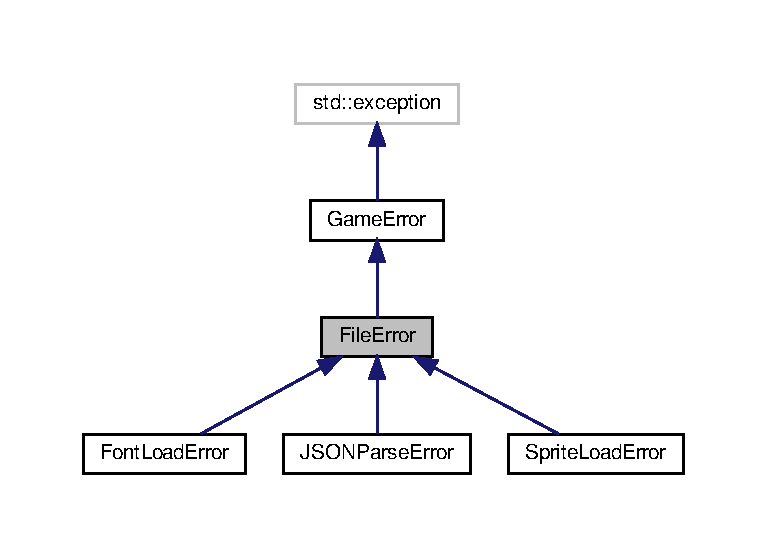
\includegraphics[width=350pt]{classFileError__inherit__graph}
\end{center}
\end{figure}


Collaboration diagram for File\+Error\+:\nopagebreak
\begin{figure}[H]
\begin{center}
\leavevmode
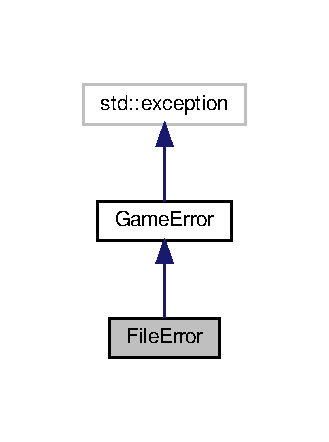
\includegraphics[width=158pt]{classFileError__coll__graph}
\end{center}
\end{figure}
\subsection*{Public Member Functions}
\begin{DoxyCompactItemize}
\item 
\hyperlink{classFileError_a8330c1e4ec86bfae59e4d9e96b2be59b}{File\+Error} (const char $\ast$\hyperlink{classFileError_a0ea1cc225bf7f8fa47aa0cfa0c2ba685}{file})
\item 
virtual const char $\ast$ \hyperlink{classFileError_a40918f5dda2ee7063bba81d286392cdd}{file\+Path} () const noexcept=0
\end{DoxyCompactItemize}
\subsection*{Protected Attributes}
\begin{DoxyCompactItemize}
\item 
const char $\ast$ \hyperlink{classFileError_a0ea1cc225bf7f8fa47aa0cfa0c2ba685}{file}
\end{DoxyCompactItemize}


\subsection{Detailed Description}
class that acts as parent class for errors that occur when loading or using files 

\subsection{Constructor \& Destructor Documentation}
\mbox{\Hypertarget{classFileError_a8330c1e4ec86bfae59e4d9e96b2be59b}\label{classFileError_a8330c1e4ec86bfae59e4d9e96b2be59b}} 
\index{File\+Error@{File\+Error}!File\+Error@{File\+Error}}
\index{File\+Error@{File\+Error}!File\+Error@{File\+Error}}
\subsubsection{\texorpdfstring{File\+Error()}{FileError()}}
{\footnotesize\ttfamily File\+Error\+::\+File\+Error (\begin{DoxyParamCaption}\item[{const char $\ast$}]{file }\end{DoxyParamCaption})}

Constructor for a file error with the file that caused the error 
\begin{DoxyParams}{Parameters}
{\em file} & \\
\hline
\end{DoxyParams}


\subsection{Member Function Documentation}
\mbox{\Hypertarget{classFileError_a40918f5dda2ee7063bba81d286392cdd}\label{classFileError_a40918f5dda2ee7063bba81d286392cdd}} 
\index{File\+Error@{File\+Error}!file\+Path@{file\+Path}}
\index{file\+Path@{file\+Path}!File\+Error@{File\+Error}}
\subsubsection{\texorpdfstring{file\+Path()}{filePath()}}
{\footnotesize\ttfamily virtual const char$\ast$ File\+Error\+::file\+Path (\begin{DoxyParamCaption}{ }\end{DoxyParamCaption}) const\hspace{0.3cm}{\ttfamily [pure virtual]}, {\ttfamily [noexcept]}}

Return the file that caused the error \begin{DoxyReturn}{Returns}

\end{DoxyReturn}


Implemented in \hyperlink{classFontLoadError_aa1b4295ca60b389717e40fcbf723fb83}{Font\+Load\+Error}, \hyperlink{classSpriteLoadError_aa6c6ca97b781b8045eb4271aad6aa6d1}{Sprite\+Load\+Error}, and \hyperlink{classJSONParseError_a24c5c1358b6ae6c96b30ebaa96e0a30b}{J\+S\+O\+N\+Parse\+Error}.



\subsection{Member Data Documentation}
\mbox{\Hypertarget{classFileError_a0ea1cc225bf7f8fa47aa0cfa0c2ba685}\label{classFileError_a0ea1cc225bf7f8fa47aa0cfa0c2ba685}} 
\index{File\+Error@{File\+Error}!file@{file}}
\index{file@{file}!File\+Error@{File\+Error}}
\subsubsection{\texorpdfstring{file}{file}}
{\footnotesize\ttfamily const char$\ast$ File\+Error\+::file\hspace{0.3cm}{\ttfamily [protected]}}

File that caused the error 

The documentation for this class was generated from the following files\+:\begin{DoxyCompactItemize}
\item 
Exception\+\_\+class/File\+Error.\+h\item 
Exception\+\_\+class/File\+Error.\+cpp\end{DoxyCompactItemize}

\hypertarget{classFontLoadError}{}\section{Font\+Load\+Error Class Reference}
\label{classFontLoadError}\index{Font\+Load\+Error@{Font\+Load\+Error}}


{\ttfamily \#include $<$Font\+Load\+Error.\+h$>$}



Inheritance diagram for Font\+Load\+Error\+:\nopagebreak
\begin{figure}[H]
\begin{center}
\leavevmode
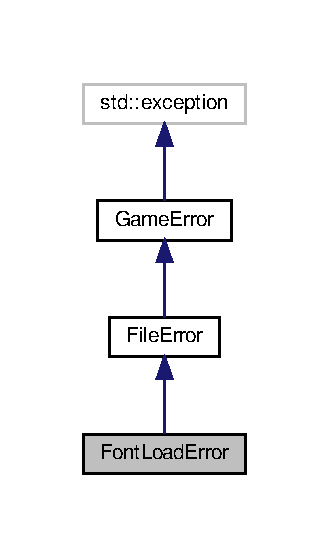
\includegraphics[width=158pt]{classFontLoadError__inherit__graph}
\end{center}
\end{figure}


Collaboration diagram for Font\+Load\+Error\+:\nopagebreak
\begin{figure}[H]
\begin{center}
\leavevmode
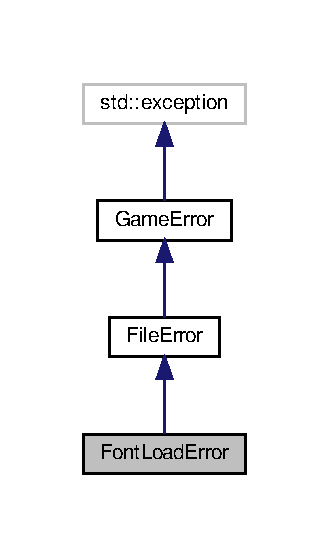
\includegraphics[width=158pt]{classFontLoadError__coll__graph}
\end{center}
\end{figure}
\subsection*{Public Member Functions}
\begin{DoxyCompactItemize}
\item 
const char $\ast$ \hyperlink{classFontLoadError_a523f16150eb19d25ed5692512e6952f5}{what} () const noexcept override
\item 
\hyperlink{classFontLoadError_a2d9e45a31deb3f088ce7d8f26381723d}{Font\+Load\+Error} (const char $\ast$\hyperlink{classFileError_a0ea1cc225bf7f8fa47aa0cfa0c2ba685}{file})
\item 
const char $\ast$ \hyperlink{classFontLoadError_aa1b4295ca60b389717e40fcbf723fb83}{file\+Path} () const noexcept override
\end{DoxyCompactItemize}
\subsection*{Additional Inherited Members}


\subsection{Detailed Description}
Error that appears when failing to load a font 

\subsection{Constructor \& Destructor Documentation}
\mbox{\Hypertarget{classFontLoadError_a2d9e45a31deb3f088ce7d8f26381723d}\label{classFontLoadError_a2d9e45a31deb3f088ce7d8f26381723d}} 
\index{Font\+Load\+Error@{Font\+Load\+Error}!Font\+Load\+Error@{Font\+Load\+Error}}
\index{Font\+Load\+Error@{Font\+Load\+Error}!Font\+Load\+Error@{Font\+Load\+Error}}
\subsubsection{\texorpdfstring{Font\+Load\+Error()}{FontLoadError()}}
{\footnotesize\ttfamily Font\+Load\+Error\+::\+Font\+Load\+Error (\begin{DoxyParamCaption}\item[{const char $\ast$}]{file }\end{DoxyParamCaption})}

Constructor with the file that caused the error 
\begin{DoxyParams}{Parameters}
{\em file} & \\
\hline
\end{DoxyParams}


\subsection{Member Function Documentation}
\mbox{\Hypertarget{classFontLoadError_aa1b4295ca60b389717e40fcbf723fb83}\label{classFontLoadError_aa1b4295ca60b389717e40fcbf723fb83}} 
\index{Font\+Load\+Error@{Font\+Load\+Error}!file\+Path@{file\+Path}}
\index{file\+Path@{file\+Path}!Font\+Load\+Error@{Font\+Load\+Error}}
\subsubsection{\texorpdfstring{file\+Path()}{filePath()}}
{\footnotesize\ttfamily const char $\ast$ Font\+Load\+Error\+::file\+Path (\begin{DoxyParamCaption}{ }\end{DoxyParamCaption}) const\hspace{0.3cm}{\ttfamily [override]}, {\ttfamily [virtual]}, {\ttfamily [noexcept]}}

return the file that caused the error \begin{DoxyReturn}{Returns}

\end{DoxyReturn}


Implements \hyperlink{classFileError_a40918f5dda2ee7063bba81d286392cdd}{File\+Error}.

\mbox{\Hypertarget{classFontLoadError_a523f16150eb19d25ed5692512e6952f5}\label{classFontLoadError_a523f16150eb19d25ed5692512e6952f5}} 
\index{Font\+Load\+Error@{Font\+Load\+Error}!what@{what}}
\index{what@{what}!Font\+Load\+Error@{Font\+Load\+Error}}
\subsubsection{\texorpdfstring{what()}{what()}}
{\footnotesize\ttfamily const char $\ast$ Font\+Load\+Error\+::what (\begin{DoxyParamCaption}{ }\end{DoxyParamCaption}) const\hspace{0.3cm}{\ttfamily [override]}, {\ttfamily [virtual]}, {\ttfamily [noexcept]}}

Return the error message \begin{DoxyReturn}{Returns}

\end{DoxyReturn}


Implements \hyperlink{classGameError_afbe93d6a2023f2824be2733aff9e86cb}{Game\+Error}.



The documentation for this class was generated from the following files\+:\begin{DoxyCompactItemize}
\item 
Exception\+\_\+class/Font\+Load\+Error.\+h\item 
Exception\+\_\+class/Font\+Load\+Error.\+cpp\end{DoxyCompactItemize}

\hypertarget{classGame}{}\section{Game Class Reference}
\label{classGame}\index{Game@{Game}}


{\ttfamily \#include $<$Game.\+h$>$}

\subsection*{Public Member Functions}
\begin{DoxyCompactItemize}
\item 
\hyperlink{classGame_ad59df6562a58a614fda24622d3715b65}{Game} ()
\item 
void \hyperlink{classGame_a1ab78f5ed0d5ea879157357cf2fb2afa}{run} ()
\item 
void \hyperlink{classGame_ae878cc28aa5519f8ba8e1ab6d3a33d25}{Parse} (int level)
\end{DoxyCompactItemize}


\subsection{Detailed Description}
Runs the game and holds the information of the window and world that need to be displayed 

\subsection{Constructor \& Destructor Documentation}
\mbox{\Hypertarget{classGame_ad59df6562a58a614fda24622d3715b65}\label{classGame_ad59df6562a58a614fda24622d3715b65}} 
\index{Game@{Game}!Game@{Game}}
\index{Game@{Game}!Game@{Game}}
\subsubsection{\texorpdfstring{Game()}{Game()}}
{\footnotesize\ttfamily Game\+::\+Game (\begin{DoxyParamCaption}{ }\end{DoxyParamCaption})}

Constructor 

\subsection{Member Function Documentation}
\mbox{\Hypertarget{classGame_ae878cc28aa5519f8ba8e1ab6d3a33d25}\label{classGame_ae878cc28aa5519f8ba8e1ab6d3a33d25}} 
\index{Game@{Game}!Parse@{Parse}}
\index{Parse@{Parse}!Game@{Game}}
\subsubsection{\texorpdfstring{Parse()}{Parse()}}
{\footnotesize\ttfamily void Game\+::\+Parse (\begin{DoxyParamCaption}\item[{int}]{level }\end{DoxyParamCaption})}

Parses a file specified in the configuration file in which stands information about the level 
\begin{DoxyParams}{Parameters}
{\em level} & \\
\hline
\end{DoxyParams}
\mbox{\Hypertarget{classGame_a1ab78f5ed0d5ea879157357cf2fb2afa}\label{classGame_a1ab78f5ed0d5ea879157357cf2fb2afa}} 
\index{Game@{Game}!run@{run}}
\index{run@{run}!Game@{Game}}
\subsubsection{\texorpdfstring{run()}{run()}}
{\footnotesize\ttfamily void Game\+::run (\begin{DoxyParamCaption}{ }\end{DoxyParamCaption})}

Runs the game Updates the world and draws everything needed Also creates the objects using a factory 

The documentation for this class was generated from the following files\+:\begin{DoxyCompactItemize}
\item 
Game.\+h\item 
Game.\+cpp\end{DoxyCompactItemize}

\hypertarget{classGameError}{}\section{Game\+Error Class Reference}
\label{classGameError}\index{Game\+Error@{Game\+Error}}


{\ttfamily \#include $<$Game\+Error.\+h$>$}



Inheritance diagram for Game\+Error\+:\nopagebreak
\begin{figure}[H]
\begin{center}
\leavevmode
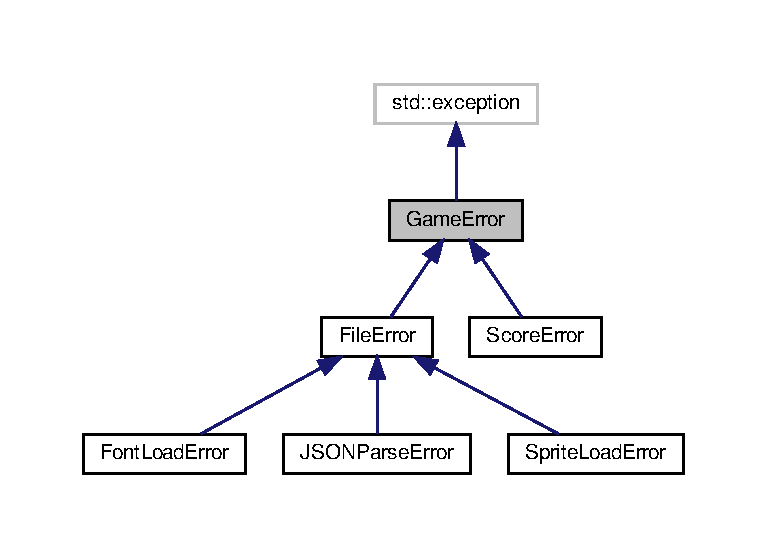
\includegraphics[width=350pt]{classGameError__inherit__graph}
\end{center}
\end{figure}


Collaboration diagram for Game\+Error\+:\nopagebreak
\begin{figure}[H]
\begin{center}
\leavevmode
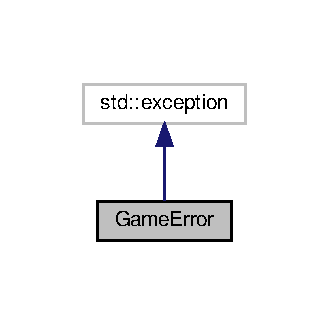
\includegraphics[width=158pt]{classGameError__coll__graph}
\end{center}
\end{figure}
\subsection*{Public Member Functions}
\begin{DoxyCompactItemize}
\item 
virtual const char $\ast$ \hyperlink{classGameError_afbe93d6a2023f2824be2733aff9e86cb}{what} () const noexcept=0
\end{DoxyCompactItemize}


\subsection{Detailed Description}
Base exception class for errors in the game 

\subsection{Member Function Documentation}
\mbox{\Hypertarget{classGameError_afbe93d6a2023f2824be2733aff9e86cb}\label{classGameError_afbe93d6a2023f2824be2733aff9e86cb}} 
\index{Game\+Error@{Game\+Error}!what@{what}}
\index{what@{what}!Game\+Error@{Game\+Error}}
\subsubsection{\texorpdfstring{what()}{what()}}
{\footnotesize\ttfamily virtual const char$\ast$ Game\+Error\+::what (\begin{DoxyParamCaption}{ }\end{DoxyParamCaption}) const\hspace{0.3cm}{\ttfamily [pure virtual]}, {\ttfamily [noexcept]}}

Return the error message \begin{DoxyReturn}{Returns}

\end{DoxyReturn}


Implemented in \hyperlink{classSpriteLoadError_a7b51c2ea656c91b352514cd77aab0a38}{Sprite\+Load\+Error}, \hyperlink{classJSONParseError_a1f33b495974db21a050ede28eb0fe298}{J\+S\+O\+N\+Parse\+Error}, \hyperlink{classFontLoadError_a523f16150eb19d25ed5692512e6952f5}{Font\+Load\+Error}, and \hyperlink{classScoreError_a56e2018c9c0c9d34b482533aa983d37d}{Score\+Error}.



The documentation for this class was generated from the following file\+:\begin{DoxyCompactItemize}
\item 
Exception\+\_\+class/Game\+Error.\+h\end{DoxyCompactItemize}

\hypertarget{classJSONParseError}{}\section{J\+S\+O\+N\+Parse\+Error Class Reference}
\label{classJSONParseError}\index{J\+S\+O\+N\+Parse\+Error@{J\+S\+O\+N\+Parse\+Error}}


{\ttfamily \#include $<$J\+S\+O\+N\+Parse\+Error.\+h$>$}



Inheritance diagram for J\+S\+O\+N\+Parse\+Error\+:\nopagebreak
\begin{figure}[H]
\begin{center}
\leavevmode
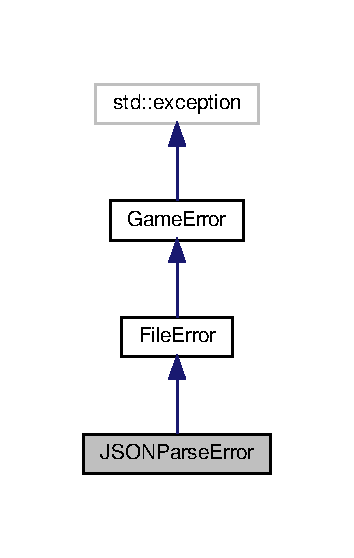
\includegraphics[width=170pt]{classJSONParseError__inherit__graph}
\end{center}
\end{figure}


Collaboration diagram for J\+S\+O\+N\+Parse\+Error\+:\nopagebreak
\begin{figure}[H]
\begin{center}
\leavevmode
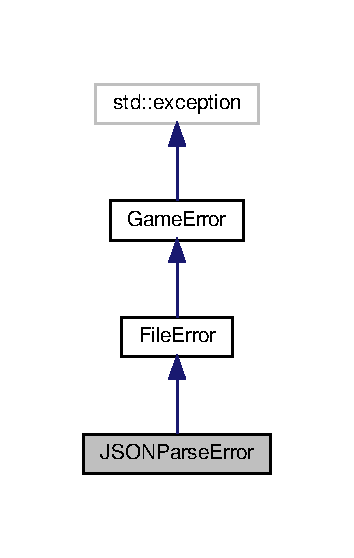
\includegraphics[width=170pt]{classJSONParseError__coll__graph}
\end{center}
\end{figure}
\subsection*{Public Member Functions}
\begin{DoxyCompactItemize}
\item 
\hyperlink{classJSONParseError_a92ab01ff5045faea98f10ed307b6306d}{J\+S\+O\+N\+Parse\+Error} (const char $\ast$\hyperlink{classFileError_a0ea1cc225bf7f8fa47aa0cfa0c2ba685}{file})
\item 
const char $\ast$ \hyperlink{classJSONParseError_a1f33b495974db21a050ede28eb0fe298}{what} () const noexcept override
\item 
const char $\ast$ \hyperlink{classJSONParseError_a24c5c1358b6ae6c96b30ebaa96e0a30b}{file\+Path} () const noexcept override
\end{DoxyCompactItemize}
\subsection*{Additional Inherited Members}


\subsection{Detailed Description}
Error that appears when there is a mistake while parsing or loading a json file 

\subsection{Constructor \& Destructor Documentation}
\mbox{\Hypertarget{classJSONParseError_a92ab01ff5045faea98f10ed307b6306d}\label{classJSONParseError_a92ab01ff5045faea98f10ed307b6306d}} 
\index{J\+S\+O\+N\+Parse\+Error@{J\+S\+O\+N\+Parse\+Error}!J\+S\+O\+N\+Parse\+Error@{J\+S\+O\+N\+Parse\+Error}}
\index{J\+S\+O\+N\+Parse\+Error@{J\+S\+O\+N\+Parse\+Error}!J\+S\+O\+N\+Parse\+Error@{J\+S\+O\+N\+Parse\+Error}}
\subsubsection{\texorpdfstring{J\+S\+O\+N\+Parse\+Error()}{JSONParseError()}}
{\footnotesize\ttfamily J\+S\+O\+N\+Parse\+Error\+::\+J\+S\+O\+N\+Parse\+Error (\begin{DoxyParamCaption}\item[{const char $\ast$}]{file }\end{DoxyParamCaption})}

Constructor with file that contained the error 
\begin{DoxyParams}{Parameters}
{\em file} & \\
\hline
\end{DoxyParams}


\subsection{Member Function Documentation}
\mbox{\Hypertarget{classJSONParseError_a24c5c1358b6ae6c96b30ebaa96e0a30b}\label{classJSONParseError_a24c5c1358b6ae6c96b30ebaa96e0a30b}} 
\index{J\+S\+O\+N\+Parse\+Error@{J\+S\+O\+N\+Parse\+Error}!file\+Path@{file\+Path}}
\index{file\+Path@{file\+Path}!J\+S\+O\+N\+Parse\+Error@{J\+S\+O\+N\+Parse\+Error}}
\subsubsection{\texorpdfstring{file\+Path()}{filePath()}}
{\footnotesize\ttfamily const char $\ast$ J\+S\+O\+N\+Parse\+Error\+::file\+Path (\begin{DoxyParamCaption}{ }\end{DoxyParamCaption}) const\hspace{0.3cm}{\ttfamily [override]}, {\ttfamily [virtual]}, {\ttfamily [noexcept]}}

Returns the file that caused the erro \begin{DoxyReturn}{Returns}

\end{DoxyReturn}


Implements \hyperlink{classFileError_a40918f5dda2ee7063bba81d286392cdd}{File\+Error}.

\mbox{\Hypertarget{classJSONParseError_a1f33b495974db21a050ede28eb0fe298}\label{classJSONParseError_a1f33b495974db21a050ede28eb0fe298}} 
\index{J\+S\+O\+N\+Parse\+Error@{J\+S\+O\+N\+Parse\+Error}!what@{what}}
\index{what@{what}!J\+S\+O\+N\+Parse\+Error@{J\+S\+O\+N\+Parse\+Error}}
\subsubsection{\texorpdfstring{what()}{what()}}
{\footnotesize\ttfamily const char $\ast$ J\+S\+O\+N\+Parse\+Error\+::what (\begin{DoxyParamCaption}{ }\end{DoxyParamCaption}) const\hspace{0.3cm}{\ttfamily [override]}, {\ttfamily [virtual]}, {\ttfamily [noexcept]}}

Returns the error message \begin{DoxyReturn}{Returns}

\end{DoxyReturn}


Implements \hyperlink{classGameError_afbe93d6a2023f2824be2733aff9e86cb}{Game\+Error}.



The documentation for this class was generated from the following files\+:\begin{DoxyCompactItemize}
\item 
Exception\+\_\+class/J\+S\+O\+N\+Parse\+Error.\+h\item 
Exception\+\_\+class/J\+S\+O\+N\+Parse\+Error.\+cpp\end{DoxyCompactItemize}

\hypertarget{classMenu}{}\section{Menu Class Reference}
\label{classMenu}\index{Menu@{Menu}}


{\ttfamily \#include $<$Menu.\+h$>$}

\subsection*{Public Member Functions}
\begin{DoxyCompactItemize}
\item 
\hyperlink{classMenu_a059f49ef452f21afc977008f58117aeb}{Menu} (std\+::shared\+\_\+ptr$<$ sf\+::\+Render\+Window $>$ window, std\+::shared\+\_\+ptr$<$ \hyperlink{classConfigData}{Config\+Data} $>$ config)
\item 
void \hyperlink{classMenu_a9df102abcebc51e69c4728dc3d3c3be0}{draw\+Menu} ()
\item 
void \hyperlink{classMenu_a7477c08823e9322963d9cac0b326d87f}{Up} ()
\item 
void \hyperlink{classMenu_a2963765d4666e9f4dea6b3e508a020a9}{Down} ()
\item 
int \hyperlink{classMenu_a30033d60fd0e4dedc92fb298ecfda7f8}{Get\+Selected} ()
\end{DoxyCompactItemize}


\subsection{Detailed Description}
\hyperlink{classMenu}{Menu} class, handles the game menu and the level select 

\subsection{Constructor \& Destructor Documentation}
\mbox{\Hypertarget{classMenu_a059f49ef452f21afc977008f58117aeb}\label{classMenu_a059f49ef452f21afc977008f58117aeb}} 
\index{Menu@{Menu}!Menu@{Menu}}
\index{Menu@{Menu}!Menu@{Menu}}
\subsubsection{\texorpdfstring{Menu()}{Menu()}}
{\footnotesize\ttfamily Menu\+::\+Menu (\begin{DoxyParamCaption}\item[{std\+::shared\+\_\+ptr$<$ sf\+::\+Render\+Window $>$}]{window,  }\item[{std\+::shared\+\_\+ptr$<$ \hyperlink{classConfigData}{Config\+Data} $>$}]{config }\end{DoxyParamCaption})}

Constructor with sfml window and configuration data 
\begin{DoxyParams}{Parameters}
{\em window} & \\
\hline
{\em config} & \\
\hline
\end{DoxyParams}


\subsection{Member Function Documentation}
\mbox{\Hypertarget{classMenu_a2963765d4666e9f4dea6b3e508a020a9}\label{classMenu_a2963765d4666e9f4dea6b3e508a020a9}} 
\index{Menu@{Menu}!Down@{Down}}
\index{Down@{Down}!Menu@{Menu}}
\subsubsection{\texorpdfstring{Down()}{Down()}}
{\footnotesize\ttfamily void Menu\+::\+Down (\begin{DoxyParamCaption}{ }\end{DoxyParamCaption})}

Move down \mbox{\Hypertarget{classMenu_a9df102abcebc51e69c4728dc3d3c3be0}\label{classMenu_a9df102abcebc51e69c4728dc3d3c3be0}} 
\index{Menu@{Menu}!draw\+Menu@{draw\+Menu}}
\index{draw\+Menu@{draw\+Menu}!Menu@{Menu}}
\subsubsection{\texorpdfstring{draw\+Menu()}{drawMenu()}}
{\footnotesize\ttfamily void Menu\+::draw\+Menu (\begin{DoxyParamCaption}{ }\end{DoxyParamCaption})}

Draw the menu \mbox{\Hypertarget{classMenu_a30033d60fd0e4dedc92fb298ecfda7f8}\label{classMenu_a30033d60fd0e4dedc92fb298ecfda7f8}} 
\index{Menu@{Menu}!Get\+Selected@{Get\+Selected}}
\index{Get\+Selected@{Get\+Selected}!Menu@{Menu}}
\subsubsection{\texorpdfstring{Get\+Selected()}{GetSelected()}}
{\footnotesize\ttfamily int Menu\+::\+Get\+Selected (\begin{DoxyParamCaption}{ }\end{DoxyParamCaption})}

Give back the selected item \begin{DoxyReturn}{Returns}
integer 
\end{DoxyReturn}
\mbox{\Hypertarget{classMenu_a7477c08823e9322963d9cac0b326d87f}\label{classMenu_a7477c08823e9322963d9cac0b326d87f}} 
\index{Menu@{Menu}!Up@{Up}}
\index{Up@{Up}!Menu@{Menu}}
\subsubsection{\texorpdfstring{Up()}{Up()}}
{\footnotesize\ttfamily void Menu\+::\+Up (\begin{DoxyParamCaption}{ }\end{DoxyParamCaption})}

Move up 

The documentation for this class was generated from the following files\+:\begin{DoxyCompactItemize}
\item 
Menu.\+h\item 
Menu.\+cpp\end{DoxyCompactItemize}

\hypertarget{classroadfighter_1_1MovingCar}{}\section{roadfighter\+:\+:Moving\+Car Class Reference}
\label{classroadfighter_1_1MovingCar}\index{roadfighter\+::\+Moving\+Car@{roadfighter\+::\+Moving\+Car}}


{\ttfamily \#include $<$Moving\+Car.\+h$>$}



Inheritance diagram for roadfighter\+:\+:Moving\+Car\+:\nopagebreak
\begin{figure}[H]
\begin{center}
\leavevmode
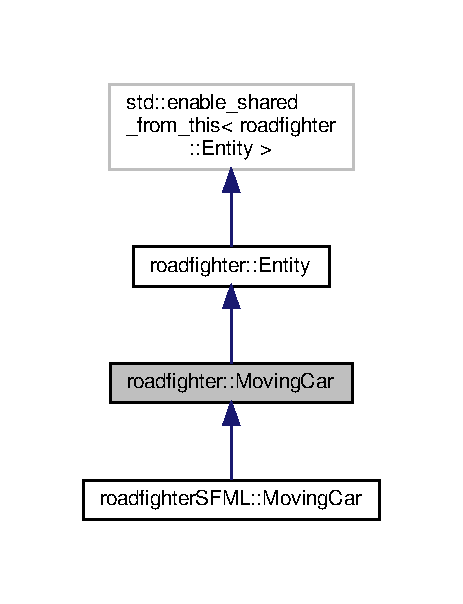
\includegraphics[width=222pt]{classroadfighter_1_1MovingCar__inherit__graph}
\end{center}
\end{figure}


Collaboration diagram for roadfighter\+:\+:Moving\+Car\+:\nopagebreak
\begin{figure}[H]
\begin{center}
\leavevmode
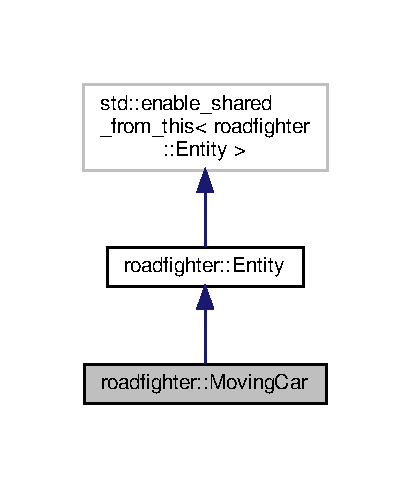
\includegraphics[width=197pt]{classroadfighter_1_1MovingCar__coll__graph}
\end{center}
\end{figure}
\subsection*{Public Member Functions}
\begin{DoxyCompactItemize}
\item 
\hyperlink{classroadfighter_1_1MovingCar_a938e531ba0de68f564f188d55a59e138}{Moving\+Car} (std\+::shared\+\_\+ptr$<$ \hyperlink{classConfigData}{Config\+Data} $>$ config)
\item 
void \hyperlink{classroadfighter_1_1MovingCar_a06c6e2e0510707bdd7e4570b8f65241c}{update} () override
\item 
void \hyperlink{classroadfighter_1_1MovingCar_a62fbe61c5a1c1a1c0d376047ec1edcf2}{update} (int \hyperlink{classroadfighter_1_1MovingCar_aa11ffbdab47c7fdf1311cfe02f0d8bd7}{speed}, std\+::shared\+\_\+ptr$<$ \hyperlink{classroadfighter_1_1Entity}{roadfighter\+::\+Entity} $>$ Player) override
\item 
int \hyperlink{classroadfighter_1_1MovingCar_a42bdd9382e7234ae79d6f5e582adee92}{get\+Speed} () override
\item 
int \hyperlink{classroadfighter_1_1MovingCar_a97196aa72de773ac88d1df99c47a5367}{Delete} () override
\item 
std\+::shared\+\_\+ptr$<$ \hyperlink{structObjBox}{Obj\+Box} $>$ \hyperlink{classroadfighter_1_1MovingCar_a8b744958eaba45078e98fad4ac6821c3}{get\+Objbox} () override
\item 
void \hyperlink{classroadfighter_1_1MovingCar_a2fd9123a7ee59d4796672ad79656e1b5}{set\+Delete} (int del) override
\item 
bool \hyperlink{classroadfighter_1_1MovingCar_a5b7a6cf114fe26016434b2fcf3434d37}{Shoot} () override
\end{DoxyCompactItemize}
\subsection*{Protected Attributes}
\begin{DoxyCompactItemize}
\item 
std\+::pair$<$ double, double $>$ \hyperlink{classroadfighter_1_1MovingCar_abff584d4890e348c74f3ac3962d2df9c}{centralpos}
\item 
int \hyperlink{classroadfighter_1_1MovingCar_aa11ffbdab47c7fdf1311cfe02f0d8bd7}{speed}
\item 
int \hyperlink{classroadfighter_1_1MovingCar_a326ee7c0301dd03d570d3820612614ca}{to\+Del} = 0
\item 
double \hyperlink{classroadfighter_1_1MovingCar_aa8068e11ad7fa9311c0703b306119f53}{height}
\item 
double \hyperlink{classroadfighter_1_1MovingCar_af13dfca7a365dd785dbfc2c8446232a9}{width}
\item 
double \hyperlink{classroadfighter_1_1MovingCar_a60a80bd76b33c59a836a57606a19d7e6}{moves\+Left} = 0.\+6
\end{DoxyCompactItemize}


\subsection{Detailed Description}
The Moving car that moves to the player when it passes the player 

\subsection{Constructor \& Destructor Documentation}
\mbox{\Hypertarget{classroadfighter_1_1MovingCar_a938e531ba0de68f564f188d55a59e138}\label{classroadfighter_1_1MovingCar_a938e531ba0de68f564f188d55a59e138}} 
\index{roadfighter\+::\+Moving\+Car@{roadfighter\+::\+Moving\+Car}!Moving\+Car@{Moving\+Car}}
\index{Moving\+Car@{Moving\+Car}!roadfighter\+::\+Moving\+Car@{roadfighter\+::\+Moving\+Car}}
\subsubsection{\texorpdfstring{Moving\+Car()}{MovingCar()}}
{\footnotesize\ttfamily roadfighter\+::\+Moving\+Car\+::\+Moving\+Car (\begin{DoxyParamCaption}\item[{std\+::shared\+\_\+ptr$<$ \hyperlink{classConfigData}{Config\+Data} $>$}]{config }\end{DoxyParamCaption})}

Constructor with the configuration data 
\begin{DoxyParams}{Parameters}
{\em config} & \\
\hline
\end{DoxyParams}


\subsection{Member Function Documentation}
\mbox{\Hypertarget{classroadfighter_1_1MovingCar_a97196aa72de773ac88d1df99c47a5367}\label{classroadfighter_1_1MovingCar_a97196aa72de773ac88d1df99c47a5367}} 
\index{roadfighter\+::\+Moving\+Car@{roadfighter\+::\+Moving\+Car}!Delete@{Delete}}
\index{Delete@{Delete}!roadfighter\+::\+Moving\+Car@{roadfighter\+::\+Moving\+Car}}
\subsubsection{\texorpdfstring{Delete()}{Delete()}}
{\footnotesize\ttfamily int roadfighter\+::\+Moving\+Car\+::\+Delete (\begin{DoxyParamCaption}{ }\end{DoxyParamCaption})\hspace{0.3cm}{\ttfamily [override]}, {\ttfamily [virtual]}}

Returns a certain value to determine the delete status 0 = nothing, 1 = delete, 2 = respawn \begin{DoxyReturn}{Returns}

\end{DoxyReturn}


Implements \hyperlink{classroadfighter_1_1Entity_a08190b0b8e6a3fcdb42273d6096152ac}{roadfighter\+::\+Entity}.

\mbox{\Hypertarget{classroadfighter_1_1MovingCar_a8b744958eaba45078e98fad4ac6821c3}\label{classroadfighter_1_1MovingCar_a8b744958eaba45078e98fad4ac6821c3}} 
\index{roadfighter\+::\+Moving\+Car@{roadfighter\+::\+Moving\+Car}!get\+Objbox@{get\+Objbox}}
\index{get\+Objbox@{get\+Objbox}!roadfighter\+::\+Moving\+Car@{roadfighter\+::\+Moving\+Car}}
\subsubsection{\texorpdfstring{get\+Objbox()}{getObjbox()}}
{\footnotesize\ttfamily std\+::shared\+\_\+ptr$<$ \hyperlink{structObjBox}{Obj\+Box} $>$ roadfighter\+::\+Moving\+Car\+::get\+Objbox (\begin{DoxyParamCaption}{ }\end{DoxyParamCaption})\hspace{0.3cm}{\ttfamily [override]}, {\ttfamily [virtual]}}

Return a shared\+\_\+ptr of the object box \begin{DoxyReturn}{Returns}

\end{DoxyReturn}


Implements \hyperlink{classroadfighter_1_1Entity_af14340d04a725175a6d221f23c35fa0c}{roadfighter\+::\+Entity}.

\mbox{\Hypertarget{classroadfighter_1_1MovingCar_a42bdd9382e7234ae79d6f5e582adee92}\label{classroadfighter_1_1MovingCar_a42bdd9382e7234ae79d6f5e582adee92}} 
\index{roadfighter\+::\+Moving\+Car@{roadfighter\+::\+Moving\+Car}!get\+Speed@{get\+Speed}}
\index{get\+Speed@{get\+Speed}!roadfighter\+::\+Moving\+Car@{roadfighter\+::\+Moving\+Car}}
\subsubsection{\texorpdfstring{get\+Speed()}{getSpeed()}}
{\footnotesize\ttfamily int roadfighter\+::\+Moving\+Car\+::get\+Speed (\begin{DoxyParamCaption}{ }\end{DoxyParamCaption})\hspace{0.3cm}{\ttfamily [override]}, {\ttfamily [virtual]}}

Returns the speed of the object \begin{DoxyReturn}{Returns}
speed 
\end{DoxyReturn}


Implements \hyperlink{classroadfighter_1_1Entity_ad3760184d764a61922e1db7d98501ee4}{roadfighter\+::\+Entity}.

\mbox{\Hypertarget{classroadfighter_1_1MovingCar_a2fd9123a7ee59d4796672ad79656e1b5}\label{classroadfighter_1_1MovingCar_a2fd9123a7ee59d4796672ad79656e1b5}} 
\index{roadfighter\+::\+Moving\+Car@{roadfighter\+::\+Moving\+Car}!set\+Delete@{set\+Delete}}
\index{set\+Delete@{set\+Delete}!roadfighter\+::\+Moving\+Car@{roadfighter\+::\+Moving\+Car}}
\subsubsection{\texorpdfstring{set\+Delete()}{setDelete()}}
{\footnotesize\ttfamily void roadfighter\+::\+Moving\+Car\+::set\+Delete (\begin{DoxyParamCaption}\item[{int}]{del }\end{DoxyParamCaption})\hspace{0.3cm}{\ttfamily [override]}, {\ttfamily [virtual]}}

Set if an object must be deleted or not 
\begin{DoxyParams}{Parameters}
{\em del} & \\
\hline
\end{DoxyParams}


Implements \hyperlink{classroadfighter_1_1Entity_a07e973f0fa941a69e749629716877692}{roadfighter\+::\+Entity}.

\mbox{\Hypertarget{classroadfighter_1_1MovingCar_a5b7a6cf114fe26016434b2fcf3434d37}\label{classroadfighter_1_1MovingCar_a5b7a6cf114fe26016434b2fcf3434d37}} 
\index{roadfighter\+::\+Moving\+Car@{roadfighter\+::\+Moving\+Car}!Shoot@{Shoot}}
\index{Shoot@{Shoot}!roadfighter\+::\+Moving\+Car@{roadfighter\+::\+Moving\+Car}}
\subsubsection{\texorpdfstring{Shoot()}{Shoot()}}
{\footnotesize\ttfamily bool roadfighter\+::\+Moving\+Car\+::\+Shoot (\begin{DoxyParamCaption}{ }\end{DoxyParamCaption})\hspace{0.3cm}{\ttfamily [override]}, {\ttfamily [virtual]}}

Return if the object shot \begin{DoxyReturn}{Returns}

\end{DoxyReturn}


Implements \hyperlink{classroadfighter_1_1Entity_ad0ecaa0539db252e591da83814251509}{roadfighter\+::\+Entity}.

\mbox{\Hypertarget{classroadfighter_1_1MovingCar_a06c6e2e0510707bdd7e4570b8f65241c}\label{classroadfighter_1_1MovingCar_a06c6e2e0510707bdd7e4570b8f65241c}} 
\index{roadfighter\+::\+Moving\+Car@{roadfighter\+::\+Moving\+Car}!update@{update}}
\index{update@{update}!roadfighter\+::\+Moving\+Car@{roadfighter\+::\+Moving\+Car}}
\subsubsection{\texorpdfstring{update()}{update()}\hspace{0.1cm}{\footnotesize\ttfamily [1/2]}}
{\footnotesize\ttfamily void roadfighter\+::\+Moving\+Car\+::update (\begin{DoxyParamCaption}{ }\end{DoxyParamCaption})\hspace{0.3cm}{\ttfamily [override]}, {\ttfamily [virtual]}}

Update 

Implements \hyperlink{classroadfighter_1_1Entity_a19cd353f12a3e8432acd6d5609137561}{roadfighter\+::\+Entity}.

\mbox{\Hypertarget{classroadfighter_1_1MovingCar_a62fbe61c5a1c1a1c0d376047ec1edcf2}\label{classroadfighter_1_1MovingCar_a62fbe61c5a1c1a1c0d376047ec1edcf2}} 
\index{roadfighter\+::\+Moving\+Car@{roadfighter\+::\+Moving\+Car}!update@{update}}
\index{update@{update}!roadfighter\+::\+Moving\+Car@{roadfighter\+::\+Moving\+Car}}
\subsubsection{\texorpdfstring{update()}{update()}\hspace{0.1cm}{\footnotesize\ttfamily [2/2]}}
{\footnotesize\ttfamily void roadfighter\+::\+Moving\+Car\+::update (\begin{DoxyParamCaption}\item[{int}]{speed,  }\item[{std\+::shared\+\_\+ptr$<$ \hyperlink{classroadfighter_1_1Entity}{roadfighter\+::\+Entity} $>$}]{Player }\end{DoxyParamCaption})\hspace{0.3cm}{\ttfamily [override]}, {\ttfamily [virtual]}}

Updates the object with extra parameters 
\begin{DoxyParams}{Parameters}
{\em speed} & \\
\hline
{\em Player} & \\
\hline
\end{DoxyParams}


Implements \hyperlink{classroadfighter_1_1Entity_a611ba56595dd2137d308876ba820cc09}{roadfighter\+::\+Entity}.



\subsection{Member Data Documentation}
\mbox{\Hypertarget{classroadfighter_1_1MovingCar_abff584d4890e348c74f3ac3962d2df9c}\label{classroadfighter_1_1MovingCar_abff584d4890e348c74f3ac3962d2df9c}} 
\index{roadfighter\+::\+Moving\+Car@{roadfighter\+::\+Moving\+Car}!centralpos@{centralpos}}
\index{centralpos@{centralpos}!roadfighter\+::\+Moving\+Car@{roadfighter\+::\+Moving\+Car}}
\subsubsection{\texorpdfstring{centralpos}{centralpos}}
{\footnotesize\ttfamily std\+::pair$<$double, double$>$ roadfighter\+::\+Moving\+Car\+::centralpos\hspace{0.3cm}{\ttfamily [protected]}}

Pair of the doubles that contains the x and y position of the center of the object \mbox{\Hypertarget{classroadfighter_1_1MovingCar_aa8068e11ad7fa9311c0703b306119f53}\label{classroadfighter_1_1MovingCar_aa8068e11ad7fa9311c0703b306119f53}} 
\index{roadfighter\+::\+Moving\+Car@{roadfighter\+::\+Moving\+Car}!height@{height}}
\index{height@{height}!roadfighter\+::\+Moving\+Car@{roadfighter\+::\+Moving\+Car}}
\subsubsection{\texorpdfstring{height}{height}}
{\footnotesize\ttfamily double roadfighter\+::\+Moving\+Car\+::height\hspace{0.3cm}{\ttfamily [protected]}}

Height of the object \mbox{\Hypertarget{classroadfighter_1_1MovingCar_a60a80bd76b33c59a836a57606a19d7e6}\label{classroadfighter_1_1MovingCar_a60a80bd76b33c59a836a57606a19d7e6}} 
\index{roadfighter\+::\+Moving\+Car@{roadfighter\+::\+Moving\+Car}!moves\+Left@{moves\+Left}}
\index{moves\+Left@{moves\+Left}!roadfighter\+::\+Moving\+Car@{roadfighter\+::\+Moving\+Car}}
\subsubsection{\texorpdfstring{moves\+Left}{movesLeft}}
{\footnotesize\ttfamily double roadfighter\+::\+Moving\+Car\+::moves\+Left = 0.\+6\hspace{0.3cm}{\ttfamily [protected]}}

Distance the car is allowed to move left or right \mbox{\Hypertarget{classroadfighter_1_1MovingCar_aa11ffbdab47c7fdf1311cfe02f0d8bd7}\label{classroadfighter_1_1MovingCar_aa11ffbdab47c7fdf1311cfe02f0d8bd7}} 
\index{roadfighter\+::\+Moving\+Car@{roadfighter\+::\+Moving\+Car}!speed@{speed}}
\index{speed@{speed}!roadfighter\+::\+Moving\+Car@{roadfighter\+::\+Moving\+Car}}
\subsubsection{\texorpdfstring{speed}{speed}}
{\footnotesize\ttfamily int roadfighter\+::\+Moving\+Car\+::speed\hspace{0.3cm}{\ttfamily [protected]}}

Speed of the object \mbox{\Hypertarget{classroadfighter_1_1MovingCar_a326ee7c0301dd03d570d3820612614ca}\label{classroadfighter_1_1MovingCar_a326ee7c0301dd03d570d3820612614ca}} 
\index{roadfighter\+::\+Moving\+Car@{roadfighter\+::\+Moving\+Car}!to\+Del@{to\+Del}}
\index{to\+Del@{to\+Del}!roadfighter\+::\+Moving\+Car@{roadfighter\+::\+Moving\+Car}}
\subsubsection{\texorpdfstring{to\+Del}{toDel}}
{\footnotesize\ttfamily int roadfighter\+::\+Moving\+Car\+::to\+Del = 0\hspace{0.3cm}{\ttfamily [protected]}}

Object deletion status ( 0 = nothing, 1 = delete, 2 = respawn ) \mbox{\Hypertarget{classroadfighter_1_1MovingCar_af13dfca7a365dd785dbfc2c8446232a9}\label{classroadfighter_1_1MovingCar_af13dfca7a365dd785dbfc2c8446232a9}} 
\index{roadfighter\+::\+Moving\+Car@{roadfighter\+::\+Moving\+Car}!width@{width}}
\index{width@{width}!roadfighter\+::\+Moving\+Car@{roadfighter\+::\+Moving\+Car}}
\subsubsection{\texorpdfstring{width}{width}}
{\footnotesize\ttfamily double roadfighter\+::\+Moving\+Car\+::width\hspace{0.3cm}{\ttfamily [protected]}}

Width of the object 

The documentation for this class was generated from the following files\+:\begin{DoxyCompactItemize}
\item 
roadfighter/Moving\+Car.\+h\item 
roadfighter/Moving\+Car.\+cpp\end{DoxyCompactItemize}

\hypertarget{classroadfighterSFML_1_1MovingCar}{}\section{roadfighter\+S\+F\+ML\+:\+:Moving\+Car Class Reference}
\label{classroadfighterSFML_1_1MovingCar}\index{roadfighter\+S\+F\+M\+L\+::\+Moving\+Car@{roadfighter\+S\+F\+M\+L\+::\+Moving\+Car}}


{\ttfamily \#include $<$Moving\+Car.\+h$>$}



Inheritance diagram for roadfighter\+S\+F\+ML\+:\+:Moving\+Car\+:\nopagebreak
\begin{figure}[H]
\begin{center}
\leavevmode
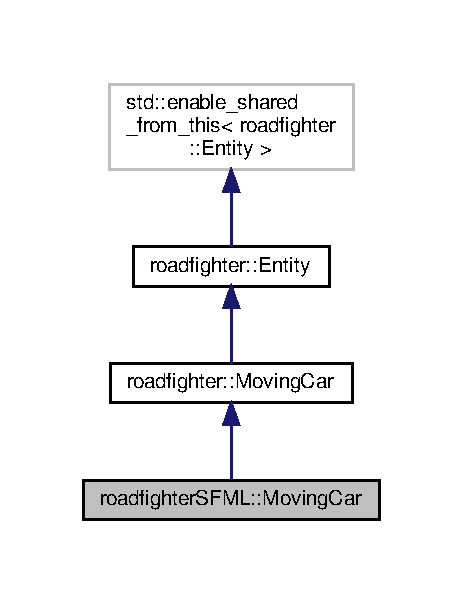
\includegraphics[width=222pt]{classroadfighterSFML_1_1MovingCar__inherit__graph}
\end{center}
\end{figure}


Collaboration diagram for roadfighter\+S\+F\+ML\+:\+:Moving\+Car\+:\nopagebreak
\begin{figure}[H]
\begin{center}
\leavevmode
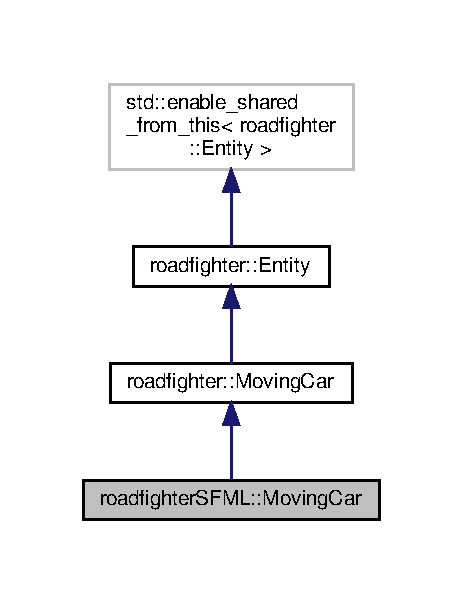
\includegraphics[width=222pt]{classroadfighterSFML_1_1MovingCar__coll__graph}
\end{center}
\end{figure}
\subsection*{Public Member Functions}
\begin{DoxyCompactItemize}
\item 
\hyperlink{classroadfighterSFML_1_1MovingCar_a65f36a04c68c9c4756616aabbc029b27}{Moving\+Car} (const std\+::shared\+\_\+ptr$<$ sf\+::\+Render\+Window $>$ window, double random, std\+::shared\+\_\+ptr$<$ \hyperlink{classConfigData}{Config\+Data} $>$ config)
\item 
void \hyperlink{classroadfighterSFML_1_1MovingCar_afff9b85787e5af092cce59be3370a683}{draw} () override
\end{DoxyCompactItemize}
\subsection*{Additional Inherited Members}


\subsection{Detailed Description}
Graphic side of movingcar 

\subsection{Constructor \& Destructor Documentation}
\mbox{\Hypertarget{classroadfighterSFML_1_1MovingCar_a65f36a04c68c9c4756616aabbc029b27}\label{classroadfighterSFML_1_1MovingCar_a65f36a04c68c9c4756616aabbc029b27}} 
\index{roadfighter\+S\+F\+M\+L\+::\+Moving\+Car@{roadfighter\+S\+F\+M\+L\+::\+Moving\+Car}!Moving\+Car@{Moving\+Car}}
\index{Moving\+Car@{Moving\+Car}!roadfighter\+S\+F\+M\+L\+::\+Moving\+Car@{roadfighter\+S\+F\+M\+L\+::\+Moving\+Car}}
\subsubsection{\texorpdfstring{Moving\+Car()}{MovingCar()}}
{\footnotesize\ttfamily roadfighter\+S\+F\+M\+L\+::\+Moving\+Car\+::\+Moving\+Car (\begin{DoxyParamCaption}\item[{const std\+::shared\+\_\+ptr$<$ sf\+::\+Render\+Window $>$}]{window,  }\item[{double}]{random,  }\item[{std\+::shared\+\_\+ptr$<$ \hyperlink{classConfigData}{Config\+Data} $>$}]{config }\end{DoxyParamCaption})}

Constructor with window and a random value to determine the spawning location and configuration data 
\begin{DoxyParams}{Parameters}
{\em window} & \\
\hline
{\em random} & \\
\hline
{\em config} & \\
\hline
\end{DoxyParams}


\subsection{Member Function Documentation}
\mbox{\Hypertarget{classroadfighterSFML_1_1MovingCar_afff9b85787e5af092cce59be3370a683}\label{classroadfighterSFML_1_1MovingCar_afff9b85787e5af092cce59be3370a683}} 
\index{roadfighter\+S\+F\+M\+L\+::\+Moving\+Car@{roadfighter\+S\+F\+M\+L\+::\+Moving\+Car}!draw@{draw}}
\index{draw@{draw}!roadfighter\+S\+F\+M\+L\+::\+Moving\+Car@{roadfighter\+S\+F\+M\+L\+::\+Moving\+Car}}
\subsubsection{\texorpdfstring{draw()}{draw()}}
{\footnotesize\ttfamily void roadfighter\+S\+F\+M\+L\+::\+Moving\+Car\+::draw (\begin{DoxyParamCaption}{ }\end{DoxyParamCaption})\hspace{0.3cm}{\ttfamily [override]}, {\ttfamily [virtual]}}

draws the object 

Implements \hyperlink{classroadfighter_1_1Entity_ac516f8005f969ad5a86c252e5a3640ee}{roadfighter\+::\+Entity}.



The documentation for this class was generated from the following files\+:\begin{DoxyCompactItemize}
\item 
roadfighter\+S\+F\+M\+L/Moving\+Car.\+h\item 
roadfighter\+S\+F\+M\+L/Moving\+Car.\+cpp\end{DoxyCompactItemize}

\hypertarget{structObjBox}{}\section{Obj\+Box Struct Reference}
\label{structObjBox}\index{Obj\+Box@{Obj\+Box}}


{\ttfamily \#include $<$Utils.\+h$>$}

\subsection*{Public Member Functions}
\begin{DoxyCompactItemize}
\item 
\hyperlink{structObjBox_ae82c9aa8ac2715dc917bfa67eb57eb26}{Obj\+Box} (const std\+::pair$<$ float, float $>$ \&\hyperlink{structObjBox_ab19f0fb6939bdfe0c2100859cf3f63e9}{centralpos}, double \hyperlink{structObjBox_a392ed35e68724580f1f16bb25e73f599}{height}, double \hyperlink{structObjBox_a8fb516e7dc226bee6baf1af53d9376d9}{width})
\end{DoxyCompactItemize}
\subsection*{Public Attributes}
\begin{DoxyCompactItemize}
\item 
std\+::pair$<$ float, float $>$ \hyperlink{structObjBox_ab19f0fb6939bdfe0c2100859cf3f63e9}{centralpos}
\item 
double \hyperlink{structObjBox_a392ed35e68724580f1f16bb25e73f599}{height}
\item 
double \hyperlink{structObjBox_a8fb516e7dc226bee6baf1af53d9376d9}{width}
\end{DoxyCompactItemize}


\subsection{Detailed Description}
Struct for returning collision data 

\subsection{Constructor \& Destructor Documentation}
\mbox{\Hypertarget{structObjBox_ae82c9aa8ac2715dc917bfa67eb57eb26}\label{structObjBox_ae82c9aa8ac2715dc917bfa67eb57eb26}} 
\index{Obj\+Box@{Obj\+Box}!Obj\+Box@{Obj\+Box}}
\index{Obj\+Box@{Obj\+Box}!Obj\+Box@{Obj\+Box}}
\subsubsection{\texorpdfstring{Obj\+Box()}{ObjBox()}}
{\footnotesize\ttfamily Obj\+Box\+::\+Obj\+Box (\begin{DoxyParamCaption}\item[{const std\+::pair$<$ float, float $>$ \&}]{centralpos,  }\item[{double}]{height,  }\item[{double}]{width }\end{DoxyParamCaption})\hspace{0.3cm}{\ttfamily [inline]}}

Constructor 
\begin{DoxyParams}{Parameters}
{\em centralpos} & \\
\hline
{\em height} & \\
\hline
{\em width} & \\
\hline
\end{DoxyParams}


\subsection{Member Data Documentation}
\mbox{\Hypertarget{structObjBox_ab19f0fb6939bdfe0c2100859cf3f63e9}\label{structObjBox_ab19f0fb6939bdfe0c2100859cf3f63e9}} 
\index{Obj\+Box@{Obj\+Box}!centralpos@{centralpos}}
\index{centralpos@{centralpos}!Obj\+Box@{Obj\+Box}}
\subsubsection{\texorpdfstring{centralpos}{centralpos}}
{\footnotesize\ttfamily std\+::pair$<$float,float$>$ Obj\+Box\+::centralpos}

Central position of the object \mbox{\Hypertarget{structObjBox_a392ed35e68724580f1f16bb25e73f599}\label{structObjBox_a392ed35e68724580f1f16bb25e73f599}} 
\index{Obj\+Box@{Obj\+Box}!height@{height}}
\index{height@{height}!Obj\+Box@{Obj\+Box}}
\subsubsection{\texorpdfstring{height}{height}}
{\footnotesize\ttfamily double Obj\+Box\+::height}

Height of the object \mbox{\Hypertarget{structObjBox_a8fb516e7dc226bee6baf1af53d9376d9}\label{structObjBox_a8fb516e7dc226bee6baf1af53d9376d9}} 
\index{Obj\+Box@{Obj\+Box}!width@{width}}
\index{width@{width}!Obj\+Box@{Obj\+Box}}
\subsubsection{\texorpdfstring{width}{width}}
{\footnotesize\ttfamily double Obj\+Box\+::width}

width of the object 

The documentation for this struct was generated from the following file\+:\begin{DoxyCompactItemize}
\item 
Utils/Utils.\+h\end{DoxyCompactItemize}

\hypertarget{classObserver}{}\section{Observer Class Reference}
\label{classObserver}\index{Observer@{Observer}}


{\ttfamily \#include $<$Observer.\+h$>$}



Inheritance diagram for Observer\+:\nopagebreak
\begin{figure}[H]
\begin{center}
\leavevmode
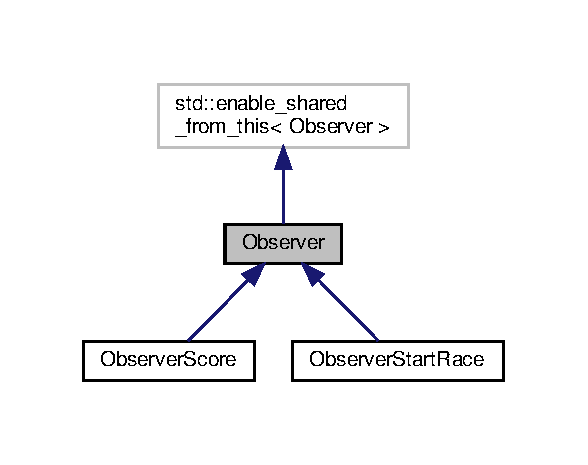
\includegraphics[width=282pt]{classObserver__inherit__graph}
\end{center}
\end{figure}


Collaboration diagram for Observer\+:\nopagebreak
\begin{figure}[H]
\begin{center}
\leavevmode
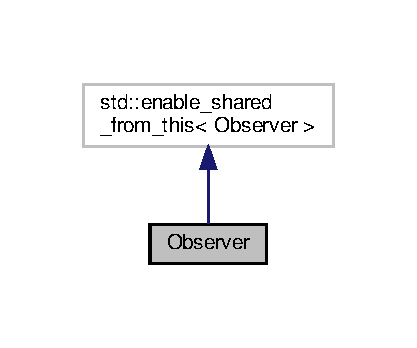
\includegraphics[width=200pt]{classObserver__coll__graph}
\end{center}
\end{figure}
\subsection*{Public Member Functions}
\begin{DoxyCompactItemize}
\item 
\hyperlink{classObserver_a19c43f80a38a332a6f694783df3c9835}{Observer} ()
\item 
virtual void \hyperlink{classObserver_a4b9e6fbc74e7ae6971b2afe462ab5a87}{update} (int score)=0
\item 
virtual std\+::string \hyperlink{classObserver_a92f704d0a3e6e0ade2743da2ae91bcb7}{get\+Type} ()=0
\end{DoxyCompactItemize}


\subsection{Detailed Description}
Base class for the observers 

\subsection{Constructor \& Destructor Documentation}
\mbox{\Hypertarget{classObserver_a19c43f80a38a332a6f694783df3c9835}\label{classObserver_a19c43f80a38a332a6f694783df3c9835}} 
\index{Observer@{Observer}!Observer@{Observer}}
\index{Observer@{Observer}!Observer@{Observer}}
\subsubsection{\texorpdfstring{Observer()}{Observer()}}
{\footnotesize\ttfamily Observer\+::\+Observer (\begin{DoxyParamCaption}{ }\end{DoxyParamCaption})}

Default constructor 

\subsection{Member Function Documentation}
\mbox{\Hypertarget{classObserver_a92f704d0a3e6e0ade2743da2ae91bcb7}\label{classObserver_a92f704d0a3e6e0ade2743da2ae91bcb7}} 
\index{Observer@{Observer}!get\+Type@{get\+Type}}
\index{get\+Type@{get\+Type}!Observer@{Observer}}
\subsubsection{\texorpdfstring{get\+Type()}{getType()}}
{\footnotesize\ttfamily virtual std\+::string Observer\+::get\+Type (\begin{DoxyParamCaption}{ }\end{DoxyParamCaption})\hspace{0.3cm}{\ttfamily [pure virtual]}}

Return the type of the observer \begin{DoxyReturn}{Returns}

\end{DoxyReturn}


Implemented in \hyperlink{classObserverScore_a88ee2b9fe8b49edf234f6c05aa242724}{Observer\+Score}, and \hyperlink{classObserverStartRace_af664693404c9c8f756a8e4ba7d687c3a}{Observer\+Start\+Race}.

\mbox{\Hypertarget{classObserver_a4b9e6fbc74e7ae6971b2afe462ab5a87}\label{classObserver_a4b9e6fbc74e7ae6971b2afe462ab5a87}} 
\index{Observer@{Observer}!update@{update}}
\index{update@{update}!Observer@{Observer}}
\subsubsection{\texorpdfstring{update()}{update()}}
{\footnotesize\ttfamily virtual void Observer\+::update (\begin{DoxyParamCaption}\item[{int}]{score }\end{DoxyParamCaption})\hspace{0.3cm}{\ttfamily [pure virtual]}}

Update with an int parameter 
\begin{DoxyParams}{Parameters}
{\em score} & \\
\hline
\end{DoxyParams}


Implemented in \hyperlink{classObserverScore_a1cb10ae5056c103436e00158cf90d5e4}{Observer\+Score}, and \hyperlink{classObserverStartRace_aa810164d0877c5597ec06adab29b7981}{Observer\+Start\+Race}.



The documentation for this class was generated from the following files\+:\begin{DoxyCompactItemize}
\item 
Observer/Observer.\+h\item 
Observer/Observer.\+cpp\end{DoxyCompactItemize}

\hypertarget{classObserverBackgroundEnd}{}\section{Observer\+Background\+End Class Reference}
\label{classObserverBackgroundEnd}\index{Observer\+Background\+End@{Observer\+Background\+End}}


The documentation for this class was generated from the following file\+:\begin{DoxyCompactItemize}
\item 
Observer/Observer\+Background\+End.\+h\end{DoxyCompactItemize}

\hypertarget{classObserverScore}{}\section{Observer\+Score Class Reference}
\label{classObserverScore}\index{Observer\+Score@{Observer\+Score}}


{\ttfamily \#include $<$Observer\+Score.\+h$>$}



Inheritance diagram for Observer\+Score\+:\nopagebreak
\begin{figure}[H]
\begin{center}
\leavevmode
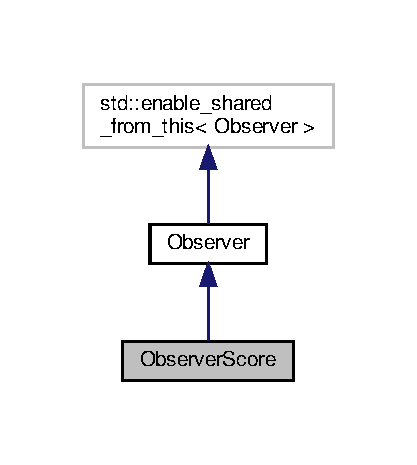
\includegraphics[width=200pt]{classObserverScore__inherit__graph}
\end{center}
\end{figure}


Collaboration diagram for Observer\+Score\+:\nopagebreak
\begin{figure}[H]
\begin{center}
\leavevmode
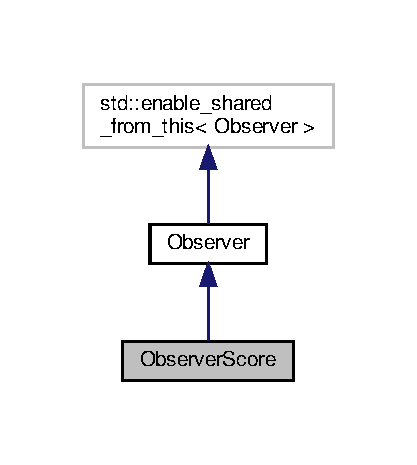
\includegraphics[width=200pt]{classObserverScore__coll__graph}
\end{center}
\end{figure}
\subsection*{Public Member Functions}
\begin{DoxyCompactItemize}
\item 
\hyperlink{classObserverScore_aa0913a7e696f26eb26934bb30a90a6f6}{Observer\+Score} (std\+::shared\+\_\+ptr$<$ sf\+::\+Render\+Window $>$ wind)
\item 
void \hyperlink{classObserverScore_a1cb10ae5056c103436e00158cf90d5e4}{update} (int score) override
\item 
std\+::string \hyperlink{classObserverScore_a88ee2b9fe8b49edf234f6c05aa242724}{get\+Type} () override
\end{DoxyCompactItemize}


\subsection{Detailed Description}
The observer that handles the score 

\subsection{Constructor \& Destructor Documentation}
\mbox{\Hypertarget{classObserverScore_aa0913a7e696f26eb26934bb30a90a6f6}\label{classObserverScore_aa0913a7e696f26eb26934bb30a90a6f6}} 
\index{Observer\+Score@{Observer\+Score}!Observer\+Score@{Observer\+Score}}
\index{Observer\+Score@{Observer\+Score}!Observer\+Score@{Observer\+Score}}
\subsubsection{\texorpdfstring{Observer\+Score()}{ObserverScore()}}
{\footnotesize\ttfamily Observer\+Score\+::\+Observer\+Score (\begin{DoxyParamCaption}\item[{std\+::shared\+\_\+ptr$<$ sf\+::\+Render\+Window $>$}]{wind }\end{DoxyParamCaption})}

Constructor with sfml window 
\begin{DoxyParams}{Parameters}
{\em wind} & \\
\hline
\end{DoxyParams}


\subsection{Member Function Documentation}
\mbox{\Hypertarget{classObserverScore_a88ee2b9fe8b49edf234f6c05aa242724}\label{classObserverScore_a88ee2b9fe8b49edf234f6c05aa242724}} 
\index{Observer\+Score@{Observer\+Score}!get\+Type@{get\+Type}}
\index{get\+Type@{get\+Type}!Observer\+Score@{Observer\+Score}}
\subsubsection{\texorpdfstring{get\+Type()}{getType()}}
{\footnotesize\ttfamily std\+::string Observer\+Score\+::get\+Type (\begin{DoxyParamCaption}{ }\end{DoxyParamCaption})\hspace{0.3cm}{\ttfamily [override]}, {\ttfamily [virtual]}}

Returns the type of the observer \begin{DoxyReturn}{Returns}

\end{DoxyReturn}


Implements \hyperlink{classObserver_a92f704d0a3e6e0ade2743da2ae91bcb7}{Observer}.

\mbox{\Hypertarget{classObserverScore_a1cb10ae5056c103436e00158cf90d5e4}\label{classObserverScore_a1cb10ae5056c103436e00158cf90d5e4}} 
\index{Observer\+Score@{Observer\+Score}!update@{update}}
\index{update@{update}!Observer\+Score@{Observer\+Score}}
\subsubsection{\texorpdfstring{update()}{update()}}
{\footnotesize\ttfamily void Observer\+Score\+::update (\begin{DoxyParamCaption}\item[{int}]{score }\end{DoxyParamCaption})\hspace{0.3cm}{\ttfamily [override]}, {\ttfamily [virtual]}}

Updates the score 
\begin{DoxyParams}{Parameters}
{\em score} & \\
\hline
\end{DoxyParams}


Implements \hyperlink{classObserver_a4b9e6fbc74e7ae6971b2afe462ab5a87}{Observer}.



The documentation for this class was generated from the following files\+:\begin{DoxyCompactItemize}
\item 
Observer/Observer\+Score.\+h\item 
Observer/Observer\+Score.\+cpp\end{DoxyCompactItemize}

\hypertarget{classObserverStartRace}{}\section{Observer\+Start\+Race Class Reference}
\label{classObserverStartRace}\index{Observer\+Start\+Race@{Observer\+Start\+Race}}


{\ttfamily \#include $<$Observer\+Start\+Race.\+h$>$}



Inheritance diagram for Observer\+Start\+Race\+:\nopagebreak
\begin{figure}[H]
\begin{center}
\leavevmode
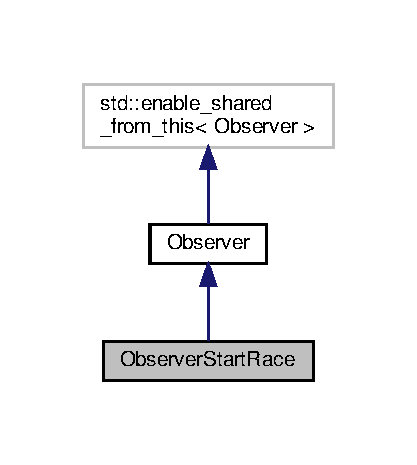
\includegraphics[width=200pt]{classObserverStartRace__inherit__graph}
\end{center}
\end{figure}


Collaboration diagram for Observer\+Start\+Race\+:\nopagebreak
\begin{figure}[H]
\begin{center}
\leavevmode
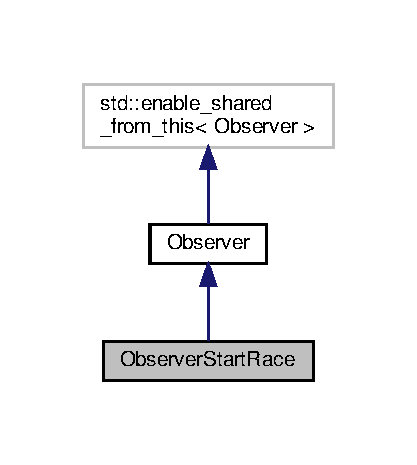
\includegraphics[width=200pt]{classObserverStartRace__coll__graph}
\end{center}
\end{figure}
\subsection*{Public Member Functions}
\begin{DoxyCompactItemize}
\item 
\hyperlink{classObserverStartRace_a663caac255a23d662e1d3631b3ed12a9}{Observer\+Start\+Race} (std\+::shared\+\_\+ptr$<$ sf\+::\+Render\+Window $>$ wind)
\item 
void \hyperlink{classObserverStartRace_aa810164d0877c5597ec06adab29b7981}{update} (int timer) override
\item 
std\+::string \hyperlink{classObserverStartRace_af664693404c9c8f756a8e4ba7d687c3a}{get\+Type} () override
\end{DoxyCompactItemize}


\subsection{Detailed Description}
The observer that handles the timer at the start of every level 

\subsection{Constructor \& Destructor Documentation}
\mbox{\Hypertarget{classObserverStartRace_a663caac255a23d662e1d3631b3ed12a9}\label{classObserverStartRace_a663caac255a23d662e1d3631b3ed12a9}} 
\index{Observer\+Start\+Race@{Observer\+Start\+Race}!Observer\+Start\+Race@{Observer\+Start\+Race}}
\index{Observer\+Start\+Race@{Observer\+Start\+Race}!Observer\+Start\+Race@{Observer\+Start\+Race}}
\subsubsection{\texorpdfstring{Observer\+Start\+Race()}{ObserverStartRace()}}
{\footnotesize\ttfamily Observer\+Start\+Race\+::\+Observer\+Start\+Race (\begin{DoxyParamCaption}\item[{std\+::shared\+\_\+ptr$<$ sf\+::\+Render\+Window $>$}]{wind }\end{DoxyParamCaption})}

Constructor with the sfml window 
\begin{DoxyParams}{Parameters}
{\em wind} & \\
\hline
\end{DoxyParams}


\subsection{Member Function Documentation}
\mbox{\Hypertarget{classObserverStartRace_af664693404c9c8f756a8e4ba7d687c3a}\label{classObserverStartRace_af664693404c9c8f756a8e4ba7d687c3a}} 
\index{Observer\+Start\+Race@{Observer\+Start\+Race}!get\+Type@{get\+Type}}
\index{get\+Type@{get\+Type}!Observer\+Start\+Race@{Observer\+Start\+Race}}
\subsubsection{\texorpdfstring{get\+Type()}{getType()}}
{\footnotesize\ttfamily std\+::string Observer\+Start\+Race\+::get\+Type (\begin{DoxyParamCaption}{ }\end{DoxyParamCaption})\hspace{0.3cm}{\ttfamily [override]}, {\ttfamily [virtual]}}

Returns the type of observer \begin{DoxyReturn}{Returns}

\end{DoxyReturn}


Implements \hyperlink{classObserver_a92f704d0a3e6e0ade2743da2ae91bcb7}{Observer}.

\mbox{\Hypertarget{classObserverStartRace_aa810164d0877c5597ec06adab29b7981}\label{classObserverStartRace_aa810164d0877c5597ec06adab29b7981}} 
\index{Observer\+Start\+Race@{Observer\+Start\+Race}!update@{update}}
\index{update@{update}!Observer\+Start\+Race@{Observer\+Start\+Race}}
\subsubsection{\texorpdfstring{update()}{update()}}
{\footnotesize\ttfamily void Observer\+Start\+Race\+::update (\begin{DoxyParamCaption}\item[{int}]{timer }\end{DoxyParamCaption})\hspace{0.3cm}{\ttfamily [override]}, {\ttfamily [virtual]}}

Updates the observer with the timer 
\begin{DoxyParams}{Parameters}
{\em timer} & \\
\hline
\end{DoxyParams}


Implements \hyperlink{classObserver_a4b9e6fbc74e7ae6971b2afe462ab5a87}{Observer}.



The documentation for this class was generated from the following files\+:\begin{DoxyCompactItemize}
\item 
Observer/Observer\+Start\+Race.\+h\item 
Observer/Observer\+Start\+Race.\+cpp\end{DoxyCompactItemize}

\hypertarget{classroadfighter_1_1PassingCar}{}\section{roadfighter\+:\+:Passing\+Car Class Reference}
\label{classroadfighter_1_1PassingCar}\index{roadfighter\+::\+Passing\+Car@{roadfighter\+::\+Passing\+Car}}


{\ttfamily \#include $<$Passing\+Car.\+h$>$}



Inheritance diagram for roadfighter\+:\+:Passing\+Car\+:\nopagebreak
\begin{figure}[H]
\begin{center}
\leavevmode
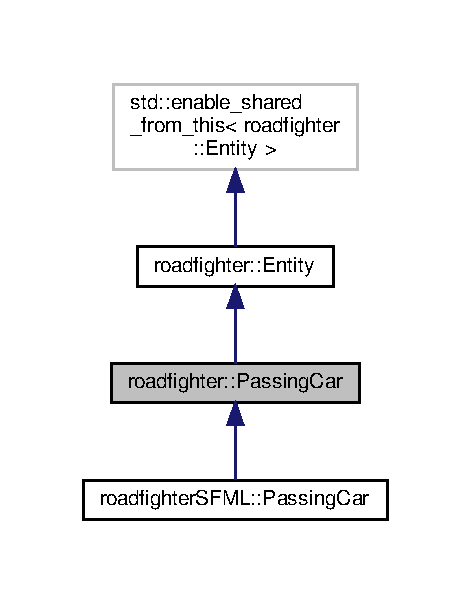
\includegraphics[width=226pt]{classroadfighter_1_1PassingCar__inherit__graph}
\end{center}
\end{figure}


Collaboration diagram for roadfighter\+:\+:Passing\+Car\+:\nopagebreak
\begin{figure}[H]
\begin{center}
\leavevmode
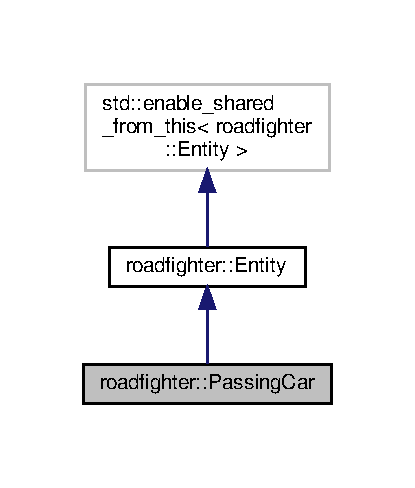
\includegraphics[width=199pt]{classroadfighter_1_1PassingCar__coll__graph}
\end{center}
\end{figure}
\subsection*{Public Member Functions}
\begin{DoxyCompactItemize}
\item 
\hyperlink{classroadfighter_1_1PassingCar_a2f3ae2000521dabcd282f9538b0c87be}{Passing\+Car} (std\+::shared\+\_\+ptr$<$ \hyperlink{classConfigData}{Config\+Data} $>$ config)
\item 
void \hyperlink{classroadfighter_1_1PassingCar_a45276fb9270a145fed9a7827a9ab7a46}{update} () override
\item 
void \hyperlink{classroadfighter_1_1PassingCar_af0667cf430382117beb4669777905cc7}{update} (int \hyperlink{classroadfighter_1_1PassingCar_a7b35bee0a1fd977770e98672583991c5}{speed}, std\+::shared\+\_\+ptr$<$ \hyperlink{classroadfighter_1_1Entity}{roadfighter\+::\+Entity} $>$ Player) override
\item 
int \hyperlink{classroadfighter_1_1PassingCar_afae62d9c6037d5ce8f74bb2e2ed363ac}{get\+Speed} () override
\item 
int \hyperlink{classroadfighter_1_1PassingCar_a1a2838de0992a6e46793d0fe0f128b36}{Delete} () override
\item 
std\+::shared\+\_\+ptr$<$ \hyperlink{structObjBox}{Obj\+Box} $>$ \hyperlink{classroadfighter_1_1PassingCar_aeee1f7e16dcef7adc0a4bea629b0d42b}{get\+Objbox} () override
\item 
void \hyperlink{classroadfighter_1_1PassingCar_aad1905fcb427945c3300840deedffb1d}{set\+Delete} (int del) override
\item 
bool \hyperlink{classroadfighter_1_1PassingCar_a16df11cb6ac5ce29b733d1063490c95c}{Shoot} () override
\end{DoxyCompactItemize}
\subsection*{Protected Attributes}
\begin{DoxyCompactItemize}
\item 
std\+::pair$<$ double, double $>$ \hyperlink{classroadfighter_1_1PassingCar_aa9ba790b7ce315a2b914814b9f4de68a}{centralpos}
\item 
int \hyperlink{classroadfighter_1_1PassingCar_a7b35bee0a1fd977770e98672583991c5}{speed}
\item 
int \hyperlink{classroadfighter_1_1PassingCar_aa1607598fb0724778dc38404313a5b6c}{to\+Del} = 0
\item 
double \hyperlink{classroadfighter_1_1PassingCar_a3fb050dc05c6c20e776ea167a31b199b}{height}
\item 
double \hyperlink{classroadfighter_1_1PassingCar_a5168bee8ec5bd08cd42599738d20ccab}{width}
\end{DoxyCompactItemize}


\subsection{Detailed Description}
Car that the player can pass 

\subsection{Constructor \& Destructor Documentation}
\mbox{\Hypertarget{classroadfighter_1_1PassingCar_a2f3ae2000521dabcd282f9538b0c87be}\label{classroadfighter_1_1PassingCar_a2f3ae2000521dabcd282f9538b0c87be}} 
\index{roadfighter\+::\+Passing\+Car@{roadfighter\+::\+Passing\+Car}!Passing\+Car@{Passing\+Car}}
\index{Passing\+Car@{Passing\+Car}!roadfighter\+::\+Passing\+Car@{roadfighter\+::\+Passing\+Car}}
\subsubsection{\texorpdfstring{Passing\+Car()}{PassingCar()}}
{\footnotesize\ttfamily roadfighter\+::\+Passing\+Car\+::\+Passing\+Car (\begin{DoxyParamCaption}\item[{std\+::shared\+\_\+ptr$<$ \hyperlink{classConfigData}{Config\+Data} $>$}]{config }\end{DoxyParamCaption})}

Constructor with configuration data 
\begin{DoxyParams}{Parameters}
{\em config} & \\
\hline
\end{DoxyParams}


\subsection{Member Function Documentation}
\mbox{\Hypertarget{classroadfighter_1_1PassingCar_a1a2838de0992a6e46793d0fe0f128b36}\label{classroadfighter_1_1PassingCar_a1a2838de0992a6e46793d0fe0f128b36}} 
\index{roadfighter\+::\+Passing\+Car@{roadfighter\+::\+Passing\+Car}!Delete@{Delete}}
\index{Delete@{Delete}!roadfighter\+::\+Passing\+Car@{roadfighter\+::\+Passing\+Car}}
\subsubsection{\texorpdfstring{Delete()}{Delete()}}
{\footnotesize\ttfamily int roadfighter\+::\+Passing\+Car\+::\+Delete (\begin{DoxyParamCaption}{ }\end{DoxyParamCaption})\hspace{0.3cm}{\ttfamily [override]}, {\ttfamily [virtual]}}

Returns a certain value to determine the delete status 0 = nothing, 1 = delete, 2 = respawn \begin{DoxyReturn}{Returns}

\end{DoxyReturn}


Implements \hyperlink{classroadfighter_1_1Entity_a08190b0b8e6a3fcdb42273d6096152ac}{roadfighter\+::\+Entity}.

\mbox{\Hypertarget{classroadfighter_1_1PassingCar_aeee1f7e16dcef7adc0a4bea629b0d42b}\label{classroadfighter_1_1PassingCar_aeee1f7e16dcef7adc0a4bea629b0d42b}} 
\index{roadfighter\+::\+Passing\+Car@{roadfighter\+::\+Passing\+Car}!get\+Objbox@{get\+Objbox}}
\index{get\+Objbox@{get\+Objbox}!roadfighter\+::\+Passing\+Car@{roadfighter\+::\+Passing\+Car}}
\subsubsection{\texorpdfstring{get\+Objbox()}{getObjbox()}}
{\footnotesize\ttfamily std\+::shared\+\_\+ptr$<$ \hyperlink{structObjBox}{Obj\+Box} $>$ roadfighter\+::\+Passing\+Car\+::get\+Objbox (\begin{DoxyParamCaption}{ }\end{DoxyParamCaption})\hspace{0.3cm}{\ttfamily [override]}, {\ttfamily [virtual]}}

Return a shared\+\_\+ptr of the object box \begin{DoxyReturn}{Returns}

\end{DoxyReturn}


Implements \hyperlink{classroadfighter_1_1Entity_af14340d04a725175a6d221f23c35fa0c}{roadfighter\+::\+Entity}.

\mbox{\Hypertarget{classroadfighter_1_1PassingCar_afae62d9c6037d5ce8f74bb2e2ed363ac}\label{classroadfighter_1_1PassingCar_afae62d9c6037d5ce8f74bb2e2ed363ac}} 
\index{roadfighter\+::\+Passing\+Car@{roadfighter\+::\+Passing\+Car}!get\+Speed@{get\+Speed}}
\index{get\+Speed@{get\+Speed}!roadfighter\+::\+Passing\+Car@{roadfighter\+::\+Passing\+Car}}
\subsubsection{\texorpdfstring{get\+Speed()}{getSpeed()}}
{\footnotesize\ttfamily int roadfighter\+::\+Passing\+Car\+::get\+Speed (\begin{DoxyParamCaption}{ }\end{DoxyParamCaption})\hspace{0.3cm}{\ttfamily [override]}, {\ttfamily [virtual]}}

Returns the speed of the object \begin{DoxyReturn}{Returns}
speed 
\end{DoxyReturn}


Implements \hyperlink{classroadfighter_1_1Entity_ad3760184d764a61922e1db7d98501ee4}{roadfighter\+::\+Entity}.

\mbox{\Hypertarget{classroadfighter_1_1PassingCar_aad1905fcb427945c3300840deedffb1d}\label{classroadfighter_1_1PassingCar_aad1905fcb427945c3300840deedffb1d}} 
\index{roadfighter\+::\+Passing\+Car@{roadfighter\+::\+Passing\+Car}!set\+Delete@{set\+Delete}}
\index{set\+Delete@{set\+Delete}!roadfighter\+::\+Passing\+Car@{roadfighter\+::\+Passing\+Car}}
\subsubsection{\texorpdfstring{set\+Delete()}{setDelete()}}
{\footnotesize\ttfamily void roadfighter\+::\+Passing\+Car\+::set\+Delete (\begin{DoxyParamCaption}\item[{int}]{del }\end{DoxyParamCaption})\hspace{0.3cm}{\ttfamily [override]}, {\ttfamily [virtual]}}

Set if an object must be deleted or not 
\begin{DoxyParams}{Parameters}
{\em del} & \\
\hline
\end{DoxyParams}


Implements \hyperlink{classroadfighter_1_1Entity_a07e973f0fa941a69e749629716877692}{roadfighter\+::\+Entity}.

\mbox{\Hypertarget{classroadfighter_1_1PassingCar_a16df11cb6ac5ce29b733d1063490c95c}\label{classroadfighter_1_1PassingCar_a16df11cb6ac5ce29b733d1063490c95c}} 
\index{roadfighter\+::\+Passing\+Car@{roadfighter\+::\+Passing\+Car}!Shoot@{Shoot}}
\index{Shoot@{Shoot}!roadfighter\+::\+Passing\+Car@{roadfighter\+::\+Passing\+Car}}
\subsubsection{\texorpdfstring{Shoot()}{Shoot()}}
{\footnotesize\ttfamily bool roadfighter\+::\+Passing\+Car\+::\+Shoot (\begin{DoxyParamCaption}{ }\end{DoxyParamCaption})\hspace{0.3cm}{\ttfamily [override]}, {\ttfamily [virtual]}}

Return if the object shot \begin{DoxyReturn}{Returns}

\end{DoxyReturn}


Implements \hyperlink{classroadfighter_1_1Entity_ad0ecaa0539db252e591da83814251509}{roadfighter\+::\+Entity}.

\mbox{\Hypertarget{classroadfighter_1_1PassingCar_a45276fb9270a145fed9a7827a9ab7a46}\label{classroadfighter_1_1PassingCar_a45276fb9270a145fed9a7827a9ab7a46}} 
\index{roadfighter\+::\+Passing\+Car@{roadfighter\+::\+Passing\+Car}!update@{update}}
\index{update@{update}!roadfighter\+::\+Passing\+Car@{roadfighter\+::\+Passing\+Car}}
\subsubsection{\texorpdfstring{update()}{update()}\hspace{0.1cm}{\footnotesize\ttfamily [1/2]}}
{\footnotesize\ttfamily void roadfighter\+::\+Passing\+Car\+::update (\begin{DoxyParamCaption}{ }\end{DoxyParamCaption})\hspace{0.3cm}{\ttfamily [override]}, {\ttfamily [virtual]}}

Update 

Implements \hyperlink{classroadfighter_1_1Entity_a19cd353f12a3e8432acd6d5609137561}{roadfighter\+::\+Entity}.

\mbox{\Hypertarget{classroadfighter_1_1PassingCar_af0667cf430382117beb4669777905cc7}\label{classroadfighter_1_1PassingCar_af0667cf430382117beb4669777905cc7}} 
\index{roadfighter\+::\+Passing\+Car@{roadfighter\+::\+Passing\+Car}!update@{update}}
\index{update@{update}!roadfighter\+::\+Passing\+Car@{roadfighter\+::\+Passing\+Car}}
\subsubsection{\texorpdfstring{update()}{update()}\hspace{0.1cm}{\footnotesize\ttfamily [2/2]}}
{\footnotesize\ttfamily void roadfighter\+::\+Passing\+Car\+::update (\begin{DoxyParamCaption}\item[{int}]{speed,  }\item[{std\+::shared\+\_\+ptr$<$ \hyperlink{classroadfighter_1_1Entity}{roadfighter\+::\+Entity} $>$}]{Player }\end{DoxyParamCaption})\hspace{0.3cm}{\ttfamily [override]}, {\ttfamily [virtual]}}

Updates the object with extra parameters 
\begin{DoxyParams}{Parameters}
{\em speed} & \\
\hline
{\em Player} & \\
\hline
\end{DoxyParams}


Implements \hyperlink{classroadfighter_1_1Entity_a611ba56595dd2137d308876ba820cc09}{roadfighter\+::\+Entity}.



\subsection{Member Data Documentation}
\mbox{\Hypertarget{classroadfighter_1_1PassingCar_aa9ba790b7ce315a2b914814b9f4de68a}\label{classroadfighter_1_1PassingCar_aa9ba790b7ce315a2b914814b9f4de68a}} 
\index{roadfighter\+::\+Passing\+Car@{roadfighter\+::\+Passing\+Car}!centralpos@{centralpos}}
\index{centralpos@{centralpos}!roadfighter\+::\+Passing\+Car@{roadfighter\+::\+Passing\+Car}}
\subsubsection{\texorpdfstring{centralpos}{centralpos}}
{\footnotesize\ttfamily std\+::pair$<$double, double$>$ roadfighter\+::\+Passing\+Car\+::centralpos\hspace{0.3cm}{\ttfamily [protected]}}

Pair of the doubles that contains the x and y position of the center of the object \mbox{\Hypertarget{classroadfighter_1_1PassingCar_a3fb050dc05c6c20e776ea167a31b199b}\label{classroadfighter_1_1PassingCar_a3fb050dc05c6c20e776ea167a31b199b}} 
\index{roadfighter\+::\+Passing\+Car@{roadfighter\+::\+Passing\+Car}!height@{height}}
\index{height@{height}!roadfighter\+::\+Passing\+Car@{roadfighter\+::\+Passing\+Car}}
\subsubsection{\texorpdfstring{height}{height}}
{\footnotesize\ttfamily double roadfighter\+::\+Passing\+Car\+::height\hspace{0.3cm}{\ttfamily [protected]}}

Height of the object \mbox{\Hypertarget{classroadfighter_1_1PassingCar_a7b35bee0a1fd977770e98672583991c5}\label{classroadfighter_1_1PassingCar_a7b35bee0a1fd977770e98672583991c5}} 
\index{roadfighter\+::\+Passing\+Car@{roadfighter\+::\+Passing\+Car}!speed@{speed}}
\index{speed@{speed}!roadfighter\+::\+Passing\+Car@{roadfighter\+::\+Passing\+Car}}
\subsubsection{\texorpdfstring{speed}{speed}}
{\footnotesize\ttfamily int roadfighter\+::\+Passing\+Car\+::speed\hspace{0.3cm}{\ttfamily [protected]}}

Speed of the object \mbox{\Hypertarget{classroadfighter_1_1PassingCar_aa1607598fb0724778dc38404313a5b6c}\label{classroadfighter_1_1PassingCar_aa1607598fb0724778dc38404313a5b6c}} 
\index{roadfighter\+::\+Passing\+Car@{roadfighter\+::\+Passing\+Car}!to\+Del@{to\+Del}}
\index{to\+Del@{to\+Del}!roadfighter\+::\+Passing\+Car@{roadfighter\+::\+Passing\+Car}}
\subsubsection{\texorpdfstring{to\+Del}{toDel}}
{\footnotesize\ttfamily int roadfighter\+::\+Passing\+Car\+::to\+Del = 0\hspace{0.3cm}{\ttfamily [protected]}}

Object deletion status ( 0 = nothing, 1 = delete, 2 = respawn ) \mbox{\Hypertarget{classroadfighter_1_1PassingCar_a5168bee8ec5bd08cd42599738d20ccab}\label{classroadfighter_1_1PassingCar_a5168bee8ec5bd08cd42599738d20ccab}} 
\index{roadfighter\+::\+Passing\+Car@{roadfighter\+::\+Passing\+Car}!width@{width}}
\index{width@{width}!roadfighter\+::\+Passing\+Car@{roadfighter\+::\+Passing\+Car}}
\subsubsection{\texorpdfstring{width}{width}}
{\footnotesize\ttfamily double roadfighter\+::\+Passing\+Car\+::width\hspace{0.3cm}{\ttfamily [protected]}}

Width of the object 

The documentation for this class was generated from the following files\+:\begin{DoxyCompactItemize}
\item 
roadfighter/Passing\+Car.\+h\item 
roadfighter/Passing\+Car.\+cpp\end{DoxyCompactItemize}

\hypertarget{classroadfighterSFML_1_1PassingCar}{}\section{roadfighter\+S\+F\+ML\+:\+:Passing\+Car Class Reference}
\label{classroadfighterSFML_1_1PassingCar}\index{roadfighter\+S\+F\+M\+L\+::\+Passing\+Car@{roadfighter\+S\+F\+M\+L\+::\+Passing\+Car}}


{\ttfamily \#include $<$Passing\+Car.\+h$>$}



Inheritance diagram for roadfighter\+S\+F\+ML\+:\+:Passing\+Car\+:\nopagebreak
\begin{figure}[H]
\begin{center}
\leavevmode
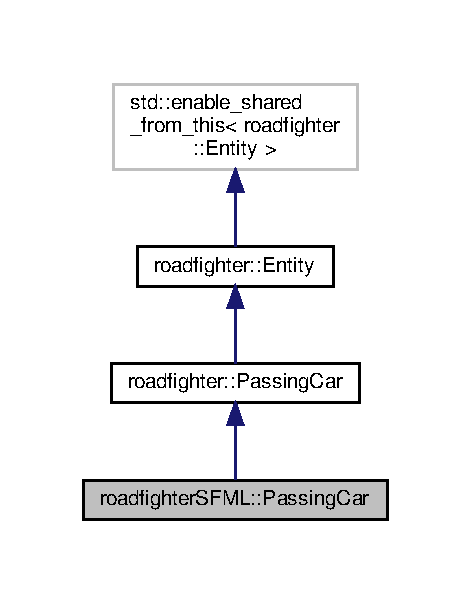
\includegraphics[width=226pt]{classroadfighterSFML_1_1PassingCar__inherit__graph}
\end{center}
\end{figure}


Collaboration diagram for roadfighter\+S\+F\+ML\+:\+:Passing\+Car\+:\nopagebreak
\begin{figure}[H]
\begin{center}
\leavevmode
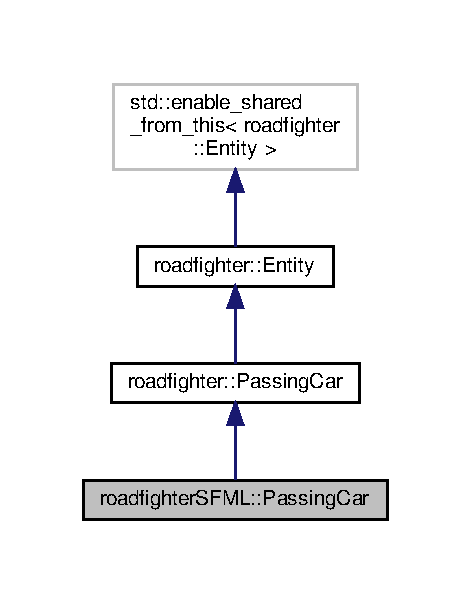
\includegraphics[width=226pt]{classroadfighterSFML_1_1PassingCar__coll__graph}
\end{center}
\end{figure}
\subsection*{Public Member Functions}
\begin{DoxyCompactItemize}
\item 
\hyperlink{classroadfighterSFML_1_1PassingCar_ab8a4b6bb0309aa9ca0d4df67b0fa12a3}{Passing\+Car} (const std\+::shared\+\_\+ptr$<$ sf\+::\+Render\+Window $>$ window, double random, std\+::shared\+\_\+ptr$<$ \hyperlink{classConfigData}{Config\+Data} $>$ config)
\item 
void \hyperlink{classroadfighterSFML_1_1PassingCar_ae8d3cff5198ad85dde5ab864b0528337}{draw} () override
\end{DoxyCompactItemize}
\subsection*{Additional Inherited Members}


\subsection{Detailed Description}
Graphic side of passingcar 

\subsection{Constructor \& Destructor Documentation}
\mbox{\Hypertarget{classroadfighterSFML_1_1PassingCar_ab8a4b6bb0309aa9ca0d4df67b0fa12a3}\label{classroadfighterSFML_1_1PassingCar_ab8a4b6bb0309aa9ca0d4df67b0fa12a3}} 
\index{roadfighter\+S\+F\+M\+L\+::\+Passing\+Car@{roadfighter\+S\+F\+M\+L\+::\+Passing\+Car}!Passing\+Car@{Passing\+Car}}
\index{Passing\+Car@{Passing\+Car}!roadfighter\+S\+F\+M\+L\+::\+Passing\+Car@{roadfighter\+S\+F\+M\+L\+::\+Passing\+Car}}
\subsubsection{\texorpdfstring{Passing\+Car()}{PassingCar()}}
{\footnotesize\ttfamily roadfighter\+S\+F\+M\+L\+::\+Passing\+Car\+::\+Passing\+Car (\begin{DoxyParamCaption}\item[{const std\+::shared\+\_\+ptr$<$ sf\+::\+Render\+Window $>$}]{window,  }\item[{double}]{random,  }\item[{std\+::shared\+\_\+ptr$<$ \hyperlink{classConfigData}{Config\+Data} $>$}]{config }\end{DoxyParamCaption})}

Constructor with window and a random value to determine the spawning location and configuration data 
\begin{DoxyParams}{Parameters}
{\em window} & \\
\hline
{\em random} & \\
\hline
{\em config} & \\
\hline
\end{DoxyParams}


\subsection{Member Function Documentation}
\mbox{\Hypertarget{classroadfighterSFML_1_1PassingCar_ae8d3cff5198ad85dde5ab864b0528337}\label{classroadfighterSFML_1_1PassingCar_ae8d3cff5198ad85dde5ab864b0528337}} 
\index{roadfighter\+S\+F\+M\+L\+::\+Passing\+Car@{roadfighter\+S\+F\+M\+L\+::\+Passing\+Car}!draw@{draw}}
\index{draw@{draw}!roadfighter\+S\+F\+M\+L\+::\+Passing\+Car@{roadfighter\+S\+F\+M\+L\+::\+Passing\+Car}}
\subsubsection{\texorpdfstring{draw()}{draw()}}
{\footnotesize\ttfamily void roadfighter\+S\+F\+M\+L\+::\+Passing\+Car\+::draw (\begin{DoxyParamCaption}{ }\end{DoxyParamCaption})\hspace{0.3cm}{\ttfamily [override]}, {\ttfamily [virtual]}}

Draws the object 

Implements \hyperlink{classroadfighter_1_1Entity_ac516f8005f969ad5a86c252e5a3640ee}{roadfighter\+::\+Entity}.



The documentation for this class was generated from the following files\+:\begin{DoxyCompactItemize}
\item 
roadfighter\+S\+F\+M\+L/Passing\+Car.\+h\item 
roadfighter\+S\+F\+M\+L/Passing\+Car.\+cpp\end{DoxyCompactItemize}

\hypertarget{classroadfighterSFML_1_1PlayerCar}{}\section{roadfighter\+S\+F\+ML\+:\+:Player\+Car Class Reference}
\label{classroadfighterSFML_1_1PlayerCar}\index{roadfighter\+S\+F\+M\+L\+::\+Player\+Car@{roadfighter\+S\+F\+M\+L\+::\+Player\+Car}}


{\ttfamily \#include $<$Player\+Car.\+h$>$}



Inheritance diagram for roadfighter\+S\+F\+ML\+:\+:Player\+Car\+:\nopagebreak
\begin{figure}[H]
\begin{center}
\leavevmode
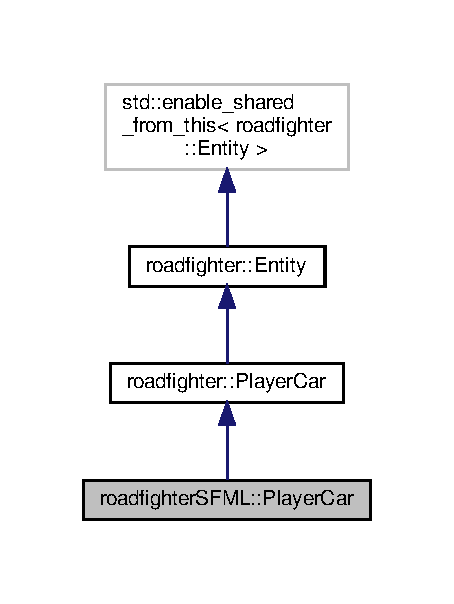
\includegraphics[width=218pt]{classroadfighterSFML_1_1PlayerCar__inherit__graph}
\end{center}
\end{figure}


Collaboration diagram for roadfighter\+S\+F\+ML\+:\+:Player\+Car\+:\nopagebreak
\begin{figure}[H]
\begin{center}
\leavevmode
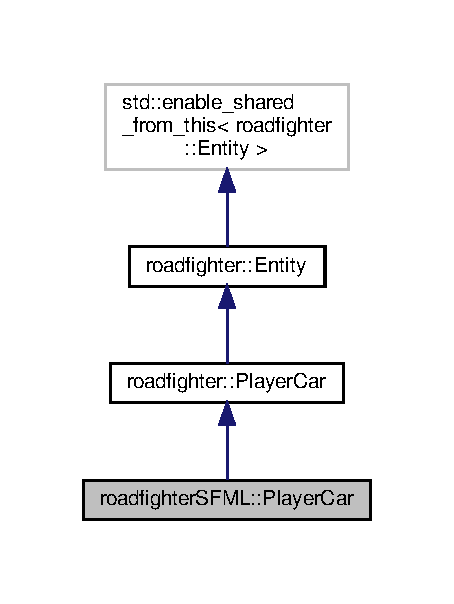
\includegraphics[width=218pt]{classroadfighterSFML_1_1PlayerCar__coll__graph}
\end{center}
\end{figure}
\subsection*{Public Member Functions}
\begin{DoxyCompactItemize}
\item 
\hyperlink{classroadfighterSFML_1_1PlayerCar_a4fc864a63655f04a3c4144b70214b4b1}{Player\+Car} (const std\+::shared\+\_\+ptr$<$ sf\+::\+Render\+Window $>$ window, int \hyperlink{classroadfighter_1_1PlayerCar_ac198b0404bf9105cf835bf25303e63db}{level}, std\+::shared\+\_\+ptr$<$ \hyperlink{classConfigData}{Config\+Data} $>$ config)
\item 
void \hyperlink{classroadfighterSFML_1_1PlayerCar_a9676cb8164bbc20f2ddedccf73ec5ef8}{draw} () override
\item 
void \hyperlink{classroadfighterSFML_1_1PlayerCar_a1fb9b80b068e689bef90cad28c53869c}{update} () override
\end{DoxyCompactItemize}
\subsection*{Additional Inherited Members}


\subsection{Detailed Description}
Graphic side of the player class 

\subsection{Constructor \& Destructor Documentation}
\mbox{\Hypertarget{classroadfighterSFML_1_1PlayerCar_a4fc864a63655f04a3c4144b70214b4b1}\label{classroadfighterSFML_1_1PlayerCar_a4fc864a63655f04a3c4144b70214b4b1}} 
\index{roadfighter\+S\+F\+M\+L\+::\+Player\+Car@{roadfighter\+S\+F\+M\+L\+::\+Player\+Car}!Player\+Car@{Player\+Car}}
\index{Player\+Car@{Player\+Car}!roadfighter\+S\+F\+M\+L\+::\+Player\+Car@{roadfighter\+S\+F\+M\+L\+::\+Player\+Car}}
\subsubsection{\texorpdfstring{Player\+Car()}{PlayerCar()}}
{\footnotesize\ttfamily roadfighter\+S\+F\+M\+L\+::\+Player\+Car\+::\+Player\+Car (\begin{DoxyParamCaption}\item[{const std\+::shared\+\_\+ptr$<$ sf\+::\+Render\+Window $>$}]{window,  }\item[{int}]{level,  }\item[{std\+::shared\+\_\+ptr$<$ \hyperlink{classConfigData}{Config\+Data} $>$}]{config }\end{DoxyParamCaption})}

Constructor with sfml window, current level and configuration data 
\begin{DoxyParams}{Parameters}
{\em window} & \\
\hline
{\em level} & \\
\hline
{\em config} & \\
\hline
\end{DoxyParams}


\subsection{Member Function Documentation}
\mbox{\Hypertarget{classroadfighterSFML_1_1PlayerCar_a9676cb8164bbc20f2ddedccf73ec5ef8}\label{classroadfighterSFML_1_1PlayerCar_a9676cb8164bbc20f2ddedccf73ec5ef8}} 
\index{roadfighter\+S\+F\+M\+L\+::\+Player\+Car@{roadfighter\+S\+F\+M\+L\+::\+Player\+Car}!draw@{draw}}
\index{draw@{draw}!roadfighter\+S\+F\+M\+L\+::\+Player\+Car@{roadfighter\+S\+F\+M\+L\+::\+Player\+Car}}
\subsubsection{\texorpdfstring{draw()}{draw()}}
{\footnotesize\ttfamily void roadfighter\+S\+F\+M\+L\+::\+Player\+Car\+::draw (\begin{DoxyParamCaption}{ }\end{DoxyParamCaption})\hspace{0.3cm}{\ttfamily [override]}, {\ttfamily [virtual]}}

Draws the player 

Implements \hyperlink{classroadfighter_1_1Entity_ac516f8005f969ad5a86c252e5a3640ee}{roadfighter\+::\+Entity}.

\mbox{\Hypertarget{classroadfighterSFML_1_1PlayerCar_a1fb9b80b068e689bef90cad28c53869c}\label{classroadfighterSFML_1_1PlayerCar_a1fb9b80b068e689bef90cad28c53869c}} 
\index{roadfighter\+S\+F\+M\+L\+::\+Player\+Car@{roadfighter\+S\+F\+M\+L\+::\+Player\+Car}!update@{update}}
\index{update@{update}!roadfighter\+S\+F\+M\+L\+::\+Player\+Car@{roadfighter\+S\+F\+M\+L\+::\+Player\+Car}}
\subsubsection{\texorpdfstring{update()}{update()}}
{\footnotesize\ttfamily void roadfighter\+S\+F\+M\+L\+::\+Player\+Car\+::update (\begin{DoxyParamCaption}{ }\end{DoxyParamCaption})\hspace{0.3cm}{\ttfamily [override]}, {\ttfamily [virtual]}}

Updates the player 

Reimplemented from \hyperlink{classroadfighter_1_1PlayerCar_a47772fa1d9fcdba69f288112d5359acd}{roadfighter\+::\+Player\+Car}.



The documentation for this class was generated from the following files\+:\begin{DoxyCompactItemize}
\item 
roadfighter\+S\+F\+M\+L/Player\+Car.\+h\item 
roadfighter\+S\+F\+M\+L/Player\+Car.\+cpp\end{DoxyCompactItemize}

\hypertarget{classroadfighter_1_1PlayerCar}{}\section{roadfighter\+:\+:Player\+Car Class Reference}
\label{classroadfighter_1_1PlayerCar}\index{roadfighter\+::\+Player\+Car@{roadfighter\+::\+Player\+Car}}


{\ttfamily \#include $<$Player\+Car.\+h$>$}



Inheritance diagram for roadfighter\+:\+:Player\+Car\+:\nopagebreak
\begin{figure}[H]
\begin{center}
\leavevmode
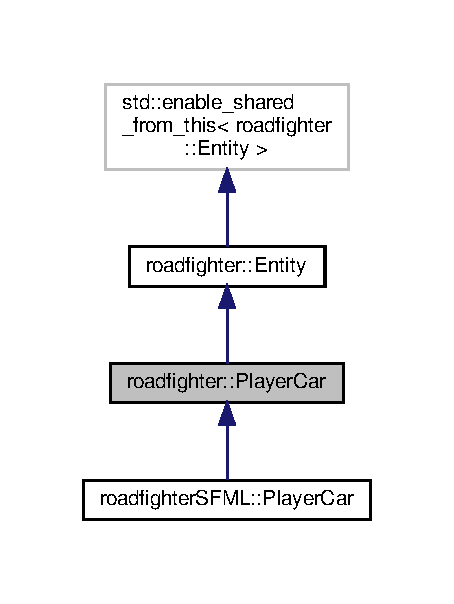
\includegraphics[width=218pt]{classroadfighter_1_1PlayerCar__inherit__graph}
\end{center}
\end{figure}


Collaboration diagram for roadfighter\+:\+:Player\+Car\+:\nopagebreak
\begin{figure}[H]
\begin{center}
\leavevmode
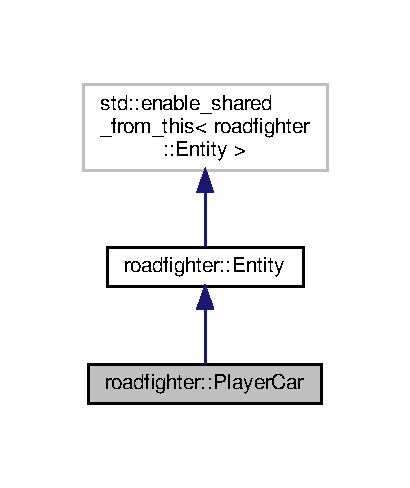
\includegraphics[width=197pt]{classroadfighter_1_1PlayerCar__coll__graph}
\end{center}
\end{figure}
\subsection*{Public Member Functions}
\begin{DoxyCompactItemize}
\item 
\hyperlink{classroadfighter_1_1PlayerCar_a9e0ee387eaede6b742174877c1d594d4}{Player\+Car} (std\+::shared\+\_\+ptr$<$ \hyperlink{classConfigData}{Config\+Data} $>$ config)
\item 
void \hyperlink{classroadfighter_1_1PlayerCar_a65daed6d30d8b65f368779eaa43714e2}{update} (int \hyperlink{classroadfighter_1_1PlayerCar_a0e6307f59c765c9b88ec2b1f0f8f07fc}{speed}, std\+::shared\+\_\+ptr$<$ \hyperlink{classroadfighter_1_1Entity}{roadfighter\+::\+Entity} $>$ Player) override
\item 
int \hyperlink{classroadfighter_1_1PlayerCar_a642a825b604a407ae4711bdafd054b22}{get\+Speed} () override
\item 
int \hyperlink{classroadfighter_1_1PlayerCar_a1c4a181eee7a89315680eca4892ebc32}{Delete} () override
\item 
std\+::shared\+\_\+ptr$<$ \hyperlink{structObjBox}{Obj\+Box} $>$ \hyperlink{classroadfighter_1_1PlayerCar_ac0b95a6ef2829905ad4717a52b7cb5eb}{get\+Objbox} () override
\item 
void \hyperlink{classroadfighter_1_1PlayerCar_a24401332a8585b0fcfbfd33df93021e0}{set\+Delete} (int del) override
\item 
bool \hyperlink{classroadfighter_1_1PlayerCar_af9e034824497fb287085be08c3995733}{Shoot} () override
\item 
void \hyperlink{classroadfighter_1_1PlayerCar_a47772fa1d9fcdba69f288112d5359acd}{update} () override
\end{DoxyCompactItemize}
\subsection*{Protected Member Functions}
\begin{DoxyCompactItemize}
\item 
void \hyperlink{classroadfighter_1_1PlayerCar_a2aa6cf43ac6cf7834d1f854d33fc5e0d}{Update\+Movement} (std\+::vector$<$ std\+::string $>$ inputs)
\item 
void \hyperlink{classroadfighter_1_1PlayerCar_af6a39916181bce4cab033d0b4370cfba}{move} (std\+::string input)
\end{DoxyCompactItemize}
\subsection*{Protected Attributes}
\begin{DoxyCompactItemize}
\item 
std\+::pair$<$ double, double $>$ \hyperlink{classroadfighter_1_1PlayerCar_acc6e2a39d0421a4dcfb50e22d9a1b961}{centralpos} = \{-\/0.\+9, -\/2\}
\item 
int \hyperlink{classroadfighter_1_1PlayerCar_a0e6307f59c765c9b88ec2b1f0f8f07fc}{speed} = 0
\item 
int \hyperlink{classroadfighter_1_1PlayerCar_ae597eb0dcbff6ceccc5dd43d202503a4}{max\+Speed}
\item 
bool \hyperlink{classroadfighter_1_1PlayerCar_a57eeee2b8052155f25f37c0343ea0ecc}{shoot} = false
\item 
int \hyperlink{classroadfighter_1_1PlayerCar_a97dc2e80fcacfe2fabdb4684de15e19b}{reload}
\item 
int \hyperlink{classroadfighter_1_1PlayerCar_ae4043388c6399f4a1341b9e9b879ba0a}{reloadval}
\item 
bool \hyperlink{classroadfighter_1_1PlayerCar_a9ee8c58f93057786b6d184ed73636c14}{reloading} = false
\item 
int \hyperlink{classroadfighter_1_1PlayerCar_a44cdcc6dea044b424d852dc01b8728f1}{to\+Del} = 0
\item 
double \hyperlink{classroadfighter_1_1PlayerCar_aa1e63b489ae2b5400fdd159fcea03417}{height}
\item 
double \hyperlink{classroadfighter_1_1PlayerCar_aeb7ba30397f5c61a94f4630d8ac1d2c9}{width}
\item 
int \hyperlink{classroadfighter_1_1PlayerCar_a57dd797c06cab823a4210eb73aed07b7}{Car\+Travelled\+Distance} = 0
\item 
bool \hyperlink{classroadfighter_1_1PlayerCar_a4b35caad02ea04a6acc0c8e9e649bce3}{finished} = false
\item 
int \hyperlink{classroadfighter_1_1PlayerCar_af50c73327950a35fe1d906246cc9b008}{respawntimer}
\item 
int \hyperlink{classroadfighter_1_1PlayerCar_aca1f3db779c605745f92e72c08925a7e}{respawntimer\+Val}
\item 
bool \hyperlink{classroadfighter_1_1PlayerCar_ac2b0e5cd761fb485853c288080a66b6d}{disable\+Actions} = false
\item 
int \hyperlink{classroadfighter_1_1PlayerCar_ac198b0404bf9105cf835bf25303e63db}{level}
\item 
bool \hyperlink{classroadfighter_1_1PlayerCar_a3dfbd9298fcfc470d4583778eaebe67b}{bossfight} = false
\item 
int \hyperlink{classroadfighter_1_1PlayerCar_accc524af68300b7b817d11ea2b989890}{acceleration}
\end{DoxyCompactItemize}


\subsection{Detailed Description}
The player that can be controlled 

\subsection{Constructor \& Destructor Documentation}
\mbox{\Hypertarget{classroadfighter_1_1PlayerCar_a9e0ee387eaede6b742174877c1d594d4}\label{classroadfighter_1_1PlayerCar_a9e0ee387eaede6b742174877c1d594d4}} 
\index{roadfighter\+::\+Player\+Car@{roadfighter\+::\+Player\+Car}!Player\+Car@{Player\+Car}}
\index{Player\+Car@{Player\+Car}!roadfighter\+::\+Player\+Car@{roadfighter\+::\+Player\+Car}}
\subsubsection{\texorpdfstring{Player\+Car()}{PlayerCar()}}
{\footnotesize\ttfamily roadfighter\+::\+Player\+Car\+::\+Player\+Car (\begin{DoxyParamCaption}\item[{std\+::shared\+\_\+ptr$<$ \hyperlink{classConfigData}{Config\+Data} $>$}]{config }\end{DoxyParamCaption})}

Constructor with configuration data 
\begin{DoxyParams}{Parameters}
{\em config} & \\
\hline
\end{DoxyParams}


\subsection{Member Function Documentation}
\mbox{\Hypertarget{classroadfighter_1_1PlayerCar_a1c4a181eee7a89315680eca4892ebc32}\label{classroadfighter_1_1PlayerCar_a1c4a181eee7a89315680eca4892ebc32}} 
\index{roadfighter\+::\+Player\+Car@{roadfighter\+::\+Player\+Car}!Delete@{Delete}}
\index{Delete@{Delete}!roadfighter\+::\+Player\+Car@{roadfighter\+::\+Player\+Car}}
\subsubsection{\texorpdfstring{Delete()}{Delete()}}
{\footnotesize\ttfamily int roadfighter\+::\+Player\+Car\+::\+Delete (\begin{DoxyParamCaption}{ }\end{DoxyParamCaption})\hspace{0.3cm}{\ttfamily [override]}, {\ttfamily [virtual]}}

Return if the object has to be deletes \begin{DoxyReturn}{Returns}

\end{DoxyReturn}


Implements \hyperlink{classroadfighter_1_1Entity_a08190b0b8e6a3fcdb42273d6096152ac}{roadfighter\+::\+Entity}.

\mbox{\Hypertarget{classroadfighter_1_1PlayerCar_ac0b95a6ef2829905ad4717a52b7cb5eb}\label{classroadfighter_1_1PlayerCar_ac0b95a6ef2829905ad4717a52b7cb5eb}} 
\index{roadfighter\+::\+Player\+Car@{roadfighter\+::\+Player\+Car}!get\+Objbox@{get\+Objbox}}
\index{get\+Objbox@{get\+Objbox}!roadfighter\+::\+Player\+Car@{roadfighter\+::\+Player\+Car}}
\subsubsection{\texorpdfstring{get\+Objbox()}{getObjbox()}}
{\footnotesize\ttfamily std\+::shared\+\_\+ptr$<$ \hyperlink{structObjBox}{Obj\+Box} $>$ roadfighter\+::\+Player\+Car\+::get\+Objbox (\begin{DoxyParamCaption}{ }\end{DoxyParamCaption})\hspace{0.3cm}{\ttfamily [override]}, {\ttfamily [virtual]}}

Returns a shared\+\_\+ptr of the object box \begin{DoxyReturn}{Returns}

\end{DoxyReturn}


Implements \hyperlink{classroadfighter_1_1Entity_af14340d04a725175a6d221f23c35fa0c}{roadfighter\+::\+Entity}.

\mbox{\Hypertarget{classroadfighter_1_1PlayerCar_a642a825b604a407ae4711bdafd054b22}\label{classroadfighter_1_1PlayerCar_a642a825b604a407ae4711bdafd054b22}} 
\index{roadfighter\+::\+Player\+Car@{roadfighter\+::\+Player\+Car}!get\+Speed@{get\+Speed}}
\index{get\+Speed@{get\+Speed}!roadfighter\+::\+Player\+Car@{roadfighter\+::\+Player\+Car}}
\subsubsection{\texorpdfstring{get\+Speed()}{getSpeed()}}
{\footnotesize\ttfamily int roadfighter\+::\+Player\+Car\+::get\+Speed (\begin{DoxyParamCaption}{ }\end{DoxyParamCaption})\hspace{0.3cm}{\ttfamily [override]}, {\ttfamily [virtual]}}

Returns the speed of the object \begin{DoxyReturn}{Returns}
speed 
\end{DoxyReturn}


Implements \hyperlink{classroadfighter_1_1Entity_ad3760184d764a61922e1db7d98501ee4}{roadfighter\+::\+Entity}.

\mbox{\Hypertarget{classroadfighter_1_1PlayerCar_af6a39916181bce4cab033d0b4370cfba}\label{classroadfighter_1_1PlayerCar_af6a39916181bce4cab033d0b4370cfba}} 
\index{roadfighter\+::\+Player\+Car@{roadfighter\+::\+Player\+Car}!move@{move}}
\index{move@{move}!roadfighter\+::\+Player\+Car@{roadfighter\+::\+Player\+Car}}
\subsubsection{\texorpdfstring{move()}{move()}}
{\footnotesize\ttfamily void roadfighter\+::\+Player\+Car\+::move (\begin{DoxyParamCaption}\item[{std\+::string}]{input }\end{DoxyParamCaption})\hspace{0.3cm}{\ttfamily [protected]}}

Moves the object left or right depenting on inputs 
\begin{DoxyParams}{Parameters}
{\em input} & \\
\hline
\end{DoxyParams}
\mbox{\Hypertarget{classroadfighter_1_1PlayerCar_a24401332a8585b0fcfbfd33df93021e0}\label{classroadfighter_1_1PlayerCar_a24401332a8585b0fcfbfd33df93021e0}} 
\index{roadfighter\+::\+Player\+Car@{roadfighter\+::\+Player\+Car}!set\+Delete@{set\+Delete}}
\index{set\+Delete@{set\+Delete}!roadfighter\+::\+Player\+Car@{roadfighter\+::\+Player\+Car}}
\subsubsection{\texorpdfstring{set\+Delete()}{setDelete()}}
{\footnotesize\ttfamily void roadfighter\+::\+Player\+Car\+::set\+Delete (\begin{DoxyParamCaption}\item[{int}]{del }\end{DoxyParamCaption})\hspace{0.3cm}{\ttfamily [override]}, {\ttfamily [virtual]}}

Set if the object must be deleted 
\begin{DoxyParams}{Parameters}
{\em del} & \\
\hline
\end{DoxyParams}


Implements \hyperlink{classroadfighter_1_1Entity_a07e973f0fa941a69e749629716877692}{roadfighter\+::\+Entity}.

\mbox{\Hypertarget{classroadfighter_1_1PlayerCar_af9e034824497fb287085be08c3995733}\label{classroadfighter_1_1PlayerCar_af9e034824497fb287085be08c3995733}} 
\index{roadfighter\+::\+Player\+Car@{roadfighter\+::\+Player\+Car}!Shoot@{Shoot}}
\index{Shoot@{Shoot}!roadfighter\+::\+Player\+Car@{roadfighter\+::\+Player\+Car}}
\subsubsection{\texorpdfstring{Shoot()}{Shoot()}}
{\footnotesize\ttfamily bool roadfighter\+::\+Player\+Car\+::\+Shoot (\begin{DoxyParamCaption}{ }\end{DoxyParamCaption})\hspace{0.3cm}{\ttfamily [override]}, {\ttfamily [virtual]}}

Return if the object shot \begin{DoxyReturn}{Returns}

\end{DoxyReturn}


Implements \hyperlink{classroadfighter_1_1Entity_ad0ecaa0539db252e591da83814251509}{roadfighter\+::\+Entity}.

\mbox{\Hypertarget{classroadfighter_1_1PlayerCar_a65daed6d30d8b65f368779eaa43714e2}\label{classroadfighter_1_1PlayerCar_a65daed6d30d8b65f368779eaa43714e2}} 
\index{roadfighter\+::\+Player\+Car@{roadfighter\+::\+Player\+Car}!update@{update}}
\index{update@{update}!roadfighter\+::\+Player\+Car@{roadfighter\+::\+Player\+Car}}
\subsubsection{\texorpdfstring{update()}{update()}\hspace{0.1cm}{\footnotesize\ttfamily [1/2]}}
{\footnotesize\ttfamily void roadfighter\+::\+Player\+Car\+::update (\begin{DoxyParamCaption}\item[{int}]{speed,  }\item[{std\+::shared\+\_\+ptr$<$ \hyperlink{classroadfighter_1_1Entity}{roadfighter\+::\+Entity} $>$}]{Player }\end{DoxyParamCaption})\hspace{0.3cm}{\ttfamily [override]}, {\ttfamily [virtual]}}

Updates the object with extra parameters this function is not used since we already have the needed parameters


\begin{DoxyParams}{Parameters}
{\em speed} & \\
\hline
{\em Player} & \\
\hline
\end{DoxyParams}


Implements \hyperlink{classroadfighter_1_1Entity_a611ba56595dd2137d308876ba820cc09}{roadfighter\+::\+Entity}.

\mbox{\Hypertarget{classroadfighter_1_1PlayerCar_a47772fa1d9fcdba69f288112d5359acd}\label{classroadfighter_1_1PlayerCar_a47772fa1d9fcdba69f288112d5359acd}} 
\index{roadfighter\+::\+Player\+Car@{roadfighter\+::\+Player\+Car}!update@{update}}
\index{update@{update}!roadfighter\+::\+Player\+Car@{roadfighter\+::\+Player\+Car}}
\subsubsection{\texorpdfstring{update()}{update()}\hspace{0.1cm}{\footnotesize\ttfamily [2/2]}}
{\footnotesize\ttfamily void roadfighter\+::\+Player\+Car\+::update (\begin{DoxyParamCaption}{ }\end{DoxyParamCaption})\hspace{0.3cm}{\ttfamily [override]}, {\ttfamily [virtual]}}

Update function that controls bossfight, respawn and finish 

Implements \hyperlink{classroadfighter_1_1Entity_a19cd353f12a3e8432acd6d5609137561}{roadfighter\+::\+Entity}.



Reimplemented in \hyperlink{classroadfighterSFML_1_1PlayerCar_a1fb9b80b068e689bef90cad28c53869c}{roadfighter\+S\+F\+M\+L\+::\+Player\+Car}.

\mbox{\Hypertarget{classroadfighter_1_1PlayerCar_a2aa6cf43ac6cf7834d1f854d33fc5e0d}\label{classroadfighter_1_1PlayerCar_a2aa6cf43ac6cf7834d1f854d33fc5e0d}} 
\index{roadfighter\+::\+Player\+Car@{roadfighter\+::\+Player\+Car}!Update\+Movement@{Update\+Movement}}
\index{Update\+Movement@{Update\+Movement}!roadfighter\+::\+Player\+Car@{roadfighter\+::\+Player\+Car}}
\subsubsection{\texorpdfstring{Update\+Movement()}{UpdateMovement()}}
{\footnotesize\ttfamily void roadfighter\+::\+Player\+Car\+::\+Update\+Movement (\begin{DoxyParamCaption}\item[{std\+::vector$<$ std\+::string $>$}]{inputs }\end{DoxyParamCaption})\hspace{0.3cm}{\ttfamily [protected]}}

Updates the movements depending on the inputs 
\begin{DoxyParams}{Parameters}
{\em inputs} & \\
\hline
\end{DoxyParams}


\subsection{Member Data Documentation}
\mbox{\Hypertarget{classroadfighter_1_1PlayerCar_accc524af68300b7b817d11ea2b989890}\label{classroadfighter_1_1PlayerCar_accc524af68300b7b817d11ea2b989890}} 
\index{roadfighter\+::\+Player\+Car@{roadfighter\+::\+Player\+Car}!acceleration@{acceleration}}
\index{acceleration@{acceleration}!roadfighter\+::\+Player\+Car@{roadfighter\+::\+Player\+Car}}
\subsubsection{\texorpdfstring{acceleration}{acceleration}}
{\footnotesize\ttfamily int roadfighter\+::\+Player\+Car\+::acceleration\hspace{0.3cm}{\ttfamily [protected]}}

Acceleration of the player \mbox{\Hypertarget{classroadfighter_1_1PlayerCar_a3dfbd9298fcfc470d4583778eaebe67b}\label{classroadfighter_1_1PlayerCar_a3dfbd9298fcfc470d4583778eaebe67b}} 
\index{roadfighter\+::\+Player\+Car@{roadfighter\+::\+Player\+Car}!bossfight@{bossfight}}
\index{bossfight@{bossfight}!roadfighter\+::\+Player\+Car@{roadfighter\+::\+Player\+Car}}
\subsubsection{\texorpdfstring{bossfight}{bossfight}}
{\footnotesize\ttfamily bool roadfighter\+::\+Player\+Car\+::bossfight = false\hspace{0.3cm}{\ttfamily [protected]}}

Boolean that is true if we are in bossfight \mbox{\Hypertarget{classroadfighter_1_1PlayerCar_a57dd797c06cab823a4210eb73aed07b7}\label{classroadfighter_1_1PlayerCar_a57dd797c06cab823a4210eb73aed07b7}} 
\index{roadfighter\+::\+Player\+Car@{roadfighter\+::\+Player\+Car}!Car\+Travelled\+Distance@{Car\+Travelled\+Distance}}
\index{Car\+Travelled\+Distance@{Car\+Travelled\+Distance}!roadfighter\+::\+Player\+Car@{roadfighter\+::\+Player\+Car}}
\subsubsection{\texorpdfstring{Car\+Travelled\+Distance}{CarTravelledDistance}}
{\footnotesize\ttfamily int roadfighter\+::\+Player\+Car\+::\+Car\+Travelled\+Distance = 0\hspace{0.3cm}{\ttfamily [protected]}}

Distance that the car travelled \mbox{\Hypertarget{classroadfighter_1_1PlayerCar_acc6e2a39d0421a4dcfb50e22d9a1b961}\label{classroadfighter_1_1PlayerCar_acc6e2a39d0421a4dcfb50e22d9a1b961}} 
\index{roadfighter\+::\+Player\+Car@{roadfighter\+::\+Player\+Car}!centralpos@{centralpos}}
\index{centralpos@{centralpos}!roadfighter\+::\+Player\+Car@{roadfighter\+::\+Player\+Car}}
\subsubsection{\texorpdfstring{centralpos}{centralpos}}
{\footnotesize\ttfamily std\+::pair$<$double, double$>$ roadfighter\+::\+Player\+Car\+::centralpos = \{-\/0.\+9, -\/2\}\hspace{0.3cm}{\ttfamily [protected]}}

Pair of the doubles that contains the x and y position of the center of the object \mbox{\Hypertarget{classroadfighter_1_1PlayerCar_ac2b0e5cd761fb485853c288080a66b6d}\label{classroadfighter_1_1PlayerCar_ac2b0e5cd761fb485853c288080a66b6d}} 
\index{roadfighter\+::\+Player\+Car@{roadfighter\+::\+Player\+Car}!disable\+Actions@{disable\+Actions}}
\index{disable\+Actions@{disable\+Actions}!roadfighter\+::\+Player\+Car@{roadfighter\+::\+Player\+Car}}
\subsubsection{\texorpdfstring{disable\+Actions}{disableActions}}
{\footnotesize\ttfamily bool roadfighter\+::\+Player\+Car\+::disable\+Actions = false\hspace{0.3cm}{\ttfamily [protected]}}

Boolean that is true if we cannot do any actions \mbox{\Hypertarget{classroadfighter_1_1PlayerCar_a4b35caad02ea04a6acc0c8e9e649bce3}\label{classroadfighter_1_1PlayerCar_a4b35caad02ea04a6acc0c8e9e649bce3}} 
\index{roadfighter\+::\+Player\+Car@{roadfighter\+::\+Player\+Car}!finished@{finished}}
\index{finished@{finished}!roadfighter\+::\+Player\+Car@{roadfighter\+::\+Player\+Car}}
\subsubsection{\texorpdfstring{finished}{finished}}
{\footnotesize\ttfamily bool roadfighter\+::\+Player\+Car\+::finished = false\hspace{0.3cm}{\ttfamily [protected]}}

Boolean that is true if the car is finished \mbox{\Hypertarget{classroadfighter_1_1PlayerCar_aa1e63b489ae2b5400fdd159fcea03417}\label{classroadfighter_1_1PlayerCar_aa1e63b489ae2b5400fdd159fcea03417}} 
\index{roadfighter\+::\+Player\+Car@{roadfighter\+::\+Player\+Car}!height@{height}}
\index{height@{height}!roadfighter\+::\+Player\+Car@{roadfighter\+::\+Player\+Car}}
\subsubsection{\texorpdfstring{height}{height}}
{\footnotesize\ttfamily double roadfighter\+::\+Player\+Car\+::height\hspace{0.3cm}{\ttfamily [protected]}}

Height of the object \mbox{\Hypertarget{classroadfighter_1_1PlayerCar_ac198b0404bf9105cf835bf25303e63db}\label{classroadfighter_1_1PlayerCar_ac198b0404bf9105cf835bf25303e63db}} 
\index{roadfighter\+::\+Player\+Car@{roadfighter\+::\+Player\+Car}!level@{level}}
\index{level@{level}!roadfighter\+::\+Player\+Car@{roadfighter\+::\+Player\+Car}}
\subsubsection{\texorpdfstring{level}{level}}
{\footnotesize\ttfamily int roadfighter\+::\+Player\+Car\+::level\hspace{0.3cm}{\ttfamily [protected]}}

Current level \mbox{\Hypertarget{classroadfighter_1_1PlayerCar_ae597eb0dcbff6ceccc5dd43d202503a4}\label{classroadfighter_1_1PlayerCar_ae597eb0dcbff6ceccc5dd43d202503a4}} 
\index{roadfighter\+::\+Player\+Car@{roadfighter\+::\+Player\+Car}!max\+Speed@{max\+Speed}}
\index{max\+Speed@{max\+Speed}!roadfighter\+::\+Player\+Car@{roadfighter\+::\+Player\+Car}}
\subsubsection{\texorpdfstring{max\+Speed}{maxSpeed}}
{\footnotesize\ttfamily int roadfighter\+::\+Player\+Car\+::max\+Speed\hspace{0.3cm}{\ttfamily [protected]}}

maximum speed of object \mbox{\Hypertarget{classroadfighter_1_1PlayerCar_a97dc2e80fcacfe2fabdb4684de15e19b}\label{classroadfighter_1_1PlayerCar_a97dc2e80fcacfe2fabdb4684de15e19b}} 
\index{roadfighter\+::\+Player\+Car@{roadfighter\+::\+Player\+Car}!reload@{reload}}
\index{reload@{reload}!roadfighter\+::\+Player\+Car@{roadfighter\+::\+Player\+Car}}
\subsubsection{\texorpdfstring{reload}{reload}}
{\footnotesize\ttfamily int roadfighter\+::\+Player\+Car\+::reload\hspace{0.3cm}{\ttfamily [protected]}}

Reload timer \mbox{\Hypertarget{classroadfighter_1_1PlayerCar_a9ee8c58f93057786b6d184ed73636c14}\label{classroadfighter_1_1PlayerCar_a9ee8c58f93057786b6d184ed73636c14}} 
\index{roadfighter\+::\+Player\+Car@{roadfighter\+::\+Player\+Car}!reloading@{reloading}}
\index{reloading@{reloading}!roadfighter\+::\+Player\+Car@{roadfighter\+::\+Player\+Car}}
\subsubsection{\texorpdfstring{reloading}{reloading}}
{\footnotesize\ttfamily bool roadfighter\+::\+Player\+Car\+::reloading = false\hspace{0.3cm}{\ttfamily [protected]}}

Boolean that is true if we are reloading \mbox{\Hypertarget{classroadfighter_1_1PlayerCar_ae4043388c6399f4a1341b9e9b879ba0a}\label{classroadfighter_1_1PlayerCar_ae4043388c6399f4a1341b9e9b879ba0a}} 
\index{roadfighter\+::\+Player\+Car@{roadfighter\+::\+Player\+Car}!reloadval@{reloadval}}
\index{reloadval@{reloadval}!roadfighter\+::\+Player\+Car@{roadfighter\+::\+Player\+Car}}
\subsubsection{\texorpdfstring{reloadval}{reloadval}}
{\footnotesize\ttfamily int roadfighter\+::\+Player\+Car\+::reloadval\hspace{0.3cm}{\ttfamily [protected]}}

Value that reload timer starts at \mbox{\Hypertarget{classroadfighter_1_1PlayerCar_af50c73327950a35fe1d906246cc9b008}\label{classroadfighter_1_1PlayerCar_af50c73327950a35fe1d906246cc9b008}} 
\index{roadfighter\+::\+Player\+Car@{roadfighter\+::\+Player\+Car}!respawntimer@{respawntimer}}
\index{respawntimer@{respawntimer}!roadfighter\+::\+Player\+Car@{roadfighter\+::\+Player\+Car}}
\subsubsection{\texorpdfstring{respawntimer}{respawntimer}}
{\footnotesize\ttfamily int roadfighter\+::\+Player\+Car\+::respawntimer\hspace{0.3cm}{\ttfamily [protected]}}

Timer until respawn \mbox{\Hypertarget{classroadfighter_1_1PlayerCar_aca1f3db779c605745f92e72c08925a7e}\label{classroadfighter_1_1PlayerCar_aca1f3db779c605745f92e72c08925a7e}} 
\index{roadfighter\+::\+Player\+Car@{roadfighter\+::\+Player\+Car}!respawntimer\+Val@{respawntimer\+Val}}
\index{respawntimer\+Val@{respawntimer\+Val}!roadfighter\+::\+Player\+Car@{roadfighter\+::\+Player\+Car}}
\subsubsection{\texorpdfstring{respawntimer\+Val}{respawntimerVal}}
{\footnotesize\ttfamily int roadfighter\+::\+Player\+Car\+::respawntimer\+Val\hspace{0.3cm}{\ttfamily [protected]}}

Time that the respawn timer starts at \mbox{\Hypertarget{classroadfighter_1_1PlayerCar_a57eeee2b8052155f25f37c0343ea0ecc}\label{classroadfighter_1_1PlayerCar_a57eeee2b8052155f25f37c0343ea0ecc}} 
\index{roadfighter\+::\+Player\+Car@{roadfighter\+::\+Player\+Car}!shoot@{shoot}}
\index{shoot@{shoot}!roadfighter\+::\+Player\+Car@{roadfighter\+::\+Player\+Car}}
\subsubsection{\texorpdfstring{shoot}{shoot}}
{\footnotesize\ttfamily bool roadfighter\+::\+Player\+Car\+::shoot = false\hspace{0.3cm}{\ttfamily [protected]}}

Boolean that is true if we need to shoot \mbox{\Hypertarget{classroadfighter_1_1PlayerCar_a0e6307f59c765c9b88ec2b1f0f8f07fc}\label{classroadfighter_1_1PlayerCar_a0e6307f59c765c9b88ec2b1f0f8f07fc}} 
\index{roadfighter\+::\+Player\+Car@{roadfighter\+::\+Player\+Car}!speed@{speed}}
\index{speed@{speed}!roadfighter\+::\+Player\+Car@{roadfighter\+::\+Player\+Car}}
\subsubsection{\texorpdfstring{speed}{speed}}
{\footnotesize\ttfamily int roadfighter\+::\+Player\+Car\+::speed = 0\hspace{0.3cm}{\ttfamily [protected]}}

Speed of object \mbox{\Hypertarget{classroadfighter_1_1PlayerCar_a44cdcc6dea044b424d852dc01b8728f1}\label{classroadfighter_1_1PlayerCar_a44cdcc6dea044b424d852dc01b8728f1}} 
\index{roadfighter\+::\+Player\+Car@{roadfighter\+::\+Player\+Car}!to\+Del@{to\+Del}}
\index{to\+Del@{to\+Del}!roadfighter\+::\+Player\+Car@{roadfighter\+::\+Player\+Car}}
\subsubsection{\texorpdfstring{to\+Del}{toDel}}
{\footnotesize\ttfamily int roadfighter\+::\+Player\+Car\+::to\+Del = 0\hspace{0.3cm}{\ttfamily [protected]}}

Object deletion status ( 0 = nothing, 1 = delete, 2 = respawn ) \mbox{\Hypertarget{classroadfighter_1_1PlayerCar_aeb7ba30397f5c61a94f4630d8ac1d2c9}\label{classroadfighter_1_1PlayerCar_aeb7ba30397f5c61a94f4630d8ac1d2c9}} 
\index{roadfighter\+::\+Player\+Car@{roadfighter\+::\+Player\+Car}!width@{width}}
\index{width@{width}!roadfighter\+::\+Player\+Car@{roadfighter\+::\+Player\+Car}}
\subsubsection{\texorpdfstring{width}{width}}
{\footnotesize\ttfamily double roadfighter\+::\+Player\+Car\+::width\hspace{0.3cm}{\ttfamily [protected]}}

Width of the object 

The documentation for this class was generated from the following files\+:\begin{DoxyCompactItemize}
\item 
roadfighter/Player\+Car.\+h\item 
roadfighter/Player\+Car.\+cpp\end{DoxyCompactItemize}

\hypertarget{classRandom}{}\section{Random Class Reference}
\label{classRandom}\index{Random@{Random}}


{\ttfamily \#include $<$Random.\+h$>$}

\subsection*{Public Member Functions}
\begin{DoxyCompactItemize}
\item 
double \hyperlink{classRandom_a41da5ad61d3b9c1cf79865cd899177ce}{get\+Random} ()
\item 
double \hyperlink{classRandom_ad03bbe9b556bbe4dd2b257550dd8dd79}{get\+Random2} ()
\item 
double \hyperlink{classRandom_af66ee8ebad35ab5af5f89d3df466f363}{get\+Random3} ()
\item 
int \hyperlink{classRandom_a4046851c0a4a16d47bde664b47007927}{get\+Random4} ()
\end{DoxyCompactItemize}
\subsection*{Static Public Member Functions}
\begin{DoxyCompactItemize}
\item 
static \hyperlink{classRandom}{Random} \& \hyperlink{classRandom_ab578db3a2ca135e1e4834bf0bdfe1ae2}{get\+Instance} ()
\end{DoxyCompactItemize}


\subsection{Detailed Description}
Singleton class that handles generation of randoms 

\subsection{Member Function Documentation}
\mbox{\Hypertarget{classRandom_ab578db3a2ca135e1e4834bf0bdfe1ae2}\label{classRandom_ab578db3a2ca135e1e4834bf0bdfe1ae2}} 
\index{Random@{Random}!get\+Instance@{get\+Instance}}
\index{get\+Instance@{get\+Instance}!Random@{Random}}
\subsubsection{\texorpdfstring{get\+Instance()}{getInstance()}}
{\footnotesize\ttfamily static \hyperlink{classRandom}{Random}\& Random\+::get\+Instance (\begin{DoxyParamCaption}{ }\end{DoxyParamCaption})\hspace{0.3cm}{\ttfamily [inline]}, {\ttfamily [static]}}

Returns an instance of the random singleton \begin{DoxyReturn}{Returns}

\end{DoxyReturn}
\mbox{\Hypertarget{classRandom_a41da5ad61d3b9c1cf79865cd899177ce}\label{classRandom_a41da5ad61d3b9c1cf79865cd899177ce}} 
\index{Random@{Random}!get\+Random@{get\+Random}}
\index{get\+Random@{get\+Random}!Random@{Random}}
\subsubsection{\texorpdfstring{get\+Random()}{getRandom()}}
{\footnotesize\ttfamily double Random\+::get\+Random (\begin{DoxyParamCaption}{ }\end{DoxyParamCaption})}

Returns a random value of the positions vector \begin{DoxyReturn}{Returns}
double 
\end{DoxyReturn}
\mbox{\Hypertarget{classRandom_ad03bbe9b556bbe4dd2b257550dd8dd79}\label{classRandom_ad03bbe9b556bbe4dd2b257550dd8dd79}} 
\index{Random@{Random}!get\+Random2@{get\+Random2}}
\index{get\+Random2@{get\+Random2}!Random@{Random}}
\subsubsection{\texorpdfstring{get\+Random2()}{getRandom2()}}
{\footnotesize\ttfamily double Random\+::get\+Random2 (\begin{DoxyParamCaption}{ }\end{DoxyParamCaption})}

returns a random int between 0 and 2 \begin{DoxyReturn}{Returns}

\end{DoxyReturn}
\mbox{\Hypertarget{classRandom_af66ee8ebad35ab5af5f89d3df466f363}\label{classRandom_af66ee8ebad35ab5af5f89d3df466f363}} 
\index{Random@{Random}!get\+Random3@{get\+Random3}}
\index{get\+Random3@{get\+Random3}!Random@{Random}}
\subsubsection{\texorpdfstring{get\+Random3()}{getRandom3()}}
{\footnotesize\ttfamily double Random\+::get\+Random3 (\begin{DoxyParamCaption}{ }\end{DoxyParamCaption})}

Returns a random value of the positions\+Rock vector \begin{DoxyReturn}{Returns}

\end{DoxyReturn}
\mbox{\Hypertarget{classRandom_a4046851c0a4a16d47bde664b47007927}\label{classRandom_a4046851c0a4a16d47bde664b47007927}} 
\index{Random@{Random}!get\+Random4@{get\+Random4}}
\index{get\+Random4@{get\+Random4}!Random@{Random}}
\subsubsection{\texorpdfstring{get\+Random4()}{getRandom4()}}
{\footnotesize\ttfamily int Random\+::get\+Random4 (\begin{DoxyParamCaption}{ }\end{DoxyParamCaption})}

Returns a random int between 0 and the size of the positionsrock vector \begin{DoxyReturn}{Returns}

\end{DoxyReturn}


The documentation for this class was generated from the following files\+:\begin{DoxyCompactItemize}
\item 
Singleton/Random.\+h\item 
Singleton/Random.\+cpp\end{DoxyCompactItemize}

\hypertarget{classroadfighterSFML_1_1Rock}{}\section{roadfighter\+S\+F\+ML\+:\+:Rock Class Reference}
\label{classroadfighterSFML_1_1Rock}\index{roadfighter\+S\+F\+M\+L\+::\+Rock@{roadfighter\+S\+F\+M\+L\+::\+Rock}}


{\ttfamily \#include $<$Rock.\+h$>$}



Inheritance diagram for roadfighter\+S\+F\+ML\+:\+:Rock\+:\nopagebreak
\begin{figure}[H]
\begin{center}
\leavevmode
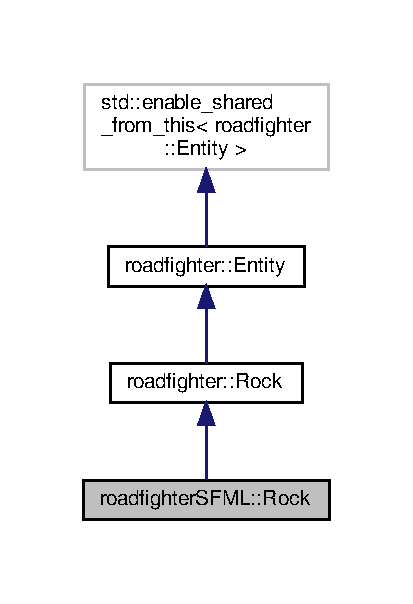
\includegraphics[width=198pt]{classroadfighterSFML_1_1Rock__inherit__graph}
\end{center}
\end{figure}


Collaboration diagram for roadfighter\+S\+F\+ML\+:\+:Rock\+:\nopagebreak
\begin{figure}[H]
\begin{center}
\leavevmode
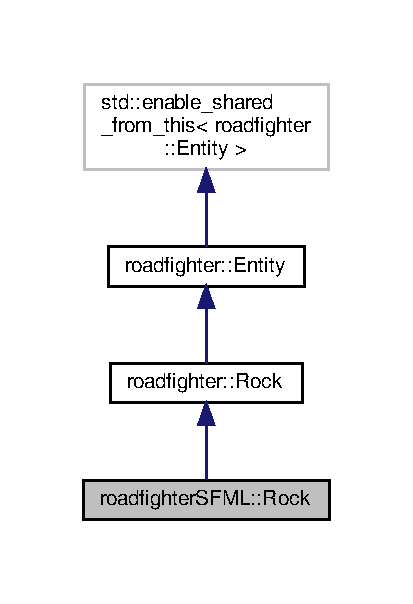
\includegraphics[width=198pt]{classroadfighterSFML_1_1Rock__coll__graph}
\end{center}
\end{figure}
\subsection*{Public Member Functions}
\begin{DoxyCompactItemize}
\item 
void \hyperlink{classroadfighterSFML_1_1Rock_a7416f3e77114d38994d0de4d78e9f403}{draw} () override
\item 
\hyperlink{classroadfighterSFML_1_1Rock_ab3882cc6b5031929881cca55673953a6}{Rock} (std\+::shared\+\_\+ptr$<$ sf\+::\+Render\+Window $>$ window, double i, std\+::shared\+\_\+ptr$<$ \hyperlink{classConfigData}{Config\+Data} $>$ config)
\end{DoxyCompactItemize}
\subsection*{Additional Inherited Members}


\subsection{Detailed Description}
Graphic side of the rock class 

\subsection{Constructor \& Destructor Documentation}
\mbox{\Hypertarget{classroadfighterSFML_1_1Rock_ab3882cc6b5031929881cca55673953a6}\label{classroadfighterSFML_1_1Rock_ab3882cc6b5031929881cca55673953a6}} 
\index{roadfighter\+S\+F\+M\+L\+::\+Rock@{roadfighter\+S\+F\+M\+L\+::\+Rock}!Rock@{Rock}}
\index{Rock@{Rock}!roadfighter\+S\+F\+M\+L\+::\+Rock@{roadfighter\+S\+F\+M\+L\+::\+Rock}}
\subsubsection{\texorpdfstring{Rock()}{Rock()}}
{\footnotesize\ttfamily roadfighter\+S\+F\+M\+L\+::\+Rock\+::\+Rock (\begin{DoxyParamCaption}\item[{std\+::shared\+\_\+ptr$<$ sf\+::\+Render\+Window $>$}]{window,  }\item[{double}]{i,  }\item[{std\+::shared\+\_\+ptr$<$ \hyperlink{classConfigData}{Config\+Data} $>$}]{config }\end{DoxyParamCaption})}

Constructor with sfml window, random position and configuration data 
\begin{DoxyParams}{Parameters}
{\em window} & \\
\hline
{\em i} & \\
\hline
{\em config} & \\
\hline
\end{DoxyParams}


\subsection{Member Function Documentation}
\mbox{\Hypertarget{classroadfighterSFML_1_1Rock_a7416f3e77114d38994d0de4d78e9f403}\label{classroadfighterSFML_1_1Rock_a7416f3e77114d38994d0de4d78e9f403}} 
\index{roadfighter\+S\+F\+M\+L\+::\+Rock@{roadfighter\+S\+F\+M\+L\+::\+Rock}!draw@{draw}}
\index{draw@{draw}!roadfighter\+S\+F\+M\+L\+::\+Rock@{roadfighter\+S\+F\+M\+L\+::\+Rock}}
\subsubsection{\texorpdfstring{draw()}{draw()}}
{\footnotesize\ttfamily void roadfighter\+S\+F\+M\+L\+::\+Rock\+::draw (\begin{DoxyParamCaption}{ }\end{DoxyParamCaption})\hspace{0.3cm}{\ttfamily [override]}, {\ttfamily [virtual]}}

draws the object 

Implements \hyperlink{classroadfighter_1_1Entity_ac516f8005f969ad5a86c252e5a3640ee}{roadfighter\+::\+Entity}.



The documentation for this class was generated from the following files\+:\begin{DoxyCompactItemize}
\item 
roadfighter\+S\+F\+M\+L/Rock.\+h\item 
roadfighter\+S\+F\+M\+L/Rock.\+cpp\end{DoxyCompactItemize}

\hypertarget{classroadfighter_1_1Rock}{}\section{roadfighter\+:\+:Rock Class Reference}
\label{classroadfighter_1_1Rock}\index{roadfighter\+::\+Rock@{roadfighter\+::\+Rock}}


{\ttfamily \#include $<$Rock.\+h$>$}



Inheritance diagram for roadfighter\+:\+:Rock\+:\nopagebreak
\begin{figure}[H]
\begin{center}
\leavevmode
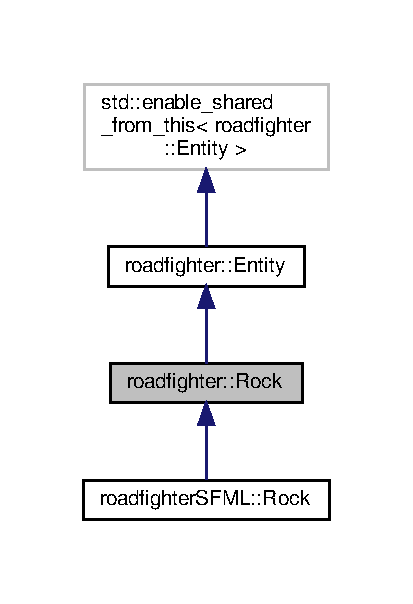
\includegraphics[width=198pt]{classroadfighter_1_1Rock__inherit__graph}
\end{center}
\end{figure}


Collaboration diagram for roadfighter\+:\+:Rock\+:\nopagebreak
\begin{figure}[H]
\begin{center}
\leavevmode
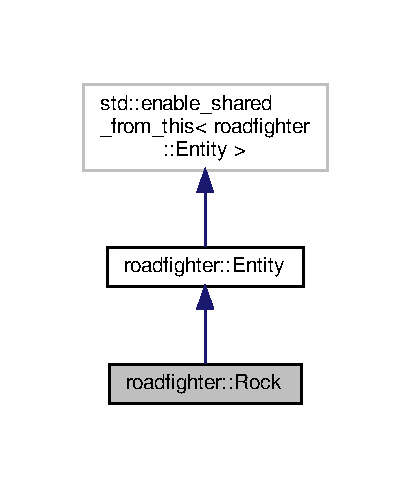
\includegraphics[width=197pt]{classroadfighter_1_1Rock__coll__graph}
\end{center}
\end{figure}
\subsection*{Public Member Functions}
\begin{DoxyCompactItemize}
\item 
void \hyperlink{classroadfighter_1_1Rock_af9817c01175d300ca7be67e2b5e3952e}{update} (int \hyperlink{classroadfighter_1_1Rock_a6e25f8d74c9cba5a22da33bb24518063}{speed}, std\+::shared\+\_\+ptr$<$ \hyperlink{classroadfighter_1_1Entity}{roadfighter\+::\+Entity} $>$ Player) override
\item 
void \hyperlink{classroadfighter_1_1Rock_a28d9c3334f54db88785696076a8b6c9c}{update} () override
\item 
int \hyperlink{classroadfighter_1_1Rock_ab3f596c927c49ab4b159391dc7287192}{get\+Speed} () override
\item 
int \hyperlink{classroadfighter_1_1Rock_a7ac4934b909f1f988b64ac8afc84ea85}{Delete} () override
\item 
void \hyperlink{classroadfighter_1_1Rock_ae2cef1d49610edd8b0438b6c84fdabfd}{set\+Delete} (int del) override
\item 
std\+::shared\+\_\+ptr$<$ \hyperlink{structObjBox}{Obj\+Box} $>$ \hyperlink{classroadfighter_1_1Rock_a286656165c7dd3cdf66945e47f6fa4c7}{get\+Objbox} () override
\item 
bool \hyperlink{classroadfighter_1_1Rock_a1bcf89f9c386a3b248033ba3f0329e9c}{Shoot} () override
\end{DoxyCompactItemize}
\subsection*{Protected Attributes}
\begin{DoxyCompactItemize}
\item 
std\+::pair$<$ double, double $>$ \hyperlink{classroadfighter_1_1Rock_a31327b11d04ef2d368acf12dcffbf21d}{centralpos}
\item 
int \hyperlink{classroadfighter_1_1Rock_a6e25f8d74c9cba5a22da33bb24518063}{speed} = 0
\item 
int \hyperlink{classroadfighter_1_1Rock_a335c9ad9f6931075b34bfa15adf15fa6}{to\+Del} = 0
\item 
double \hyperlink{classroadfighter_1_1Rock_a5551bc7292d6e01a3893128eba4ca4f1}{height}
\item 
double \hyperlink{classroadfighter_1_1Rock_a68752ff27db401333fa3e0e1a504213d}{width}
\end{DoxyCompactItemize}


\subsection{Detailed Description}
The rock obstacle that doesn\textquotesingle{}t have any speed so comes at the player faster 

\subsection{Member Function Documentation}
\mbox{\Hypertarget{classroadfighter_1_1Rock_a7ac4934b909f1f988b64ac8afc84ea85}\label{classroadfighter_1_1Rock_a7ac4934b909f1f988b64ac8afc84ea85}} 
\index{roadfighter\+::\+Rock@{roadfighter\+::\+Rock}!Delete@{Delete}}
\index{Delete@{Delete}!roadfighter\+::\+Rock@{roadfighter\+::\+Rock}}
\subsubsection{\texorpdfstring{Delete()}{Delete()}}
{\footnotesize\ttfamily int roadfighter\+::\+Rock\+::\+Delete (\begin{DoxyParamCaption}{ }\end{DoxyParamCaption})\hspace{0.3cm}{\ttfamily [override]}, {\ttfamily [virtual]}}

Returns a certain value to determine the delete status 0 = nothing, 1 = delete, 2 = respawn \begin{DoxyReturn}{Returns}

\end{DoxyReturn}


Implements \hyperlink{classroadfighter_1_1Entity_a08190b0b8e6a3fcdb42273d6096152ac}{roadfighter\+::\+Entity}.

\mbox{\Hypertarget{classroadfighter_1_1Rock_a286656165c7dd3cdf66945e47f6fa4c7}\label{classroadfighter_1_1Rock_a286656165c7dd3cdf66945e47f6fa4c7}} 
\index{roadfighter\+::\+Rock@{roadfighter\+::\+Rock}!get\+Objbox@{get\+Objbox}}
\index{get\+Objbox@{get\+Objbox}!roadfighter\+::\+Rock@{roadfighter\+::\+Rock}}
\subsubsection{\texorpdfstring{get\+Objbox()}{getObjbox()}}
{\footnotesize\ttfamily std\+::shared\+\_\+ptr$<$ \hyperlink{structObjBox}{Obj\+Box} $>$ roadfighter\+::\+Rock\+::get\+Objbox (\begin{DoxyParamCaption}{ }\end{DoxyParamCaption})\hspace{0.3cm}{\ttfamily [override]}, {\ttfamily [virtual]}}

Return the object box of an object \begin{DoxyReturn}{Returns}

\end{DoxyReturn}


Implements \hyperlink{classroadfighter_1_1Entity_af14340d04a725175a6d221f23c35fa0c}{roadfighter\+::\+Entity}.

\mbox{\Hypertarget{classroadfighter_1_1Rock_ab3f596c927c49ab4b159391dc7287192}\label{classroadfighter_1_1Rock_ab3f596c927c49ab4b159391dc7287192}} 
\index{roadfighter\+::\+Rock@{roadfighter\+::\+Rock}!get\+Speed@{get\+Speed}}
\index{get\+Speed@{get\+Speed}!roadfighter\+::\+Rock@{roadfighter\+::\+Rock}}
\subsubsection{\texorpdfstring{get\+Speed()}{getSpeed()}}
{\footnotesize\ttfamily int roadfighter\+::\+Rock\+::get\+Speed (\begin{DoxyParamCaption}{ }\end{DoxyParamCaption})\hspace{0.3cm}{\ttfamily [override]}, {\ttfamily [virtual]}}

Returns the speed of the object \begin{DoxyReturn}{Returns}
speed 
\end{DoxyReturn}


Implements \hyperlink{classroadfighter_1_1Entity_ad3760184d764a61922e1db7d98501ee4}{roadfighter\+::\+Entity}.

\mbox{\Hypertarget{classroadfighter_1_1Rock_ae2cef1d49610edd8b0438b6c84fdabfd}\label{classroadfighter_1_1Rock_ae2cef1d49610edd8b0438b6c84fdabfd}} 
\index{roadfighter\+::\+Rock@{roadfighter\+::\+Rock}!set\+Delete@{set\+Delete}}
\index{set\+Delete@{set\+Delete}!roadfighter\+::\+Rock@{roadfighter\+::\+Rock}}
\subsubsection{\texorpdfstring{set\+Delete()}{setDelete()}}
{\footnotesize\ttfamily void roadfighter\+::\+Rock\+::set\+Delete (\begin{DoxyParamCaption}\item[{int}]{del }\end{DoxyParamCaption})\hspace{0.3cm}{\ttfamily [override]}, {\ttfamily [virtual]}}

Set if an object must be deleted 
\begin{DoxyParams}{Parameters}
{\em del} & \\
\hline
\end{DoxyParams}


Implements \hyperlink{classroadfighter_1_1Entity_a07e973f0fa941a69e749629716877692}{roadfighter\+::\+Entity}.

\mbox{\Hypertarget{classroadfighter_1_1Rock_a1bcf89f9c386a3b248033ba3f0329e9c}\label{classroadfighter_1_1Rock_a1bcf89f9c386a3b248033ba3f0329e9c}} 
\index{roadfighter\+::\+Rock@{roadfighter\+::\+Rock}!Shoot@{Shoot}}
\index{Shoot@{Shoot}!roadfighter\+::\+Rock@{roadfighter\+::\+Rock}}
\subsubsection{\texorpdfstring{Shoot()}{Shoot()}}
{\footnotesize\ttfamily bool roadfighter\+::\+Rock\+::\+Shoot (\begin{DoxyParamCaption}{ }\end{DoxyParamCaption})\hspace{0.3cm}{\ttfamily [override]}, {\ttfamily [virtual]}}

Return if we have to shoot but this function is only used by the player \begin{DoxyReturn}{Returns}

\end{DoxyReturn}


Implements \hyperlink{classroadfighter_1_1Entity_ad0ecaa0539db252e591da83814251509}{roadfighter\+::\+Entity}.

\mbox{\Hypertarget{classroadfighter_1_1Rock_af9817c01175d300ca7be67e2b5e3952e}\label{classroadfighter_1_1Rock_af9817c01175d300ca7be67e2b5e3952e}} 
\index{roadfighter\+::\+Rock@{roadfighter\+::\+Rock}!update@{update}}
\index{update@{update}!roadfighter\+::\+Rock@{roadfighter\+::\+Rock}}
\subsubsection{\texorpdfstring{update()}{update()}\hspace{0.1cm}{\footnotesize\ttfamily [1/2]}}
{\footnotesize\ttfamily void roadfighter\+::\+Rock\+::update (\begin{DoxyParamCaption}\item[{int}]{speed,  }\item[{std\+::shared\+\_\+ptr$<$ \hyperlink{classroadfighter_1_1Entity}{roadfighter\+::\+Entity} $>$}]{Player }\end{DoxyParamCaption})\hspace{0.3cm}{\ttfamily [override]}, {\ttfamily [virtual]}}

Updates the object with extra parameters 
\begin{DoxyParams}{Parameters}
{\em speed} & \\
\hline
{\em Player} & \\
\hline
\end{DoxyParams}


Implements \hyperlink{classroadfighter_1_1Entity_a611ba56595dd2137d308876ba820cc09}{roadfighter\+::\+Entity}.

\mbox{\Hypertarget{classroadfighter_1_1Rock_a28d9c3334f54db88785696076a8b6c9c}\label{classroadfighter_1_1Rock_a28d9c3334f54db88785696076a8b6c9c}} 
\index{roadfighter\+::\+Rock@{roadfighter\+::\+Rock}!update@{update}}
\index{update@{update}!roadfighter\+::\+Rock@{roadfighter\+::\+Rock}}
\subsubsection{\texorpdfstring{update()}{update()}\hspace{0.1cm}{\footnotesize\ttfamily [2/2]}}
{\footnotesize\ttfamily void roadfighter\+::\+Rock\+::update (\begin{DoxyParamCaption}{ }\end{DoxyParamCaption})\hspace{0.3cm}{\ttfamily [override]}, {\ttfamily [virtual]}}

Update the object 

Implements \hyperlink{classroadfighter_1_1Entity_a19cd353f12a3e8432acd6d5609137561}{roadfighter\+::\+Entity}.



\subsection{Member Data Documentation}
\mbox{\Hypertarget{classroadfighter_1_1Rock_a31327b11d04ef2d368acf12dcffbf21d}\label{classroadfighter_1_1Rock_a31327b11d04ef2d368acf12dcffbf21d}} 
\index{roadfighter\+::\+Rock@{roadfighter\+::\+Rock}!centralpos@{centralpos}}
\index{centralpos@{centralpos}!roadfighter\+::\+Rock@{roadfighter\+::\+Rock}}
\subsubsection{\texorpdfstring{centralpos}{centralpos}}
{\footnotesize\ttfamily std\+::pair$<$double, double$>$ roadfighter\+::\+Rock\+::centralpos\hspace{0.3cm}{\ttfamily [protected]}}

Pair of the doubles that contains the x and y position of the center of the object \mbox{\Hypertarget{classroadfighter_1_1Rock_a5551bc7292d6e01a3893128eba4ca4f1}\label{classroadfighter_1_1Rock_a5551bc7292d6e01a3893128eba4ca4f1}} 
\index{roadfighter\+::\+Rock@{roadfighter\+::\+Rock}!height@{height}}
\index{height@{height}!roadfighter\+::\+Rock@{roadfighter\+::\+Rock}}
\subsubsection{\texorpdfstring{height}{height}}
{\footnotesize\ttfamily double roadfighter\+::\+Rock\+::height\hspace{0.3cm}{\ttfamily [protected]}}

Height of object \mbox{\Hypertarget{classroadfighter_1_1Rock_a6e25f8d74c9cba5a22da33bb24518063}\label{classroadfighter_1_1Rock_a6e25f8d74c9cba5a22da33bb24518063}} 
\index{roadfighter\+::\+Rock@{roadfighter\+::\+Rock}!speed@{speed}}
\index{speed@{speed}!roadfighter\+::\+Rock@{roadfighter\+::\+Rock}}
\subsubsection{\texorpdfstring{speed}{speed}}
{\footnotesize\ttfamily int roadfighter\+::\+Rock\+::speed = 0\hspace{0.3cm}{\ttfamily [protected]}}

Speed of the object \mbox{\Hypertarget{classroadfighter_1_1Rock_a335c9ad9f6931075b34bfa15adf15fa6}\label{classroadfighter_1_1Rock_a335c9ad9f6931075b34bfa15adf15fa6}} 
\index{roadfighter\+::\+Rock@{roadfighter\+::\+Rock}!to\+Del@{to\+Del}}
\index{to\+Del@{to\+Del}!roadfighter\+::\+Rock@{roadfighter\+::\+Rock}}
\subsubsection{\texorpdfstring{to\+Del}{toDel}}
{\footnotesize\ttfamily int roadfighter\+::\+Rock\+::to\+Del = 0\hspace{0.3cm}{\ttfamily [protected]}}

Object deletion status ( 0 = nothing, 1 = delete, 2 = respawn ) \mbox{\Hypertarget{classroadfighter_1_1Rock_a68752ff27db401333fa3e0e1a504213d}\label{classroadfighter_1_1Rock_a68752ff27db401333fa3e0e1a504213d}} 
\index{roadfighter\+::\+Rock@{roadfighter\+::\+Rock}!width@{width}}
\index{width@{width}!roadfighter\+::\+Rock@{roadfighter\+::\+Rock}}
\subsubsection{\texorpdfstring{width}{width}}
{\footnotesize\ttfamily double roadfighter\+::\+Rock\+::width\hspace{0.3cm}{\ttfamily [protected]}}

Width of object 

The documentation for this class was generated from the following files\+:\begin{DoxyCompactItemize}
\item 
roadfighter/Rock.\+h\item 
roadfighter/Rock.\+cpp\end{DoxyCompactItemize}

\hypertarget{classScoreboard}{}\section{Scoreboard Class Reference}
\label{classScoreboard}\index{Scoreboard@{Scoreboard}}


{\ttfamily \#include $<$Scoreboard.\+h$>$}

\subsection*{Public Member Functions}
\begin{DoxyCompactItemize}
\item 
\hyperlink{classScoreboard_ae3b3273b61018b83bf72a18649de706f}{Scoreboard} (std\+::shared\+\_\+ptr$<$ sf\+::\+Render\+Window $>$ window, std\+::shared\+\_\+ptr$<$ \hyperlink{classConfigData}{Config\+Data} $>$ config)
\item 
void \hyperlink{classScoreboard_ae12729e1ea694e1ec2d8651a10c582b1}{draw\+Board} ()
\item 
void \hyperlink{classScoreboard_aa968340a9217f6ccd2ef4da7e43303b5}{set\+Scores\+Current\+Game} (const std\+::vector$<$ int $>$ \&scores\+Current\+Game)
\end{DoxyCompactItemize}


\subsection{Detailed Description}
Handles the scoreboard at the end of the game 

\subsection{Constructor \& Destructor Documentation}
\mbox{\Hypertarget{classScoreboard_ae3b3273b61018b83bf72a18649de706f}\label{classScoreboard_ae3b3273b61018b83bf72a18649de706f}} 
\index{Scoreboard@{Scoreboard}!Scoreboard@{Scoreboard}}
\index{Scoreboard@{Scoreboard}!Scoreboard@{Scoreboard}}
\subsubsection{\texorpdfstring{Scoreboard()}{Scoreboard()}}
{\footnotesize\ttfamily Scoreboard\+::\+Scoreboard (\begin{DoxyParamCaption}\item[{std\+::shared\+\_\+ptr$<$ sf\+::\+Render\+Window $>$}]{window,  }\item[{std\+::shared\+\_\+ptr$<$ \hyperlink{classConfigData}{Config\+Data} $>$}]{config }\end{DoxyParamCaption})}

Constructor with sfml window and configuration data 
\begin{DoxyParams}{Parameters}
{\em window} & \\
\hline
{\em config} & \\
\hline
\end{DoxyParams}


\subsection{Member Function Documentation}
\mbox{\Hypertarget{classScoreboard_ae12729e1ea694e1ec2d8651a10c582b1}\label{classScoreboard_ae12729e1ea694e1ec2d8651a10c582b1}} 
\index{Scoreboard@{Scoreboard}!draw\+Board@{draw\+Board}}
\index{draw\+Board@{draw\+Board}!Scoreboard@{Scoreboard}}
\subsubsection{\texorpdfstring{draw\+Board()}{drawBoard()}}
{\footnotesize\ttfamily void Scoreboard\+::draw\+Board (\begin{DoxyParamCaption}{ }\end{DoxyParamCaption})}

Drawing the scoreboard with the scores specified in the highscore file \mbox{\Hypertarget{classScoreboard_aa968340a9217f6ccd2ef4da7e43303b5}\label{classScoreboard_aa968340a9217f6ccd2ef4da7e43303b5}} 
\index{Scoreboard@{Scoreboard}!set\+Scores\+Current\+Game@{set\+Scores\+Current\+Game}}
\index{set\+Scores\+Current\+Game@{set\+Scores\+Current\+Game}!Scoreboard@{Scoreboard}}
\subsubsection{\texorpdfstring{set\+Scores\+Current\+Game()}{setScoresCurrentGame()}}
{\footnotesize\ttfamily void Scoreboard\+::set\+Scores\+Current\+Game (\begin{DoxyParamCaption}\item[{const std\+::vector$<$ int $>$ \&}]{scores\+Current\+Game }\end{DoxyParamCaption})}

Calculate the total score of the current game and updates the highscore file correspondingly 
\begin{DoxyParams}{Parameters}
{\em scores\+Current\+Game} & \\
\hline
\end{DoxyParams}


The documentation for this class was generated from the following files\+:\begin{DoxyCompactItemize}
\item 
Scoreboard.\+h\item 
Scoreboard.\+cpp\end{DoxyCompactItemize}

\hypertarget{classScoreError}{}\section{Score\+Error Class Reference}
\label{classScoreError}\index{Score\+Error@{Score\+Error}}


{\ttfamily \#include $<$Score\+Error.\+h$>$}



Inheritance diagram for Score\+Error\+:\nopagebreak
\begin{figure}[H]
\begin{center}
\leavevmode
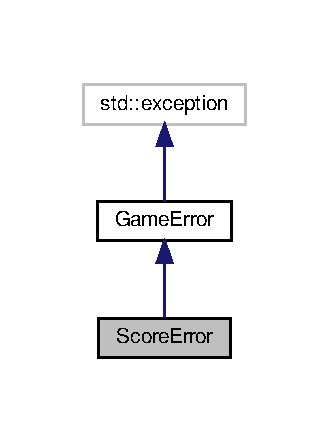
\includegraphics[width=158pt]{classScoreError__inherit__graph}
\end{center}
\end{figure}


Collaboration diagram for Score\+Error\+:\nopagebreak
\begin{figure}[H]
\begin{center}
\leavevmode
\includegraphics[width=158pt]{classScoreError__coll__graph}
\end{center}
\end{figure}
\subsection*{Public Member Functions}
\begin{DoxyCompactItemize}
\item 
const char $\ast$ \hyperlink{classScoreError_a56e2018c9c0c9d34b482533aa983d37d}{what} () const noexcept override
\end{DoxyCompactItemize}


\subsection{Detailed Description}
Error that appears when there is a fault with the score 

\subsection{Member Function Documentation}
\mbox{\Hypertarget{classScoreError_a56e2018c9c0c9d34b482533aa983d37d}\label{classScoreError_a56e2018c9c0c9d34b482533aa983d37d}} 
\index{Score\+Error@{Score\+Error}!what@{what}}
\index{what@{what}!Score\+Error@{Score\+Error}}
\subsubsection{\texorpdfstring{what()}{what()}}
{\footnotesize\ttfamily const char $\ast$ Score\+Error\+::what (\begin{DoxyParamCaption}{ }\end{DoxyParamCaption}) const\hspace{0.3cm}{\ttfamily [override]}, {\ttfamily [virtual]}, {\ttfamily [noexcept]}}

Return the error message \begin{DoxyReturn}{Returns}

\end{DoxyReturn}


Implements \hyperlink{classGameError_afbe93d6a2023f2824be2733aff9e86cb}{Game\+Error}.



The documentation for this class was generated from the following files\+:\begin{DoxyCompactItemize}
\item 
Exception\+\_\+class/Score\+Error.\+h\item 
Exception\+\_\+class/Score\+Error.\+cpp\end{DoxyCompactItemize}

\hypertarget{classroadfighterSFML_1_1SFMLFactory}{}\section{roadfighter\+S\+F\+ML\+:\+:S\+F\+M\+L\+Factory Class Reference}
\label{classroadfighterSFML_1_1SFMLFactory}\index{roadfighter\+S\+F\+M\+L\+::\+S\+F\+M\+L\+Factory@{roadfighter\+S\+F\+M\+L\+::\+S\+F\+M\+L\+Factory}}


{\ttfamily \#include $<$S\+F\+M\+L\+Factory.\+h$>$}



Inheritance diagram for roadfighter\+S\+F\+ML\+:\+:S\+F\+M\+L\+Factory\+:\nopagebreak
\begin{figure}[H]
\begin{center}
\leavevmode
\includegraphics[width=234pt]{classroadfighterSFML_1_1SFMLFactory__inherit__graph}
\end{center}
\end{figure}


Collaboration diagram for roadfighter\+S\+F\+ML\+:\+:S\+F\+M\+L\+Factory\+:\nopagebreak
\begin{figure}[H]
\begin{center}
\leavevmode
\includegraphics[width=234pt]{classroadfighterSFML_1_1SFMLFactory__coll__graph}
\end{center}
\end{figure}
\subsection*{Public Member Functions}
\begin{DoxyCompactItemize}
\item 
\hyperlink{classroadfighterSFML_1_1SFMLFactory_af39bfa15dc13886b0fa9096baa273377}{S\+F\+M\+L\+Factory} (std\+::shared\+\_\+ptr$<$ sf\+::\+Render\+Window $>$ window, std\+::shared\+\_\+ptr$<$ \hyperlink{classConfigData}{Config\+Data} $>$ Config)
\item 
std\+::shared\+\_\+ptr$<$ \hyperlink{classroadfighter_1_1Entity}{roadfighter\+::\+Entity} $>$ \hyperlink{classroadfighterSFML_1_1SFMLFactory_acb966ae41ef0a928c4adc34b4c97cedb}{create\+Player\+Car} (int level) override
\item 
std\+::shared\+\_\+ptr$<$ \hyperlink{classroadfighter_1_1Entity}{roadfighter\+::\+Entity} $>$ \hyperlink{classroadfighterSFML_1_1SFMLFactory_a18a78a7113edf49647f727105329f605}{create\+Background} (int i) override
\item 
std\+::shared\+\_\+ptr$<$ \hyperlink{classroadfighter_1_1Entity}{roadfighter\+::\+Entity} $>$ \hyperlink{classroadfighterSFML_1_1SFMLFactory_a9960aec21f58babf83857cc400dad8fe}{create\+Passing\+Car} (double i) override
\item 
std\+::shared\+\_\+ptr$<$ \hyperlink{classroadfighter_1_1Entity}{roadfighter\+::\+Entity} $>$ \hyperlink{classroadfighterSFML_1_1SFMLFactory_aac2ed62453b201da7d124947b6cd475b}{create\+Bullet} (double first, double second) override
\item 
std\+::shared\+\_\+ptr$<$ \hyperlink{classroadfighter_1_1Entity}{roadfighter\+::\+Entity} $>$ \hyperlink{classroadfighterSFML_1_1SFMLFactory_ace05bdfcf9fc4f1ca7b9fc6f840b7a12}{create\+Rock} (double i) override
\item 
std\+::shared\+\_\+ptr$<$ \hyperlink{classroadfighter_1_1Entity}{roadfighter\+::\+Entity} $>$ \hyperlink{classroadfighterSFML_1_1SFMLFactory_aa1aeba2d2613b784d9da5f6fd3109154}{create\+Moving\+Car} (double i) override
\item 
std\+::shared\+\_\+ptr$<$ \hyperlink{classroadfighter_1_1AIRacer}{roadfighter\+::\+A\+I\+Racer} $>$ \hyperlink{classroadfighterSFML_1_1SFMLFactory_a977a002d878172e485bea8679c136d76}{create\+AI} () override
\item 
std\+::shared\+\_\+ptr$<$ \hyperlink{classroadfighter_1_1Boss}{roadfighter\+::\+Boss} $>$ \hyperlink{classroadfighterSFML_1_1SFMLFactory_a86f4fed282eebc1556ed1134e7ad7e13}{create\+Boss} () override
\end{DoxyCompactItemize}


\subsection{Detailed Description}
S\+F\+ML side of the factory that makes sure every object can acces the window 

\subsection{Constructor \& Destructor Documentation}
\mbox{\Hypertarget{classroadfighterSFML_1_1SFMLFactory_af39bfa15dc13886b0fa9096baa273377}\label{classroadfighterSFML_1_1SFMLFactory_af39bfa15dc13886b0fa9096baa273377}} 
\index{roadfighter\+S\+F\+M\+L\+::\+S\+F\+M\+L\+Factory@{roadfighter\+S\+F\+M\+L\+::\+S\+F\+M\+L\+Factory}!S\+F\+M\+L\+Factory@{S\+F\+M\+L\+Factory}}
\index{S\+F\+M\+L\+Factory@{S\+F\+M\+L\+Factory}!roadfighter\+S\+F\+M\+L\+::\+S\+F\+M\+L\+Factory@{roadfighter\+S\+F\+M\+L\+::\+S\+F\+M\+L\+Factory}}
\subsubsection{\texorpdfstring{S\+F\+M\+L\+Factory()}{SFMLFactory()}}
{\footnotesize\ttfamily roadfighter\+S\+F\+M\+L\+::\+S\+F\+M\+L\+Factory\+::\+S\+F\+M\+L\+Factory (\begin{DoxyParamCaption}\item[{std\+::shared\+\_\+ptr$<$ sf\+::\+Render\+Window $>$}]{window,  }\item[{std\+::shared\+\_\+ptr$<$ \hyperlink{classConfigData}{Config\+Data} $>$}]{Config }\end{DoxyParamCaption})}

Constructor of factory with sfml window and configuration data 
\begin{DoxyParams}{Parameters}
{\em window} & \\
\hline
{\em Config} & \\
\hline
\end{DoxyParams}


\subsection{Member Function Documentation}
\mbox{\Hypertarget{classroadfighterSFML_1_1SFMLFactory_a977a002d878172e485bea8679c136d76}\label{classroadfighterSFML_1_1SFMLFactory_a977a002d878172e485bea8679c136d76}} 
\index{roadfighter\+S\+F\+M\+L\+::\+S\+F\+M\+L\+Factory@{roadfighter\+S\+F\+M\+L\+::\+S\+F\+M\+L\+Factory}!create\+AI@{create\+AI}}
\index{create\+AI@{create\+AI}!roadfighter\+S\+F\+M\+L\+::\+S\+F\+M\+L\+Factory@{roadfighter\+S\+F\+M\+L\+::\+S\+F\+M\+L\+Factory}}
\subsubsection{\texorpdfstring{create\+A\+I()}{createAI()}}
{\footnotesize\ttfamily std\+::shared\+\_\+ptr$<$ \hyperlink{classroadfighter_1_1AIRacer}{roadfighter\+::\+A\+I\+Racer} $>$ roadfighter\+S\+F\+M\+L\+::\+S\+F\+M\+L\+Factory\+::create\+AI (\begin{DoxyParamCaption}{ }\end{DoxyParamCaption})\hspace{0.3cm}{\ttfamily [override]}, {\ttfamily [virtual]}}

Create an ai \begin{DoxyReturn}{Returns}
shared\+\_\+ptr of Entity 
\end{DoxyReturn}


Implements \hyperlink{classroadfighter_1_1EntityFactory_ae50d1b8cbf0b63dfbedca775781fbda0}{roadfighter\+::\+Entity\+Factory}.

\mbox{\Hypertarget{classroadfighterSFML_1_1SFMLFactory_a18a78a7113edf49647f727105329f605}\label{classroadfighterSFML_1_1SFMLFactory_a18a78a7113edf49647f727105329f605}} 
\index{roadfighter\+S\+F\+M\+L\+::\+S\+F\+M\+L\+Factory@{roadfighter\+S\+F\+M\+L\+::\+S\+F\+M\+L\+Factory}!create\+Background@{create\+Background}}
\index{create\+Background@{create\+Background}!roadfighter\+S\+F\+M\+L\+::\+S\+F\+M\+L\+Factory@{roadfighter\+S\+F\+M\+L\+::\+S\+F\+M\+L\+Factory}}
\subsubsection{\texorpdfstring{create\+Background()}{createBackground()}}
{\footnotesize\ttfamily std\+::shared\+\_\+ptr$<$ \hyperlink{classroadfighter_1_1Entity}{roadfighter\+::\+Entity} $>$ roadfighter\+S\+F\+M\+L\+::\+S\+F\+M\+L\+Factory\+::create\+Background (\begin{DoxyParamCaption}\item[{int}]{i }\end{DoxyParamCaption})\hspace{0.3cm}{\ttfamily [override]}, {\ttfamily [virtual]}}

Create a background \begin{DoxyReturn}{Returns}
shared\+\_\+ptr of Entity 
\end{DoxyReturn}


Implements \hyperlink{classroadfighter_1_1EntityFactory_ab3586917a6ef9d3a92b825f908132e02}{roadfighter\+::\+Entity\+Factory}.

\mbox{\Hypertarget{classroadfighterSFML_1_1SFMLFactory_a86f4fed282eebc1556ed1134e7ad7e13}\label{classroadfighterSFML_1_1SFMLFactory_a86f4fed282eebc1556ed1134e7ad7e13}} 
\index{roadfighter\+S\+F\+M\+L\+::\+S\+F\+M\+L\+Factory@{roadfighter\+S\+F\+M\+L\+::\+S\+F\+M\+L\+Factory}!create\+Boss@{create\+Boss}}
\index{create\+Boss@{create\+Boss}!roadfighter\+S\+F\+M\+L\+::\+S\+F\+M\+L\+Factory@{roadfighter\+S\+F\+M\+L\+::\+S\+F\+M\+L\+Factory}}
\subsubsection{\texorpdfstring{create\+Boss()}{createBoss()}}
{\footnotesize\ttfamily std\+::shared\+\_\+ptr$<$ \hyperlink{classroadfighter_1_1Boss}{roadfighter\+::\+Boss} $>$ roadfighter\+S\+F\+M\+L\+::\+S\+F\+M\+L\+Factory\+::create\+Boss (\begin{DoxyParamCaption}{ }\end{DoxyParamCaption})\hspace{0.3cm}{\ttfamily [override]}, {\ttfamily [virtual]}}

Create a boss \begin{DoxyReturn}{Returns}
shared\+\_\+ptr of Entity 
\end{DoxyReturn}


Implements \hyperlink{classroadfighter_1_1EntityFactory_ae7a09423660432e744ed35f5f04b0931}{roadfighter\+::\+Entity\+Factory}.

\mbox{\Hypertarget{classroadfighterSFML_1_1SFMLFactory_aac2ed62453b201da7d124947b6cd475b}\label{classroadfighterSFML_1_1SFMLFactory_aac2ed62453b201da7d124947b6cd475b}} 
\index{roadfighter\+S\+F\+M\+L\+::\+S\+F\+M\+L\+Factory@{roadfighter\+S\+F\+M\+L\+::\+S\+F\+M\+L\+Factory}!create\+Bullet@{create\+Bullet}}
\index{create\+Bullet@{create\+Bullet}!roadfighter\+S\+F\+M\+L\+::\+S\+F\+M\+L\+Factory@{roadfighter\+S\+F\+M\+L\+::\+S\+F\+M\+L\+Factory}}
\subsubsection{\texorpdfstring{create\+Bullet()}{createBullet()}}
{\footnotesize\ttfamily std\+::shared\+\_\+ptr$<$ \hyperlink{classroadfighter_1_1Entity}{roadfighter\+::\+Entity} $>$ roadfighter\+S\+F\+M\+L\+::\+S\+F\+M\+L\+Factory\+::create\+Bullet (\begin{DoxyParamCaption}\item[{double}]{first,  }\item[{double}]{second }\end{DoxyParamCaption})\hspace{0.3cm}{\ttfamily [override]}, {\ttfamily [virtual]}}

Create a \hyperlink{classroadfighterSFML_1_1Bullet}{Bullet} with to doubles for the location of the car 
\begin{DoxyParams}{Parameters}
{\em first} & = x location \\
\hline
{\em second} & = y location \\
\hline
\end{DoxyParams}
\begin{DoxyReturn}{Returns}
shared\+\_\+ptr of Entity 
\end{DoxyReturn}


Implements \hyperlink{classroadfighter_1_1EntityFactory_a2d4319aef20024f83e7c3189e92c89e1}{roadfighter\+::\+Entity\+Factory}.

\mbox{\Hypertarget{classroadfighterSFML_1_1SFMLFactory_aa1aeba2d2613b784d9da5f6fd3109154}\label{classroadfighterSFML_1_1SFMLFactory_aa1aeba2d2613b784d9da5f6fd3109154}} 
\index{roadfighter\+S\+F\+M\+L\+::\+S\+F\+M\+L\+Factory@{roadfighter\+S\+F\+M\+L\+::\+S\+F\+M\+L\+Factory}!create\+Moving\+Car@{create\+Moving\+Car}}
\index{create\+Moving\+Car@{create\+Moving\+Car}!roadfighter\+S\+F\+M\+L\+::\+S\+F\+M\+L\+Factory@{roadfighter\+S\+F\+M\+L\+::\+S\+F\+M\+L\+Factory}}
\subsubsection{\texorpdfstring{create\+Moving\+Car()}{createMovingCar()}}
{\footnotesize\ttfamily std\+::shared\+\_\+ptr$<$ \hyperlink{classroadfighter_1_1Entity}{roadfighter\+::\+Entity} $>$ roadfighter\+S\+F\+M\+L\+::\+S\+F\+M\+L\+Factory\+::create\+Moving\+Car (\begin{DoxyParamCaption}\item[{double}]{i }\end{DoxyParamCaption})\hspace{0.3cm}{\ttfamily [override]}, {\ttfamily [virtual]}}

Create a moving car with a random position 
\begin{DoxyParams}{Parameters}
{\em i} & \\
\hline
\end{DoxyParams}
\begin{DoxyReturn}{Returns}
shared\+\_\+ptr of Entity 
\end{DoxyReturn}


Implements \hyperlink{classroadfighter_1_1EntityFactory_a53cc68cc3f7365e4ded258ea9b281b45}{roadfighter\+::\+Entity\+Factory}.

\mbox{\Hypertarget{classroadfighterSFML_1_1SFMLFactory_a9960aec21f58babf83857cc400dad8fe}\label{classroadfighterSFML_1_1SFMLFactory_a9960aec21f58babf83857cc400dad8fe}} 
\index{roadfighter\+S\+F\+M\+L\+::\+S\+F\+M\+L\+Factory@{roadfighter\+S\+F\+M\+L\+::\+S\+F\+M\+L\+Factory}!create\+Passing\+Car@{create\+Passing\+Car}}
\index{create\+Passing\+Car@{create\+Passing\+Car}!roadfighter\+S\+F\+M\+L\+::\+S\+F\+M\+L\+Factory@{roadfighter\+S\+F\+M\+L\+::\+S\+F\+M\+L\+Factory}}
\subsubsection{\texorpdfstring{create\+Passing\+Car()}{createPassingCar()}}
{\footnotesize\ttfamily std\+::shared\+\_\+ptr$<$ \hyperlink{classroadfighter_1_1Entity}{roadfighter\+::\+Entity} $>$ roadfighter\+S\+F\+M\+L\+::\+S\+F\+M\+L\+Factory\+::create\+Passing\+Car (\begin{DoxyParamCaption}\item[{double}]{i }\end{DoxyParamCaption})\hspace{0.3cm}{\ttfamily [override]}, {\ttfamily [virtual]}}

Create a passing car 
\begin{DoxyParams}{Parameters}
{\em i} & = random value to spawn \\
\hline
\end{DoxyParams}
\begin{DoxyReturn}{Returns}
shared\+\_\+ptr of Entity 
\end{DoxyReturn}


Implements \hyperlink{classroadfighter_1_1EntityFactory_ab318794f4effc0c2195fae5da267d900}{roadfighter\+::\+Entity\+Factory}.

\mbox{\Hypertarget{classroadfighterSFML_1_1SFMLFactory_acb966ae41ef0a928c4adc34b4c97cedb}\label{classroadfighterSFML_1_1SFMLFactory_acb966ae41ef0a928c4adc34b4c97cedb}} 
\index{roadfighter\+S\+F\+M\+L\+::\+S\+F\+M\+L\+Factory@{roadfighter\+S\+F\+M\+L\+::\+S\+F\+M\+L\+Factory}!create\+Player\+Car@{create\+Player\+Car}}
\index{create\+Player\+Car@{create\+Player\+Car}!roadfighter\+S\+F\+M\+L\+::\+S\+F\+M\+L\+Factory@{roadfighter\+S\+F\+M\+L\+::\+S\+F\+M\+L\+Factory}}
\subsubsection{\texorpdfstring{create\+Player\+Car()}{createPlayerCar()}}
{\footnotesize\ttfamily std\+::shared\+\_\+ptr$<$ \hyperlink{classroadfighter_1_1Entity}{roadfighter\+::\+Entity} $>$ roadfighter\+S\+F\+M\+L\+::\+S\+F\+M\+L\+Factory\+::create\+Player\+Car (\begin{DoxyParamCaption}\item[{int}]{level }\end{DoxyParamCaption})\hspace{0.3cm}{\ttfamily [override]}, {\ttfamily [virtual]}}

Create a playercar \begin{DoxyReturn}{Returns}
shared\+\_\+ptr of Entity 
\end{DoxyReturn}


Implements \hyperlink{classroadfighter_1_1EntityFactory_a8fefd94a197c87544805461761fc111c}{roadfighter\+::\+Entity\+Factory}.

\mbox{\Hypertarget{classroadfighterSFML_1_1SFMLFactory_ace05bdfcf9fc4f1ca7b9fc6f840b7a12}\label{classroadfighterSFML_1_1SFMLFactory_ace05bdfcf9fc4f1ca7b9fc6f840b7a12}} 
\index{roadfighter\+S\+F\+M\+L\+::\+S\+F\+M\+L\+Factory@{roadfighter\+S\+F\+M\+L\+::\+S\+F\+M\+L\+Factory}!create\+Rock@{create\+Rock}}
\index{create\+Rock@{create\+Rock}!roadfighter\+S\+F\+M\+L\+::\+S\+F\+M\+L\+Factory@{roadfighter\+S\+F\+M\+L\+::\+S\+F\+M\+L\+Factory}}
\subsubsection{\texorpdfstring{create\+Rock()}{createRock()}}
{\footnotesize\ttfamily std\+::shared\+\_\+ptr$<$ \hyperlink{classroadfighter_1_1Entity}{roadfighter\+::\+Entity} $>$ roadfighter\+S\+F\+M\+L\+::\+S\+F\+M\+L\+Factory\+::create\+Rock (\begin{DoxyParamCaption}\item[{double}]{i }\end{DoxyParamCaption})\hspace{0.3cm}{\ttfamily [override]}, {\ttfamily [virtual]}}

Create a \hyperlink{classroadfighterSFML_1_1Rock}{Rock} with a random position 
\begin{DoxyParams}{Parameters}
{\em i} & \\
\hline
\end{DoxyParams}
\begin{DoxyReturn}{Returns}
shared\+\_\+ptr of Entity 
\end{DoxyReturn}


Implements \hyperlink{classroadfighter_1_1EntityFactory_a3bcb7e8b8ca62628c842962cfbba50be}{roadfighter\+::\+Entity\+Factory}.



The documentation for this class was generated from the following files\+:\begin{DoxyCompactItemize}
\item 
roadfighter\+S\+F\+M\+L/S\+F\+M\+L\+Factory.\+h\item 
roadfighter\+S\+F\+M\+L/S\+F\+M\+L\+Factory.\+cpp\end{DoxyCompactItemize}

\hypertarget{classSpriteLoadError}{}\section{Sprite\+Load\+Error Class Reference}
\label{classSpriteLoadError}\index{Sprite\+Load\+Error@{Sprite\+Load\+Error}}


{\ttfamily \#include $<$Sprite\+Load\+Error.\+h$>$}



Inheritance diagram for Sprite\+Load\+Error\+:\nopagebreak
\begin{figure}[H]
\begin{center}
\leavevmode
\includegraphics[width=164pt]{classSpriteLoadError__inherit__graph}
\end{center}
\end{figure}


Collaboration diagram for Sprite\+Load\+Error\+:\nopagebreak
\begin{figure}[H]
\begin{center}
\leavevmode
\includegraphics[width=164pt]{classSpriteLoadError__coll__graph}
\end{center}
\end{figure}
\subsection*{Public Member Functions}
\begin{DoxyCompactItemize}
\item 
\hyperlink{classSpriteLoadError_a28b49ab4f2fb92283d272c25a3582994}{Sprite\+Load\+Error} (const char $\ast$\hyperlink{classFileError_a0ea1cc225bf7f8fa47aa0cfa0c2ba685}{file})
\item 
const char $\ast$ \hyperlink{classSpriteLoadError_a7b51c2ea656c91b352514cd77aab0a38}{what} () const noexcept override
\item 
const char $\ast$ \hyperlink{classSpriteLoadError_aa6c6ca97b781b8045eb4271aad6aa6d1}{file\+Path} () const noexcept override
\end{DoxyCompactItemize}
\subsection*{Additional Inherited Members}


\subsection{Detailed Description}
Error that appears when failing to load a sprite 

\subsection{Constructor \& Destructor Documentation}
\mbox{\Hypertarget{classSpriteLoadError_a28b49ab4f2fb92283d272c25a3582994}\label{classSpriteLoadError_a28b49ab4f2fb92283d272c25a3582994}} 
\index{Sprite\+Load\+Error@{Sprite\+Load\+Error}!Sprite\+Load\+Error@{Sprite\+Load\+Error}}
\index{Sprite\+Load\+Error@{Sprite\+Load\+Error}!Sprite\+Load\+Error@{Sprite\+Load\+Error}}
\subsubsection{\texorpdfstring{Sprite\+Load\+Error()}{SpriteLoadError()}}
{\footnotesize\ttfamily Sprite\+Load\+Error\+::\+Sprite\+Load\+Error (\begin{DoxyParamCaption}\item[{const char $\ast$}]{file }\end{DoxyParamCaption})}

Constructor with the file that caused the error 
\begin{DoxyParams}{Parameters}
{\em file} & \\
\hline
\end{DoxyParams}


\subsection{Member Function Documentation}
\mbox{\Hypertarget{classSpriteLoadError_aa6c6ca97b781b8045eb4271aad6aa6d1}\label{classSpriteLoadError_aa6c6ca97b781b8045eb4271aad6aa6d1}} 
\index{Sprite\+Load\+Error@{Sprite\+Load\+Error}!file\+Path@{file\+Path}}
\index{file\+Path@{file\+Path}!Sprite\+Load\+Error@{Sprite\+Load\+Error}}
\subsubsection{\texorpdfstring{file\+Path()}{filePath()}}
{\footnotesize\ttfamily const char $\ast$ Sprite\+Load\+Error\+::file\+Path (\begin{DoxyParamCaption}{ }\end{DoxyParamCaption}) const\hspace{0.3cm}{\ttfamily [override]}, {\ttfamily [virtual]}, {\ttfamily [noexcept]}}

Returns the file that caused the error \begin{DoxyReturn}{Returns}

\end{DoxyReturn}


Implements \hyperlink{classFileError_a40918f5dda2ee7063bba81d286392cdd}{File\+Error}.

\mbox{\Hypertarget{classSpriteLoadError_a7b51c2ea656c91b352514cd77aab0a38}\label{classSpriteLoadError_a7b51c2ea656c91b352514cd77aab0a38}} 
\index{Sprite\+Load\+Error@{Sprite\+Load\+Error}!what@{what}}
\index{what@{what}!Sprite\+Load\+Error@{Sprite\+Load\+Error}}
\subsubsection{\texorpdfstring{what()}{what()}}
{\footnotesize\ttfamily const char $\ast$ Sprite\+Load\+Error\+::what (\begin{DoxyParamCaption}{ }\end{DoxyParamCaption}) const\hspace{0.3cm}{\ttfamily [override]}, {\ttfamily [virtual]}, {\ttfamily [noexcept]}}

Returns error message \begin{DoxyReturn}{Returns}

\end{DoxyReturn}


Implements \hyperlink{classGameError_afbe93d6a2023f2824be2733aff9e86cb}{Game\+Error}.



The documentation for this class was generated from the following files\+:\begin{DoxyCompactItemize}
\item 
Exception\+\_\+class/Sprite\+Load\+Error.\+h\item 
Exception\+\_\+class/Sprite\+Load\+Error.\+cpp\end{DoxyCompactItemize}

\hypertarget{classSubject}{}\section{Subject Class Reference}
\label{classSubject}\index{Subject@{Subject}}


{\ttfamily \#include $<$Subject.\+h$>$}



Inheritance diagram for Subject\+:\nopagebreak
\begin{figure}[H]
\begin{center}
\leavevmode
\includegraphics[width=174pt]{classSubject__inherit__graph}
\end{center}
\end{figure}
\subsection*{Public Member Functions}
\begin{DoxyCompactItemize}
\item 
virtual void \hyperlink{classSubject_a6d3186b9f59f044f0c946be2b06606d7}{attach} (std\+::shared\+\_\+ptr$<$ \hyperlink{classObserver}{Observer} $>$ observer)=0
\item 
virtual void \hyperlink{classSubject_aedd8aa6de28b18ef5880566de4294bfe}{notify} ()=0
\end{DoxyCompactItemize}


\subsection{Detailed Description}
Base class for subjects for observer pattern 

\subsection{Member Function Documentation}
\mbox{\Hypertarget{classSubject_a6d3186b9f59f044f0c946be2b06606d7}\label{classSubject_a6d3186b9f59f044f0c946be2b06606d7}} 
\index{Subject@{Subject}!attach@{attach}}
\index{attach@{attach}!Subject@{Subject}}
\subsubsection{\texorpdfstring{attach()}{attach()}}
{\footnotesize\ttfamily virtual void Subject\+::attach (\begin{DoxyParamCaption}\item[{std\+::shared\+\_\+ptr$<$ \hyperlink{classObserver}{Observer} $>$}]{observer }\end{DoxyParamCaption})\hspace{0.3cm}{\ttfamily [pure virtual]}}

Attach an observer to the subject 
\begin{DoxyParams}{Parameters}
{\em observer} & \\
\hline
\end{DoxyParams}


Implemented in \hyperlink{classroadfighter_1_1World_aae11d52bce048722267d7d0515c69985}{roadfighter\+::\+World}.

\mbox{\Hypertarget{classSubject_aedd8aa6de28b18ef5880566de4294bfe}\label{classSubject_aedd8aa6de28b18ef5880566de4294bfe}} 
\index{Subject@{Subject}!notify@{notify}}
\index{notify@{notify}!Subject@{Subject}}
\subsubsection{\texorpdfstring{notify()}{notify()}}
{\footnotesize\ttfamily virtual void Subject\+::notify (\begin{DoxyParamCaption}{ }\end{DoxyParamCaption})\hspace{0.3cm}{\ttfamily [pure virtual]}}

Notify the observers on a certain change 

Implemented in \hyperlink{classroadfighter_1_1World_ad2edbd8e41dfbc65c99500512f954940}{roadfighter\+::\+World}.



The documentation for this class was generated from the following file\+:\begin{DoxyCompactItemize}
\item 
Observer/Subject.\+h\end{DoxyCompactItemize}

\hypertarget{classTransformation}{}\section{Transformation Class Reference}
\label{classTransformation}\index{Transformation@{Transformation}}


{\ttfamily \#include $<$Transformation.\+h$>$}

\subsection*{Public Member Functions}
\begin{DoxyCompactItemize}
\item 
std\+::pair$<$ double, double $>$ \hyperlink{classTransformation_a1f4a47d5dd9aaee579613788b7a567bc}{Transform} (std\+::pair$<$ double, double $>$ input)
\item 
std\+::pair$<$ double, double $>$ \hyperlink{classTransformation_a821e71423cd9e8e606ec3487d634f73f}{Reverse\+Transform} (std\+::pair$<$ double, double $>$ input)
\item 
double \hyperlink{classTransformation_a5f95bb2fe7c49c4b1fd73cb27e1e7d07}{height\+Reverse} (double in)
\item 
double \hyperlink{classTransformation_a2b565d1de57cf114dc364b54f3b57fb3}{width\+Reverse} (double in)
\item 
void \hyperlink{classTransformation_a68bd35342726f9920e45cb881457c609}{set\+Screensize} (const std\+::pair$<$ int, int $>$ \&Screensize)
\end{DoxyCompactItemize}
\subsection*{Static Public Member Functions}
\begin{DoxyCompactItemize}
\item 
static \hyperlink{classTransformation}{Transformation} \& \hyperlink{classTransformation_a314c3f2c392a6476e817e6344bc1bee3}{get\+Instance} (int x, int y)
\end{DoxyCompactItemize}


\subsection{Detailed Description}
The class that handles transformation from our 6 x 8 ratio to the real screen 

\subsection{Member Function Documentation}
\mbox{\Hypertarget{classTransformation_a314c3f2c392a6476e817e6344bc1bee3}\label{classTransformation_a314c3f2c392a6476e817e6344bc1bee3}} 
\index{Transformation@{Transformation}!get\+Instance@{get\+Instance}}
\index{get\+Instance@{get\+Instance}!Transformation@{Transformation}}
\subsubsection{\texorpdfstring{get\+Instance()}{getInstance()}}
{\footnotesize\ttfamily static \hyperlink{classTransformation}{Transformation}\& Transformation\+::get\+Instance (\begin{DoxyParamCaption}\item[{int}]{x,  }\item[{int}]{y }\end{DoxyParamCaption})\hspace{0.3cm}{\ttfamily [inline]}, {\ttfamily [static]}}

Getter for an instance of transformation singleton with a x and y position to transform 
\begin{DoxyParams}{Parameters}
{\em x} & \\
\hline
{\em y} & \\
\hline
\end{DoxyParams}
\begin{DoxyReturn}{Returns}

\end{DoxyReturn}
\mbox{\Hypertarget{classTransformation_a5f95bb2fe7c49c4b1fd73cb27e1e7d07}\label{classTransformation_a5f95bb2fe7c49c4b1fd73cb27e1e7d07}} 
\index{Transformation@{Transformation}!height\+Reverse@{height\+Reverse}}
\index{height\+Reverse@{height\+Reverse}!Transformation@{Transformation}}
\subsubsection{\texorpdfstring{height\+Reverse()}{heightReverse()}}
{\footnotesize\ttfamily double Transformation\+::height\+Reverse (\begin{DoxyParamCaption}\item[{double}]{in }\end{DoxyParamCaption})}

Reverse a height to logic 
\begin{DoxyParams}{Parameters}
{\em in} & \\
\hline
\end{DoxyParams}
\begin{DoxyReturn}{Returns}

\end{DoxyReturn}
\mbox{\Hypertarget{classTransformation_a821e71423cd9e8e606ec3487d634f73f}\label{classTransformation_a821e71423cd9e8e606ec3487d634f73f}} 
\index{Transformation@{Transformation}!Reverse\+Transform@{Reverse\+Transform}}
\index{Reverse\+Transform@{Reverse\+Transform}!Transformation@{Transformation}}
\subsubsection{\texorpdfstring{Reverse\+Transform()}{ReverseTransform()}}
{\footnotesize\ttfamily std\+::pair$<$ double, double $>$ Transformation\+::\+Reverse\+Transform (\begin{DoxyParamCaption}\item[{std\+::pair$<$ double, double $>$}]{input }\end{DoxyParamCaption})}

Transforms the position from the window to the logic 
\begin{DoxyParams}{Parameters}
{\em input} & \\
\hline
\end{DoxyParams}
\begin{DoxyReturn}{Returns}

\end{DoxyReturn}
\mbox{\Hypertarget{classTransformation_a68bd35342726f9920e45cb881457c609}\label{classTransformation_a68bd35342726f9920e45cb881457c609}} 
\index{Transformation@{Transformation}!set\+Screensize@{set\+Screensize}}
\index{set\+Screensize@{set\+Screensize}!Transformation@{Transformation}}
\subsubsection{\texorpdfstring{set\+Screensize()}{setScreensize()}}
{\footnotesize\ttfamily void Transformation\+::set\+Screensize (\begin{DoxyParamCaption}\item[{const std\+::pair$<$ int, int $>$ \&}]{Screensize }\end{DoxyParamCaption})}

Set the screenzie 
\begin{DoxyParams}{Parameters}
{\em Screensize} & \\
\hline
\end{DoxyParams}
\mbox{\Hypertarget{classTransformation_a1f4a47d5dd9aaee579613788b7a567bc}\label{classTransformation_a1f4a47d5dd9aaee579613788b7a567bc}} 
\index{Transformation@{Transformation}!Transform@{Transform}}
\index{Transform@{Transform}!Transformation@{Transformation}}
\subsubsection{\texorpdfstring{Transform()}{Transform()}}
{\footnotesize\ttfamily std\+::pair$<$ double, double $>$ Transformation\+::\+Transform (\begin{DoxyParamCaption}\item[{std\+::pair$<$ double, double $>$}]{input }\end{DoxyParamCaption})}

Transforms the position of the logic to the window size 
\begin{DoxyParams}{Parameters}
{\em input} & \\
\hline
\end{DoxyParams}
\begin{DoxyReturn}{Returns}

\end{DoxyReturn}
\mbox{\Hypertarget{classTransformation_a2b565d1de57cf114dc364b54f3b57fb3}\label{classTransformation_a2b565d1de57cf114dc364b54f3b57fb3}} 
\index{Transformation@{Transformation}!width\+Reverse@{width\+Reverse}}
\index{width\+Reverse@{width\+Reverse}!Transformation@{Transformation}}
\subsubsection{\texorpdfstring{width\+Reverse()}{widthReverse()}}
{\footnotesize\ttfamily double Transformation\+::width\+Reverse (\begin{DoxyParamCaption}\item[{double}]{in }\end{DoxyParamCaption})}

Reverse a width to logic 
\begin{DoxyParams}{Parameters}
{\em in} & \\
\hline
\end{DoxyParams}
\begin{DoxyReturn}{Returns}

\end{DoxyReturn}


The documentation for this class was generated from the following files\+:\begin{DoxyCompactItemize}
\item 
Singleton/Transformation.\+h\item 
Singleton/Transformation.\+cpp\end{DoxyCompactItemize}

\hypertarget{classroadfighter_1_1World}{}\section{roadfighter\+:\+:World Class Reference}
\label{classroadfighter_1_1World}\index{roadfighter\+::\+World@{roadfighter\+::\+World}}


{\ttfamily \#include $<$World.\+h$>$}



Inheritance diagram for roadfighter\+:\+:World\+:\nopagebreak
\begin{figure}[H]
\begin{center}
\leavevmode
\includegraphics[width=254pt]{classroadfighter_1_1World__inherit__graph}
\end{center}
\end{figure}


Collaboration diagram for roadfighter\+:\+:World\+:\nopagebreak
\begin{figure}[H]
\begin{center}
\leavevmode
\includegraphics[width=254pt]{classroadfighter_1_1World__coll__graph}
\end{center}
\end{figure}
\subsection*{Public Member Functions}
\begin{DoxyCompactItemize}
\item 
\hyperlink{classroadfighter_1_1World_a4a099b8b3dde5d25daa4d9f778b0342c}{World} (std\+::shared\+\_\+ptr$<$ \hyperlink{classConfigData}{Config\+Data} $>$ config)
\item 
void \hyperlink{classroadfighter_1_1World_a90534263a154d6d7c1e8aef4e0138881}{draw} () override
\item 
void \hyperlink{classroadfighter_1_1World_ae29618ab34613cd4f0e9caafcae742ac}{set\+Player} (const std\+::shared\+\_\+ptr$<$ \hyperlink{classroadfighter_1_1Entity}{Entity} $>$ \&Player)
\item 
void \hyperlink{classroadfighter_1_1World_a7e6c8b0988474726a08e0c70522093c5}{set\+Background} (const std\+::shared\+\_\+ptr$<$ \hyperlink{classroadfighter_1_1Entity}{Entity} $>$ \&\hyperlink{classroadfighter_1_1Background}{Background})
\item 
void \hyperlink{classroadfighter_1_1World_af4988cdad9b54a049de1a29ff87679ec}{update} () override
\item 
void \hyperlink{classroadfighter_1_1World_a8c26e9cb031b250cdc263623615c1891}{update} (int speed, std\+::shared\+\_\+ptr$<$ \hyperlink{classroadfighter_1_1Entity}{roadfighter\+::\+Entity} $>$ Player) override
\item 
int \hyperlink{classroadfighter_1_1World_a0ec7ca6d1df344ec56cf55d6d436b24c}{get\+Speed} () override
\item 
const std\+::shared\+\_\+ptr$<$ \hyperlink{classroadfighter_1_1Entity}{Entity} $>$ \& \hyperlink{classroadfighter_1_1World_a50d685095c0ed48bef2b3f1ba20bb608}{get\+Player} () const
\item 
const std\+::vector$<$ std\+::shared\+\_\+ptr$<$ \hyperlink{classroadfighter_1_1Entity}{Entity} $>$ $>$ \& \hyperlink{classroadfighter_1_1World_a97a458e140c6da6cd93422b683bcc87c}{get\+Passing\+Cars} () const
\item 
void \hyperlink{classroadfighter_1_1World_ae9c77c5d9b4c5caeb74f417284572237}{add\+Passing\+Car} (std\+::shared\+\_\+ptr$<$ \hyperlink{classroadfighter_1_1Entity}{roadfighter\+::\+Entity} $>$ car)
\item 
void \hyperlink{classroadfighter_1_1World_a258d294a9b5ed0baf09b9370a5c45e9b}{add\+Bullet} (std\+::shared\+\_\+ptr$<$ \hyperlink{classroadfighter_1_1Entity}{roadfighter\+::\+Entity} $>$ bullet)
\item 
int \hyperlink{classroadfighter_1_1World_a2db677b750afc0bf4f706f4cd930cb02}{Delete} () override
\item 
void \hyperlink{classroadfighter_1_1World_aac79d4ca8afdfe002f050f2db4fc2de5}{Collision} ()
\item 
std\+::shared\+\_\+ptr$<$ \hyperlink{structObjBox}{Obj\+Box} $>$ \hyperlink{classroadfighter_1_1World_a8825a89883229773abb09bb05ee89714}{get\+Objbox} () override
\item 
void \hyperlink{classroadfighter_1_1World_a78c860f6700cd7f8e47994c02e7fd181}{set\+Delete} (int del) override
\item 
bool \hyperlink{classroadfighter_1_1World_ab168eec31ad01a882254c5522b354d22}{Shoot} () override
\item 
bool \hyperlink{classroadfighter_1_1World_aa2e7026dfcb854af9484aad37ad4009d}{is\+Shoot} () const
\item 
void \hyperlink{classroadfighter_1_1World_a3c7e82a028d7dde78186c404c3a728b9}{calc\+Distance} ()
\item 
void \hyperlink{classroadfighter_1_1World_ad0e521ec14a1ddfacadd5c0b68908a00}{calc\+Score} ()
\item 
void \hyperlink{classroadfighter_1_1World_aae11d52bce048722267d7d0515c69985}{attach} (std\+::shared\+\_\+ptr$<$ \hyperlink{classObserver}{Observer} $>$ observer) override
\item 
void \hyperlink{classroadfighter_1_1World_ad2edbd8e41dfbc65c99500512f954940}{notify} () override
\item 
void \hyperlink{classroadfighter_1_1World_a7c36c25f62dcb8869f97448f7382d2df}{add\+Rock} (std\+::shared\+\_\+ptr$<$ \hyperlink{classroadfighter_1_1Entity}{roadfighter\+::\+Entity} $>$ \hyperlink{classroadfighter_1_1World_a141a64ca5d10b4cc1fcb0a055b4a1fd4}{rock})
\item 
const std\+::vector$<$ std\+::shared\+\_\+ptr$<$ \hyperlink{classroadfighter_1_1Entity}{Entity} $>$ $>$ \& \hyperlink{classroadfighter_1_1World_adc2a97d01fcad3d6a4857d886e8a10e4}{get\+Moving\+Cars} () const
\item 
void \hyperlink{classroadfighter_1_1World_a37c625e97a3de066ca8d2c7fced431a9}{add\+Moving\+Car} (std\+::shared\+\_\+ptr$<$ \hyperlink{classroadfighter_1_1Entity}{roadfighter\+::\+Entity} $>$ car)
\item 
void \hyperlink{classroadfighter_1_1World_a39fc556595c7fc3e3384299f11289c9c}{reset} ()
\item 
int \hyperlink{classroadfighter_1_1World_add95f57bb6322aab8a8e8c3ec2888a99}{get\+Current\+Level} () const
\item 
void \hyperlink{classroadfighter_1_1World_adeace1fdc242cdaa44fb24e21e9b096b}{set\+Current\+Level} (int current\+Level)
\item 
void \hyperlink{classroadfighter_1_1World_af98f2facb11b701737df27b70b4b242a}{finish} ()
\item 
bool \hyperlink{classroadfighter_1_1World_a065d1588b466de04ec744d7872134d54}{is\+Level\+Finished} () const
\item 
void \hyperlink{classroadfighter_1_1World_a9ea901a6a9dc45e7d757c15e0e6368c0}{set\+Level\+Finished} (bool level\+Finished)
\item 
int \hyperlink{classroadfighter_1_1World_a5ddc1887b0773cb74d533cb7232282e9}{get\+World\+Reset\+Timer} () const
\item 
void \hyperlink{classroadfighter_1_1World_a1fb8a5fd2a407814e18b2f95b3fd430f}{set\+World\+Reset\+Timer} (int world\+Reset\+Timer)
\item 
bool \hyperlink{classroadfighter_1_1World_ad166a9c13a6d17efbee871cc3f309885}{is\+Level\+Started} () const
\item 
void \hyperlink{classroadfighter_1_1World_af45ecafe1e5ee7cd2262922f2b4926d7}{set\+Level\+Started} (bool level\+Started)
\item 
int \hyperlink{classroadfighter_1_1World_a13b25cd325f06cc775e5ddcf9945e5ed}{get\+Timer\+In\+Frames} () const
\item 
void \hyperlink{classroadfighter_1_1World_a4a411b997761a8527dffd6f6462abae1}{set\+Timer\+In\+Frames} (int timer\+In\+Frames)
\item 
void \hyperlink{classroadfighter_1_1World_a9df6024728886fede74affdd3e94cf71}{set\+Ai} (const std\+::shared\+\_\+ptr$<$ \hyperlink{classroadfighter_1_1AIRacer}{roadfighter\+::\+A\+I\+Racer} $>$ \&ai)
\item 
int \hyperlink{classroadfighter_1_1World_a0c19b2241b1846733cdd56d3a3e06824}{get\+Distance} () const
\item 
bool \hyperlink{classroadfighter_1_1World_aa4d900f9eb7bd623915087d1205308e7}{is\+Boss\+Fight} () const
\item 
const std\+::shared\+\_\+ptr$<$ \hyperlink{classroadfighter_1_1Boss}{roadfighter\+::\+Boss} $>$ \& \hyperlink{classroadfighter_1_1World_ac90d75fc462dcc7b966d7d13fd18b9cf}{get\+Boss} () const
\item 
void \hyperlink{classroadfighter_1_1World_a401b2f450e416827837d2f91da812381}{set\+Boss} (const std\+::shared\+\_\+ptr$<$ \hyperlink{classroadfighter_1_1Boss}{roadfighter\+::\+Boss} $>$ \&boss)
\item 
void \hyperlink{classroadfighter_1_1World_a543b7c682003fb1cee2f51f093bf75ea}{game\+End} ()
\item 
bool \hyperlink{classroadfighter_1_1World_a813e7853ec9c47bc741ac79e6098f3e1}{is\+Game\+Ending} () const
\item 
int \hyperlink{classroadfighter_1_1World_a0f0dde0c7b4dedc0bf71136cde4f1b4d}{get\+Distance\+To\+Next\+Level} () const
\item 
const std\+::vector$<$ int $>$ \& \hyperlink{classroadfighter_1_1World_a64feef41674e319b5a39e984eb9ddc4c}{get\+Finalscores} () const
\item 
void \hyperlink{classroadfighter_1_1World_a8cbfe6306f4c9f0883aed112d9b1609d}{set\+Finalscores} (const std\+::vector$<$ int $>$ \&finalscores)
\end{DoxyCompactItemize}
\subsection*{Public Attributes}
\begin{DoxyCompactItemize}
\item 
bool \hyperlink{classroadfighter_1_1World_a141a64ca5d10b4cc1fcb0a055b4a1fd4}{rock} = false
\item 
bool \hyperlink{classroadfighter_1_1World_a64fd62cdc0a679e6cb4aa7269bcf4a21}{passing\+Car} = false
\item 
bool \hyperlink{classroadfighter_1_1World_a34349d637e9d7c8c30ad45374e99a52a}{moving\+Car} = false
\end{DoxyCompactItemize}
\subsection*{Additional Inherited Members}


\subsection{Detailed Description}
The world which holds all the objects and updates them accordingly also checks for collision, end of game, end of level, boss fight 

\subsection{Constructor \& Destructor Documentation}
\mbox{\Hypertarget{classroadfighter_1_1World_a4a099b8b3dde5d25daa4d9f778b0342c}\label{classroadfighter_1_1World_a4a099b8b3dde5d25daa4d9f778b0342c}} 
\index{roadfighter\+::\+World@{roadfighter\+::\+World}!World@{World}}
\index{World@{World}!roadfighter\+::\+World@{roadfighter\+::\+World}}
\subsubsection{\texorpdfstring{World()}{World()}}
{\footnotesize\ttfamily roadfighter\+::\+World\+::\+World (\begin{DoxyParamCaption}\item[{std\+::shared\+\_\+ptr$<$ \hyperlink{classConfigData}{Config\+Data} $>$}]{config }\end{DoxyParamCaption})}

Constructor 

\subsection{Member Function Documentation}
\mbox{\Hypertarget{classroadfighter_1_1World_a258d294a9b5ed0baf09b9370a5c45e9b}\label{classroadfighter_1_1World_a258d294a9b5ed0baf09b9370a5c45e9b}} 
\index{roadfighter\+::\+World@{roadfighter\+::\+World}!add\+Bullet@{add\+Bullet}}
\index{add\+Bullet@{add\+Bullet}!roadfighter\+::\+World@{roadfighter\+::\+World}}
\subsubsection{\texorpdfstring{add\+Bullet()}{addBullet()}}
{\footnotesize\ttfamily void roadfighter\+::\+World\+::add\+Bullet (\begin{DoxyParamCaption}\item[{std\+::shared\+\_\+ptr$<$ \hyperlink{classroadfighter_1_1Entity}{roadfighter\+::\+Entity} $>$}]{bullet }\end{DoxyParamCaption})}

Add a bullet 
\begin{DoxyParams}{Parameters}
{\em bullet} & \\
\hline
\end{DoxyParams}
\mbox{\Hypertarget{classroadfighter_1_1World_a37c625e97a3de066ca8d2c7fced431a9}\label{classroadfighter_1_1World_a37c625e97a3de066ca8d2c7fced431a9}} 
\index{roadfighter\+::\+World@{roadfighter\+::\+World}!add\+Moving\+Car@{add\+Moving\+Car}}
\index{add\+Moving\+Car@{add\+Moving\+Car}!roadfighter\+::\+World@{roadfighter\+::\+World}}
\subsubsection{\texorpdfstring{add\+Moving\+Car()}{addMovingCar()}}
{\footnotesize\ttfamily void roadfighter\+::\+World\+::add\+Moving\+Car (\begin{DoxyParamCaption}\item[{std\+::shared\+\_\+ptr$<$ \hyperlink{classroadfighter_1_1Entity}{roadfighter\+::\+Entity} $>$}]{car }\end{DoxyParamCaption})}

Add a moving car 
\begin{DoxyParams}{Parameters}
{\em car} & \\
\hline
\end{DoxyParams}
\mbox{\Hypertarget{classroadfighter_1_1World_ae9c77c5d9b4c5caeb74f417284572237}\label{classroadfighter_1_1World_ae9c77c5d9b4c5caeb74f417284572237}} 
\index{roadfighter\+::\+World@{roadfighter\+::\+World}!add\+Passing\+Car@{add\+Passing\+Car}}
\index{add\+Passing\+Car@{add\+Passing\+Car}!roadfighter\+::\+World@{roadfighter\+::\+World}}
\subsubsection{\texorpdfstring{add\+Passing\+Car()}{addPassingCar()}}
{\footnotesize\ttfamily void roadfighter\+::\+World\+::add\+Passing\+Car (\begin{DoxyParamCaption}\item[{std\+::shared\+\_\+ptr$<$ \hyperlink{classroadfighter_1_1Entity}{roadfighter\+::\+Entity} $>$}]{car }\end{DoxyParamCaption})}

Add a passingcar 
\begin{DoxyParams}{Parameters}
{\em car} & \\
\hline
\end{DoxyParams}
\mbox{\Hypertarget{classroadfighter_1_1World_a7c36c25f62dcb8869f97448f7382d2df}\label{classroadfighter_1_1World_a7c36c25f62dcb8869f97448f7382d2df}} 
\index{roadfighter\+::\+World@{roadfighter\+::\+World}!add\+Rock@{add\+Rock}}
\index{add\+Rock@{add\+Rock}!roadfighter\+::\+World@{roadfighter\+::\+World}}
\subsubsection{\texorpdfstring{add\+Rock()}{addRock()}}
{\footnotesize\ttfamily void roadfighter\+::\+World\+::add\+Rock (\begin{DoxyParamCaption}\item[{std\+::shared\+\_\+ptr$<$ \hyperlink{classroadfighter_1_1Entity}{roadfighter\+::\+Entity} $>$}]{rock }\end{DoxyParamCaption})}

Add a rock to the rocks 
\begin{DoxyParams}{Parameters}
{\em rock} & \\
\hline
\end{DoxyParams}
\mbox{\Hypertarget{classroadfighter_1_1World_aae11d52bce048722267d7d0515c69985}\label{classroadfighter_1_1World_aae11d52bce048722267d7d0515c69985}} 
\index{roadfighter\+::\+World@{roadfighter\+::\+World}!attach@{attach}}
\index{attach@{attach}!roadfighter\+::\+World@{roadfighter\+::\+World}}
\subsubsection{\texorpdfstring{attach()}{attach()}}
{\footnotesize\ttfamily void roadfighter\+::\+World\+::attach (\begin{DoxyParamCaption}\item[{std\+::shared\+\_\+ptr$<$ \hyperlink{classObserver}{Observer} $>$}]{observer }\end{DoxyParamCaption})\hspace{0.3cm}{\ttfamily [override]}, {\ttfamily [virtual]}}

Attach an observer to the observers 
\begin{DoxyParams}{Parameters}
{\em observer} & \\
\hline
\end{DoxyParams}


Implements \hyperlink{classSubject_a6d3186b9f59f044f0c946be2b06606d7}{Subject}.

\mbox{\Hypertarget{classroadfighter_1_1World_a3c7e82a028d7dde78186c404c3a728b9}\label{classroadfighter_1_1World_a3c7e82a028d7dde78186c404c3a728b9}} 
\index{roadfighter\+::\+World@{roadfighter\+::\+World}!calc\+Distance@{calc\+Distance}}
\index{calc\+Distance@{calc\+Distance}!roadfighter\+::\+World@{roadfighter\+::\+World}}
\subsubsection{\texorpdfstring{calc\+Distance()}{calcDistance()}}
{\footnotesize\ttfamily void roadfighter\+::\+World\+::calc\+Distance (\begin{DoxyParamCaption}{ }\end{DoxyParamCaption})}

Calculate the distance \mbox{\Hypertarget{classroadfighter_1_1World_ad0e521ec14a1ddfacadd5c0b68908a00}\label{classroadfighter_1_1World_ad0e521ec14a1ddfacadd5c0b68908a00}} 
\index{roadfighter\+::\+World@{roadfighter\+::\+World}!calc\+Score@{calc\+Score}}
\index{calc\+Score@{calc\+Score}!roadfighter\+::\+World@{roadfighter\+::\+World}}
\subsubsection{\texorpdfstring{calc\+Score()}{calcScore()}}
{\footnotesize\ttfamily void roadfighter\+::\+World\+::calc\+Score (\begin{DoxyParamCaption}{ }\end{DoxyParamCaption})}

Calculate the score \mbox{\Hypertarget{classroadfighter_1_1World_aac79d4ca8afdfe002f050f2db4fc2de5}\label{classroadfighter_1_1World_aac79d4ca8afdfe002f050f2db4fc2de5}} 
\index{roadfighter\+::\+World@{roadfighter\+::\+World}!Collision@{Collision}}
\index{Collision@{Collision}!roadfighter\+::\+World@{roadfighter\+::\+World}}
\subsubsection{\texorpdfstring{Collision()}{Collision()}}
{\footnotesize\ttfamily void roadfighter\+::\+World\+::\+Collision (\begin{DoxyParamCaption}{ }\end{DoxyParamCaption})}

Control collision between player and other cars and between other cars and bullets \mbox{\Hypertarget{classroadfighter_1_1World_a2db677b750afc0bf4f706f4cd930cb02}\label{classroadfighter_1_1World_a2db677b750afc0bf4f706f4cd930cb02}} 
\index{roadfighter\+::\+World@{roadfighter\+::\+World}!Delete@{Delete}}
\index{Delete@{Delete}!roadfighter\+::\+World@{roadfighter\+::\+World}}
\subsubsection{\texorpdfstring{Delete()}{Delete()}}
{\footnotesize\ttfamily int roadfighter\+::\+World\+::\+Delete (\begin{DoxyParamCaption}{ }\end{DoxyParamCaption})\hspace{0.3cm}{\ttfamily [override]}, {\ttfamily [virtual]}}

Returns a certain value to determine the delete status 0 = nothing, 1 = delete, 2 = respawn \begin{DoxyReturn}{Returns}

\end{DoxyReturn}


Implements \hyperlink{classroadfighter_1_1Entity_a08190b0b8e6a3fcdb42273d6096152ac}{roadfighter\+::\+Entity}.

\mbox{\Hypertarget{classroadfighter_1_1World_a90534263a154d6d7c1e8aef4e0138881}\label{classroadfighter_1_1World_a90534263a154d6d7c1e8aef4e0138881}} 
\index{roadfighter\+::\+World@{roadfighter\+::\+World}!draw@{draw}}
\index{draw@{draw}!roadfighter\+::\+World@{roadfighter\+::\+World}}
\subsubsection{\texorpdfstring{draw()}{draw()}}
{\footnotesize\ttfamily void roadfighter\+::\+World\+::draw (\begin{DoxyParamCaption}{ }\end{DoxyParamCaption})\hspace{0.3cm}{\ttfamily [override]}, {\ttfamily [virtual]}}

Draw all the objects in the world 

Implements \hyperlink{classroadfighter_1_1Entity_ac516f8005f969ad5a86c252e5a3640ee}{roadfighter\+::\+Entity}.

\mbox{\Hypertarget{classroadfighter_1_1World_af98f2facb11b701737df27b70b4b242a}\label{classroadfighter_1_1World_af98f2facb11b701737df27b70b4b242a}} 
\index{roadfighter\+::\+World@{roadfighter\+::\+World}!finish@{finish}}
\index{finish@{finish}!roadfighter\+::\+World@{roadfighter\+::\+World}}
\subsubsection{\texorpdfstring{finish()}{finish()}}
{\footnotesize\ttfamily void roadfighter\+::\+World\+::finish (\begin{DoxyParamCaption}{ }\end{DoxyParamCaption})}

Finish the level add final score of levels to total score and give signal for end of level \mbox{\Hypertarget{classroadfighter_1_1World_a543b7c682003fb1cee2f51f093bf75ea}\label{classroadfighter_1_1World_a543b7c682003fb1cee2f51f093bf75ea}} 
\index{roadfighter\+::\+World@{roadfighter\+::\+World}!game\+End@{game\+End}}
\index{game\+End@{game\+End}!roadfighter\+::\+World@{roadfighter\+::\+World}}
\subsubsection{\texorpdfstring{game\+End()}{gameEnd()}}
{\footnotesize\ttfamily void roadfighter\+::\+World\+::game\+End (\begin{DoxyParamCaption}{ }\end{DoxyParamCaption})}

Initiate ending of game and set final scores \mbox{\Hypertarget{classroadfighter_1_1World_ac90d75fc462dcc7b966d7d13fd18b9cf}\label{classroadfighter_1_1World_ac90d75fc462dcc7b966d7d13fd18b9cf}} 
\index{roadfighter\+::\+World@{roadfighter\+::\+World}!get\+Boss@{get\+Boss}}
\index{get\+Boss@{get\+Boss}!roadfighter\+::\+World@{roadfighter\+::\+World}}
\subsubsection{\texorpdfstring{get\+Boss()}{getBoss()}}
{\footnotesize\ttfamily const std\+::shared\+\_\+ptr$<$ \hyperlink{classroadfighter_1_1Boss}{roadfighter\+::\+Boss} $>$ \& roadfighter\+::\+World\+::get\+Boss (\begin{DoxyParamCaption}{ }\end{DoxyParamCaption}) const}

Return the boss \begin{DoxyReturn}{Returns}

\end{DoxyReturn}
\mbox{\Hypertarget{classroadfighter_1_1World_add95f57bb6322aab8a8e8c3ec2888a99}\label{classroadfighter_1_1World_add95f57bb6322aab8a8e8c3ec2888a99}} 
\index{roadfighter\+::\+World@{roadfighter\+::\+World}!get\+Current\+Level@{get\+Current\+Level}}
\index{get\+Current\+Level@{get\+Current\+Level}!roadfighter\+::\+World@{roadfighter\+::\+World}}
\subsubsection{\texorpdfstring{get\+Current\+Level()}{getCurrentLevel()}}
{\footnotesize\ttfamily int roadfighter\+::\+World\+::get\+Current\+Level (\begin{DoxyParamCaption}{ }\end{DoxyParamCaption}) const}

Return the current level \begin{DoxyReturn}{Returns}

\end{DoxyReturn}
\mbox{\Hypertarget{classroadfighter_1_1World_a0c19b2241b1846733cdd56d3a3e06824}\label{classroadfighter_1_1World_a0c19b2241b1846733cdd56d3a3e06824}} 
\index{roadfighter\+::\+World@{roadfighter\+::\+World}!get\+Distance@{get\+Distance}}
\index{get\+Distance@{get\+Distance}!roadfighter\+::\+World@{roadfighter\+::\+World}}
\subsubsection{\texorpdfstring{get\+Distance()}{getDistance()}}
{\footnotesize\ttfamily int roadfighter\+::\+World\+::get\+Distance (\begin{DoxyParamCaption}{ }\end{DoxyParamCaption}) const}

Return the distance \begin{DoxyReturn}{Returns}

\end{DoxyReturn}
\mbox{\Hypertarget{classroadfighter_1_1World_a0f0dde0c7b4dedc0bf71136cde4f1b4d}\label{classroadfighter_1_1World_a0f0dde0c7b4dedc0bf71136cde4f1b4d}} 
\index{roadfighter\+::\+World@{roadfighter\+::\+World}!get\+Distance\+To\+Next\+Level@{get\+Distance\+To\+Next\+Level}}
\index{get\+Distance\+To\+Next\+Level@{get\+Distance\+To\+Next\+Level}!roadfighter\+::\+World@{roadfighter\+::\+World}}
\subsubsection{\texorpdfstring{get\+Distance\+To\+Next\+Level()}{getDistanceToNextLevel()}}
{\footnotesize\ttfamily int roadfighter\+::\+World\+::get\+Distance\+To\+Next\+Level (\begin{DoxyParamCaption}{ }\end{DoxyParamCaption}) const}

Return distance to next level \begin{DoxyReturn}{Returns}

\end{DoxyReturn}
\mbox{\Hypertarget{classroadfighter_1_1World_a64feef41674e319b5a39e984eb9ddc4c}\label{classroadfighter_1_1World_a64feef41674e319b5a39e984eb9ddc4c}} 
\index{roadfighter\+::\+World@{roadfighter\+::\+World}!get\+Finalscores@{get\+Finalscores}}
\index{get\+Finalscores@{get\+Finalscores}!roadfighter\+::\+World@{roadfighter\+::\+World}}
\subsubsection{\texorpdfstring{get\+Finalscores()}{getFinalscores()}}
{\footnotesize\ttfamily const std\+::vector$<$ int $>$ \& roadfighter\+::\+World\+::get\+Finalscores (\begin{DoxyParamCaption}{ }\end{DoxyParamCaption}) const}

Return finalscores \begin{DoxyReturn}{Returns}

\end{DoxyReturn}
\mbox{\Hypertarget{classroadfighter_1_1World_adc2a97d01fcad3d6a4857d886e8a10e4}\label{classroadfighter_1_1World_adc2a97d01fcad3d6a4857d886e8a10e4}} 
\index{roadfighter\+::\+World@{roadfighter\+::\+World}!get\+Moving\+Cars@{get\+Moving\+Cars}}
\index{get\+Moving\+Cars@{get\+Moving\+Cars}!roadfighter\+::\+World@{roadfighter\+::\+World}}
\subsubsection{\texorpdfstring{get\+Moving\+Cars()}{getMovingCars()}}
{\footnotesize\ttfamily const std\+::vector$<$ std\+::shared\+\_\+ptr$<$ \hyperlink{classroadfighter_1_1Entity}{roadfighter\+::\+Entity} $>$ $>$ \& roadfighter\+::\+World\+::get\+Moving\+Cars (\begin{DoxyParamCaption}{ }\end{DoxyParamCaption}) const}

Return the movingcars \begin{DoxyReturn}{Returns}

\end{DoxyReturn}
\mbox{\Hypertarget{classroadfighter_1_1World_a8825a89883229773abb09bb05ee89714}\label{classroadfighter_1_1World_a8825a89883229773abb09bb05ee89714}} 
\index{roadfighter\+::\+World@{roadfighter\+::\+World}!get\+Objbox@{get\+Objbox}}
\index{get\+Objbox@{get\+Objbox}!roadfighter\+::\+World@{roadfighter\+::\+World}}
\subsubsection{\texorpdfstring{get\+Objbox()}{getObjbox()}}
{\footnotesize\ttfamily std\+::shared\+\_\+ptr$<$ \hyperlink{structObjBox}{Obj\+Box} $>$ roadfighter\+::\+World\+::get\+Objbox (\begin{DoxyParamCaption}{ }\end{DoxyParamCaption})\hspace{0.3cm}{\ttfamily [override]}, {\ttfamily [virtual]}}

Get the object box with size parameters \begin{DoxyReturn}{Returns}

\end{DoxyReturn}


Implements \hyperlink{classroadfighter_1_1Entity_af14340d04a725175a6d221f23c35fa0c}{roadfighter\+::\+Entity}.

\mbox{\Hypertarget{classroadfighter_1_1World_a97a458e140c6da6cd93422b683bcc87c}\label{classroadfighter_1_1World_a97a458e140c6da6cd93422b683bcc87c}} 
\index{roadfighter\+::\+World@{roadfighter\+::\+World}!get\+Passing\+Cars@{get\+Passing\+Cars}}
\index{get\+Passing\+Cars@{get\+Passing\+Cars}!roadfighter\+::\+World@{roadfighter\+::\+World}}
\subsubsection{\texorpdfstring{get\+Passing\+Cars()}{getPassingCars()}}
{\footnotesize\ttfamily const std\+::vector$<$ std\+::shared\+\_\+ptr$<$ \hyperlink{classroadfighter_1_1Entity}{roadfighter\+::\+Entity} $>$ $>$ \& roadfighter\+::\+World\+::get\+Passing\+Cars (\begin{DoxyParamCaption}{ }\end{DoxyParamCaption}) const}

Return the passingcars \begin{DoxyReturn}{Returns}

\end{DoxyReturn}
\mbox{\Hypertarget{classroadfighter_1_1World_a50d685095c0ed48bef2b3f1ba20bb608}\label{classroadfighter_1_1World_a50d685095c0ed48bef2b3f1ba20bb608}} 
\index{roadfighter\+::\+World@{roadfighter\+::\+World}!get\+Player@{get\+Player}}
\index{get\+Player@{get\+Player}!roadfighter\+::\+World@{roadfighter\+::\+World}}
\subsubsection{\texorpdfstring{get\+Player()}{getPlayer()}}
{\footnotesize\ttfamily const std\+::shared\+\_\+ptr$<$ \hyperlink{classroadfighter_1_1Entity}{roadfighter\+::\+Entity} $>$ \& roadfighter\+::\+World\+::get\+Player (\begin{DoxyParamCaption}{ }\end{DoxyParamCaption}) const}

Return the player \begin{DoxyReturn}{Returns}

\end{DoxyReturn}
\mbox{\Hypertarget{classroadfighter_1_1World_a0ec7ca6d1df344ec56cf55d6d436b24c}\label{classroadfighter_1_1World_a0ec7ca6d1df344ec56cf55d6d436b24c}} 
\index{roadfighter\+::\+World@{roadfighter\+::\+World}!get\+Speed@{get\+Speed}}
\index{get\+Speed@{get\+Speed}!roadfighter\+::\+World@{roadfighter\+::\+World}}
\subsubsection{\texorpdfstring{get\+Speed()}{getSpeed()}}
{\footnotesize\ttfamily int roadfighter\+::\+World\+::get\+Speed (\begin{DoxyParamCaption}{ }\end{DoxyParamCaption})\hspace{0.3cm}{\ttfamily [override]}, {\ttfamily [virtual]}}

Returns the speed of the object \begin{DoxyReturn}{Returns}
speed 
\end{DoxyReturn}


Implements \hyperlink{classroadfighter_1_1Entity_ad3760184d764a61922e1db7d98501ee4}{roadfighter\+::\+Entity}.

\mbox{\Hypertarget{classroadfighter_1_1World_a13b25cd325f06cc775e5ddcf9945e5ed}\label{classroadfighter_1_1World_a13b25cd325f06cc775e5ddcf9945e5ed}} 
\index{roadfighter\+::\+World@{roadfighter\+::\+World}!get\+Timer\+In\+Frames@{get\+Timer\+In\+Frames}}
\index{get\+Timer\+In\+Frames@{get\+Timer\+In\+Frames}!roadfighter\+::\+World@{roadfighter\+::\+World}}
\subsubsection{\texorpdfstring{get\+Timer\+In\+Frames()}{getTimerInFrames()}}
{\footnotesize\ttfamily int roadfighter\+::\+World\+::get\+Timer\+In\+Frames (\begin{DoxyParamCaption}{ }\end{DoxyParamCaption}) const}

Return timer in frames (timer of 3 seconds for the start = 90 frames at 30\+F\+PS) \begin{DoxyReturn}{Returns}

\end{DoxyReturn}
\mbox{\Hypertarget{classroadfighter_1_1World_a5ddc1887b0773cb74d533cb7232282e9}\label{classroadfighter_1_1World_a5ddc1887b0773cb74d533cb7232282e9}} 
\index{roadfighter\+::\+World@{roadfighter\+::\+World}!get\+World\+Reset\+Timer@{get\+World\+Reset\+Timer}}
\index{get\+World\+Reset\+Timer@{get\+World\+Reset\+Timer}!roadfighter\+::\+World@{roadfighter\+::\+World}}
\subsubsection{\texorpdfstring{get\+World\+Reset\+Timer()}{getWorldResetTimer()}}
{\footnotesize\ttfamily int roadfighter\+::\+World\+::get\+World\+Reset\+Timer (\begin{DoxyParamCaption}{ }\end{DoxyParamCaption}) const}

Get the reset timer for the world used at the end of a level \begin{DoxyReturn}{Returns}

\end{DoxyReturn}
\mbox{\Hypertarget{classroadfighter_1_1World_aa4d900f9eb7bd623915087d1205308e7}\label{classroadfighter_1_1World_aa4d900f9eb7bd623915087d1205308e7}} 
\index{roadfighter\+::\+World@{roadfighter\+::\+World}!is\+Boss\+Fight@{is\+Boss\+Fight}}
\index{is\+Boss\+Fight@{is\+Boss\+Fight}!roadfighter\+::\+World@{roadfighter\+::\+World}}
\subsubsection{\texorpdfstring{is\+Boss\+Fight()}{isBossFight()}}
{\footnotesize\ttfamily bool roadfighter\+::\+World\+::is\+Boss\+Fight (\begin{DoxyParamCaption}{ }\end{DoxyParamCaption}) const}

Return if there is a boss fight happening \begin{DoxyReturn}{Returns}

\end{DoxyReturn}
\mbox{\Hypertarget{classroadfighter_1_1World_a813e7853ec9c47bc741ac79e6098f3e1}\label{classroadfighter_1_1World_a813e7853ec9c47bc741ac79e6098f3e1}} 
\index{roadfighter\+::\+World@{roadfighter\+::\+World}!is\+Game\+Ending@{is\+Game\+Ending}}
\index{is\+Game\+Ending@{is\+Game\+Ending}!roadfighter\+::\+World@{roadfighter\+::\+World}}
\subsubsection{\texorpdfstring{is\+Game\+Ending()}{isGameEnding()}}
{\footnotesize\ttfamily bool roadfighter\+::\+World\+::is\+Game\+Ending (\begin{DoxyParamCaption}{ }\end{DoxyParamCaption}) const}

Return if game is ending \begin{DoxyReturn}{Returns}

\end{DoxyReturn}
\mbox{\Hypertarget{classroadfighter_1_1World_a065d1588b466de04ec744d7872134d54}\label{classroadfighter_1_1World_a065d1588b466de04ec744d7872134d54}} 
\index{roadfighter\+::\+World@{roadfighter\+::\+World}!is\+Level\+Finished@{is\+Level\+Finished}}
\index{is\+Level\+Finished@{is\+Level\+Finished}!roadfighter\+::\+World@{roadfighter\+::\+World}}
\subsubsection{\texorpdfstring{is\+Level\+Finished()}{isLevelFinished()}}
{\footnotesize\ttfamily bool roadfighter\+::\+World\+::is\+Level\+Finished (\begin{DoxyParamCaption}{ }\end{DoxyParamCaption}) const}

Returns if the level is finished \begin{DoxyReturn}{Returns}

\end{DoxyReturn}
\mbox{\Hypertarget{classroadfighter_1_1World_ad166a9c13a6d17efbee871cc3f309885}\label{classroadfighter_1_1World_ad166a9c13a6d17efbee871cc3f309885}} 
\index{roadfighter\+::\+World@{roadfighter\+::\+World}!is\+Level\+Started@{is\+Level\+Started}}
\index{is\+Level\+Started@{is\+Level\+Started}!roadfighter\+::\+World@{roadfighter\+::\+World}}
\subsubsection{\texorpdfstring{is\+Level\+Started()}{isLevelStarted()}}
{\footnotesize\ttfamily bool roadfighter\+::\+World\+::is\+Level\+Started (\begin{DoxyParamCaption}{ }\end{DoxyParamCaption}) const}

Return if a level is started (the beginnen of a level with the timer is not counted as started) \begin{DoxyReturn}{Returns}

\end{DoxyReturn}
\mbox{\Hypertarget{classroadfighter_1_1World_aa2e7026dfcb854af9484aad37ad4009d}\label{classroadfighter_1_1World_aa2e7026dfcb854af9484aad37ad4009d}} 
\index{roadfighter\+::\+World@{roadfighter\+::\+World}!is\+Shoot@{is\+Shoot}}
\index{is\+Shoot@{is\+Shoot}!roadfighter\+::\+World@{roadfighter\+::\+World}}
\subsubsection{\texorpdfstring{is\+Shoot()}{isShoot()}}
{\footnotesize\ttfamily bool roadfighter\+::\+World\+::is\+Shoot (\begin{DoxyParamCaption}{ }\end{DoxyParamCaption}) const}

Control if the player shot \begin{DoxyReturn}{Returns}

\end{DoxyReturn}
\mbox{\Hypertarget{classroadfighter_1_1World_ad2edbd8e41dfbc65c99500512f954940}\label{classroadfighter_1_1World_ad2edbd8e41dfbc65c99500512f954940}} 
\index{roadfighter\+::\+World@{roadfighter\+::\+World}!notify@{notify}}
\index{notify@{notify}!roadfighter\+::\+World@{roadfighter\+::\+World}}
\subsubsection{\texorpdfstring{notify()}{notify()}}
{\footnotesize\ttfamily void roadfighter\+::\+World\+::notify (\begin{DoxyParamCaption}{ }\end{DoxyParamCaption})\hspace{0.3cm}{\ttfamily [override]}, {\ttfamily [virtual]}}

Notify the observers 

Implements \hyperlink{classSubject_aedd8aa6de28b18ef5880566de4294bfe}{Subject}.

\mbox{\Hypertarget{classroadfighter_1_1World_a39fc556595c7fc3e3384299f11289c9c}\label{classroadfighter_1_1World_a39fc556595c7fc3e3384299f11289c9c}} 
\index{roadfighter\+::\+World@{roadfighter\+::\+World}!reset@{reset}}
\index{reset@{reset}!roadfighter\+::\+World@{roadfighter\+::\+World}}
\subsubsection{\texorpdfstring{reset()}{reset()}}
{\footnotesize\ttfamily void roadfighter\+::\+World\+::reset (\begin{DoxyParamCaption}{ }\end{DoxyParamCaption})}

Reset all the parameters to their starting value to start a new level or redo a level \mbox{\Hypertarget{classroadfighter_1_1World_a9df6024728886fede74affdd3e94cf71}\label{classroadfighter_1_1World_a9df6024728886fede74affdd3e94cf71}} 
\index{roadfighter\+::\+World@{roadfighter\+::\+World}!set\+Ai@{set\+Ai}}
\index{set\+Ai@{set\+Ai}!roadfighter\+::\+World@{roadfighter\+::\+World}}
\subsubsection{\texorpdfstring{set\+Ai()}{setAi()}}
{\footnotesize\ttfamily void roadfighter\+::\+World\+::set\+Ai (\begin{DoxyParamCaption}\item[{const std\+::shared\+\_\+ptr$<$ \hyperlink{classroadfighter_1_1AIRacer}{roadfighter\+::\+A\+I\+Racer} $>$ \&}]{ai }\end{DoxyParamCaption})}

Set the AI 
\begin{DoxyParams}{Parameters}
{\em ai} & \\
\hline
\end{DoxyParams}
\mbox{\Hypertarget{classroadfighter_1_1World_a7e6c8b0988474726a08e0c70522093c5}\label{classroadfighter_1_1World_a7e6c8b0988474726a08e0c70522093c5}} 
\index{roadfighter\+::\+World@{roadfighter\+::\+World}!set\+Background@{set\+Background}}
\index{set\+Background@{set\+Background}!roadfighter\+::\+World@{roadfighter\+::\+World}}
\subsubsection{\texorpdfstring{set\+Background()}{setBackground()}}
{\footnotesize\ttfamily void roadfighter\+::\+World\+::set\+Background (\begin{DoxyParamCaption}\item[{const std\+::shared\+\_\+ptr$<$ \hyperlink{classroadfighter_1_1Entity}{Entity} $>$ \&}]{Background }\end{DoxyParamCaption})}

Set the background 
\begin{DoxyParams}{Parameters}
{\em \hyperlink{classroadfighter_1_1Background}{Background}} & \\
\hline
\end{DoxyParams}
\mbox{\Hypertarget{classroadfighter_1_1World_a401b2f450e416827837d2f91da812381}\label{classroadfighter_1_1World_a401b2f450e416827837d2f91da812381}} 
\index{roadfighter\+::\+World@{roadfighter\+::\+World}!set\+Boss@{set\+Boss}}
\index{set\+Boss@{set\+Boss}!roadfighter\+::\+World@{roadfighter\+::\+World}}
\subsubsection{\texorpdfstring{set\+Boss()}{setBoss()}}
{\footnotesize\ttfamily void roadfighter\+::\+World\+::set\+Boss (\begin{DoxyParamCaption}\item[{const std\+::shared\+\_\+ptr$<$ \hyperlink{classroadfighter_1_1Boss}{roadfighter\+::\+Boss} $>$ \&}]{boss }\end{DoxyParamCaption})}

Set the boss 
\begin{DoxyParams}{Parameters}
{\em boss} & \\
\hline
\end{DoxyParams}
\mbox{\Hypertarget{classroadfighter_1_1World_adeace1fdc242cdaa44fb24e21e9b096b}\label{classroadfighter_1_1World_adeace1fdc242cdaa44fb24e21e9b096b}} 
\index{roadfighter\+::\+World@{roadfighter\+::\+World}!set\+Current\+Level@{set\+Current\+Level}}
\index{set\+Current\+Level@{set\+Current\+Level}!roadfighter\+::\+World@{roadfighter\+::\+World}}
\subsubsection{\texorpdfstring{set\+Current\+Level()}{setCurrentLevel()}}
{\footnotesize\ttfamily void roadfighter\+::\+World\+::set\+Current\+Level (\begin{DoxyParamCaption}\item[{int}]{current\+Level }\end{DoxyParamCaption})}

Set the current level 
\begin{DoxyParams}{Parameters}
{\em current\+Level} & \\
\hline
\end{DoxyParams}
\mbox{\Hypertarget{classroadfighter_1_1World_a78c860f6700cd7f8e47994c02e7fd181}\label{classroadfighter_1_1World_a78c860f6700cd7f8e47994c02e7fd181}} 
\index{roadfighter\+::\+World@{roadfighter\+::\+World}!set\+Delete@{set\+Delete}}
\index{set\+Delete@{set\+Delete}!roadfighter\+::\+World@{roadfighter\+::\+World}}
\subsubsection{\texorpdfstring{set\+Delete()}{setDelete()}}
{\footnotesize\ttfamily void roadfighter\+::\+World\+::set\+Delete (\begin{DoxyParamCaption}\item[{int}]{del }\end{DoxyParamCaption})\hspace{0.3cm}{\ttfamily [override]}, {\ttfamily [virtual]}}

Set to delete the object 
\begin{DoxyParams}{Parameters}
{\em del} & \\
\hline
\end{DoxyParams}


Implements \hyperlink{classroadfighter_1_1Entity_a07e973f0fa941a69e749629716877692}{roadfighter\+::\+Entity}.

\mbox{\Hypertarget{classroadfighter_1_1World_a8cbfe6306f4c9f0883aed112d9b1609d}\label{classroadfighter_1_1World_a8cbfe6306f4c9f0883aed112d9b1609d}} 
\index{roadfighter\+::\+World@{roadfighter\+::\+World}!set\+Finalscores@{set\+Finalscores}}
\index{set\+Finalscores@{set\+Finalscores}!roadfighter\+::\+World@{roadfighter\+::\+World}}
\subsubsection{\texorpdfstring{set\+Finalscores()}{setFinalscores()}}
{\footnotesize\ttfamily void roadfighter\+::\+World\+::set\+Finalscores (\begin{DoxyParamCaption}\item[{const std\+::vector$<$ int $>$ \&}]{finalscores }\end{DoxyParamCaption})}

Set the final scores 
\begin{DoxyParams}{Parameters}
{\em finalscores} & \\
\hline
\end{DoxyParams}
\mbox{\Hypertarget{classroadfighter_1_1World_a9ea901a6a9dc45e7d757c15e0e6368c0}\label{classroadfighter_1_1World_a9ea901a6a9dc45e7d757c15e0e6368c0}} 
\index{roadfighter\+::\+World@{roadfighter\+::\+World}!set\+Level\+Finished@{set\+Level\+Finished}}
\index{set\+Level\+Finished@{set\+Level\+Finished}!roadfighter\+::\+World@{roadfighter\+::\+World}}
\subsubsection{\texorpdfstring{set\+Level\+Finished()}{setLevelFinished()}}
{\footnotesize\ttfamily void roadfighter\+::\+World\+::set\+Level\+Finished (\begin{DoxyParamCaption}\item[{bool}]{level\+Finished }\end{DoxyParamCaption})}

Set if the level is finished 
\begin{DoxyParams}{Parameters}
{\em level\+Finished} & \\
\hline
\end{DoxyParams}
\mbox{\Hypertarget{classroadfighter_1_1World_af45ecafe1e5ee7cd2262922f2b4926d7}\label{classroadfighter_1_1World_af45ecafe1e5ee7cd2262922f2b4926d7}} 
\index{roadfighter\+::\+World@{roadfighter\+::\+World}!set\+Level\+Started@{set\+Level\+Started}}
\index{set\+Level\+Started@{set\+Level\+Started}!roadfighter\+::\+World@{roadfighter\+::\+World}}
\subsubsection{\texorpdfstring{set\+Level\+Started()}{setLevelStarted()}}
{\footnotesize\ttfamily void roadfighter\+::\+World\+::set\+Level\+Started (\begin{DoxyParamCaption}\item[{bool}]{level\+Started }\end{DoxyParamCaption})}

Set if the level is started \mbox{\Hypertarget{classroadfighter_1_1World_ae29618ab34613cd4f0e9caafcae742ac}\label{classroadfighter_1_1World_ae29618ab34613cd4f0e9caafcae742ac}} 
\index{roadfighter\+::\+World@{roadfighter\+::\+World}!set\+Player@{set\+Player}}
\index{set\+Player@{set\+Player}!roadfighter\+::\+World@{roadfighter\+::\+World}}
\subsubsection{\texorpdfstring{set\+Player()}{setPlayer()}}
{\footnotesize\ttfamily void roadfighter\+::\+World\+::set\+Player (\begin{DoxyParamCaption}\item[{const std\+::shared\+\_\+ptr$<$ \hyperlink{classroadfighter_1_1Entity}{Entity} $>$ \&}]{Player }\end{DoxyParamCaption})}

Set the player 
\begin{DoxyParams}{Parameters}
{\em Player} & \\
\hline
\end{DoxyParams}
\mbox{\Hypertarget{classroadfighter_1_1World_a4a411b997761a8527dffd6f6462abae1}\label{classroadfighter_1_1World_a4a411b997761a8527dffd6f6462abae1}} 
\index{roadfighter\+::\+World@{roadfighter\+::\+World}!set\+Timer\+In\+Frames@{set\+Timer\+In\+Frames}}
\index{set\+Timer\+In\+Frames@{set\+Timer\+In\+Frames}!roadfighter\+::\+World@{roadfighter\+::\+World}}
\subsubsection{\texorpdfstring{set\+Timer\+In\+Frames()}{setTimerInFrames()}}
{\footnotesize\ttfamily void roadfighter\+::\+World\+::set\+Timer\+In\+Frames (\begin{DoxyParamCaption}\item[{int}]{timer\+In\+Frames }\end{DoxyParamCaption})}

Set timer in frames 
\begin{DoxyParams}{Parameters}
{\em timer\+In\+Frames} & \\
\hline
\end{DoxyParams}
\mbox{\Hypertarget{classroadfighter_1_1World_a1fb8a5fd2a407814e18b2f95b3fd430f}\label{classroadfighter_1_1World_a1fb8a5fd2a407814e18b2f95b3fd430f}} 
\index{roadfighter\+::\+World@{roadfighter\+::\+World}!set\+World\+Reset\+Timer@{set\+World\+Reset\+Timer}}
\index{set\+World\+Reset\+Timer@{set\+World\+Reset\+Timer}!roadfighter\+::\+World@{roadfighter\+::\+World}}
\subsubsection{\texorpdfstring{set\+World\+Reset\+Timer()}{setWorldResetTimer()}}
{\footnotesize\ttfamily void roadfighter\+::\+World\+::set\+World\+Reset\+Timer (\begin{DoxyParamCaption}\item[{int}]{world\+Reset\+Timer }\end{DoxyParamCaption})}

Set the world reset timer 
\begin{DoxyParams}{Parameters}
{\em world\+Reset\+Timer} & \\
\hline
\end{DoxyParams}
\mbox{\Hypertarget{classroadfighter_1_1World_ab168eec31ad01a882254c5522b354d22}\label{classroadfighter_1_1World_ab168eec31ad01a882254c5522b354d22}} 
\index{roadfighter\+::\+World@{roadfighter\+::\+World}!Shoot@{Shoot}}
\index{Shoot@{Shoot}!roadfighter\+::\+World@{roadfighter\+::\+World}}
\subsubsection{\texorpdfstring{Shoot()}{Shoot()}}
{\footnotesize\ttfamily bool roadfighter\+::\+World\+::\+Shoot (\begin{DoxyParamCaption}{ }\end{DoxyParamCaption})\hspace{0.3cm}{\ttfamily [override]}, {\ttfamily [virtual]}}

\begin{DoxyReturn}{Returns}

\end{DoxyReturn}


Implements \hyperlink{classroadfighter_1_1Entity_ad0ecaa0539db252e591da83814251509}{roadfighter\+::\+Entity}.

\mbox{\Hypertarget{classroadfighter_1_1World_af4988cdad9b54a049de1a29ff87679ec}\label{classroadfighter_1_1World_af4988cdad9b54a049de1a29ff87679ec}} 
\index{roadfighter\+::\+World@{roadfighter\+::\+World}!update@{update}}
\index{update@{update}!roadfighter\+::\+World@{roadfighter\+::\+World}}
\subsubsection{\texorpdfstring{update()}{update()}\hspace{0.1cm}{\footnotesize\ttfamily [1/2]}}
{\footnotesize\ttfamily void roadfighter\+::\+World\+::update (\begin{DoxyParamCaption}{ }\end{DoxyParamCaption})\hspace{0.3cm}{\ttfamily [override]}, {\ttfamily [virtual]}}

Update an object 

Implements \hyperlink{classroadfighter_1_1Entity_a19cd353f12a3e8432acd6d5609137561}{roadfighter\+::\+Entity}.

\mbox{\Hypertarget{classroadfighter_1_1World_a8c26e9cb031b250cdc263623615c1891}\label{classroadfighter_1_1World_a8c26e9cb031b250cdc263623615c1891}} 
\index{roadfighter\+::\+World@{roadfighter\+::\+World}!update@{update}}
\index{update@{update}!roadfighter\+::\+World@{roadfighter\+::\+World}}
\subsubsection{\texorpdfstring{update()}{update()}\hspace{0.1cm}{\footnotesize\ttfamily [2/2]}}
{\footnotesize\ttfamily void roadfighter\+::\+World\+::update (\begin{DoxyParamCaption}\item[{int}]{speed,  }\item[{std\+::shared\+\_\+ptr$<$ \hyperlink{classroadfighter_1_1Entity}{roadfighter\+::\+Entity} $>$}]{Player }\end{DoxyParamCaption})\hspace{0.3cm}{\ttfamily [override]}, {\ttfamily [virtual]}}

Updates the object with extra parameters 
\begin{DoxyParams}{Parameters}
{\em speed} & \\
\hline
{\em Player} & \\
\hline
\end{DoxyParams}


Implements \hyperlink{classroadfighter_1_1Entity_a611ba56595dd2137d308876ba820cc09}{roadfighter\+::\+Entity}.



\subsection{Member Data Documentation}
\mbox{\Hypertarget{classroadfighter_1_1World_a34349d637e9d7c8c30ad45374e99a52a}\label{classroadfighter_1_1World_a34349d637e9d7c8c30ad45374e99a52a}} 
\index{roadfighter\+::\+World@{roadfighter\+::\+World}!moving\+Car@{moving\+Car}}
\index{moving\+Car@{moving\+Car}!roadfighter\+::\+World@{roadfighter\+::\+World}}
\subsubsection{\texorpdfstring{moving\+Car}{movingCar}}
{\footnotesize\ttfamily bool roadfighter\+::\+World\+::moving\+Car = false}

Boolean that is true if movingcars may be spawned \mbox{\Hypertarget{classroadfighter_1_1World_a64fd62cdc0a679e6cb4aa7269bcf4a21}\label{classroadfighter_1_1World_a64fd62cdc0a679e6cb4aa7269bcf4a21}} 
\index{roadfighter\+::\+World@{roadfighter\+::\+World}!passing\+Car@{passing\+Car}}
\index{passing\+Car@{passing\+Car}!roadfighter\+::\+World@{roadfighter\+::\+World}}
\subsubsection{\texorpdfstring{passing\+Car}{passingCar}}
{\footnotesize\ttfamily bool roadfighter\+::\+World\+::passing\+Car = false}

Boolean that is true if passingcars may be spawned \mbox{\Hypertarget{classroadfighter_1_1World_a141a64ca5d10b4cc1fcb0a055b4a1fd4}\label{classroadfighter_1_1World_a141a64ca5d10b4cc1fcb0a055b4a1fd4}} 
\index{roadfighter\+::\+World@{roadfighter\+::\+World}!rock@{rock}}
\index{rock@{rock}!roadfighter\+::\+World@{roadfighter\+::\+World}}
\subsubsection{\texorpdfstring{rock}{rock}}
{\footnotesize\ttfamily bool roadfighter\+::\+World\+::rock = false}

Boolean that is true if rocks may be spawned 

The documentation for this class was generated from the following files\+:\begin{DoxyCompactItemize}
\item 
roadfighter/World.\+h\item 
roadfighter/World.\+cpp\end{DoxyCompactItemize}

%--- End generated contents ---

% Index
\backmatter
\newpage
\phantomsection
\clearemptydoublepage
\addcontentsline{toc}{chapter}{Index}
\printindex

\end{document}
